% bristolthesis template.tex file
% Best not to fiddle with this much/at all or things might break
% This needs to line up with the contents of bristolthesis.cls and vice versa

\documentclass[11pt,twoside]{bristolthesis}

% Unicode characters that dont work
\DeclareUnicodeCharacter{2212}{-}

% Packages - not all will be relevant
\usepackage{graphicx,latexsym}
\usepackage{amsmath}
\usepackage{amssymb}
\usepackage{amsthm}
\usepackage{longtable}
\usepackage{booktabs}
\usepackage{setspace}
\usepackage{siunitx}
\usepackage{xcolor}
\usepackage[hyphens]{url}
\usepackage{hyperref}
\usepackage{lmodern}
\usepackage{rotating}
\usepackage{float}
\usepackage{lscape}
\usepackage{afterpage}
\usepackage{indentfirst}
\usepackage{tocloft}
\usepackage{breakcites}
\usepackage{tikz}


% Package specific settings
%% link colours
\hypersetup{%
  colorlinks=true,
  linkcolor=black,
  anchorcolor=black,
  citecolor=green,
  filecolor=cyan,
  menucolor=magenta,
  runcolor=cyan,
  urlcolor=magenta,
  breaklinks=true
}

%% force a blank page - \afterpage{\blankpage}
\newcommand\blankpage{% 
    \null
    \thispagestyle{empty}%
    \addtocounter{page}{-1}%
    \newpage}

%% force float placement
\floatplacement{figure}{H}

%% Landscape page
\newcommand{\blandscape}{\begin{landscape}}
\newcommand{\elandscape}{\end{landscape}}

% toc spacing
\setlength\cftparskip{1pt} % increase or decrease this number to change spacing between section levels in ToC
\setlength\cftbeforechapskip{3pt} % increase or decrease this number to change spacing between chapter levels in ToC

% Font
\renewcommand*\familydefault{\sfdefault} 
\usepackage[scaled]{helvet}
\renewcommand\familydefault{\sfdefault} 
\usepackage[T1]{fontenc}

% Paramaters for global document
\renewcommand{\UrlBreaks}{\do\/\do\a\do\b\do\c\do\d\do\e\do\f\do\g\do\h\do\i\do\j\do\k\do\l\do\m\do\n\do\o\do\p\do\q\do\r\do\s\do\t\do\u\do\v\do\w\do\x\do\y\do\z\do\A\do\B\do\C\do\D\do\E\do\F\do\G\do\H\do\I\do\J\do\K\do\L\do\M\do\N\do\O\do\P\do\Q\do\R\do\S\do\T\do\U\do\V\do\W\do\X\do\Y\do\Z\do\0\do\1\do\2\do\3\do\4\do\5\do\6\do\7\do\8\do\9\do\%\do\.\do\-}
\renewcommand{\chapterautorefname}{Chapter}

% Use ref for internal links
\renewcommand{\hyperref}[2][???]{\autoref{#1}}
\def\chapterautorefname{Chapter}
\def\sectionautorefname{Section}
\def\subsectionautorefname{Subsection}
\usepackage{caption}
% \captionsetup{width=5in}
\captionsetup{width=\textwidth}

% Syntax highlighting #22
%%%

%%% YAML header functions
\title{Exploring the effect of adiposity on platelet function and related pathways: implications for cardiovascular disease}
\author{Lucy Goudswaard}
\date{March 2022}
\university{University of Bristol}
\faculty{Life Sciences}
\school{Physiology, Pharmacology and Neuroscience / Population Health Sciences}
\group{Bristol Platelet Group / Team Timpson}
\wordcount{12,345}
\degree{PhD Population Health Sciences}
\logo{figure/index/UoBcrest.pdf}
%%%

%%% The document formatting
\makeatletter
\def\maxwidth{ %
  \ifdim\Gin@nat@width>\linewidth
    \linewidth
  \else
    \Gin@nat@width
  \fi
}
\makeatother

\renewcommand{\contentsname}{Table of Contents}

\setlength{\parskip}{14truept}

  \setlength{\parskip}{\baselineskip}
  \usepackage[parfill]{parskip}

\providecommand{\tightlist}{%
  \setlength{\itemsep}{0pt}\setlength{\parskip}{0pt}}

\Acknowledgements{

}

\COVID{

}

\Declaration{
I declare that the work in this dissertation was carried out in accordance with the requirements of the University's Regulations and Code of Practice for Research Degree Programmes and that it has not been submitted for any other academic award. Except where indicated by specific reference in the text, the work is the candidate's own work. Work done in collaboration with, or with the assistance of, others, is indicated as such. Any views expressed in the dissertation are those of the author.

\bigskip
\bigskip
\bigskip
\bigskip
\bigskip

Signed

\bigskip
\bigskip
\bigskip
\bigskip
\bigskip

Dated
}

\Abstract{
Higher body mass index (BMI) is a risk factor for thrombosis. Platelets are essential for haemostasis but contribute to thrombosis when activated pathologically. I aimed to assess the effect of BMI on platelet function and identify potential mechanisms which may mediate this effect by focusing on circulating plasma proteins.

In \textbf{Chapter \ref{BMI-platelets-INTERVAL}} I used data from INTERVAL, a UK study of blood donors to explore the effect of BMI on platelet traits measured by the Sysmex XN-1000 haematology analyser. Observational and Mendelian randomization (MR) analyses in up to 33,388 participants suggested higher BMI raises immature platelet count (IPC), a measure of newly produced platelets. A follow-up analysis using a pre-cardiac surgery cohort (COPTIC) indicated that IPC was positively associated with whole blood platelet aggregation induced by platelet agonists (N=655).

Following on from these findings, a pilot patient study was initiated to develop laboratory methods to explore the effect of BMI on platelet function and signalling. This is presented in \textbf{Chapter \ref{BMI-platelets-clinic}}. Patients due to undergo bariatric surgery (BMI \textgreater40 kg/m\textsuperscript{2}), alongside age and sex matched controls (BMI 18.5-25 kg/m\textsuperscript{2}), donated blood samples (N=4). Platelet function experiments were carried out on blood samples, and a platelet proteome analysis was performed on isolated platelets using mass spectrometry. Established methods need to replicated in a larger sample size.

Due to the chronic inflammatory effect of higher BMI, \textbf{Chapter \ref{chemokine-platelets}} explored the effect of the chemokines macrophage-derived chemokine (MDC) and thymus and activation-regulated chemokine (TARC) on platelet function and signalling. MDC and TARC were able to potentiate platelet activation. Two sample MR provided causal estimates for the effect of higher circulating levels of MDC and TARC on disease. This analysis provided evidence that higher levels of MDC may contribute to venous thromboembolism.

As circulating proteins were shown to activate platelets, the effect of BMI on the overall circulating profile was explored in \textbf{Chapter \ref{BMI-protein-MR}}. This analysis was conducted on INTERVAL participants with proteomics measured by SomaLogic (N=2737). Here, observational and MR analyses were implemented to obtain causal estimates. Higher BMI was linked to effects on levels of proteins involved in appetite regulation, inflammation and sex hormones. Proteins which were most affect by BMI were enriched for genes involved in cardiovascular disease.

A weight loss randomized control trial (RCT) called DiRECT was also implemented to evaluate the effect of BMI on the plasma proteome (N=146) in \textbf{Chapter \ref{BMI-protein-RCT}}. Participants had their BMI and plasma proteome measured by SomaLogic at baseline and after one year of Type 2 Diabetes guideline care (control) or a total diet replacement (TDR) (intervention). Linear regression was used to explore effects as well as an instrumental variable analysis, using the treatment group as an instrument for BMI change. A reduction in BMI had a broad effect on the plasma proteome: proteomic changes were enriched for metabolic disease.

The final results chapter \textbf{(Chapter \ref{Comparison-proteome})} combined the results of the two previous chapters in attempt to identify consistent and divergent proteomic features across MR and weight loss RCT study designs. This chapter indicated that proteins which are altered with higher BMI can be reversed with a reduction in BMI through an intervention. There was evidence that BMI affects levels of proteins which may be indicative of a change in platelet function.
}

\Publications{

}

\Outline{

}

\Contributions{

}

\Abbreviations{
\begin{longtable}[t]{ll}
\caption{Full list of abbreviations}\\
\toprule
Abbreviation & Full name\\
\midrule
ACD & Acid citrate dextrose\\
ACTB & Actin\\
ADH & Alcohol dehydrogenase\\
ADH4 & Alcohol dehydrogenase 4\\
ADP & Adenosine diphosphate\\
\addlinespace
APMAP & Adipocyte plasma membrane-associated protein\\
AU & Arbitrary Units\\
AUC & Area under the curve\\
BAT & Brown adipose tissue\\
BCA & Bicinchoninic acid\\
\addlinespace
BMI & Body mass index\\
BSA & Bovine serum albumin\\
CAD & Coronary artery disease\\
CBPM & Carboxypeptidase M\\
CCR4 & C-C motif chemokine receptor 4\\
\addlinespace
CHAD & Chondroadherin\\
CHD & Coronary heart disease\\
CRP & C-reactive protein/collagen-related peptide\\
DAPT & Dual antiplatelet therapy\\
DAVID & Database for annotation, visualization and integrated discovery\\
\addlinespace
DiRECT & Diabetes REmission Clinical Trial\\
DTT & Dithiothreitol\\
DVT & Deep vein thrombosis\\
DXA & Dual-energy X-ray Absorptiometry\\
EC50 & Half maximal effective concentration\\
\addlinespace
EDTA & Ethylenediamine tetraacetic acid\\
ELISA & Enzyme-linked immunosorbent assay\\
ERK & Extracellular signal regulated kinase\\
FAAA & Fumarylacetoacetase\\
FABP & Fatty acid binding protein\\
\addlinespace
FABP & Fatty acid binding protein\\
FDR & False discovery rate\\
FHS & Framingham Heart Study\\
FSC & Forward scatter\\
GAD & Genetic association database\\
\addlinespace
GAM & Generalized additive model\\
GHR & Growth hormone receptor\\
GIANT & Genetic Investigation of Anthromopetric Traits\\
GLSMR & GAM and linear stratified Mendelian randomisation\\
GO & Gene ontology\\
\addlinespace
GP & Glycoprotein\\
GPCR & G protein coupled receptor\\
GRK6 & G protein-coupled receptor kinase 6\\
GRS & Genetic risk score\\
GWAS & Genome wide association study\\
\addlinespace
H-IPF & High fluorescence immature platelet fraction\\
HbA1c & Glycated haemoglobin\\
HDL & High density lipoprotein\\
IGF-1 & Insulin-like growth factor 1\\
IGFBP & Insulin-like growth factor binding protein\\
\addlinespace
IHD & Ischaemic heart disease\\
IL-6 & Interleukin-6\\
IL6R & Interleukin-6 receptor\\
INHBC & Inhibin β C chain\\
IP3 & Inositol trisphosphate\\
\addlinespace
IPC & Immature platelet count\\
IPF & Immature platelet fraction\\
IQR & Interquartile range\\
IRAS & Integrated Research Application System\\
IVW & Inverse variance weighted\\
\addlinespace
LACE & Localised average causal effect\\
LDL & Low density lipoprotein\\
LTA & Light transmittance aggregometry\\
MACE & Major adverse cardiovascular event\\
MAPK & Mitogen-activated protein kinase\\
\addlinespace
MDC & Macrophage derived chemokie\\
MEA & Multiple electrode aggregometry\\
MFI & Median fluorescence intensity\\
MMP-2 & Metalloproteinase-2\\
MPO & Myeloperoxidase\\
\addlinespace
MPV & Mean platelet volume\\
MR & Mendelian randomization\\
MS & Mass spectrometry\\
MS & Metabolic syndrome\\
NHSBT & NHS Blood and Transplant\\
\addlinespace
NHSBT & National Health Service Blood and Transplant\\
NLMR & Nonlinear Mendelian randomisation\\
NO & Nitric oxide\\
NSAID & Non-steroidal anti-inflammatory drug\\
OLS & Ordinary least squares\\
\addlinespace
P-LCR & Platelet large cell ratio\\
PAFAH & Platelet-activating factor acetylhydrolase\\
PAR-1 & Protease-activated receptor 1\\
PAR1-AP/TRAP-6 & PAR1-activating peptide\\
PBS & Phoshate-buffered saline\\
\addlinespace
PCA & Principal component analysis\\
PCI & Percutaneous coronary intervention\\
PCT & Plateletcrit\\
PDGF & Platelet-derived growth factor\\
PDVF & Poly(vinylidene fluoride)\\
\addlinespace
PDW & Platelet distribution width\\
PE & Pulmonary embolism\\
PEAR1 & Platelet endothelial aggregation receptor 1\\
pEC50 & The negative logarithm of the EC50\\
PECAM-1 & Platelet endothelial cell adhesion molecule-1\\
\addlinespace
PFA & Paraformaldehyde\\
PGE1 & Prostaglandin E1\\
PGI2 & Prostaglandin I2\\
PI3K & Phosphoinositde-3-kinase\\
PKA & Protien kinase A\\
\addlinespace
PKB & Protein kinase B\\
PKC & Protein kinase C\\
PLC & Phospholipase C\\
PLT (F) & Platelet count (PLT-F channel)\\
PLT (I) & Platelet count (impedance channel)\\
\addlinespace
PPP & Platelet poor plasma\\
pQTL & Protein quantitative trait loci\\
PROTACs & Proteolysis targeting chimeras\\
PRP & Platelet rich plasma\\
PS & Phosphatidylserine\\
\addlinespace
PSGL-1 & P-selectin glycoprotein ligand-1\\
PTPRU & Receptor-type tyrosine-protein phosphatase U\\
QC & Quality control\\
RCT & Randomised control trial\\
RFU & Relative fluorescent units\\
\addlinespace
RIPA & Radioimmunoprecipitation assay\\
ROCK & Rho-associated protein kinase\\
RPM & Revolutions per minute\\
S100A9/MRP-14 & Myeloid-related protein-14\\
SCAR5 & Scavenger receptor class A member 5\\
\addlinespace
SD & Standard deviation\\
SDS & Sodium dodecyl sulphate\\
SEM & Standard error of the mean\\
SFL & Side fluorescence\\
SHBG & Sex hormone binding globulin\\
\addlinespace
SNP & Single nucleotide polymorphism\\
SOMAmer & Slow Off-rate Modified Aptamers\\
SSC & Side scatter\\
T2D & Type 2 Diabetes mellitus\\
TARC & Thymus and activation regulated chemokine\\
\addlinespace
TBS & Tris buffered saline\\
TEMED & Tetramethylethylenediamine\\
TLS & Total least squares\\
TMT-MS & Tandem mass tag mass spectrometry\\
TNF-alpha & Tumour necrosis factor-alpha\\
\addlinespace
TPO & Thrombopoietin\\
TSLS/2SLS & Two stage least squares\\
TxA2 & Thromboxane A2\\
VASP & Vasodilator-stimulator phosphoprotein\\
VLED & Very low energy diet\\
\addlinespace
VTE & Venous thromboembolism\\
WAT & White adipose tissue\\
WHRadjBMI & Waist-hip ratio adjusted for BMI\\
\bottomrule
\end{longtable}
}

	\usepackage{float} \floatplacement{figure}{H} \raggedbottom
	\usepackage{booktabs}
 \usepackage{longtable}
 \usepackage{array}
 \usepackage{multirow}
 \usepackage{wrapfig}
 \usepackage{float}
 \usepackage{colortbl}
 \usepackage{pdflscape}
 \usepackage{tabu}
 \usepackage{threeparttable}
 \usepackage{threeparttablex}
 \usepackage[normalem]{ulem}
 \usepackage{makecell}
 \usepackage{xcolor}

%%% references
\newlength{\cslhangindent}
\setlength{\cslhangindent}{1.5em}
\newlength{\csllabelwidth}
\setlength{\csllabelwidth}{3em}
\newenvironment{CSLReferences}[2] % #1 hanging-ident, #2 entry spacing
 {% don't indent paragraphs
  \setlength{\parindent}{0pt}
  % turn on hanging indent if param 1 is 1
  \ifodd #1 \everypar{\setlength{\hangindent}{\cslhangindent}}\ignorespaces\fi
  % set entry spacing
  \ifnum #2 > 0
  \setlength{\parskip}{#2\baselineskip}
  \fi
 }%
 {}
\usepackage{calc}
\newcommand{\CSLBlock}[1]{#1\hfill\break}
\newcommand{\CSLLeftMargin}[1]{\parbox[t]{\csllabelwidth}{#1}}
\newcommand{\CSLRightInline}[1]{\parbox[t]{\linewidth - \csllabelwidth}{#1}\break}
\newcommand{\CSLIndent}[1]{\hspace{\cslhangindent}#1}

\DeclareUnicodeCharacter{03B2}{\ensuremath{\beta}} 
\DeclareUnicodeCharacter{0392}{\ensuremath{\beta}}          % β% β
\DeclareUnicodeCharacter{03B1}{\ensuremath{\alpha}}
\DeclareUnicodeCharacter{2265}{\ensuremath{\geq}}
\DeclareUnicodeCharacter{2264}{\ensuremath{\leq}}
\DeclareUnicodeCharacter{2008}{\ensuremath{\space}}
\DeclareUnicodeCharacter{223C}{\ensuremath{\tilde}}


%%% Main document
\spacing{1.5}
\begin{document}
  \maketitle

\frontmatter % this is single sided sort of and will will be roman-numbered
\pagestyle{empty} % this removes page numbers from the frontmatter
\pagenumbering{roman}
\stepcounter{page}% comment if the titlepage should not be counted
\begingroup
  \begin{abstract}
    Higher body mass index (BMI) is a risk factor for thrombosis. Platelets are essential for haemostasis but contribute to thrombosis when activated pathologically. I aimed to assess the effect of BMI on platelet function and identify potential mechanisms which may mediate this effect by focusing on circulating plasma proteins.

    In \textbf{Chapter \ref{BMI-platelets-INTERVAL}} I used data from INTERVAL, a UK study of blood donors to explore the effect of BMI on platelet traits measured by the Sysmex XN-1000 haematology analyser. Observational and Mendelian randomization (MR) analyses in up to 33,388 participants suggested higher BMI raises immature platelet count (IPC), a measure of newly produced platelets. A follow-up analysis using a pre-cardiac surgery cohort (COPTIC) indicated that IPC was positively associated with whole blood platelet aggregation induced by platelet agonists (N=655).

    Following on from these findings, a pilot patient study was initiated to develop laboratory methods to explore the effect of BMI on platelet function and signalling. This is presented in \textbf{Chapter \ref{BMI-platelets-clinic}}. Patients due to undergo bariatric surgery (BMI \textgreater40 kg/m\textsuperscript{2}), alongside age and sex matched controls (BMI 18.5-25 kg/m\textsuperscript{2}), donated blood samples (N=4). Platelet function experiments were carried out on blood samples, and a platelet proteome analysis was performed on isolated platelets using mass spectrometry. Established methods need to replicated in a larger sample size.

    Due to the chronic inflammatory effect of higher BMI, \textbf{Chapter \ref{chemokine-platelets}} explored the effect of the chemokines macrophage-derived chemokine (MDC) and thymus and activation-regulated chemokine (TARC) on platelet function and signalling. MDC and TARC were able to potentiate platelet activation. Two sample MR provided causal estimates for the effect of higher circulating levels of MDC and TARC on disease. This analysis provided evidence that higher levels of MDC may contribute to venous thromboembolism.

    As circulating proteins were shown to activate platelets, the effect of BMI on the overall circulating profile was explored in \textbf{Chapter \ref{BMI-protein-MR}}. This analysis was conducted on INTERVAL participants with proteomics measured by SomaLogic (N=2737). Here, observational and MR analyses were implemented to obtain causal estimates. Higher BMI was linked to effects on levels of proteins involved in appetite regulation, inflammation and sex hormones. Proteins which were most affect by BMI were enriched for genes involved in cardiovascular disease.

    A weight loss randomized control trial (RCT) called DiRECT was also implemented to evaluate the effect of BMI on the plasma proteome (N=146) in \textbf{Chapter \ref{BMI-protein-RCT}}. Participants had their BMI and plasma proteome measured by SomaLogic at baseline and after one year of Type 2 Diabetes guideline care (control) or a total diet replacement (TDR) (intervention). Linear regression was used to explore effects as well as an instrumental variable analysis, using the treatment group as an instrument for BMI change. A reduction in BMI had a broad effect on the plasma proteome: proteomic changes were enriched for metabolic disease.

    The final results chapter \textbf{(Chapter \ref{Comparison-proteome})} combined the results of the two previous chapters in attempt to identify consistent and divergent proteomic features across MR and weight loss RCT study designs. This chapter indicated that proteins which are altered with higher BMI can be reversed with a reduction in BMI through an intervention. There was evidence that BMI affects levels of proteins which may be indicative of a change in platelet function.
    \addcontentsline{toc}{chapter}{Abstract}
  \end{abstract}

  \begin{declaration}
    I declare that the work in this dissertation was carried out in accordance with the requirements of the University's Regulations and Code of Practice for Research Degree Programmes and that it has not been submitted for any other academic award. Except where indicated by specific reference in the text, the work is the candidate's own work. Work done in collaboration with, or with the assistance of, others, is indicated as such. Any views expressed in the dissertation are those of the author.

    \bigskip
    \bigskip
    \bigskip
    \bigskip
    \bigskip

    Signed

    \bigskip
    \bigskip
    \bigskip
    \bigskip
    \bigskip

    Dated
    \addcontentsline{toc}{chapter}{Declaration}
  \end{declaration}



  \hypersetup{linkcolor=black}
  {
  \setcounter{tocdepth}{2}
  \setcounter{secnumdepth}{2}
  \tableofcontents
  }

  \listoftables
  \addcontentsline{toc}{chapter}{List of tables}

  \listoffigures
  \addcontentsline{toc}{chapter}{List of figures}
  \begin{abbreviations}
    \begin{longtable}[t]{ll}
    \caption{Full list of abbreviations}\\
    \toprule
    Abbreviation & Full name\\
    \midrule
    ACD & Acid citrate dextrose\\
    ACTB & Actin\\
    ADH & Alcohol dehydrogenase\\
    ADH4 & Alcohol dehydrogenase 4\\
    ADP & Adenosine diphosphate\\
    \addlinespace
    APMAP & Adipocyte plasma membrane-associated protein\\
    AU & Arbitrary Units\\
    AUC & Area under the curve\\
    BAT & Brown adipose tissue\\
    BCA & Bicinchoninic acid\\
    \addlinespace
    BMI & Body mass index\\
    BSA & Bovine serum albumin\\
    CAD & Coronary artery disease\\
    CBPM & Carboxypeptidase M\\
    CCR4 & C-C motif chemokine receptor 4\\
    \addlinespace
    CHAD & Chondroadherin\\
    CHD & Coronary heart disease\\
    CRP & C-reactive protein/collagen-related peptide\\
    DAPT & Dual antiplatelet therapy\\
    DAVID & Database for annotation, visualization and integrated discovery\\
    \addlinespace
    DiRECT & Diabetes REmission Clinical Trial\\
    DTT & Dithiothreitol\\
    DVT & Deep vein thrombosis\\
    DXA & Dual-energy X-ray Absorptiometry\\
    EC50 & Half maximal effective concentration\\
    \addlinespace
    EDTA & Ethylenediamine tetraacetic acid\\
    ELISA & Enzyme-linked immunosorbent assay\\
    ERK & Extracellular signal regulated kinase\\
    FAAA & Fumarylacetoacetase\\
    FABP & Fatty acid binding protein\\
    \addlinespace
    FABP & Fatty acid binding protein\\
    FDR & False discovery rate\\
    FHS & Framingham Heart Study\\
    FSC & Forward scatter\\
    GAD & Genetic association database\\
    \addlinespace
    GAM & Generalized additive model\\
    GHR & Growth hormone receptor\\
    GIANT & Genetic Investigation of Anthromopetric Traits\\
    GLSMR & GAM and linear stratified Mendelian randomisation\\
    GO & Gene ontology\\
    \addlinespace
    GP & Glycoprotein\\
    GPCR & G protein coupled receptor\\
    GRK6 & G protein-coupled receptor kinase 6\\
    GRS & Genetic risk score\\
    GWAS & Genome wide association study\\
    \addlinespace
    H-IPF & High fluorescence immature platelet fraction\\
    HbA1c & Glycated haemoglobin\\
    HDL & High density lipoprotein\\
    IGF-1 & Insulin-like growth factor 1\\
    IGFBP & Insulin-like growth factor binding protein\\
    \addlinespace
    IHD & Ischaemic heart disease\\
    IL-6 & Interleukin-6\\
    IL6R & Interleukin-6 receptor\\
    INHBC & Inhibin β C chain\\
    IP3 & Inositol trisphosphate\\
    \addlinespace
    IPC & Immature platelet count\\
    IPF & Immature platelet fraction\\
    IQR & Interquartile range\\
    IRAS & Integrated Research Application System\\
    IVW & Inverse variance weighted\\
    \addlinespace
    LACE & Localised average causal effect\\
    LDL & Low density lipoprotein\\
    LTA & Light transmittance aggregometry\\
    MACE & Major adverse cardiovascular event\\
    MAPK & Mitogen-activated protein kinase\\
    \addlinespace
    MDC & Macrophage derived chemokie\\
    MEA & Multiple electrode aggregometry\\
    MFI & Median fluorescence intensity\\
    MMP-2 & Metalloproteinase-2\\
    MPO & Myeloperoxidase\\
    \addlinespace
    MPV & Mean platelet volume\\
    MR & Mendelian randomization\\
    MS & Mass spectrometry\\
    MS & Metabolic syndrome\\
    NHSBT & NHS Blood and Transplant\\
    \addlinespace
    NHSBT & National Health Service Blood and Transplant\\
    NLMR & Nonlinear Mendelian randomisation\\
    NO & Nitric oxide\\
    NSAID & Non-steroidal anti-inflammatory drug\\
    OLS & Ordinary least squares\\
    \addlinespace
    P-LCR & Platelet large cell ratio\\
    PAFAH & Platelet-activating factor acetylhydrolase\\
    PAR-1 & Protease-activated receptor 1\\
    PAR1-AP/TRAP-6 & PAR1-activating peptide\\
    PBS & Phoshate-buffered saline\\
    \addlinespace
    PCA & Principal component analysis\\
    PCI & Percutaneous coronary intervention\\
    PCT & Plateletcrit\\
    PDGF & Platelet-derived growth factor\\
    PDVF & Poly(vinylidene fluoride)\\
    \addlinespace
    PDW & Platelet distribution width\\
    PE & Pulmonary embolism\\
    PEAR1 & Platelet endothelial aggregation receptor 1\\
    pEC50 & The negative logarithm of the EC50\\
    PECAM-1 & Platelet endothelial cell adhesion molecule-1\\
    \addlinespace
    PFA & Paraformaldehyde\\
    PGE1 & Prostaglandin E1\\
    PGI2 & Prostaglandin I2\\
    PI3K & Phosphoinositde-3-kinase\\
    PKA & Protien kinase A\\
    \addlinespace
    PKB & Protein kinase B\\
    PKC & Protein kinase C\\
    PLC & Phospholipase C\\
    PLT (F) & Platelet count (PLT-F channel)\\
    PLT (I) & Platelet count (impedance channel)\\
    \addlinespace
    PPP & Platelet poor plasma\\
    pQTL & Protein quantitative trait loci\\
    PROTACs & Proteolysis targeting chimeras\\
    PRP & Platelet rich plasma\\
    PS & Phosphatidylserine\\
    \addlinespace
    PSGL-1 & P-selectin glycoprotein ligand-1\\
    PTPRU & Receptor-type tyrosine-protein phosphatase U\\
    QC & Quality control\\
    RCT & Randomised control trial\\
    RFU & Relative fluorescent units\\
    \addlinespace
    RIPA & Radioimmunoprecipitation assay\\
    ROCK & Rho-associated protein kinase\\
    RPM & Revolutions per minute\\
    S100A9/MRP-14 & Myeloid-related protein-14\\
    SCAR5 & Scavenger receptor class A member 5\\
    \addlinespace
    SD & Standard deviation\\
    SDS & Sodium dodecyl sulphate\\
    SEM & Standard error of the mean\\
    SFL & Side fluorescence\\
    SHBG & Sex hormone binding globulin\\
    \addlinespace
    SNP & Single nucleotide polymorphism\\
    SOMAmer & Slow Off-rate Modified Aptamers\\
    SSC & Side scatter\\
    T2D & Type 2 Diabetes mellitus\\
    TARC & Thymus and activation regulated chemokine\\
    \addlinespace
    TBS & Tris buffered saline\\
    TEMED & Tetramethylethylenediamine\\
    TLS & Total least squares\\
    TMT-MS & Tandem mass tag mass spectrometry\\
    TNF-alpha & Tumour necrosis factor-alpha\\
    \addlinespace
    TPO & Thrombopoietin\\
    TSLS/2SLS & Two stage least squares\\
    TxA2 & Thromboxane A2\\
    VASP & Vasodilator-stimulator phosphoprotein\\
    VLED & Very low energy diet\\
    \addlinespace
    VTE & Venous thromboembolism\\
    WAT & White adipose tissue\\
    WHRadjBMI & Waist-hip ratio adjusted for BMI\\
    \bottomrule
    \end{longtable}
    \afterpage{\blankpage}
    \addcontentsline{toc}{chapter}{List of abbreviations}
  \end{abbreviations}
\endgroup


\mainmatter % here the regular arabic numbering starts
\spacing{1.5}
\pagestyle{plain}
\pagenumbering{arabic}

\hypertarget{general-information}{%
\chapter{General information}\label{general-information}}

\hypertarget{format}{%
\section{Format}\label{format}}

This chapter will provide general information about the PhD. This includes details regarding collaborations, publications, conference presentations and awards and prizes.

\hypertarget{collaborations}{%
\section{Collaborations}\label{collaborations}}

This PhD project is part of the 4 year British Heart Foundation Integrative Cardiovascular Science Programme and is funded by the University of Bristol alumni. My PhD project has made full use of interdisciplinary techniques to answer the research questions. In 2019 I spent seven weeks at the Wellcome Sanger Institute near Cambridge, where I joined the human genetics team led by Professor Nicole Soranzo and worked closely with other academics including Professor Adam Butterworth from the University of Cambridge. I have created and implemented a clinical study where I wrote the approved ethics application. This study was in collaboration with Dr Dimitri Pournaras, a bariatric surgeon at Southmead Hopsital. In light of the COVID-19 pandemic, I utilised the laboratory techniques developed to determine the effects of severe COVID-19 on platelet function by working with clinicians including Dr David Arnold and Dr Fergus Hamilton. Other collaborations include Assistant Professor Michael Holmes from the University of Oxford and Professor Naveed Sattar from the University of Glasgow. This work will continue as part of the British Heart Foundation Accelerator Award Transition Fellowship, where I have started a collaboration with Professor Karsten Suhre from Weill-Cornell Medicine, Qatar.

\hypertarget{publications}{%
\section{Publications}\label{publications}}

\textbf{Goudswaard L. J.}, Corbin L. J., Burley K. L., Mumford A., Akbari P., Soranzo N., Butterworth A. S., Watkins N. A., Pournaras D. J., Harris J., Timpson N. J., Hers I. Higher body mass index raises immature platelet count: potential contribution to obesity-related thrombosis. (2022) Platelets \url{https://doi.org/10.1080/09537104.2021.2003317}

\textbf{Goudswaard L. J.}, Bell J. A., Hughes D. A., Corbin L. J., Walter K., Davey Smith G., Soranzo N., Danesh J., Di Angelantonio E., Ouwehand W. H., Watkins N. A., Roberts D. J., Butterworth A. S., Hers I., Timpson N. J. Effects of adiposity on the human plasma proteome: Observational and Mendelian randomisation estimates. (2021) Int J Obes \url{https://doi.org/10.1038/s41366-021-00896-1}

\textbf{Goudswaard L. J.}, Harrison S., Van De Klee D., Chaturvedi N., Lawlor D. A., Davey Smith G., Hughes A.D., Howe L. D. Blood pressure variability and night-time dipping assessed by 24-hour ambulatory monitoring: Cross-sectional association with cardiac structure in adolescents. (2021) PLOS ONE 16(6): e0253196. \url{https://doi.org/10.1371/journal.pone.0253196}

Liu, H., Jackson, M. L., \textbf{Goudswaard, L. J.}, Moore S. F., Hutchinson J. L, Hers I. Sphingosine-1-phosphate modulates PAR1-mediated human platelet activation in a concentration-dependent biphasic manner. (2021) Sci Rep 11, 15308. \url{https://doi.org/10.1038/s41598-021-94052-4}

Sledz, K. M., Moore, S. F., Vijayaragavan, V., Mallah, S., \textbf{Goudswaard, L. J.}, Williams, C. M., Hunter, R. W. \& Hers, I. Redundant role of ASK1-mediated p38MAPK activation in human platelet function. (2020) Cellular Signalling. 68, 11 p., 109528. \url{doi:10.1016/j.cellsig.2020.109528}

\hypertarget{publications-in-preparation}{%
\section{Publications in preparation}\label{publications-in-preparation}}

\textbf{Goudswaard L. J.}, Williams C. M., Khalil J., Hamilton F., Arnold D., Milne A., Lewis P. A., Heesom K. K., Mundell S. J., Davidson A., Poole A. W., Hers I. Altered platelet proteome and impaired platelet integrin α\textsubscript{IIb}β\textsubscript{3} activation in hospitalised patients with COVID-19.

Constantinescu A. E., Bull C. J., \textbf{Goudswaard L. J.}, Zheng J., Elsworth B., Timpson N. J., Moore S. F., Hers I., Vincent E. E. Phenome-wide analysis to investigate deep vein thrombosis aetiology.

\hypertarget{presentations}{%
\section{Presentations}\label{presentations}}

\textbf{Platelet Society meeting}, 2018, Cambridge, UK. Title: Do the chemokines MDC and TARC contribute to obesity related platelet hyperactivity and cardiovascular disease? (Oral presentation).

\textbf{IEU Scientific Advisory Board meeting}, 2020, Bristol, UK. Title: Effect of adiposity on the human plasma proteome: a Mendelian randomisation study using individual level data (Poster).

\textbf{International Genetic Epidemiological Society meeting}, 2020, Virtual conference. Title: Effects of body mass index on the human proteome: a Mendelian randomization study using individual level data (Selected for short talk as one of the top ranked posters).

\textbf{International Society of Thrombosis and Haemostasis meeting}, 2020, Virtual conference. Title: Effects of body mass index on the human plasma proteome -- potential drivers of obesity-related cardiovascular disease? (Poster).

\textbf{Platelet Society meeting}, 2021, Virtual conference. Title: Altered platelet proteome, enhanced basal platelet procoagulant activity, and increased platelet-leukocyte interactions in patients with Covid-19. (Oral presentation)

\textbf{Platelet Society meeting}, 2021, Virtual conference. Title: Estimating the causal association between body mass index and platelet properties: evidence for a positive association with immature platelet count (Poster)

\textbf{British Heart Foundation PhD Student Conference}, 2021, Virtual conference. Title: Estimating the association of body mass index and platelet properties: an observational and Mendelian randomization study (Poster)

\textbf{International Society of Thrombosis and Haemostasis meeting}, 2021, Virtual conference. Title: Altered platelet proteome and platelet-leukocyte interactions in patients with COVID-19 (Oral presentation, presented by Prof Hers)

\textbf{International Society of Thrombosis and Haemostasis meeting}, 2021, Virtual conference. Title: Estimating the causal association between body mass index and platelet properties: evidence for a positive association with immature platelet count (Oral presentation and Travel Award)

\textbf{World Congress of Epidemiology}, 2021, Virtual conference. Title: Effects of adiposity on the human proteome: Mendelian randomization study using individual-level data (Oral presentation)

\textbf{International Genetic Epidemiology Society}, 2021, Virtual conference. Title: Combining Mendelian randomization and randomized control trial study designs to determine effects of adiposity on the plasma proteome (Oral presentation for shortlisted posters)

\textbf{Elizabeth Blackwell Institute Mechanisms to Populations}, 2021, Virtual meeting. Title: Exploring the effect of BMI on platelet function: an interdisciplinary study (Oral presentation)

\textbf{Bristol Heart Institute Meeting}, 2021, Virtual meeting. Title: Combining Mendelian randomisation and randomised control trial study designs to determine effects of adiposity on the plasma proteome (Oral presentation).

\hypertarget{awards-and-prizes}{%
\section{Awards and prizes}\label{awards-and-prizes}}

\textbf{Best talk in epidemiology category}, 2021, Bristol Heart Institute Meeting

\textbf{Poster prize - 2nd place}, 2021, International Genetic Epidemiology Society.

\textbf{Travel Award}, 2021, International Society of Thrombosis and Haemostasis.

\hypertarget{supplementary-material}{%
\section{Supplementary material}\label{supplementary-material}}

This thesis reports all results where possible. Results which are too long to provide in full are located on GitHub, a platform which has been used for version control when writing this thesis in RMarkdown. The link to the thesis respository is \url{https://github.com/lucygoudswaard/mythesis}. Specific links to supplementary material will be provided where presented in the relevant results chapter.

\hypertarget{background}{%
\chapter{Introduction}\label{background}}

\hypertarget{the-history-of-body-mass-index}{%
\section{The history of body mass index}\label{the-history-of-body-mass-index}}

Although body fatness (adiposity) has long been associated with adverse health, the use of the term body mass index (BMI), is relatively recent. BMI is thought to have been first defined in 1972 by Ancel Keys\textsuperscript{\protect\hyperlink{ref-Blackburn2014}{1}}. This term was given to define the ratio of weight in kilograms over the square of the height in metres. This measure was found to reflect overall body fatness well, while being easy and cheap to measure. The World Health Organization first defined the BMI categories in 1995\textsuperscript{\protect\hyperlink{ref-WHO1995}{2}} used today: the National Health Service (NHS) defines a body mass index (BMI) of 25 kg/m\textsuperscript{2} as having overweight and 30 kg/m\textsuperscript{2} or higher as having obesity. These bounds were chosen based on associations with mortality. The average BMI of the UK adult population is \textasciitilde27kg/m\textsuperscript{2}\textsuperscript{\protect\hyperlink{ref-Wade2018}{3}}, which is in the `overweight' category. Overweight is also more common than `normal-weight' in many other higher-income countries\textsuperscript{\protect\hyperlink{ref-NCD-RisC2016}{4}}, and prevalence of overweight is increasing in lower-income countries\textsuperscript{\protect\hyperlink{ref-Templin2019}{5}}. It is currently estimated that 40\% of adults in the United States and 26\% of adults in the United Kingdom have obesity\textsuperscript{\protect\hyperlink{ref-Bluher2019}{6}}. As of 2016, the number of individuals globally with obesity surpassed 650 million\textsuperscript{\protect\hyperlink{ref-TheLancetPublicHealth2018}{7}}.

\hypertarget{CVD-stats}{%
\section{Cardiovascular diseases are the leading cause of deaths worldwide}\label{CVD-stats}}

Diseases affecting the heart and blood vessels are the major cause of mortality in many countries\textsuperscript{\protect\hyperlink{ref-BritishHeartFoundation2021}{8}}. In 2019, global deaths from coronary heart disease (CHD) and stroke amounted to \textasciitilde9 million and \textasciitilde6.5 million deaths, respectively\textsuperscript{\protect\hyperlink{ref-BritishHeartFoundation2021}{8}}. Current known risk factors for such diseases include smoking, physical inactivity, poor diet and high cholesterol\textsuperscript{\protect\hyperlink{ref-Virani2021}{9}}. Overweight and obesity are also well established risk factors for such diseases and are now considered the leading years lived with disability and injury risk factors in the United States\textsuperscript{\protect\hyperlink{ref-Virani2021}{9}}. Various studies have found a link between adiposity and cardiovascular risk through various study designs. For example, large observational studies have found that adults with overweight or obesity have a higher risk of cardiovascular events and death from cardiovascular disease\textsuperscript{\protect\hyperlink{ref-Khan2018}{10}}. Another study found that an average increase in BMI of 4 kg/m\textsuperscript{2} across a population increased the odds of ischaemic heart disease by 20-30\%\textsuperscript{\protect\hyperlink{ref-Nordestgaard2012}{11}}.

\hypertarget{mendelian-randomisation-can-be-used-to-explore-causality}{%
\section{Mendelian randomisation can be used to explore causality}\label{mendelian-randomisation-can-be-used-to-explore-causality}}

Risk factors have often been identified through observational associations. Observational studies are often limited by bias, confounding and reverse causation\textsuperscript{\protect\hyperlink{ref-Davies2018}{12}}. Mendelian randomisation (MR) is a technique which exploits the random assortment of alleles to estimate the causal association between a modifiable risk factor and disease outcomes. It can be likened to a natural randomised control trial (RCT)\textsuperscript{\protect\hyperlink{ref-Gill2020}{13}}. This technique is widely implemented due to the availability of genetic data in large cohorts, such as in \textasciitilde500,000 UK Biobank participants\textsuperscript{\protect\hyperlink{ref-Bycroft2018}{14}}. An example of how MR and RCTs can be used to determine causality is shown in Figure \ref{fig:MR-CVevent}, using BMI and cardiovascular events as an example\textsuperscript{\protect\hyperlink{ref-Doney2009}{15}}. Here, genotypes that are associated with BMI can be used. These genotypes should only be associated with BMI and not other confounding factors. If people with genotypes which are associated with higher BMI also have higher rates of cardiovascular events, it is likely that the relationship between BMI and cardiovascular events is causal. Although a useful technique in exploring causality, MR has its own biases and limitations, therefore other lines of evidence and study designs such as RCTs are required. In an RCT, if a weight loss intervention reduces BMI compared to the control group, and also reduces the rate of cardiovascular events, this also supports a causal role of BMI in the onset of cardiovascular events.




\begin{figure}

{\centering \includegraphics{figure/Intro_background/BMI_MR_RCT_CVevent} 

}

\caption[Mendelian randomisation and randomised control trial example using body mass index and cardiovascular events]{\textbf{Example of how Mendelian randomisation and a randomised control trial can be used to determine whether higher BMI increases the risk of cardiovascular events}. Figure made using BioRender.com.}\label{fig:MR-CVevent}
\end{figure}
\hypertarget{the-genetics-of-obesity}{%
\section{The genetics of obesity}\label{the-genetics-of-obesity}}

As indicated above, Mendelian randomization can be used to estimate the causal relationship of BMI on various outcomes. There are strong correlations between BMI and more direct measures of fat mass measured by dual-energy X-ray absorptiometry (DXA)\textsuperscript{\protect\hyperlink{ref-Bell2018}{16}}, such as total fat mass index and regional fat mass indices. Due to the specialised equipment needed for fat mass measures, BMI is often much more widely available within cohort studies, trials and in the clinic. Environmental factors are well known to explain a large amount of variance in BMI, but genetic variants also influence BMI. Monogenic obesity was first identified where mutations in the ob (leptin) gene\textsuperscript{\protect\hyperlink{ref-Zhang1994}{17}} lead to mice having obesity. This was later discovered to be because leptin was secreted by adipose tissue and was found to influence food consumption\textsuperscript{\protect\hyperlink{ref-Friedman1998}{18}}. The first genome-wide association study (GWAS) for obesity traits was performed in 2007 for around 5,000 individuals\textsuperscript{\protect\hyperlink{ref-Scuteri2007}{19}}, which found evidence that 10 SNPs were associated with BMI. Since then, GWAS have been performed in increasingly larger cohort sizes\textsuperscript{\protect\hyperlink{ref-Locke2015}{20}}, with the largest and most recent GWAS performed in 2018 by Yengo et al.\textsuperscript{\protect\hyperlink{ref-Yengo2018}{21}}. This GWAS found 941 near-independent genetic variants which associate with BMI. These have been shown to explain around 6\% of the variance in BMI. Of these SNPs, 656 are considered as primary associations\textsuperscript{\protect\hyperlink{ref-Yengo2018}{21}}.

\hypertarget{types-of-cardiovascular-disease}{%
\section{Types of cardiovascular disease}\label{types-of-cardiovascular-disease}}

As indicated in section \ref{CVD-stats}, CHD and stroke affect millions of people worldwide every year. Cardiovascular disease is used as a term to describe the group of diseases which affect the heart or blood vessels. Within cardiovascular disease there are various diseases which range in their clinical presentation and pathology. CHD (also known as coronary artery disease (CAD) or ischaemic heart disease (IHD)) is caused by a build up of plaques in the arteries (atherosclerosis). These plaques are caused by low density lipoproteins (LDLs) accumulating in the intima of athe arteries, where they undergo oxidation\textsuperscript{\protect\hyperlink{ref-Bentzon2014}{22}}. This then activates immune response and macrophages and lymphocytes also accumulate within the intima\textsuperscript{\protect\hyperlink{ref-Badimon2012}{23}}. The plaques build in size and may eventually rupture the endothelium, initiating platelet activation and thrombus formation (arterial thrombosis, Figure \ref{fig:thrombi-cartoon}A), thereby causing a heart attack. Other types of cardiovascular disease include stroke, which can be either ischaemic (another form of arterial thrombosis) or haemorrhagic. Arterial thrombi are estimated to be composed of 31\% platelets\textsuperscript{\protect\hyperlink{ref-Chernysh2020}{24}}.

Thrombi can also form in veins (venous thromboembolism/VTE), thereby causing deep venous thrombosis (DVT) when the thrombus is in the legs or pulmonary embolism when an embolus becomes lodged in the lungs. Unlike arterial thrombi, venous thrombi form low shear rates\textsuperscript{\protect\hyperlink{ref-Koupenova2017a}{25}}. DVT is thought to start in the legs close to the valves as these are areas of stasis and hypoxia\textsuperscript{\protect\hyperlink{ref-Esmon2009}{26},\protect\hyperlink{ref-Stone2017}{27}}. This slowing of the blood reduces oxygen tension and increases haematocrit\textsuperscript{\protect\hyperlink{ref-Stone2017}{27}}. The stasis and hypoxia also lead to downregulation of anticaogulant proteins such as thrombomodulin and endothelial protein C receptor (EPCR)\textsuperscript{\protect\hyperlink{ref-Stone2017}{27}} and an upregulation of procoagulant proteins such as the adhesion molecule P-selectin. Venous thrombi mainly consist of red cell dense fibrous clot (Figure \ref{fig:thrombi-cartoon}B). Despite not as highly present in venous thrombi as arterial thrombi, platelets still play a role and form an inner layer of the thrombus\textsuperscript{\protect\hyperlink{ref-Stone2017}{27}}.




\begin{figure}

{\centering \includegraphics[width=0.8\linewidth]{figure/Intro_background/Thrombosis_venous_arterial} 

}

\caption[Cartoon of arterial and venous thrombosis]{\textbf{Cartoon of arterial and venous thrombosis}. A) Arterial thrombi form when atherosclerotic plaques rupture and are rich in platelets. B) Venous thrombi mostly occur with an intact endothelial wall and are rich in fibrin, with red blood cells and a smaller proportion of platelets. Figure from Koupenova et al.\textsuperscript{\protect\hyperlink{ref-Koupenova2017a}{25}}.}\label{fig:thrombi-cartoon}
\end{figure}
\hypertarget{higher-bmi-has-a-causal-effect-on-ischaemic-heart-disease}{%
\section{Higher BMI has a causal effect on ischaemic heart disease}\label{higher-bmi-has-a-causal-effect-on-ischaemic-heart-disease}}

Studies which have used MR to estimate a causal effect have indicated that BMI may have an even greater effect on IHD than observational studies suggested. Nordestgaard et al.~utilised single nucleotide polymorphisms (SNPs) which are associated with BMI to estimate that 4kg/m\textsuperscript{2} higher BMI increases the odds of IHD by as much as 52\%\textsuperscript{\protect\hyperlink{ref-Nordestgaard2012}{11}}. Other studies which have used more specific measures of adiposity, such as waist hip ratio adjusted for BMI (WHRadjBMI), have also found evidence for a causal effect of adiposity on coronary heart disease risk\textsuperscript{\protect\hyperlink{ref-Dale2017}{28}}. Further, higher BMI has been shown to have a causal relationship with more specific measures of cardiovascular events such as ischaemic stroke\textsuperscript{\protect\hyperlink{ref-Harshfield2021}{29}}. A separate line of evidence for a causal effect of BMI on cardiovascular outcomes is that more weight loss after bariatric surgery reduces the occurrence of major adverse cardiovascular events (MACE)\textsuperscript{\protect\hyperlink{ref-Jimenez2021}{30}}. Despite evidence for causal relationships, changes which occur as a result of BMI which lead to these cardiovascular events are unclear.

\hypertarget{how-does-higher-bmi-cause-increased-risk-of-chd}{%
\section{How does higher BMI cause increased risk of CHD?}\label{how-does-higher-bmi-cause-increased-risk-of-chd}}

There is extensive evidence that higher BMI causes hypertension and T2D, which contribute to the increased risk of a heart attack or a stroke. As well as this, studies which have explored the molecular footprint of adiposity have tended to focus on the lipidome, such as cholesterol and triglycerides in lipoprotein subtypes, including low-density lipoproteins (LDL), very-low-density lipoproteins (VLDL) and high-density lipoproteins (HDL)\textsuperscript{\protect\hyperlink{ref-Bell2018a}{31},\protect\hyperlink{ref-Wurtz2014}{32}}, where a higher BMI is associated with an increase in LDLs and a decrease in large HDLs. This has been explored in a causal framework. LDLs are therefore an important example of circulating molecules which are causally related to both BMI and disease risk. Although LDLs are important in mediating the increased risk of CHD\textsuperscript{\protect\hyperlink{ref-Lu2014}{33}}, this does not account for all the risk. Therefore, it is likely that there are other factors which circulate that are mediating this association. There are thousands of detectable proteins which circulate in the blood\textsuperscript{\protect\hyperlink{ref-Sun2018}{34}}, which have a range of roles from inflammation to coagulation. It is likely that adiposity causes an alteration in such proteins, which may have a downstream effect on platelet function and cardiovascular risk. Assessing the overall protein profile of adiposity may provide more of a mechanistic insight into how adiposity causes disease and identify druggable targets.

\hypertarget{platelets-are-key-cells-in-thrombosis}{%
\section{Platelets are key cells in thrombosis}\label{platelets-are-key-cells-in-thrombosis}}

Platelets are anucleate cells which are generated from megakaryocytes in the bone marrow. Platelets are one of the key cells involved in haemostasis\textsuperscript{\protect\hyperlink{ref-Rivera2009}{35}}. Under normal conditions, the endothelium releases nitric oxide (NO) and prostaglandin I2 (PGI2) which suppress platelet activation\textsuperscript{\protect\hyperlink{ref-Yau2015}{36}}. When the endothelium is damaged, platelets adhere to the injured vessel wall through the glycoprotein Ib-IX-V (GPIb-IX-V) receptor and the glycoprotein VI (GPVI) collagen receptor. As a result, platelets secrete alpha and dense granules and undergo shape change\textsuperscript{\protect\hyperlink{ref-Badimon2012}{23}}. Alpha granules release growth factors (e.g.~IGF-1), clotting factors and chemokines\textsuperscript{\protect\hyperlink{ref-Gear2003}{37}}, whereas dense granules release molecules such as adenosine diphosphate (ADP), which further activate platelets by interacting with the P2Y\textsubscript{1} and P2Y\textsubscript{12} platelet receptors. Integrins are heterodimeric transmembrane glycoprotein complexes, which are important in platelet activation\textsuperscript{\protect\hyperlink{ref-Durrant2017a}{38}}. One of the main integrins for platelet activation is integrin α\textsubscript{IIb}β\textsubscript{3}\textsuperscript{\protect\hyperlink{ref-Huang2019}{39}}, of which there are 50,000-100,000 integrins per resting platelet. Under resting conditions, integrin α\textsubscript{IIb}β\textsubscript{3} adops a low affinity state. Binding of agonists such as thrombin (or the synthetic peptide agonist PAR1-AP/TRAP-6) to the protease-activated receptor 1 (PAR1) results in activation of integrin α\textsubscript{IIb}β\textsubscript{3}. This is known as inside-out signalling. Here, inositol trisphosphate (IP3) and diacylglycerol are generated, which leads to an increase in cytosolic calcium (Ca\textsuperscript{2+}). This in turn activates CALDAG-GEF1 as well as protein kinase C (PKC)\textsuperscript{\protect\hyperlink{ref-Mehrbod2013}{40}}. The small GTPase, Rap1 is then activated which recruits proteins such as talin and kindlin\textsuperscript{\protect\hyperlink{ref-Durrant2017}{41}}. This leads to a change in conformation to increase the affinity of integrin α\textsubscript{IIb}β\textsubscript{3} for its ligand, fibrinogen\textsuperscript{\protect\hyperlink{ref-Huang2019}{39}}. Neighbouring platelets then become activated due to the release of local mediators such as ADP and thromboxane A\textsubscript{2} (TxA\textsubscript{2}, which acts at the TP receptor)\textsuperscript{\protect\hyperlink{ref-Offermanns2006}{42}}. Subsequent fibrinogen binding results in cross-linking of activated platelets (platelet aggregation) via integrin α\textsubscript{IIb}β\textsubscript{3}, resulting in the cessation of bleeding\textsuperscript{\protect\hyperlink{ref-Rivera2009}{35}}. These key platelet agonists and receptors are shown in Figure \ref{fig:platelet-activation-receptors}. Despite these processes being essential for haemostasis, when platelets become hyperactive, the balance is tipped in favour of thrombosis following plaque rupture. This can cause a myocardial infarction and stroke.




\begin{figure}

{\centering \includegraphics{figure/Intro_background/Platelet_activation} 

}

\caption[Key platelet receptors for platelet activation]{\textbf{Key platelet receptors for platelet activation}. Figure made using BioRender.com.}\label{fig:platelet-activation-receptors}
\end{figure}
\hypertarget{platelets-are-therapeutic-targets-for-thrombosis}{%
\section{Platelets are therapeutic targets for thrombosis}\label{platelets-are-therapeutic-targets-for-thrombosis}}

When a patient has a clot in one of the coronary arteries, they often undergo percutaneous coronary intervention (PCI), which consists of inserting a catheter in order to place a stent to open up the occluded space. Following this, patients are commonly prescribed dual antiplatelet therapy (DAPT)\textsuperscript{\protect\hyperlink{ref-Freynhofer2017a}{43},\protect\hyperlink{ref-Nardin2015}{44}} and anticoagulants, which have been shown to reduce occurrence of future myocardial infarction\textsuperscript{\protect\hyperlink{ref-Khan2020}{45}}. DAPT is generally consists of aspirin which inhibits the enzyme cyclooxygenase-1 (COX-1) in platelets, resulting in a blockade of production of TxA\textsubscript{2}\textsuperscript{\protect\hyperlink{ref-Warner2011}{46}}, and a P2Y\textsubscript{12} antagonist such as clopidogrel or ticagrelor\textsuperscript{\protect\hyperlink{ref-Degrauwe2017}{47}}. Together, these therapies dampen platelet activation. Anticoagulants are also prescribed as the coagulation system results in conversion of fibrinogen to an insoluble fibrin rich platelet plug and is therefore a key component of thrombosis\textsuperscript{\protect\hyperlink{ref-Grover2019}{48}}. Although these treatments are effective in many patients, myocardial infarction recurs in some patients.

As BMI is associated with increased rates of thrombotic events and platelets are one of the key cells involved in thrombosis, it is possible that high BMI causes platelet hyperactivity. Various studies have attempted to address this question. There is mixed evidence for an effect of BMI on platelet hyperactivity. For example, in patients who were treated with clopidogrel there was a positive association between BMI and platelet activation in response to the agonist ADP\textsuperscript{\protect\hyperlink{ref-Nardin2015}{44}}. Studies looking at BMI and platelet function are often limited by small sample sizes and are often restricted to patients being on antiplatelet therapy\textsuperscript{\protect\hyperlink{ref-Deharo2014}{49}--\protect\hyperlink{ref-Pankert2014}{51}}. Less is known about the association between BMI and platelet function in the absence of antiplatelet therapies. To address this, there needs to be a cohort which has information about BMI, potential circulating intermediates and platelet function. Genetic data would also help address the directionality of the effect. As this is currently not all available within a large cohort, separate cohorts are required to explore different associations.

\hypertarget{platelet-function-techniques}{%
\section{Experimental techniques to measure platelet function}\label{platelet-function-techniques}}

Platelet function can be measured by various laboratory techniques. Light transmission aggregometry (LTA) quantifies platelet aggregation by how much light passes through the sample. The more aggregation, the clearer the solution and the more light passes through and is detected\textsuperscript{\protect\hyperlink{ref-Born1962}{52}}. LTA is considered the gold standard, however there are other techniques which can measure platelet aggregation. Plate aggregation uses the same principles as LTA, however a 96 well plate is used instead of using larger cuvettes, along with a plate reader\textsuperscript{\protect\hyperlink{ref-Chan2018}{53}}. This allows less sample and therefore more conditions to be assessed, thereby allowing full concentration response curves to be derived using various platelet agonists. More recent techniques have been developed which utilise electrodes to quantify aggregation such as Multiple Electrode Aggregometry (MEA)\textsuperscript{\protect\hyperlink{ref-Toth2006}{54}}. This technique uses four electrodes and measures aggregation in whole blood by using impedance aggregometry. The readings from MEA, unlike LTA, are more affected by the platelet count, where a higher platelet count causes more aggregation\textsuperscript{\protect\hyperlink{ref-Toth2006}{54}}.

Other techniques routinely used include using flow cytometry. Measuring resting levels of receptors using fluorescently labelled antibodies provides information about the function of the platelet\textsuperscript{\protect\hyperlink{ref-Hu2017}{55}}. Some receptors change conformation and become exposed in response to platelet agonists (such as the integrin α\textsubscript{IIb}β\textsubscript{3}). The adhesion receptor P-selectin is stored in α-granules and becomes rapidly expressed on the platelet plasma membrane in response to agonist stimulation. Such platelet agonists include as protease-activating receptor activating peptide 1 (PAR1-AP), adenosine diphosphate (ADP) and collagen-related peptide (CRP). Another technique which can provide useful information about platelets is measuring calcium mobilisation by using a fluorescent calcium indicator. Activation of various receptors causes downstream activation of phospholipase C (PLC). In turn, PLC produces inositol-1,4,5-trisphosphate (IP\textsubscript{3}), thereby releasing calcium from the intracellullar stores via IP\textsubscript{3} receptors (IP\textsubscript{3}-R) in the endoplasmic reticulum\textsuperscript{\protect\hyperlink{ref-Varga-Szabo2009}{56}}. Another marker of platelet activation and coagulation is phosphatidylserine (PS) exposure. Under basal conditions, PS is mainly present in the inner leaflet of the phospholipid bilayer. Upon activation (e.g.~by dual stimulation using collagen and thrombin), the PS is becomes exposed on the outer surface of the membrane, thereby providing a binding site for factor Xa (FXa) and thus fibrin formation\textsuperscript{\protect\hyperlink{ref-Bevers1983}{57}}. Therefore PS reflects the Changes in PS exposure can be measured using a fluorescently labelled antibody.




\begin{figure}

{\centering \includegraphics[width=0.8\linewidth]{figure/Bariatric_study/Platelet_activiation_integrin_p-selectin} 

}

\caption[Cartoon of integrin α\textsubscript{IIb}β\textsubscript{3} activation, P-selectin expression and platelet-leukocyte interactions]{\textbf{Cartoon of integrin α\textsubscript{IIb}β\textsubscript{3} activation, P-selectin expression and platelet-leukocyte interactions.} Upon platelet activation by a strong agonist such as CRP, the integrin α\textsubscript{IIb}β\textsubscript{3} exposes its binding site for fibrinogen and cross-links platelets. P-selectin is expressed in the membrane of alpha granules within platelets. Upon platelet activation, alpha granules fuse with the membrane and P-selectin is then expressed on the outer membrane. P-selectin on platelets can bind to P-selectin glycoprotein ligand-1 (PSGL-1) on leukocytes. Figure made using BioRender.com.}\label{fig:platelet-activation-background}
\end{figure}
As well as platelets aggregating to one another, platelets are also able to bind to leukocytes such as neutrophils. These interactions are important for neutrophil localization for inflammatory responses as well as in leukocyte phagocytosis and generation of neutrophil extracellular traps (NETs) as well as activation of coagulation\textsuperscript{\protect\hyperlink{ref-Lisman2018}{58}}. When activated, platelets express P-selectin. Neutrophils express P-selectin glycoprotein ligand-1 (PSGL-1)\textsuperscript{\protect\hyperlink{ref-Zarbock2007}{59}} (Figure \ref{fig:platelet-activation-background}), therefore these cells can form aggregates through these adhesion receptors. The extent of these interactions can also be used to measure platelet activation. This can be done under basal conditions or after stimulation with an agonist such as CRP. Firstly, neutrophils are gated based on their forward scatter (FSC) and using an antibody for the leukocyte common antigen (CD45). An antibody for the platelet receptor CD41 (integrin α\textsubscript{IIb}) is then used to detect the proportion of neutrophils bound to platelets.

Techniques such as Western Blotting can be used to quantify the levels of total protein or phosphoprotein. This can therefore be used to explore changes in signalling in platelets under basal conditions, or after stimulation with agonists or antagonists. PGE1 acts at a G\textsubscript{s}-coupled prostaglandin G protein coupled receptor (GPCR), which activates adenylyl cyclase and leads to subsequent production of cAMP. Protein kinase A (PKA) subsequently phosphorylates the vasodilator-stimulator phosphoprotein (VASP) at sites including Ser\textsuperscript{157} and Ser\textsuperscript{239}\textsuperscript{\protect\hyperlink{ref-Hezard2005}{60}}. Phosphorylation of VASP has been shown to inhibit integrin α\textsubscript{IIb}β\textsubscript{3} activation, thereby suppressing platelet activity\textsuperscript{\protect\hyperlink{ref-Horstrup1994}{61}}. The P2Y\textsubscript{12} receptor is coupled to G\textsubscript{i/o}, therefore the P2Y\textsubscript{12} agonist ADP opposes the effects of PGE1. Measuring phosphorylation of VASP at these sites is used as an indicator of how well P2Y\textsubscript{12} antagonists are inhibiting platelets. The inability to reduce PGE1-mediated VASP phosphorylation by ADP indicates more inhibition by drugs such as clopidogrel and ticagrelor\textsuperscript{\protect\hyperlink{ref-Hezard2005}{60}}.

Western blotting requires a lot of material and is limited by the number of proteins/phosphoproteins that can be detected at once. A solution to this issue is using Mass Spectrometry (MS). Using this method, platelets that have been isolated from blood are washed in a buffer and are lysed before MS analysis. Proteins are fragmented into peptides which are then ionised before being captured by the mass spectrometer. Computational methods are required to interpret the peaks of the spectra and to determine proteins present\textsuperscript{\protect\hyperlink{ref-Wang2013}{62}}. This method enables detection of thousands of platelet proteins\textsuperscript{\protect\hyperlink{ref-Huang2021}{63}}, therefore providing extensive detail of the platelet environment.

\hypertarget{platelet-traits-as-proxies-for-platelet-function}{%
\section{Platelet traits as proxies for platelet function}\label{platelet-traits-as-proxies-for-platelet-function}}

Although there are not many large studies directly exploring platelet function, other measures of platelet characteristics are widely used in the clinic and among cohort studies. These charactertics are often reported as part of a routine full blood count. These include platelet count (PLT, absolute number of platelets), plateletcrit (PCT, the volume occupied by platelets), mean platelet volume (MPV, a measurement of the average size of platelets) and platelet distribution width (PDW, a measure of how similar platelets are in size). These are often used as diagnostic tools, for example a low platelet count is demonstrative of thrombocytopenia and a high platelet count is known as thrombocytosis/thrombocythaemia. Platelet traits have also been implicated in cardiovascular disease: there is MR evidence that higher PLT contributes to the risk of ischaemic stroke\textsuperscript{\protect\hyperlink{ref-Gill2018}{64}}, thereby suggesting that these platelet parameters have functional and clinical relevance. There is also evidence that alterations in these parameters associate with platelet function. For example, higher platelet count has been shown to associate with increased platelet aggregation\textsuperscript{\protect\hyperlink{ref-Wurtz2012}{65},\protect\hyperlink{ref-Femia2013}{66}}. Previous studies have explored the association between BMI and platelet parameters. Some studies have found evidence for an association between BMI and both platelet count and mean platelet volume, however other studies have lacked evidence for an effect\textsuperscript{\protect\hyperlink{ref-Furuncuoglu2016}{67}--\protect\hyperlink{ref-Heffron2018}{70}}. These observational studies may be subject to confounding, bias and reverse causation, therefore it is unclear whether there is a causal effect of BMI on these platelet traits, or whether effects are due to other factors.

More recent haematology analysers such as the Sysmex XN series analysers can provide additional information about platelet structure. They use a combination of fluorescence and impedence flow cyotemtry. Additional readouts provided by these analyzers include immature platelet count (IPC, the number of immature platelets) as well as immature platelet fraction (IPF, the fraction of platelets which are immature), based on a gating of their forward scatter (FSC, size) and side fluorescence (SFL, an indicator of mRNA content). Detection of PLT and IPF by flow cytometry is shown in Figure \ref{fig:sysmex-ipf}\textsuperscript{\protect\hyperlink{ref-Corpataux2020}{71}}. Immature platelets, or reticulated platelets, are the youngest platelets in circulation. They persist for between 24 and 36 hours\textsuperscript{\protect\hyperlink{ref-Corpataux2020}{71}}. Immature platelets are larger in size and have more mRNA than older circulating platelets. Over time the mRNA degrades and they gradually decrease in size. There are various studies which have suggested that a larger number of immature platelets may increase the risk of suffering from major adverse cardiovascular events (MACE)\textsuperscript{\protect\hyperlink{ref-Ibrahim2014}{72}}. This suggests that immature platelets may be more reactive.




\begin{figure}

{\centering \includegraphics[width=0.7\linewidth]{figure/Intro_background/Sysmex_IPF} 

}

\caption[Scatter plot indicating how platelets are immature platelets are detected using a Sysmex haematology analyser]{\textbf{Scatter plot indicating how platelets and immature platelets are detected using a Sysmex haematology analyser}. The forward scatter (FSC, a measure of cell size) and side fluorescence (SFL, a measure of cell mRNA content) are used to detect cell types. Immature platelets have a larger FSC and SFL. PLT-F = fluorescent platelet count, IPF = immature platelet fraction, RBC = red blood cells, WBC = white blood cells. Figure from Corpataux et al.\textsuperscript{\protect\hyperlink{ref-Corpataux2020}{71}}.}\label{fig:sysmex-ipf}
\end{figure}
\hypertarget{platelet-primers}{%
\section{Platelet primers}\label{platelet-primers}}

Platelets express receptors for various circulating molecules. Previous studies have reported that a range of soluble ligands, growth factors and cytokines which can enhance platelet function are elevated in obesity\textsuperscript{@ \protect\hyperlink{ref-Maury2010a}{73}}. These `platelet primers' include insulin-like growth factor-1 (IGF-1)\textsuperscript{\protect\hyperlink{ref-Frystyk1995}{74},\protect\hyperlink{ref-Hers2007}{75}} and thrombopoietin (TPO)\textsuperscript{\protect\hyperlink{ref-Blair2015}{76},\protect\hyperlink{ref-Pasquet2000}{77}}. There is evidence other chemokines may be able to activate platelets. The C-C motif chemokine receptor 4 (CCR4) receptor is activated by the chemokines macrophage derived chemokine (MDC/CCL22) and thymus and activation-regulated chemokine (TARC/CCL17)\textsuperscript{\protect\hyperlink{ref-Kowalska2000}{78},\protect\hyperlink{ref-Abi-Younes2001}{79}}. There is observational evidence that higher BMI increases the circulating levels of MDC\textsuperscript{\protect\hyperlink{ref-Kitahara2014}{80}}. These chemokines are important for chemotaxis of leukocytes. It has also been observed that these chemokines can activate platelets as measured in platelet aggregation and calcium mobilisation experiments\textsuperscript{\protect\hyperlink{ref-Abi-Younes2001}{79}}. It is unclear how these chemokines are able to exert effects. Known platelet primers (e.g.~TPO) potentiate platelet activation through activation of the lipid kinase phosphoinositide-3-kinase (PI3K) pathway\textsuperscript{\protect\hyperlink{ref-Blair2015}{76},\protect\hyperlink{ref-Pasquet2000}{77}}. This activation leads to recruitment of PH-domain proteins including protein kinase B (PKB/Akt) to the plasma membrane among other downstream regulators. PKB is subsequently phosphorylated on Threonine\textsuperscript{308} and Serine\textsuperscript{473} residues leading to its activation\textsuperscript{\protect\hyperlink{ref-Hemmings2015}{81}}. Another pathway that has been implicated in platelet priming effects is the mitogen-activated protein kinase (MAPK) pathway. TPO can enhance thromboxane A\textsubscript{2} (TxA\textsubscript{2}) synthesis through increasing the activation of extracellular signal regulated kinase (ERK2)\textsuperscript{\protect\hyperlink{ref-Ezumi1998}{82},\protect\hyperlink{ref-VanWilligen2000}{83}}. It is possible that these pathways are also important in signalling via CCR4.

\hypertarget{mechanisms-of-obesity-related-disease}{%
\section{Mechanisms of obesity-related disease}\label{mechanisms-of-obesity-related-disease}}

It is not fully understood how a high BMI might lead to changes in platelet function. Inflammatory mediators could be one such mechanism due to likely interactions between inflammatory mediators and platelets in the blood. Obesity commonly presents with a state of low-grade chronic inflammation. There are two types of fat: white adipose tissue (WAT) and brown adipose tissue (BAT). WAT secretes proteins and peptides which have pro-inflammatory effects\textsuperscript{\protect\hyperlink{ref-Cercato2019}{84},\protect\hyperlink{ref-Kern2001}{85}}. There is evidence that obesity is associated with increases in interleukin-6 (IL-6), tumour necrosis factor-α (TNF-α), therefore supporting a pro-inflammatory state\textsuperscript{\protect\hyperlink{ref-Esser2014}{86}}. Previous studies have also identified a causal link between higher BMI and higher circulating levels of the inflammatory molecule C-reactive protein (CRP)\textsuperscript{\protect\hyperlink{ref-Timpson2011}{87}} and leptin\textsuperscript{\protect\hyperlink{ref-Zaghlool2021}{88}}, further suggesting these effects are BMI driven. More recent studies have used MR and have found an effect of BMI on a range of cytokines\textsuperscript{\protect\hyperlink{ref-Kalaoja2021}{89}}. As platelet activation can be modified by inflammatory mediators and there is evidence for a causal relationship between BMI and CRP/cytokines, it is likely that inflammation could mediate this effect.

\hypertarget{the-role-of-circulating-platelet-primers-and-disease}{%
\section{The role of circulating platelet primers and disease}\label{the-role-of-circulating-platelet-primers-and-disease}}

Recent studies have used large cohorts of people to identify SNPs which are associated with changes in levels of certain proteins. These are known as protein Quantitative Trait Loci (pQTL)\textsuperscript{\protect\hyperlink{ref-Sun2018}{34}}. Sun et al.~identified 1,927 genetic associations with 1,478 proteins. As a result of these pQTLs, there have been numerous studies that have been able to estimate causal effects of proteins in disease by using two sample MR. For a two sample MR, the exposure are measured in a separate cohort from the cohort of the outcome. An example of this is linking the interleukin-6 receptor (IL6R) to diseases such as rheumatoid arthritis and coronary artery disease\textsuperscript{\protect\hyperlink{ref-Bretherick2020}{90}}. The chemokines MDC and TARC both have SNPs which are associated with their levels\textsuperscript{\protect\hyperlink{ref-Sun2018}{34}}. MDC and TARC have been implicated in platelet hyperactivity, however it is unknown whether raised levels of MDC and TARC would have clinical implications such as a role in ischaemic heart disease. As a polymorphism in the receptor for MDC and TARC (CCR4 receptor) has been implicated in myocardial infarction\textsuperscript{\protect\hyperlink{ref-Noori2018}{91}}, it is important to see how raised levels of MDC and TARC would relate to cardiovascular disease outcomes.

\hypertarget{evaluating-the-circulating-proteome-may-reveal-mechanistic-insight-into-obesity-related-diseases}{%
\section{Evaluating the circulating proteome may reveal mechanistic insight into obesity-related diseases}\label{evaluating-the-circulating-proteome-may-reveal-mechanistic-insight-into-obesity-related-diseases}}

Through literature searches, there is evidence for an association between BMI and chemokines such as MDC and TARC\textsuperscript{\protect\hyperlink{ref-Kitahara2014}{80}}. Based on these observations, there may be many more circulating proteins which may be raised in obesity and have downstream effects on platelet function. Many studies so far have had hypothesis driven approaches when looking at the effect of BMI on circulating protein levels\textsuperscript{\protect\hyperlink{ref-Timpson2011}{87}}. This is due to the often limited range of the number of proteins detected in laboratory assays, such as enzyme-linked immunosorbent assays (ELISAs). Recent technologies have now been developed which allow protein detection in unprecedented scope and detail, for example the SOMAscan by SomaLogic\textsuperscript{\protect\hyperlink{ref-Gold2012}{92}}. This array can detect around 4000 unique proteins using SOMAmers (Slow Off-rate Modified Aptamers), that are specific for individual proteins and allow quantification using a DNA microarray. Studies that have attempted to characterise the plasmsa proteome of higher BMI have often only been in an observational framework\textsuperscript{\protect\hyperlink{ref-Cominetti2018}{93}}. As the majority of druggable targets are proteins, it is valuable to explore the effects of BMI on circulating plasma proteins. It is estimated that 25\% of proteins in the human proteome circulate in the blood\textsuperscript{\protect\hyperlink{ref-Imming2006}{94}}, including enzymes, cytokines and transport proteins. Therefore, focusing on effects of adiposity on the circulating proteome may allow for the development of or repurposing of therapeutic interventions to reduce obesity-related disease. To explore the link between BMI, circulating proteins and platelet function, the blood is the tissue of interest. Many studies have blood/plasma/serum samples analysed from participants, therefore enabling exploration of a range of blood measures.

\hypertarget{importance-of-interdisciplinary-methods}{%
\section{Importance of interdisciplinary methods}\label{importance-of-interdisciplinary-methods}}

To understand mechanisms of disease, various study designs are required. Each experimental approach used when testing hypotheses has biases and limitations. For example, using basic science it is possible to explore mechanistic effects \emph{in vitro}, \emph{in vivo} or \emph{ex vivo}, which is crucial. However, it is often difficult to fully understand how findings might translate in a clinical setting. Similarly, observational studies can provide useful clinical information, but these can generally only be used to identify correlation, not causation. Randomised control trials (RCTs) are considered the gold standard way to determine efficacy and causality, especially in drug trials, however these trials are often time consuming and expensive\textsuperscript{\protect\hyperlink{ref-Bennett2017}{95}}. To overcome this issue, MR utilises genetic information to be able to provide causal estimates. MR is widely utilised since the cost of sequencing genomes has become more affordable. However, this technique requires large sample sizes and can also suffer from issues such as horizontal pleiotropy. Therefore, a combination of laboratory experiments, observational clinical studies, RCTs and MR can therefore help to provide separate sources of evidence in investigating mechanisms of disease and can account for their separate limitations.

\hypertarget{thesis-aims}{%
\section{Thesis aims}\label{thesis-aims}}

It is well established that patients with obesity have an increased risk of CVD, however, the underlying mechanism is still largely unknown. In this study I hypothesise that an increase in BMI alters the plasma proteome leading to enhanced platelet activity and CVD. To test this hypothesis, I will explore the relationship between BMI, the plasma proteome, platelets and CVD, using a multidisciplinary approach (Figure \ref{fig:Thesis-schematic}).

The specific sub-aims of the thesis are:
\begin{enumerate}
\def\labelenumi{\arabic{enumi})}
\tightlist
\item
  Explore the effect of BMI on platelet traits, platelet function and signalling.
\item
  Characterise the effects of the chemokines macrophage-derived chemokine (MDC) and thymus and activation regulated chemokine (TARC) on platelet function.
\item
  Determine the effects of adiposity on the plasma proteome and the potential contribution to platelet function.
\end{enumerate}



\begin{figure}

{\centering 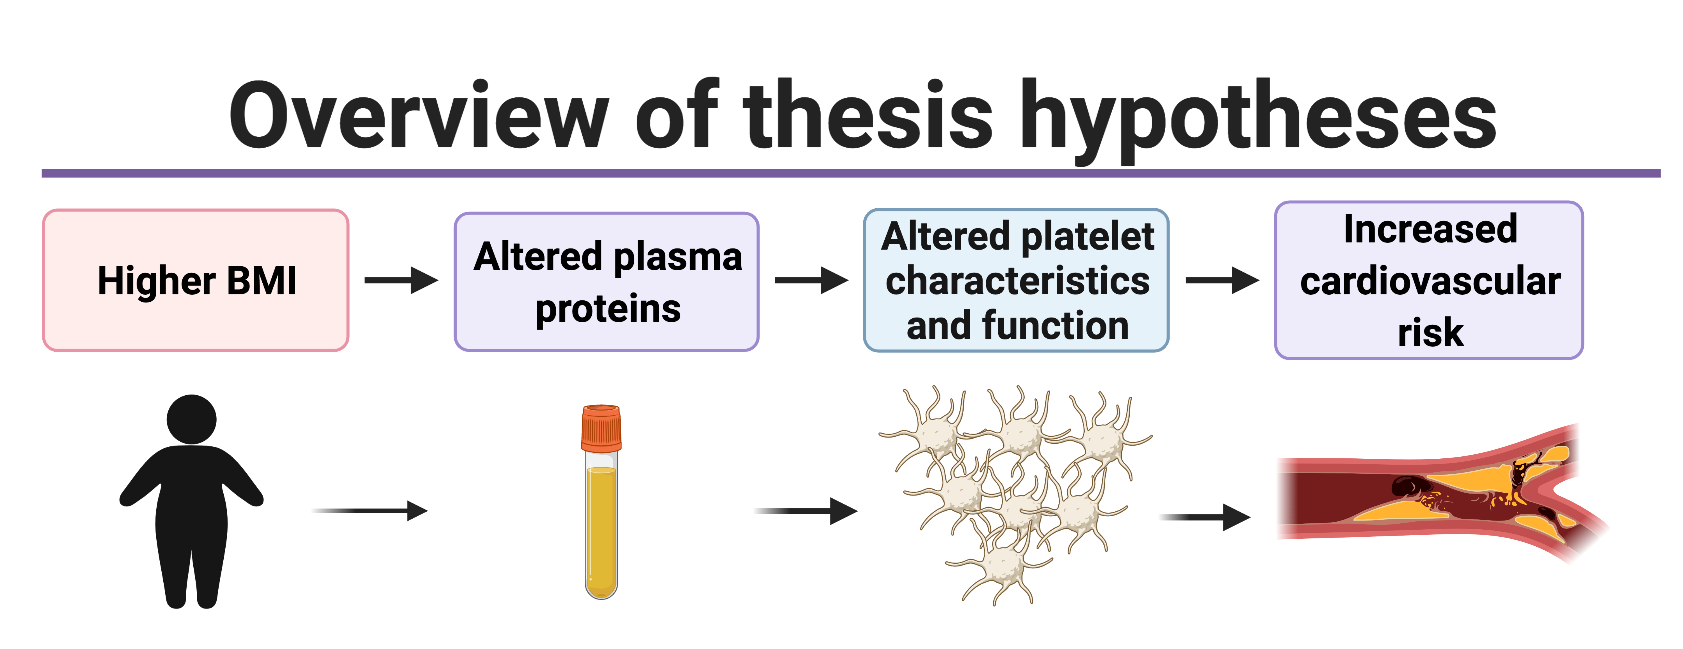
\includegraphics{figure/Intro_background/Thesis_graphic_overview_without_chapters} 

}

\caption[Schematic of the multi-step pathway addressed in the thesis]{\textbf{Schematic of the multi-step pathway addressed in the thesis}}\label{fig:Thesis-schematic}
\end{figure}
\hypertarget{thesis-structure}{%
\section{Thesis structure}\label{thesis-structure}}

To address the thesis aims, there will be six results chapters in this thesis:
\begin{enumerate}
\def\labelenumi{\arabic{enumi})}
\tightlist
\item
  Using observational and MR frameworks to determine the effect of body mass index on platelet characteristics (Chapter \ref{BMI-platelets-INTERVAL})
\item
  The effect of obesity on platelet function: a clinical pilot study (Chapter \ref{BMI-platelets-clinic})
\item
  Pathways linking plasma proteins and platelet function: do the chemokines MDC and TARC play a role? (Chapter \ref{chemokine-platelets})
\item
  Exploring the plasma proteome as a link between adiposity and platelet function: Observational and Mendelian randomization estimates (Chapter \ref{BMI-protein-MR})
\item
  Further elucidating the effect of adiposity on the plasma proteome using a weight loss intervention (Chapter \ref{BMI-protein-RCT})
\item
  Combining MR and an RCT to determine effects of adiposity on the plasma proteome. (Chapter \ref{Comparison-proteome})
\end{enumerate}
\hypertarget{BMI-platelets-INTERVAL}{%
\chapter{Using observational and MR frameworks to determine the effect of body mass index on platelet characteristics}\label{BMI-platelets-INTERVAL}}

This work is published in the journal Platelets\textsuperscript{\protect\hyperlink{ref-Goudswaard2022}{96}}. I performed all analyses, created all figures and tables and wrote the manuscript.

\hypertarget{background-1}{%
\section{Background}\label{background-1}}

The introduction chapter (Chapter \ref{background}) indicated that clinical studies and genetic association studies have identified BMI as an independent risk factor for thrombotic disorders such as CHD and stroke\textsuperscript{\protect\hyperlink{ref-Nordestgaard2012}{11},\protect\hyperlink{ref-Dale2017}{28},\protect\hyperlink{ref-Wolk2003a}{97}}. Platelet hyperactivity can be an indicator of those who may be at an increased risk of thrombosis\textsuperscript{\protect\hyperlink{ref-Puurunen2018}{98}}. There is evidence that people with a higher BMI have hyperactive platelets\textsuperscript{\protect\hyperlink{ref-Nardin2015}{44},\protect\hyperlink{ref-Barrachina2019}{99}}, which could explain why a higher BMI is linked to an increase in thrombosis. Platelet function can be directly assessed by various methods (section \ref{platelet-function-techniques}, but these techniques are not widely available or readily standardized. Haematology analyzers such as the Sysmex XN series are more commonly used to provide full blood counts, providing detailed readouts of platelet characteristics. Mechanisms of platelet hyperactivity are unclear, but it is possible that alterations in properties of platelets such as PLT, MPV and IPF/IPC may contribute to the phenotype.

Immature platelets (also known as reticulated platelets) are the youngest platelets in circulation and are detected based on having a greater forward scatter (FSC, an indicator of their size) and a greater side fluorescence (SFL, an indicator of their mRNA content)\textsuperscript{\protect\hyperlink{ref-Ibrahim2014}{72}}. More immature platelets are indicative of enhanced platelet production\textsuperscript{\protect\hyperlink{ref-Lev2016a}{100}} and these platelets are believed to be more prothrombotic than older circulating platelets, with more dense granule release and increased P-selectin expression\textsuperscript{\protect\hyperlink{ref-Ibrahim2014}{72},\protect\hyperlink{ref-Lev2016a}{100},\protect\hyperlink{ref-Bernlochner2015a}{101}}. Higher immature platelet count is associated with adverse cardiovascular outcomes in patients with coronary artery disease\textsuperscript{\protect\hyperlink{ref-Ibrahim2014}{72}} and reduced effectiveness of antiplatelet therapies\textsuperscript{\protect\hyperlink{ref-Bernlochner2015a}{101},\protect\hyperlink{ref-Ibrahim2012}{102}}, suggesting that hyperactive immature platelets may contribute to adverse vascular events. Immature platelets have also been suggested to be less responsive to antiplatelet therapies such as prasugrel in acute coronary syndrome patients\textsuperscript{\protect\hyperlink{ref-Bernlochner2015a}{101}}.

As these platelet characteristics provide potential information about platelet hyperactivity and given the increased thrombotic risk seen with adiposity, it is important to assess how adiposity affects platelet properties. Previous studies with modest samples sizes have implemented observational epidemiological methods to explore the effect of BMI on PLT, plateletcrit (PCT) and MPV. There is conflicting observational evidence regarding an association between BMI and PLT\textsuperscript{\protect\hyperlink{ref-Furuncuoglu2016}{67},\protect\hyperlink{ref-Han2018a}{68}}, with some studies suggesting a positive association between BMI and MPV\textsuperscript{\protect\hyperlink{ref-Coban2005}{69}} and other studies reporting no such association\textsuperscript{\protect\hyperlink{ref-Heffron2018}{70}}. Furthermore, as there is evidence that immature platelet production is increased in patients with metabolic syndrome and type II diabetes\textsuperscript{\protect\hyperlink{ref-Vaduganathan2008a}{103},\protect\hyperlink{ref-Mijovic2015a}{104}}, it is therefore important to explore whether BMI may be an independent predictor of this trait. It is currently unknown whether the influence of BMI on platelet properties and function are causal and independent of confounding effects.

In this chapter, data from the INTERVAL prospective cohort (N=33388) was used to explore the association between BMI and platelet traits. Figure \ref{fig:BMI-platelet-overview} shows the associations of the overall thesis hypothesis addressed in the chapter. Here, observational and Mendelian randomization (MR) approaches were employed to test the hypothesis that higher BMI leads to changes in platelet characteristics. Although observational studies can demonstrate associations between BMI and platelet characteristics, they cannot determine direct causality. To address the latter, we therefore employed MR, using a genetic risk score derived from single nucleotide polymorphisms (SNPs) associated with higher BMI (Figure \ref{fig:Linear-reg-MR}). This allowed estimation of the causal effect of BMI on platelet traits, reducing the effect of confounding factors that are inherent to observational studies. To assess functional implications of BMI-platelet associations, a follow-up analysis was designed to explore the associations between platelet characteristics and whole blood aggregation in a cohort of cardiac surgery patients.



\begin{figure}

{\centering \includegraphics[width=0.8\linewidth]{figure/BMI_platelets/Thesis_graphic_overview_BMI_platelets} 

}

\caption[Schematic of the associations explored in the current chapter: the relationship between body mass index and platelet traits.]{\textbf{Schematic of the associations explored in the current chapter: the relationship between body mass index and platelet traits.} Figure made using BioRender.com.}\label{fig:BMI-platelet-overview}
\end{figure}


\begin{figure}

{\centering \includegraphics[width=0.8\linewidth]{figure/BMI_platelets/obsvMRexample} 

}

\caption[Schematic of linear regression and Mendelian randomization frameworks for BMI and platelet trait analyses]{\textbf{Schematic of linear regression and Mendelian randomization analyses. Linear regression assesses the association between BMI (exposure) and platelet traits (outcome), with adjustment for potential confounders.} Under the assumptions of Mendelian randomization (MR), the genetic risk score (GRS) for body mass index (BMI) does not associate with confounding variables, and if there is a causal association, the GRS should only associate with platelet outcomes through its association with body mass index.}\label{fig:Linear-reg-MR}
\end{figure}
\hypertarget{methods}{%
\section{Methods}\label{methods}}

\hypertarget{INTERVAL-study}{%
\section{The INTERVAL study}\label{INTERVAL-study}}

\hypertarget{study-overview}{%
\subsection{Study overview}\label{study-overview}}

INTERVAL is a prospective cohort study that initially aimed to test the safety of reducing the time interval between donation of whole blood in 50,000 participants\textsuperscript{\protect\hyperlink{ref-DiAngelantonio2017}{105}}. Participants were over the age of 18 years, able to provide informed consent and free from a history of major disease. Participants were recruited between June 11th, 2012 and June 15th, 2014 from 25 National Health Service Blood and Transplant (NHSBT) centres across England. They filled out online questionnaires including self-reported height and weight, smoking status and alcohol consumption. Blood samples were also taken at baseline (before randomization within the study) where full blood counts were obtained. The study was approved by Cambridge East Research Ethics Committee. Permission for data access was provided by the Data Access Committee. Data contains sensitive content and requires permission to use therefore cannot be made publicly available. Access to data needs to be approved by the INTERVAL team www.intervalstudy.org.uk/more-information.

\hypertarget{assessment-of-bmi-and-covariables}{%
\subsection{Assessment of BMI and covariables}\label{assessment-of-bmi-and-covariables}}

Participants completed online questionnaires wherein they reported their height and weight. BMI was calculated as weight in kilograms divided by the square of their height in metres (kg/m\textsuperscript{2}). Available covariables were age, sex, previous or current smoking frequency (in three categories of: never, occasional, most days or every day) and alcohol intake frequency (in four categories of: rarely, less than once a week, 1-2 times a week, 3-5 times a week or most days for the proteomics analysis, or three categories of never, previous and current in the platelet trait analysis). These covariables were chosen as they were measured in the INTERVAL collection and are measures which are thought to influence adiposity and cardiometabolic health\textsuperscript{\protect\hyperlink{ref-Bell2018a}{31}}.

\hypertarget{genetic-data-and-instrument-for-bmi}{%
\subsection{Genetic data and instrument for BMI}\label{genetic-data-and-instrument-for-bmi}}

INTERVAL participant genotyping was performed on the Affymetrix GeneTitan Multi-Channel (MC) Instrument using the UK Biobank Axiom Array (ThermoFisher Scientific, Loughborough, UK) and the QC of genotype data was implemented as described by Astle et al.~=.\textsuperscript{\protect\hyperlink{ref-Astle2016}{106}} The imputation panel used was the 1000 genomes phase-3-UK-10K\textsuperscript{\protect\hyperlink{ref-Astle2016}{106}}. A genetic instrument for BMI was constructed using 654 genetic variants that were associated with BMI at P\textless5x10\textsuperscript{-8} in the inverse variance weighted fixed-effect meta-analysis of GWAS of 700000 individuals of European ancestry\textsuperscript{\protect\hyperlink{ref-Yengo2018}{21}}. This meta-analysis consisted of around 250000 adults from the Genetic Investigation of ANthromopetric Traits (GIANT) consortium\textsuperscript{\protect\hyperlink{ref-Locke2015}{20}} and 450000 adults from the UK Biobank study. Only 0.05 \% of UK Biobank participants were included in the current INTERVAL study (of N=2737). These participants were not excluded to increase power. The weighted GRS was made using PLINK 2.0 software\textsuperscript{\protect\hyperlink{ref-Purcell2007a}{107}} using the effect alleles and beta coefficients from the source GWAS. The score was calculated by multiplying the number of effect alleles at each SNP by its effect estimate (beta), summing these, and dividing by the total number of SNPs included. The GRS therefore can be interpreted as the average per-SNP effect on BMI for each individual.

\hypertarget{study-population}{%
\subsection{Study population}\label{study-population}}

The present study was conducted on up to 33388 European ancestry INTERVAL participants living in the United Kingdom. These were the participants who had genetic data, had basic phenotype data and full blood count measures (Figure \ref{fig:INTERVAL-STROBE}).




\begin{figure}

{\centering 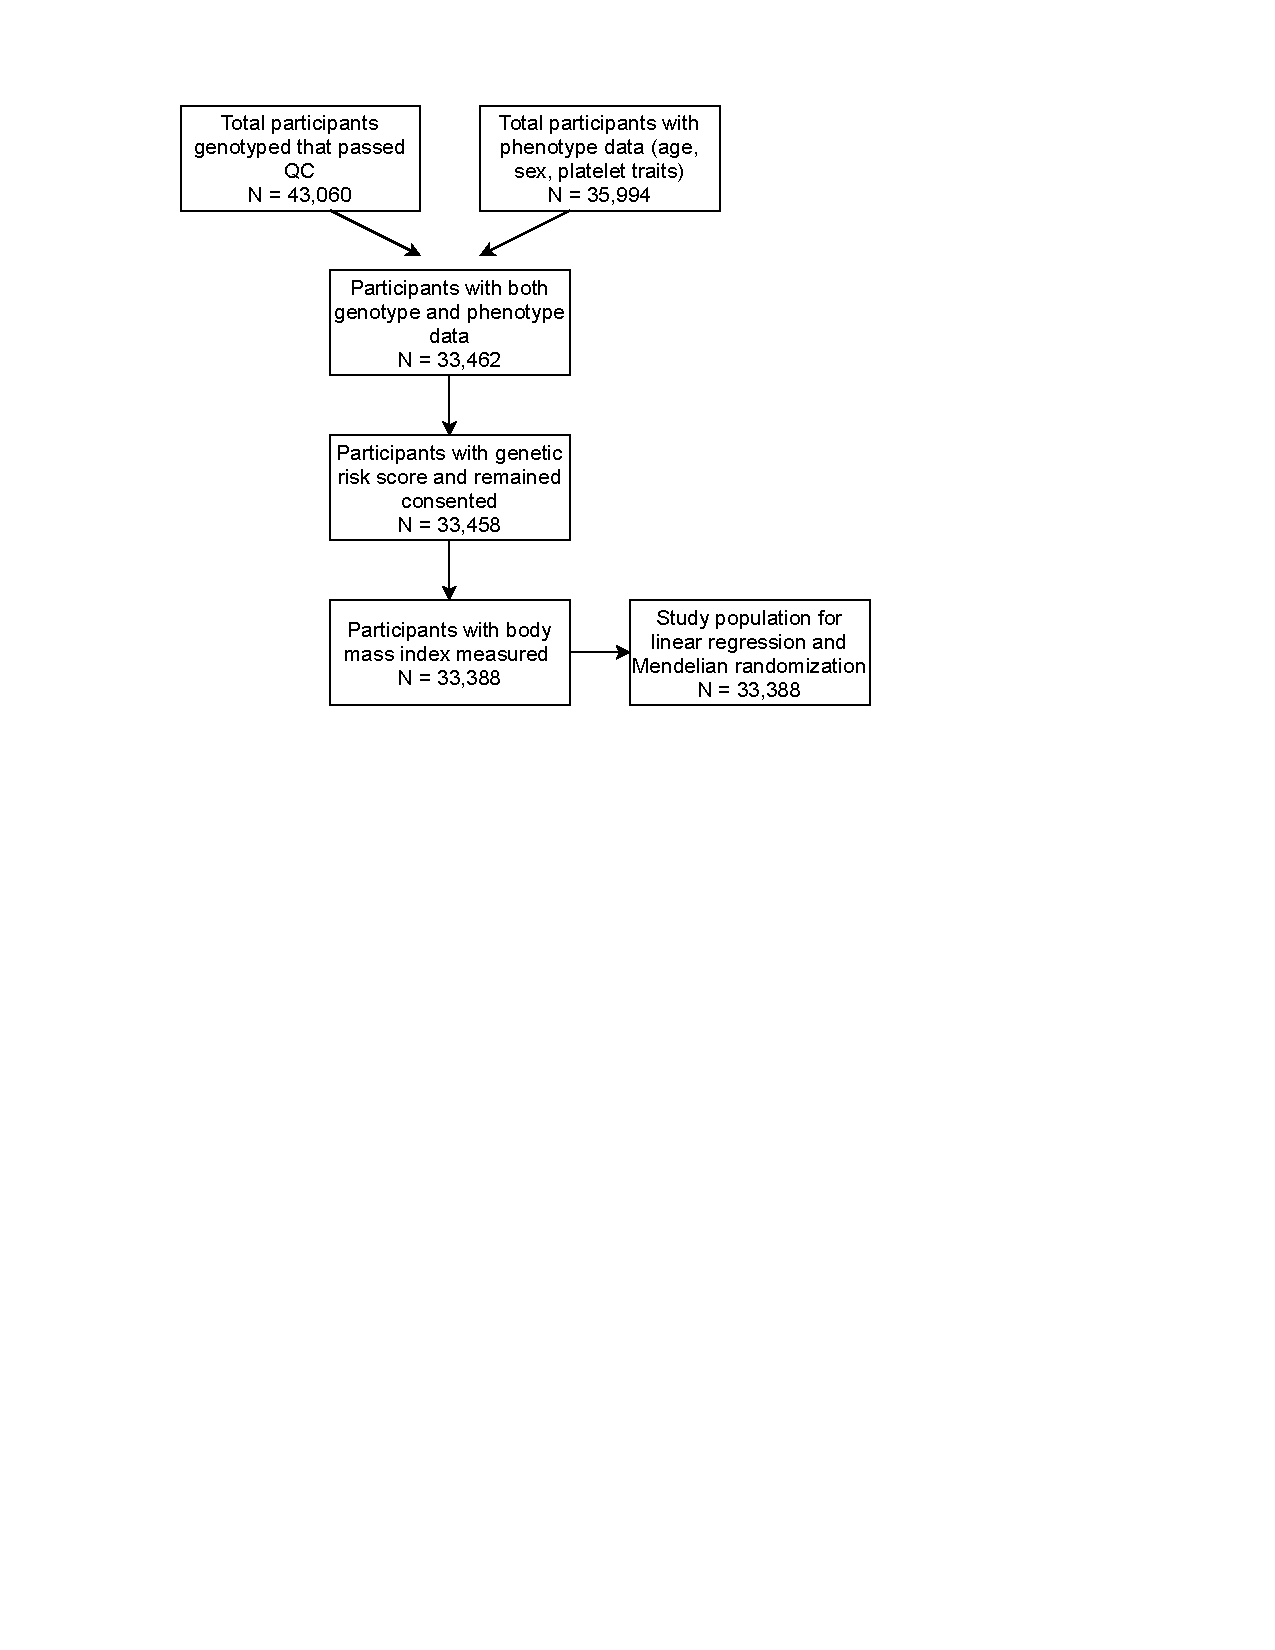
\includegraphics[width=0.6\linewidth]{figure/BMI_platelets/STROBE_diagram} 

}

\caption[A STROBE diagram outlining participants included in the INTERVAL study for BMI and platelet trait analyses.]{\textbf{A STROBE diagram outlining participants included in the INTERVAL study for BMI and platelet trait analyses}.}\label{fig:INTERVAL-STROBE}
\end{figure}
\hypertarget{measurement-of-platelet-traits}{%
\subsection{Measurement of platelet traits}\label{measurement-of-platelet-traits}}

Blood was taken by venipuncture into 3mL ethylenediamine tetraacetic acid (EDTA) tubes. Platelet parameters were measured using the Sysmex XN-1000 instrument\textsuperscript{\protect\hyperlink{ref-Astle2016}{106}}. This analyzer provides information on cell counts by using a combination of fluorescence (PLT-F) and impedance (I) flow cytometry. The PLT-F channel used a Fluorocell fluorescent dye (oxazine), whereas the impedance method uses electrical resistance to detect platelets. Platelet indices included in the current study, along with the raw units, are provided in Table \ref{tab:Platelet-traits}. These measurements were pre-adjusted for technical covariates such as time between venipuncture and blood count, as well as instrument drift, seasonal and weekly variation\textsuperscript{\protect\hyperlink{ref-Astle2016}{106}}. Adjustment was performed with cyclic, thin-plate and P-splines in a generalized additive model (GAM)\textsuperscript{\protect\hyperlink{ref-Akbari2020}{108}}. Resulting platelet trait values along with their units of measurement are reported in Table \ref{tab:Platelet-traits}. These data were rank normal transformed to normalize the distribution of each trait. Therefore, each platelet index is measured in normalized standard deviation (SD) units.




\begin{landscape}\begin{table}

\caption[Platelet traits measured by Sysmex XN-1000]{\label{tab:Platelet-traits}\textbf{Platelet traits measured by Sysmex XN-1000}.}
\centering
\begin{tabu} to \linewidth {>{\raggedright}X>{\raggedright\arraybackslash}p{4cm}>{\raggedright\arraybackslash}p{6cm}>{\raggedright}X>{\raggedright}X}
\toprule
Short name & Full name & Derivation of platelet trait & Units & Mean (SD)\\
\midrule
P-LCR & Platelet large cell ratio & (platelet number with volume>12 fL)/(platelet number of ordinary volume)  x 100 & \% & 36.9 (7.7)\\
H-IPF & High fluorescence immature platelet fraction & (high fluorescence immature platelet number)/(platelet count)  x 100 & \% & 1.3 (1.0)\\
PLT (F) & Platelet count (PLT-F channel) & Total number of platelets per litre & 10E9/L & 255 (57)\\
PLT (I) & Platelet count (impedance channel) & Total number of platelets per litre & 10E9/L & 250 (55)\\
PCT & Plateletcrit & Volume percentage of blood occupied by platelets & \% & 0.28 (0.06)\\
\addlinespace
PDW & Platelet distribution width & Standard deviation of platelet volume distribution, estimated as width at 20\% modal height of platelet volume histogram & fL & 14.0 (1.8)\\
IPC & Immature platelet count & Immature platelet count & 10E9/L & 10.1 (5.0)\\
IPF & Immature platelet fraction & (Immature platelet number)/(platelet count)   x 100 & \% & 4.2 (2.5)\\
MPV & Mean platelet volume & Mean platelet volume & fL & 11.1 (1.0)\\
SFL & Side fluorescence & Side fluorescence measures the nucleic acid (mRNA) content of the platelet & RFUs & 80.3 (5.0)\\
\addlinespace
FSC & Forward scatter & Forward scatter is a measure of the size of the platelet & RFUs & 53.0 (6.4)\\
SSC & Side scatter & Side scatter is a measure of the granularity of the platelet & RFUs & 37.9 (2.9)\\
\bottomrule
\end{tabu}
\end{table}
\end{landscape}
\hypertarget{statistical-analysis}{%
\subsection{Statistical analysis}\label{statistical-analysis}}

Analyses were performed using R version 3.4.2\textsuperscript{\protect\hyperlink{ref-Team2019a}{109}}. To visualize correlation between outcome platelet variables, a correlation matrix was made using the pairwise Pearson correlation coefficients of the rank normal transformed data. A dendrogram was also created to show the hierarchical relationship between platelet traits (\url{https://github.com/hughesevoanth/iPVs}), where the height at which variables are joined is set at (1 -- Pearson correlation coefficient (r)). To explore observational associations between BMI and platelet traits, linear regression models were used (lm() function from ``stats'' package). Two regression models were used: firstly, adjusting for age and sex and secondly, additionally adjusting for smoking and alcohol consumption as ordinal variables. The results of the regression reflect the change in platelet traits (in normalized SD units) per normalized SD higher BMI (4.7 kg/m\textsuperscript{2}). Only participants with all covariables were included in the linear regression models. The associations between potential covariables with both BMI and platelet traits were also explored using linear regression.

To understand properties of the GRS for BMI, the association between the GRS with both BMI and covariables were explored. The MR analysis was performed by using a two-stage least squares (2SLS) regression model (using systemfit() function from ``systemfit'' package\textsuperscript{\protect\hyperlink{ref-Henningsen2007}{110}}). The MR causal estimates reflect the change in platelet traits (in SD units) per SD increase in BMI. A Wu-Hausman test was performed to test for endogeneity between observational and MR estimates. Exact beta coefficients, confidence intervals and P values are provided throughout and guide strength of association.

Where there was consistent observational and MR evidence for a BMI effect on platelet traits with potential clinical relevance, additional sensitivity analyses were carried out. We explored whether there were different magnitudes of associations across NHS BMI categories indicative of a non-linear relationship. Specifically, participants were stratified by BMI and the association between BMI and IPC estimated within BMI categories.

\hypertarget{follow-up-analysis-to-explore-the-association-between-immature-platelets-and-aggregation}{%
\subsection{Follow-up analysis to explore the association between immature platelets and aggregation}\label{follow-up-analysis-to-explore-the-association-between-immature-platelets-and-aggregation}}

Motivated by findings from the primary analyses described above, additional observational analyses were conducted using data from the COagulation and Platelet laboratory Testing in Cardiac Surgery (COPTIC) study. The COPTIC study was an observational, single centre cohort study of adults undergoing cardiac surgery at the Bristol Heart Institute with primary objective of examining the relationship between coagulation laboratory parameters and bleeding outcomes after surgery in 2,541 participants\textsuperscript{\protect\hyperlink{ref-Mumford2017}{111}}. This study was approved by the UK NHS Research Ethics Committee (09/H0104/53).

\hypertarget{coptic-study-variables}{%
\subsection{COPTIC study variables}\label{coptic-study-variables}}

Age and sex were reported at baseline. Height and weight were obtained from medical notes. BMI was derived from weight and height (kg/m\textsuperscript{2}). Smoking was reported as a categorical variable (0=never smoker, 1=ex-smoker for \textgreater{} 5 years, 2=ex-smoker for 1-5 years, 3=ex-smoker for 30 days-1 year, 4=current smoker). Platelet variables (PLT, MPV, IPF, IPC) were measured using the Sysmex XE-2100 Automated Haematology System (Oxford, UK). Blood samples were taken pre-operatively into 3.2\% sodium citrate vacutainers (BD Biosciences, Milton Keynes, UK). Platelet aggregation was measured using Multiplate multiple electrode aggregometry (MEA) (Roche, Rotkreuz, Switzerland), which detects change in electrical impedance when platelets aggregate on metal electrodes. Aggregation was determined by the area under the curve (AUC) in response to platelet agonists including adrenaline (100 mg/mL), thrombin receptor activator peptide 6 test (TRAP-test), ADP-test and arachidonic acid (ASPI-test). Use of a combination of agonists therefore reflects activation of platelets via different pathways: adrenaline acts at the α2 adrenergic receptor, TRAP-6 acts at the protease-activated receptor-1 (PAR-1), ADP acts at the P2Y12 receptor and arachidonic acid at the Thromboxane A2 (TxA2) receptor.

\hypertarget{coptic-statistical-analysis}{%
\subsection{COPTIC statistical analysis}\label{coptic-statistical-analysis}}

The COPTIC dataset in the current analysis included 2,518 participants (23 out of 2,541 participants did not consent for future research). For the current study, only those who were not on antiplatelet therapies (prasugrel, clopidogrel or aspirin) were included (N=655). Extreme outliers that were ± 5 SDs from the mean were removed, and exposures and outcomes were rank normal transformed. Linear regression was used to generate estimates of the association between BMI and platelet parameters within this cohort. Linear regression was used to explore the association between immature platelet count and aggregation, adjusting for age, sex and smoking status.

\hypertarget{results}{%
\section{Results}\label{results}}

\hypertarget{interval-participant-characteristics}{%
\subsection{INTERVAL participant characteristics}\label{interval-participant-characteristics}}

Of INTERVAL participants included in the current study (N=33,388), 50.2 \% were female. The mean age was 45.3 years (SD of 14.2 years, Table \ref{tab:INT-participants-platelets}). The mean BMI was 26.4 kg/m\textsuperscript{2} (SD of 4.7 kg/m\textsuperscript{2}). The majority of participants were never smokers (58.9 \%), with 33.3\% and 7.8 \% reported as previous and current smokers, respectively. Nearly a third (32.7 \%) of participants reported drinking alcohol at least three times a week.




\begin{table}

\caption[Characteristics of included INTERVAL participants for BMI-platelet analyses]{\label{tab:INT-participants-platelets}\textbf{Characteristics of included INTERVAL participants for BMI-platelet analyses}}
\centering
\begin{tabu} to \linewidth {>{\raggedright\arraybackslash}p{8cm}>{\raggedright}X>{\raggedleft}X}
\toprule
Variable & Mean (SD) or \% & N\\
\midrule
Age & 45.3 (14.2) & 33388\\
Sex &  & 33388\\
\hspace{1em}Male & 49.8\% & \\
\hspace{1em}Female & 50.2\% & \\
Weight (kg) & 78.2 (16.0) & 33455\\
\addlinespace
Height (cm) & 171.8 (9.6) & 33388\\
Body mass index (kg/m2) & 26.4 (4.7) & 33388\\
Smoking frequency &  & 32867\\
\hspace{1em}Never & 58.9\% & \\
\hspace{1em}Previous & 33.3\% & \\
\addlinespace
\hspace{1em}Current & 7.8\% & \\
Alcohol intake frequency &  & 29538\\
\hspace{1em}Rarely & 12.5\% & \\
\hspace{1em}Less than once a week & 17.1\% & \\
\hspace{1em}One or two times a week & 37.7\% & \\
\addlinespace
\hspace{1em}Three to five times a week / most days & 32.7\% & \\
\bottomrule
\end{tabu}
\end{table}
\hypertarget{correlation-between-platelet-traits-in-interval}{%
\subsection{Correlation between platelet traits in INTERVAL}\label{correlation-between-platelet-traits-in-interval}}

The Sysmex XN-1000 haematology analyzer measures multiple platelet traits, however many of these traits are closely related measurements and therefore may not be completely independent. Indeed, platelet traits showed a high degree of correlation with each other (Figure \ref{fig:Corr-mat-dend}), in particular among similar measures. For example, measures of PLT (PLT I/F) and PCT, the latter a measurement of platelet mass, were highly positively correlated with each other but were weakly inversely correlated with other platelet measures. Measures of platelet maturity (IPF, IPC, H-IPF) were highly correlated with each other. In addition, platelet size variables (MPV, P-LCR and PDW) showed strong positive correlations with each other as well as with measures of immature platelets.




\begin{figure}

{\centering 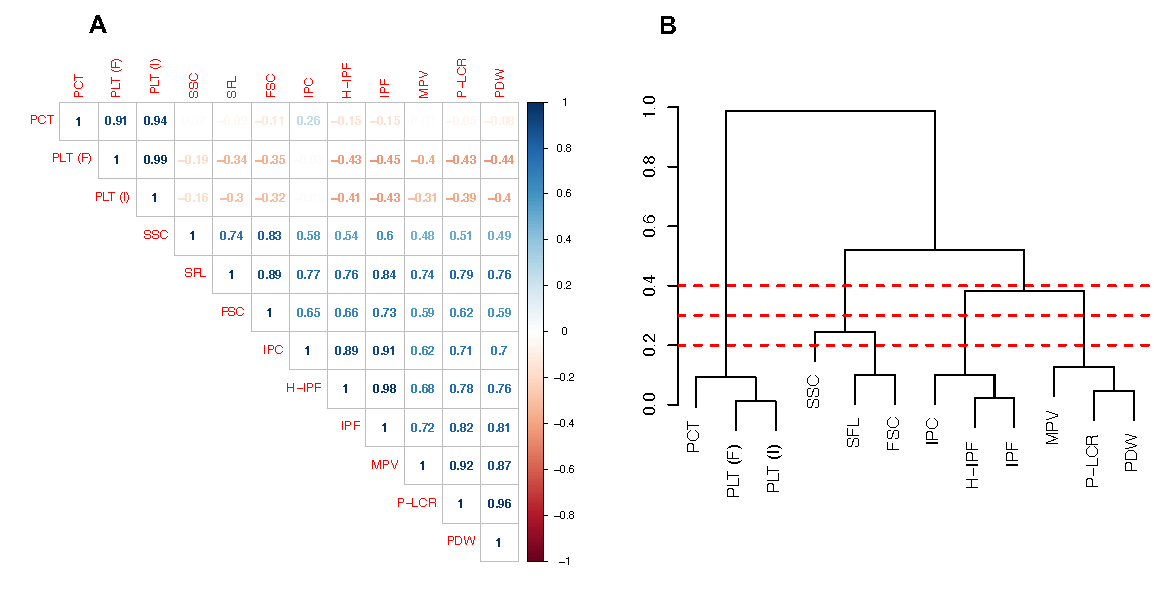
\includegraphics[width=0.95\linewidth]{figure/BMI_platelets/Corrmatrix_dendrogram} 

}

\caption[Correlation matrix and dendrogram of the relationship between platelet traits]{\textbf{Correlation matrix and dendrogram of the relationship between platelet traits.} A) Correlation coefficients are provided within the matrix. Dark blue indicates a correlation coefficient (r) of 1, with dark red indicating a correlation coefficient of -1. B) A dendrogram showing the hierarchical relationship between platelet traits, where the height at which two platelet traits join is (1 -- Pearson correlation coefficient (r)). PCT = plateletcrit, PLT (F) = platelet count (PLT-F channel), PLT (I) = platelet count (impedance channel), SSC = side scatter, SFL = side fluorescence, FSC = side scatter, IPC = immature platelet count, H-IPF = high fluorescence immature platelet fraction, IPF = immature platelet fraction, MPV = mean platelet volume, P-LCR = platelet large cell ratio, PDW = platelet distribution width. Dashed red lines indicate a height of 0.2, 0.3 and 0.4.}\label{fig:Corr-mat-dend}
\end{figure}
\hypertarget{observational-associations-between-bmi-and-platelet-traits-in-interval}{%
\subsection{Observational associations between BMI and platelet traits in INTERVAL}\label{observational-associations-between-bmi-and-platelet-traits-in-interval}}

Linear regression was performed to determine whether a higher BMI was associated with a change in platelet characteristics. In the confounder adjusted linear regression (Table \ref{tab:BMI-platelets-adjust}), BMI was positively associated with PCT (0.12 SD higher per SD higher BMI, 95\% CI 0.11 to 0.13, P = 9.2 x 10\textsuperscript{-88}) and platelet count (PLT (I) 0.11 SD higher per SD higher BMI, 95\% CI 0.09 to 0.12, P = 1.0 x 10\textsuperscript{-67}). The next strongest association with BMI was the association with SFL (0.06 SD higher per SD increase in BMI, 95\% CI 0.05 to 0.07, P = 4.7x10\textsuperscript{-23}). BMI also showed a positive association with IPC (0.06 SD higher per SD increase in BMI, 95\% CI 0.05 to 0.08, P = 4.8x10\textsuperscript{-22}). These results demonstrate that BMI is positively associated with PCT, PLT (I), SFL and IPC in this population. These estimates were very similar to the age and sex only adjusted estimates (Table \ref{tab:BMI-platelets-unadjust}).




\begin{landscape}\begin{table}

\caption[Observational associations between BMI and platelet measures adjusted for age, sex, smoking status and alcohol consumption]{\label{tab:BMI-platelets-adjust}\textbf{Observational associations between BMI and platelet measures adjusted for age, sex, smoking status and alcohol consumption.} Βeta coefficient is the change in platelet measure in SDs per normalized SD increase in BMI. PCT = plateletcrit, PLT (I) = platelet count (impedance channel), PLT (F) = platelet count (PLT-F channel), SFL = side fluorescence, IPC = immature platelet count, PDW = platelet distribution width, FSC = forward scatter, H-IPF = high fluorescence immature platelet fraction, IPF = immature platelet fraction, P-LCR = platelet large cell ration, SSC = side scatter, MPV = mean platelet volume. Eta squared is the proportion of variance explained by the platelet trait in an ANOVA, whereas adjusted R squared is the variance explained by all the predictor variables in the regression model.}
\centering
\begin{tabu} to \linewidth {>{\raggedright}X>{\raggedright}X>{\raggedright}X>{\raggedright}X>{\raggedright}X>{\raggedright}X>{\raggedright}X>{\raggedright}X>{\raggedright}X>{\raggedright}X}
\toprule
Platelet trait & N & Βeta coefficient & SE & P value & R2 & Eta2 & 95\% CI & Lower 95\% CI & Upper 95\% CI\\
\midrule
PCT & 24562 & 0.12 & 0.006 & 9.17e-88 & 0.133 & 0.107 & 0.012 & 0.11 & 0.13\\
PLT (I) & 26044 & 0.11 & 0.006 & 1.03e-67 & 0.096 & 0.081 & 0.012 & 0.09 & 0.12\\
PLT (F) & 23921 & 0.1 & 0.006 & 5.62e-57 & 0.094 & 0.082 & 0.012 & 0.09 & 0.11\\
SFL & 26082 & 0.06 & 0.006 & 4.73e-23 & 0.02 & 0.000 & 0.012 & 0.05 & 0.07\\
IPC & 23909 & 0.06 & 0.007 & 4.84e-22 & 0.008 & 0.001 & 0.013 & 0.05 & 0.08\\
\addlinespace
PDW & 24563 & 0.03 & 0.007 & 5.21e-05 & 0.006 & 0.004 & 0.013 & 0.01 & 0.04\\
FSC & 26082 & 0.02 & 0.006 & 0.01 & 0.026 & 0.001 & 0.012 & 0.01 & 0.03\\
H-IPF & 26068 & -0.02 & 0.006 & 0.01 & 0.006 & 0.005 & 0.012 & -0.03 & -0.01\\
IPF & 23909 & 0.01 & 0.007 & 0.04 & 0.008 & 0.007 & 0.013 & 0.00 & 0.03\\
P-LCR & 27015 & 0.01 & 0.006 & 0.19 & 0.003 & 0.000 & 0.012 & 0.00 & 0.02\\
\addlinespace
SSC & 26082 & 0.01 & 0.006 & 0.28 & 0.04 & 0.000 & 0.012 & -0.01 & 0.02\\
MPV & 24559 & 0.01 & 0.007 & 0.37 & 0.007 & 0.000 & 0.013 & -0.01 & 0.02\\
\bottomrule
\end{tabu}
\end{table}
\end{landscape}



\begin{landscape}\begin{table}

\caption[Age and sex adjusted estimates for the association between BMI and platelet traits]{\label{tab:BMI-platelets-unadjust}\textbf{Age and sex adjusted estimates for the association between BMI and platelet traits.} Βeta coefficient is the change in platelet measure in SDs per SD higher BMI. Eta squared is the proportion of variance explained by the platelet trait in an ANOVA, whereas adjusted R squared is the variance explained by all the predictor variables in the regression model.}
\centering
\begin{tabu} to \linewidth {>{\raggedright\arraybackslash}p{3.5cm}>{\raggedright}X>{\raggedright}X>{\raggedright}X>{\raggedright}X>{\raggedright}X>{\raggedright}X>{\raggedright}X>{\raggedright}X>{\raggedright}X>{\raggedright}X}
\toprule
Full name & Short Name & N & Beta coefficient & SE & P value & R2 & Eta2 & 95\% CI & Lower 95\% CI & Upper 95\% CI\\
\midrule
Plateletcrit & PCT & 27997 & 0.126 & 0.006 & 1.46e-108 & 0.132 & 0.107 & 0.011 & 0.115 & 0.137\\
Platelet count (impedence channel) & PLT (I) & 29682 & 0.11 & 0.006 & 4.5e-84 & 0.097 & 0.082 & 0.011 & 0.099 & 0.121\\
Platelet count (PLT-F channel) & PLT (F) & 27268 & 0.104 & 0.006 & 6.5e-70 & 0.094 & 0.083 & 0.012 & 0.093 & 0.116\\
Side fluorescence & SFL & 29721 & 0.064 & 0.006 & 4.08e-28 & 0.021 & 0.000 & 0.011 & 0.053 & 0.076\\
Immature platelet count & IPC & 27255 & 0.067 & 0.006 & 1.27e-27 & 0.007 & 0.001 & 0.012 & 0.055 & 0.079\\
\addlinespace
Platelet distribution width & PDW & 27998 & 0.029 & 0.006 & 2.09e-06 & 0.006 & 0.004 & 0.012 & 0.017 & 0.041\\
Forward scatter & FSC & 29721 & 0.022 & 0.006 & 0.00014 & 0.026 & 0.001 & 0.011 & 0.011 & 0.034\\
High fluorescence immature platelet fraction & H-IPF & 29708 & -0.017 & 0.006 & 0.00443 & 0.005 & 0.005 & 0.012 & -0.028 & -0.005\\
Immature platelet fraction & IPF & 27255 & 0.015 & 0.006 & 0.0129 & 0.007 & 0.007 & 0.012 & 0.003 & 0.027\\
Side scatter & P-LCR & 29721 & 0.01 & 0.006 & 0.0781 & 0.041 & 0.000158 & 0.011 & -0.001 & 0.022\\
\addlinespace
Platelet large cell ratio & SSC & 30788 & 0.01 & 0.006 & 0.0909 & 0.002 & 4.37e-05 & 0.011 & -0.002 & 0.021\\
Mean platelet volume & MPV & 27994 & 0.009 & 0.006 & 0.155 & 0.006 & 4.57e-06 & 0.012 & -0.003 & 0.021\\
\bottomrule
\end{tabu}
\end{table}
\end{landscape}
\hypertarget{associations-of-covariables-with-bmi-and-platelet-traits-in-interval}{%
\subsection{Associations of covariables with BMI and platelet traits in INTERVAL}\label{associations-of-covariables-with-bmi-and-platelet-traits-in-interval}}

The association of covariables (age, sex, smoking and alcohol) with BMI were evaluated (Table \ref{tab:INT-confounders-BMI-platelets}). Included covariables in the analysis showed associations with BMI. Males had a higher BMI than females (0.18 SD, 95\% CI 0.16 to 0.21, P = 9.64x10\textsuperscript{-64}). Age was positively associated with BMI (0.011 SD higher per year older, 95\% CI 0.010 to 0.012, P = 1.11x10\textsuperscript{-182}). Alcohol showed an inverse association with BMI and smoking showed a weak positive association with BMI. Associations between covariables (age, sex, smoking, alcohol) and platelet traits were also explored (Figure \ref{fig:confounder-platelets}). Higher age was generally inversely associated with platelet measures. Males had a lower platelet count and PCT compared to females (PLT-F was 0.57 lower 95\% CI -0.60 to -0.55, P = 9.9x10\textsuperscript{-324}). Weak associations were detected between smoking and platelet traits such as a positive association between smoking status and immature platelets. Higher alcohol consumption also showed inverse associations with measures of PCT and PLT.




\begin{table}

\caption[Associations between age, sex, smoking and alcohol consumption (exposures) with standardised BMI (outcome).]{\label{tab:INT-confounders-BMI-platelets}\textbf{Associations between age, sex, smoking and alcohol consumption (exposures) with standardised BMI (outcome).} Beta coefficient is the change in BMI (normalized SDs) per unit increase in exposure.}
\centering
\fontsize{8}{10}\selectfont
\begin{tabu} to \linewidth {>{\raggedright\arraybackslash}p{4cm}>{\raggedright}X>{\raggedright\arraybackslash}p{2cm}>{\raggedright}X>{\raggedright}X>{\raggedright}X>{\raggedright}X>{\raggedright}X>{\raggedright}X>{\raggedright}X}
\toprule
Variable & N & Beta coefficient per 1-unit increase in confounder (SDs) & Standard error & P value & Adjusted R2 & F statistic & 95\% CI & Lower 95\% CI & Upper 95\% CI\\
\midrule
Sex (1=female, 2=male) & 33388 & 0.184 & 0.011 & 9.64e-64 & 0.008 & 285 & 0.021 & 0.162 & 0.205\\
Age (years) & 33388 & 0.011 & 3.81E-04 & 1.11e-182 & 0.025 & 841 & 0.001 & 0.01 & 0.012\\
Alcohol intake frequency (1=rarely, 2=<1 a week, 3=1-2 times a week, 4=most days/every day) & 29538 & -0.096 & 0.006 & 1.57e-61 & 0.009 & 275 & 0.011 & -0.108 & -0.085\\
Smoking frequency (1=never, 2=occasinal, 3=most days/ every day) & 32867 & 0.073 & 0.009 & 1.53e-17 & 0.002 & 72 & 0.017 & 0.057 & 0.09\\
\bottomrule
\end{tabu}
\end{table}



\begin{figure}

{\centering \includegraphics[width=0.8\linewidth]{figure/BMI_platelets/Confounders_platelet_forest_plot} 

}

\caption[Linear regression results for the association between age, sex, smoking and alcohol with platelet traits]{\textbf{Linear regression results for the association between age, sex, smoking and alcohol with platelet traits.} PCT = plateletcrit, PLT (F) = platelet count (PLT-F channel), PLT (I) = platelet count (impedance channel), SSC = side scatter, SFL = side fluorescence, FSC = side scatter, IPC = immature platelet count, H-IPF = high fluorescence immature platelet fraction, IPF = immature platelet fraction, MPV = mean platelet volume, P-LCR = platelet large cell ratio, PDW = platelet distribution width. For age: beta coefficient is the difference in platelet characteristics per 1 year increase in age. For sex: Beta coefficient is the difference in platelet measure in SDs in men compared with women (for sex, 1=female and 2=male). For smoking: beta coefficient is the change in platelet traits (SDs) per unit change in smoking category (1 = never, 2 = previous, 3 = current). For alcohol: beta coefficient is the change in platelet traits in SDs per unit increase in alcohol consumption (1=Rarely , 2= Less than weekly, 3=One or two weekly, 4= 3-5 weekly or every day)}\label{fig:confounder-platelets}
\end{figure}
\hypertarget{grs-for-bmi-associations-with-bmi-and-covariables}{%
\subsection{GRS for BMI associations with BMI and covariables}\label{grs-for-bmi-associations-with-bmi-and-covariables}}

To estimate the causal effect of BMI on platelet characteristics, MR was performed. The GRS for BMI (the average per SNP effect on BMI) showed a normal distribution (mean 0.08, SD 0.30, range -1.15 to 1.34) and was positively associated with BMI to the degree expected (R\textsuperscript{2} = 0.042, P = 2.3x10\textsuperscript{-312}, F=1458, Table \ref{tab:INT-GRS-confounders-platelets}). The GRS did not associate with sex, however weak associations were detected with alcohol consumption, age, and smoking status. The amount of variance explained by the GRS for BMI on any covariable included did not exceed R\textsuperscript{2} = 0.002 (Table \ref{tab:INT-GRS-confounders-platelets}). As the GRS associates with BMI but does not strongly associate with the measured covariables, it is thus likely a valid instrument to perform MR.




\begin{table}

\caption[Association between genetic risk score for BMI with both BMI and covariables]{\label{tab:INT-GRS-confounders-platelets}\textbf{Association between genetic risk score for BMI with both BMI and covariables.} Beta coefficient is the change in outcome variable per unit increase in the genetic risk score for BMI.}
\centering
\fontsize{8}{10}\selectfont
\begin{tabu} to \linewidth {>{\raggedright\arraybackslash}p{6cm}>{\raggedright}X>{\raggedright}X>{\raggedright}X>{\raggedright}X>{\raggedright}X>{\raggedright}X}
\toprule
Variable & N & Beta coefficient (per 1-unit increase in GRS) & Standard error & P value & Adjusted R2 & F statistic\\
\midrule
BMI (SDs) & 33388 & 0.69 & 0.018 & 2.3E-312 & 0.042 & 1458.4\\
Age (years) & 33388 & -1.46 & 0.26 & 2.2E-08 & 0.001 & 31.3\\
Sex (1=female, 2=male) & 33388 & -0.01 & 0.009 & 4.7E-01 & -1.4E-05 & 0.5\\
Smoking frequency (1=never, 2=previous, 3=current & 32867 & 0.05 & 0.012 & 9.2E-05 & 4e-04 & 15.3\\
Alcohol intake frequency (1=rarely, 2=<1 a week, 3=1-2 times a week, 4=most days/every day) & 29538 & -0.15 & 0.02 & 2.9E-15 & 0.002 & 62.4\\
\bottomrule
\end{tabu}
\end{table}
\hypertarget{mendelian-randomization-estimates-for-the-association-between-bmi-and-platelet-traits}{%
\subsection{Mendelian randomization estimates for the association between BMI and platelet traits}\label{mendelian-randomization-estimates-for-the-association-between-bmi-and-platelet-traits}}

In the MR analyses, BMI was associated with fewer traits than in the observational analysis (Table \ref{tab:BMI-platelets-MR}, \ref{fig:BMI-platelet-forest}). The causal estimate for the effect of BMI on SFL was 0.08 SDs per SD increase in BMI (95\% CI 0.03 to 0.14, P = 0.003). This estimate was of larger magnitude than the observational estimate. The causal estimate for BMI and IPC was 0.06 SDs per SD increase in BMI (95\% CI 0.006 to 0.12, P = 0.03), a similar magnitude of effect to the observational estimate. In the MR analysis, unlike in the observational analysis, the causal estimate did not suggest an effect of BMI on either PCT or PLT. MR estimates did not provide evidence for associations between BMI and other platelet variables. The point estimates were consistently positive, aligning with the positive observational associations seen across the platelet traits. Across all but one (H-IPF) of the platelet phenotypes we did not observe differences in directionality of effect comparing observational effects and causal effects predicted by Mendelian randomization (Figure \ref{fig:BMI-platelet-forest}).
The Wu-Hausman test suggested that observational and MR estimates were similar for the majority of platelet traits (P \textgreater{} 0.05), except for measures of platelet count and plateletcrit (P \textless{} 0.001) (Table \ref{tab:BMI-platelets-MR}).




\begin{landscape}\begin{table}

\caption[Mendelian randomization estimates for the effect of BMI on platelet traits]{\label{tab:BMI-platelets-MR}\textbf{Mendelian randomization estimates for the effect of BMI on platelet traits.} Beta coefficient is the change in platelet measure in SDs per SD higher BMI.}
\centering
\fontsize{8}{10}\selectfont
\begin{tabu} to \linewidth {>{\raggedright\arraybackslash}p{3cm}>{\raggedright}X>{\raggedright}X>{\raggedright}X>{\raggedright}X>{\raggedright}X>{\raggedright}X>{\raggedright}X>{\raggedright}X>{\raggedright}X>{\raggedright}X>{\raggedright}X>{\raggedright}X}
\toprule
Full name & Short Name & N & Βeta coefficient & SE & P value & R2 & Eta2 & 95\% CI & Lower 95\% CI & Upper 95\% CI & Wu-Hausman P value & F-statistic (GRS and BMI association)\\
\midrule
Side fluorescence & SFL & 29721 & 0.083 & 0.028 & 3.44E-03 & 0.132 & 0.107 & 0.056 & 0.027 & 0.139 & 0.973 & 676\\
Immature platelet count & IPC & 27255 & 0.064 & 0.03 & 3.15E-02 & 0.097 & 0.082 & 0.058 & 0.006 & 0.122 & 0.672 & 641\\
Forward scatter & FSC & 29721 & 0.052 & 0.028 & 6.62E-02 & 0.094 & 0.083 & 0.056 & -0.003 & 0.108 & 0.774 & 652\\
Plateletcrit & PCT & 27997 & 0.052 & 0.029 & 7.22E-02 & 0.021 & 0 & 0.057 & -0.005 & 0.11 & 3e-04 & 706\\
Immature platelet fraction & IPF & 27255 & 0.044 & 0.03 & 1.34E-01 & 0.007 & 0.001 & 0.058 & -0.014 & 0.103 & 0.334 & 603\\
\addlinespace
Platelet count (impedence channel) & PLT (I) & 29682 & 0.035 & 0.028 & 2.19E-01 & 0.006 & 0.004 & 0.056 & -0.021 & 0.091 & 0.001 & 729\\
Platelet large cell ratio & P-LCR & 30788 & 0.034 & 0.028 & 2.25E-01 & 0.026 & 0.001 & 0.055 & -0.021 & 0.088 & 0.527 & 678\\
Platelet distribution width & PDW & 27998 & 0.035 & 0.029 & 2.29E-01 & 0.005 & 0.005 & 0.057 & -0.022 & 0.093 & 0.936 & 625\\
Mean platelet volume & MPV & 27994 & 0.029 & 0.029 & 3.23E-01 & 0.007 & 0.007 & 0.057 & -0.028 & 0.086 & 0.746 & 614\\
Platelet count (PLT-F channel) & PLT (F) & 27268 & 0.026 & 0.03 & 3.81E-01 & 0.041 & 0.000158 & 0.058 & -0.032 & 0.084 & 0.001 & 671\\
\addlinespace
Side scatter & SSC & 29721 & 0.018 & 0.028 & 5.37E-01 & 0.002 & 4.37e-05 & 0.056 & -0.038 & 0.073 & 0.433 & 661\\
High fluorescence immature platelet fraction & H-IPF & 29708 & 0.015 & 0.028 & 6.10E-01 & 0.006 & 4.57e-06 & 0.056 & -0.041 & 0.07 & 0.223 & 650\\
\bottomrule
\end{tabu}
\end{table}
\end{landscape}



\begin{figure}

{\centering 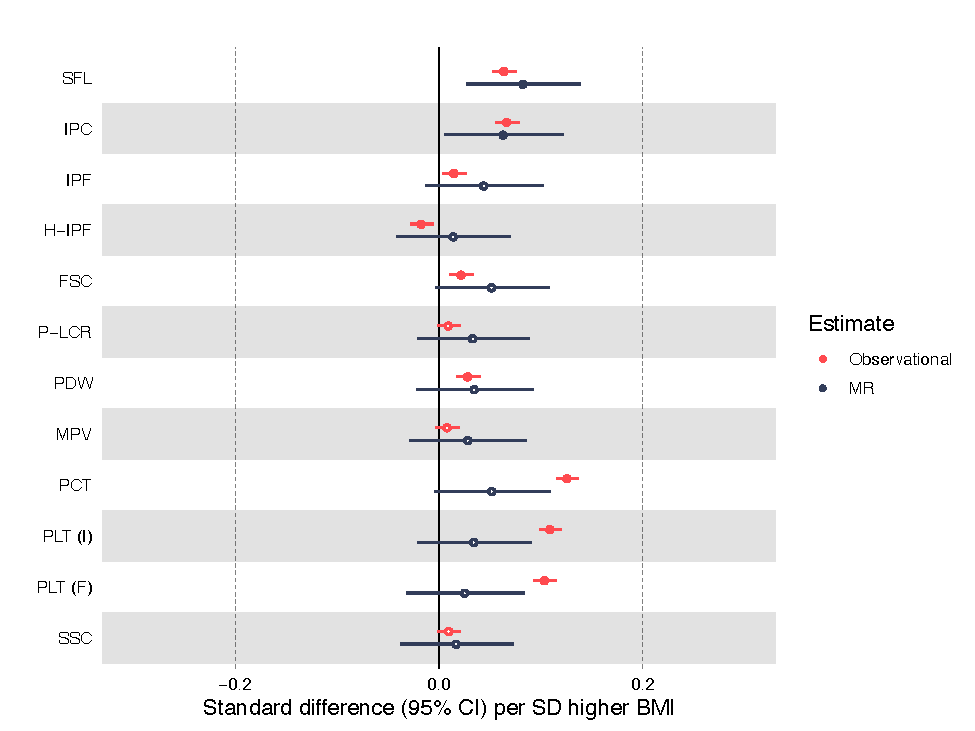
\includegraphics[width=0.9\linewidth]{figure/BMI_platelets/BMI_platelet_forestplot} 

}

\caption[Forest plot of the Mendelian randomization and unadjusted observational estimates for the effect of BMI on platelet traits]{\textbf{Forest plot of the Mendelian randomization (MR) and unadjusted observational estimates for the effect of BMI on platelet traits.} Estimate points are filled where P \textless{} 0.05. SFL = side fluorescence, IPC = immature platelet count, H-IPF = high fluorescence immature platelet function, FSC = forward scatter, P-LCR = platelet large cell ratio, PDW = platelet distribution width, MPV = mean platelet volume, PCT = plateletcrit, PLT (I) = platelet count (impedance channel), PLT (F) = platelet count (PLT-F channel), SSC = side scatter.}\label{fig:BMI-platelet-forest}
\end{figure}
\hypertarget{stratifying-bmi-and-ipc-associations-by-bmi-group}{%
\subsection{Stratifying BMI and IPC associations by BMI group}\label{stratifying-bmi-and-ipc-associations-by-bmi-group}}

We explored whether associations between BMI and IPC varied across NHS BMI groups (underweight \textless18.5 kg/m\textsuperscript{2}, healthy weight 18.5-24.9kg/m\textsuperscript{2}, overweight 25-29.9 kg/m\textsuperscript{2}, obesity 30+ kg/m\textsuperscript{2}). IPC had consistent BMI effects across observational and MR analyses. Stratifying by BMI category suggested that the strongest association between BMI and IPC was the overweight category (Table \ref{tab:BMI-platelets-stratified}).

\blandscape




\begin{longtable}[]{@{}
  >{\raggedright\arraybackslash}p{(\columnwidth - 20\tabcolsep) * \real{0.13}}
  >{\raggedright\arraybackslash}p{(\columnwidth - 20\tabcolsep) * \real{0.11}}
  >{\raggedright\arraybackslash}p{(\columnwidth - 20\tabcolsep) * \real{0.09}}
  >{\raggedright\arraybackslash}p{(\columnwidth - 20\tabcolsep) * \real{0.05}}
  >{\raggedright\arraybackslash}p{(\columnwidth - 20\tabcolsep) * \real{0.15}}
  >{\raggedright\arraybackslash}p{(\columnwidth - 20\tabcolsep) * \real{0.05}}
  >{\raggedright\arraybackslash}p{(\columnwidth - 20\tabcolsep) * \real{0.07}}
  >{\raggedright\arraybackslash}p{(\columnwidth - 20\tabcolsep) * \real{0.06}}
  >{\raggedright\arraybackslash}p{(\columnwidth - 20\tabcolsep) * \real{0.06}}
  >{\raggedright\arraybackslash}p{(\columnwidth - 20\tabcolsep) * \real{0.11}}
  >{\raggedright\arraybackslash}p{(\columnwidth - 20\tabcolsep) * \real{0.11}}@{}}
\caption{\label{tab:BMI-platelets-stratified}\textbf{Associations between BMI and immature platelet count (IPC) stratified by NHS BMI category.} Beta coefficient is the change in IPC (SDs) per SD increase in BMI}\tabularnewline
\toprule
Adjustment & Group & BMI range & N & Beta coefficient & SE & P value & R\textsuperscript{2} & 95\% CI & Lower 95\% CI & Upper 95\% CI \\
\midrule
\endfirsthead
\toprule
Adjustment & Group & BMI range & N & Beta coefficient & SE & P value & R\textsuperscript{2} & 95\% CI & Lower 95\% CI & Upper 95\% CI \\
\midrule
\endhead
Age and sex & Underweight & \textless18.5 & 169 & 0.202 & 0.834 & 0.461 & -0.009 & 1.635 & -1.434 & 1.837 \\
Age and sex & Healthy & 18.5-24.9 & 11889 & 0.039 & 0.018 & 0.026 & 0.003 & 0.035 & 0.005 & 0.074 \\
Age and sex & Overweight & 25-29.9 & 10189 & 0.092 & 0.034 & 0.006 & 0.006 & 0.066 & 0.027 & 0.158 \\
Age and sex & Obese & 30+ & 5008 & 0.032 & 0.032 & 0.315 & 0.004 & 0.063 & -0.031 & 0.096 \\
Fully adjusted & Underweight & \textless18.5 & 149 & 0.269 & 0.296 & 0.366 & 0.033 & 0.58 & -0.311 & 0.849 \\
Fully adjusted & Healthy & 18.5-24.9 & 10500 & 0.033 & 0.019 & 0.079 & 0.004 & 0.037 & -0.004 & 0.069 \\
Fully adjusted & Overweight & 25-29.9 & 8918 & 0.07 & 0.036 & 0.052 & 0.006 & 0.07 & 0 & 0.14 \\
Fully adjusted & Obese & 30+ & 4342 & 0.018 & 0.035 & 0.614 & 0.005 & 0.069 & -0.051 & 0.086 \\
\bottomrule
\end{longtable}
\elandscape

\hypertarget{follow-up-associations-between-ipc-and-whole-blood-aggregation-in-coptic}{%
\subsection{Follow-up associations between IPC and whole blood aggregation in COPTIC}\label{follow-up-associations-between-ipc-and-whole-blood-aggregation-in-coptic}}

Given evidence for a causal effect of BMI on IPC in the MR analysis, we sought to evaluate the relationship between IPC and platelet activity as a biological parameter of clinical relevance. Whilst this analysis could not be conducted in INTERVAL due to a lack of suitable data, we were able to utilize data from the COPTIC study to address this question. The COPTIC study is a cohort of cardiac surgery patients, with samples taken pre-surgery. These participants have whole blood aggregation measured, therefore making it possible to determine associations between IPC and aggregation in a clinical setting.

\hypertarget{coptic-participant-characteristics}{%
\subsection{COPTIC participant characteristics}\label{coptic-participant-characteristics}}

The total number of COPTIC participants was 2,541. Of these, 2,518 participants gave consent for future research (Table \ref{tab:COPTIC-participants-platelets}). Participants included in the analysis were those not on antiplatelet therapy (N=655). The majority of participants were male (61.8\%), with a mean age of 63.9 years (SD of 16.1). Similar to the INTERVAL cohort, the mean BMI was in the overweight category (27.2 kg/m\textsuperscript{2} with a SD of 4.9 kg/m\textsuperscript{2}). The majority of participants were either never smokers or ex-smokers for more than 5 years (89.2 \%). The effect estimate for the effect of BMI on IPC was 0.06 (95\% CI -0.01 to 0.14, P=0.09) and therefore consistent with that estimated in the INTERVAL cohort (Table \ref{tab:BMI-platelets-COPTIC}).




\begin{table}

\caption[Characteristics of COPTIC study participants]{\label{tab:COPTIC-participants-platelets}\textbf{Characteristics of COPTIC study participants}}
\centering
\begin{tabu} to \linewidth {>{\raggedright\arraybackslash}p{4cm}>{\raggedright}X>{\raggedleft}X>{\raggedright}X>{\raggedleft}X}
\toprule
Variable & Mean (SD) or \% (all) & N (all) & Mean (SD) or \% (included) & N (included)\\
\midrule
Age & 66.7 (11.9) & 2502 & 63.9 (16.1) & 655\\
Sex &  & 2518 &  & 655\\
\hspace{1em}Female & 24.9 \% &  & 38.2 \% & \\
\hspace{1em}Male & 75.1 \% &  & 61.8 \% & \\
Body mass index (kg/m2) & 27.9 (4.6) & 2422 & 27.2 (4.9) & 649\\
\addlinespace
Smoking &  & 2469 &  & 654\\
\hspace{1em}Never & 38.5 \% &  & 50.8 \% & \\
\hspace{1em}Ex-smoker (>5 years) & 47.4 \% &  & 38.4 \% & \\
\hspace{1em}Ex-smoker (1-5 years) & 8.3 \% &  & 6.3 \% & \\
\hspace{1em}Ex-smoker (30 days to 1 year) & 1.9 \% &  & 2.1 \% & \\
\addlinespace
\hspace{1em}Current smoker & 3.9 \% &  & 2.4 \% & \\
Antiplatelet medications &  & 2467 &  & 655\\
\hspace{1em}0 & 26.6 \% &  & 100 \% & \\
\hspace{1em}1 & 50.7 \% &  &  & \\
\hspace{1em}2 & 22.5 \% &  &  & \\
\addlinespace
\hspace{1em}3 & 0.2 \% &  &  & \\
ADP aggregation (AU) & 138.2 (50.1) & 2377 & 141 (46.5) & 625\\
Adrenaline aggregation (AU) & 53.0 (28.2) & 2363 & 56.8 (32.3) & 621\\
Arachidonic acid aggregation (AU) & 86.9 (62.1) & 2375 & 148.9 (52.4) & 623\\
TRAP-6 aggregation (AU) & 200.0 (50.1) & 2373 & 198.7 (50.0) & 623\\
\addlinespace
Platelet count (x 10E9 /L) & 209.8 (60.5) & 2409 & 200.9 (57.6) & 637\\
Mean platelet volume (fL) & 10.6 (1.0) & 2400 & 10.6 (0.98) & 634\\
Immature platelet fraction (\%) & 3.2 (1.9) & 2379 & 3.3 (2.0) & 628\\
Immature platelet count (x 10E9/L) & 6.3 (3.4) & 2383 & 6.2 (3.3) & 629\\
\bottomrule
\end{tabu}
\end{table}
\blandscape




\begin{longtable}[]{@{}lllllllll@{}}
\caption{\label{tab:BMI-platelets-COPTIC}\textbf{Association between BMI and platelet parameters in COPTIC (adjusted for age, sex, smoking).} Beta coefficient is the change in platelet measure ins SDs per SD higher BMI.}\tabularnewline
\toprule
Outcome & N & Beta coefficient & SE & P value & R\textsuperscript{2} & 95\% CI & Lower 95\% CI & Upper 95\% CI \\
\midrule
\endfirsthead
\toprule
Outcome & N & Beta coefficient & SE & P value & R\textsuperscript{2} & 95\% CI & Lower 95\% CI & Upper 95\% CI \\
\midrule
\endhead
MPV & 627 & 0.08 & 0.04 & 0.04 & 0.003 & 0.07 & 0.00 & 0.15 \\
IPC & 622 & 0.06 & 0.04 & 0.09 & 0.013 & 0.07 & -0.01 & 0.14 \\
PLT & 630 & 0.04 & 0.04 & 0.32 & 0.071 & 0.07 & -0.03 & 0.1 \\
IPF & 621 & 0.03 & 0.04 & 0.36 & 0.014 & 0.07 & -0.04 & 0.11 \\
\bottomrule
\end{longtable}
\elandscape

\hypertarget{association-between-ipc-and-aggregation-in-coptic-cohort}{%
\subsection{Association between IPC and aggregation in COPTIC cohort}\label{association-between-ipc-and-aggregation-in-coptic-cohort}}

To determine the potential functional effects of variation in IPC, the COPTIC cohort was used to assess the observational association between IPC and whole blood platelet aggregation in response to a range of platelet agonists (Figure \ref{fig:IPC-aggregation}A). In participants who were not on antiplatelet therapy (up to N=655), there was evidence for a positive association between IPC and aggregation induced by adrenaline (0.13 SD increase per SD increase in IPC, 95\% CI 0.04 to 0.21, p=3.7x10\textsuperscript{-3}), TRAP-6 (0.11 SD increase per SD increase in IPC, 95\% 0.03 to 0.18, p=7.8x10\textsuperscript{-3}) and ADP (0.08 SD per SD increase in IPC, 95\% 0.01 to 0.0.15, p=0.04). As there was a high correlation among platelet traits (Figure \ref{fig:IPC-aggregation}A, Figure \ref{fig:IPC-aggregation}B), the effect of MPV, PLT and IPF were also assessed. PLT was associated with all four measures of aggregation, with a larger effect estimate than IPC (Figure \ref{fig:IPC-aggregation}A). The finding that IPC does not correlate with PLT however suggests that the effect of IPC on platelet aggregation is independent of the effect of PLT on platelet aggregation (Figure \ref{fig:IPC-aggregation}B). Fitting PLT alongside IPC as an additional predictor of aggregation had little effect on the IPC effect estimate providing further evidence of independent contributions from the two traits (Figure \ref{fig:IPC-aggregation}C). Adjustment for PLT in the regression model for the association between IPF and aggregation provided estimates of a similar magnitude to that of IPC and aggregation.




\begin{figure}

{\centering 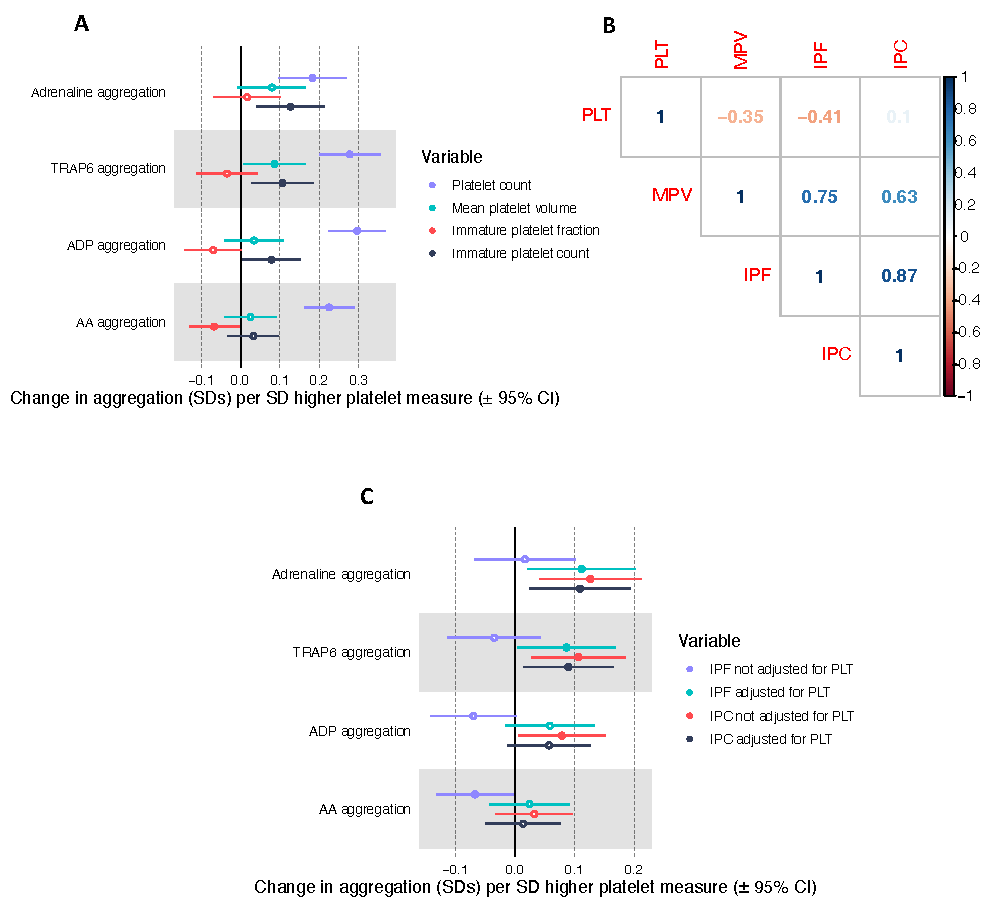
\includegraphics[width=0.85\linewidth]{figure/BMI_platelets/IPC_aggregation} 

}

\caption[Association between platelet measures and whole blood platelet aggregation in COPTIC trial participants]{\textbf{Association between platelet measures and whole blood platelet aggregation in COPTIC trial participants.} A) Forest plot displaying the association between platelet measures (exposure) and aggregation (outcomes). B) Correlation matrix displaying the Pearson's correlation coefficient (r) between platelet traits. C) Forest plot displaying the effect estimate for the association between immature platelet count (IPC) or immature platelet fraction (IPF) and measures of aggregation, with or without adjustment for platelet count (PLT). ADP = adenosine diphosphate, AA = arachidonic acid, MPV = mean platelet volume.}\label{fig:IPC-aggregation}
\end{figure}
\hypertarget{discussion}{%
\section{Discussion}\label{discussion}}

In this study we used data from 33,388 healthy blood donors to study the effect of BMI on platelet phenotypes including measures of count, size and maturity. The combination of observational and MR estimates suggested a positive causal effect of BMI on SFL and IPC. The observational analysis revealed a strong association between BMI and both PLT and PCT, however the MR estimates did not provide evidence to support this association as causal. Observational analysis using data from a cardiac surgery cohort provided evidence for a positive association between IPC and aggregation induced by adrenaline, TRAP6 and ADP. A summary of these findings is indicated in \ref{fig:BMI-platelet-cartoon}.


\begin{figure}
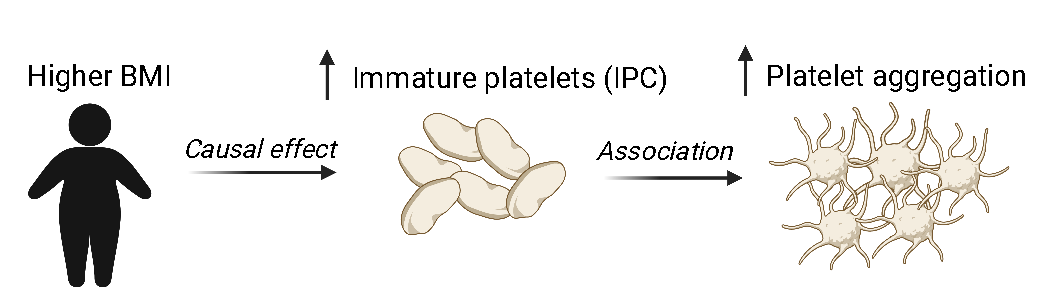
\includegraphics[width=0.9\linewidth]{figure/BMI_platelets/Visual_abstract} \caption{Graphical summary of findings}\label{fig:BMI-platelet-cartoon}
\end{figure}
The observational and MR analyses in the current study provide evidence for a positive association between BMI and both IPC and SFL. Stratifying by NHS BMI category suggested that this estimate is strongest in the overweight category. As IPC is derived using SFL, the measure of mRNA content, these measures are highly correlated. Whilst few studies have explored the direct association between BMI and immature platelet measures, there is some evidence for increased immature platelets in subjects with metabolic syndrome (MS) and subjects with type II diabetes compared with control subjects\textsuperscript{\protect\hyperlink{ref-Vaduganathan2008a}{103},\protect\hyperlink{ref-Mijovic2015a}{104}}. In these studies, participants with MS or type II diabetes also had a higher BMI, which could be a possible cause of this increase in immature platelets. Indeed, evidence from our analysis suggests that BMI, independent of metabolic syndrome or type II diabetes, may causally influence IPC and SFL.

As IPC is an indirect measure of platelet production\textsuperscript{\protect\hyperlink{ref-Lev2016a}{100}}, these results suggest that an increased BMI may lead to an increased production of platelets. It has been reported that immature platelets have increased thrombotic potential\textsuperscript{\protect\hyperlink{ref-Lev2016a}{100},\protect\hyperlink{ref-Grove2011a}{112}} and may be predictive of cardiovascular events\textsuperscript{\protect\hyperlink{ref-Freynhofer2017a}{43},\protect\hyperlink{ref-Ibrahim2014}{72}}, suggesting that an increase in the number of immature platelets may be of functional and clinical relevance. A follow-up analysis confirmed that higher IPC was associated with greater platelet aggregation independent of absolute platelet count within a cardiac surgery cohort. Positive associations were found between IPC and aggregation induced by adrenaline, TRAP-6 and ADP, suggesting general platelet hyperactivity with more immature platelets. A previous study in a coronary artery disease cohort also found a positive correlation between IPC and aggregation induced by arachidonic acid, collagen and ADP\textsuperscript{\protect\hyperlink{ref-Grove2011a}{112}}. These findings suggest that IPC can be used as a proxy for platelet hyperactivity within a cohort with a history of cardiovascular disease. Measures of immature platelets are currently not considered in the clinic when prescribing antiplatelet therapy, however if a higher immature platelet count is demonstrative of newly produced, hyperactive platelets then this could be important in guiding dosage regimes to ensure sufficient platelet inhibition\textsuperscript{\protect\hyperlink{ref-Bernlochner2015a}{101}}. Observational studies have also found that patients with COVID-19 have elevated immature platelet counts and fraction, which could partly explain high rates COVID-19 induced thrombosis\textsuperscript{\protect\hyperlink{ref-Klok2020}{114}}. Despite the association between BMI and IPC, there was less evidence for an effect of BMI on IPF. This lack of association may be because IPF is the proportion of immature platelets, therefore if someone had a higher number of immature platelets, but also a higher number of platelets overall (for example due to increased platelet lifespan), there would be no increase in the immature platelet fraction.

In general, previous studies have reported positive observational associations between BMI and both PLT and PCT\textsuperscript{\protect\hyperlink{ref-Furuncuoglu2016}{67}}. More direct measures of body fat such as total fat mass, waist-hip ratio and waist circumference have also been reported to be positively associated with both PLT and PCT\textsuperscript{\protect\hyperlink{ref-Han2018a}{68}}; the observational evidence from the current study is in agreement with this. The MR analysis did not detect causal effects of BMI on measures of PLT/PCT, however the estimates were consistently positive. It is possible that IPC could be raised in absence of raised PLT as platelets may being produced at an increased rate, but could also be being destroyed at an increased rate. The small P values in the Wu-Hausman test for endogeneity for plateletcrit and platelet count variables support that the observational and MR estimates are different. Estimates could be biased due to confounding factors, reverse causation or other sources of bias. Possible routes of confounding could include stress, inflammation and nutrition, which could exert independent effects on both BMI and platelet count.

Both observational and MR estimates suggested that BMI is not associated with measures of platelet size, such as MPV and P-LCR. There are conflicting findings in the literature, with some studies suggesting that there is a positive association between BMI and MPV\textsuperscript{\protect\hyperlink{ref-Coban2005}{69}} and others showing no association\textsuperscript{\protect\hyperlink{ref-Furuncuoglu2016}{67},\protect\hyperlink{ref-Han2018a}{68},\protect\hyperlink{ref-Heffron2018}{70}}. The results of the current study suggest that associations seen previously between BMI and MPV are likely due to confounding of observational estimates. The lack of association between BMI and MPV may be surprising given a correlation coefficient of 0.62 between IPC and MPV. As BMI was positively associated with immature platelet count, and immature platelets tend to be larger, it may be surprising that BMI was not associated with measures of platelet size. However, immature platelets make up a small percentage of overall platelets (\textasciitilde3-6 \%)\textsuperscript{\protect\hyperlink{ref-Ibrahim2014}{72},\protect\hyperlink{ref-Bernlochner2015a}{101}}, therefore the increase in immature platelets may not affect the overall median size of the whole platelet population.

Although this study suggests potential effects of BMI on platelet traits such as SFL and IPC, it does not provide mechanistic insight into how BMI exerts these effects. Previous studies have suggested that inflammation driven by adiposity can stimulate megakaryocyte proliferation, thereby increasing platelet numbers\textsuperscript{\protect\hyperlink{ref-Han2018a}{68}}. There is evidence that inflammatory mediators such as interleukin-6 (IL-6) could be one such factor\textsuperscript{\protect\hyperlink{ref-Kaser2001}{115}}. Further study would be warranted to explore these mechanisms, as well as replicate the current findings, such as through independent population or clinical studies.

\hypertarget{INTERVAL-limitations}{%
\subsection{Limitations}\label{INTERVAL-limitations}}

There are a few limitations to the study that should be recognised. Firstly, BMI was derived from self-reported height and weight. Although there is potential for this to bias observations, previous studies have found that self-reported BMI and BMI measured in the clinic are strongly associated\textsuperscript{\protect\hyperlink{ref-Nikolaou2017}{116}}. The GRS also associates with BMI to the extent expected. Secondly, there may be other confounders which were not recorded within INTERVAL and therefore could not be accounted for in our models, such as, socio-economic position, which may affect both BMI and risk of thrombosis. Therefore, residual confounding of observational estimates cannot be ruled out. Whilst the INTERVAL study provided relatively precise estimates of effect overall, larger sample sizes within each BMI category would be required to further investigate potential nonlinearity in the relationship between BMI and IPC. With respect to the observational analysis conducted in COPTIC, the sample size is modest, which may limit power to detect associations. Furthermore, this cohort required cardiac surgery and therefore it is possible that associations found may not be generalizable to the wider population, as participants also displayed greater aggregatory responses than the reference ranges\textsuperscript{\protect\hyperlink{ref-Marcucci2015}{117}}. However, these findings do indicate that immature platelets may be a biomarker of platelet hyperactivity in patients with a history of cardiovascular disease. It is important to note that the anticoagulant used (EDTA) has been reported to affect platelet parameters, such as increasing MPV and decreasing PLT\textsuperscript{\protect\hyperlink{ref-Mannuuxdf2020}{118}}. Despite this, EDTA is the standard anticoagulant used for full blood counts in the NHS. The Sysmex analyzers used in INTERVAL and COPTIC were different models, however, it has been shown that there is strong association between platelet measures between the XE and newer XN analyzers\textsuperscript{\protect\hyperlink{ref-Briggs2012}{119}}.

Altogether, we show observational and MR evidence that an increased BMI is associated with an increase in number of immature platelets. Observational evidence indicates that higher immature platelet count is associated with enhanced aggregation in a cardiac surgery cohort. Together, these results indicate that higher BMI may enhance platelet function and thrombosis by increasing platelet production and immature platelet count.

\hypertarget{BMI-platelets-clinic}{%
\chapter{The effect of obesity on platelet function: a clinical pilot study}\label{BMI-platelets-clinic}}

The following chapter reports a specifically designed patient study. Recruitment into this study has been severely affected by the pandemic as approvals were set in place to start recruitment in March 2020. Further details of the initial plans for this study are provided in the discussion chapter (Chapter \ref{Discussion}). The platelet-neutrophil assay data was performed by Dr Chris Williams and the Sysmex haematology analyzer data was collected by Dr Kate Burley. Help was required here due to time constraints when receiving patient samples. Proteomic data were generated by Dr Marieangela Wilson and Dr Kate Heesom at the Proteomics facility at the University of Bristol. Analytical support was provided by Dr Phil Lewis from the Proteomics facility. Optimised methods have been used within a study to explore the effect of COVID-19 on platelet function given the increased risk of thrombosis. The COVID-19 research has been written up as a manuscript but it has not been included in the thesis due to not aligning with the current aims.

\hypertarget{background-2}{%
\section{Background}\label{background-2}}

As detailed in Chapter \ref{BMI-platelets-INTERVAL}, there is evidence that people with a higher BMI have an increased risk of cardiovascular events such as coronary heart disease (CHD) or stroke\textsuperscript{\protect\hyperlink{ref-Nordestgaard2012}{11},\protect\hyperlink{ref-Dale2017}{28},\protect\hyperlink{ref-Wolk2003a}{97}}. As platelets are one of the key cells involved in haemostasis and thrombosis\textsuperscript{\protect\hyperlink{ref-Koupenova2017a}{25}}, it is likely that a higher BMI has a direct effect on platelet function. The previous chapter provided evidence that higher BMI causes an increase in the production of immature platelets, evidenced by an increase in immature platelet count (IPC). IPC was also positively associated with whole blood platelet aggregation in response to various platelet agonists (adrenaline, protease activating receptor 1 peptide (PAR1-AP/TRAP-6) and adenosine diphosphate (ADP)) in a cardiac surgery cohort. Although these analyses suggest that higher BMI leads to platelet hyperactivity, this association was not directly assessed due to the limited platelet function data available. In COPTIC, the only available platelet function data was whole blood platelet aggregation; there are other platelet function assays which may provide more extensive information about platelet activation. COPTIC was also a cohort which had a history of cardiovascular disease, therefore associations could be confounded by the presence of cardiovascular disease. Therefore, studies which have information about body composition and detailed platelet function assays are required.

When an individual struggles with maintaining weight loss and there is concern for their health, bariatric surgery is advised. This surgery utilises various techniques (gastric band, bypass or sleeve) that aim to restrict the size of the stomach, therefore reducing appetite. Current NHS guidelines for bariatric surgery indicate that surgery is available for those with a BMI of 40+ kg/m\textsuperscript{2}. A BMI of over 40kg/m\textsuperscript{2} is current classified as having severe obesity. This group of patients is therefore a suitable patient group to obtain blood samples from in order to further characterise effects of a sustained high BMI.

Previous studies have attempted to determine the direct effects of BMI on platelet function and signalling, where there is conflicting evidence regarding how BMI affects platelet function\textsuperscript{\protect\hyperlink{ref-Nardin2015}{44},\protect\hyperlink{ref-Deharo2014}{49},\protect\hyperlink{ref-Sibbing2007}{50},\protect\hyperlink{ref-Barrachina2019}{99}}. Such studies have focused on the relationship between BMI and platelet function in patients receiving dual antiplatelet therapy (DAPT). In these studies there is evidence that in people with higher BMI, antiplatelet drugs such as prasugrel, which acts at the P2Y\textsubscript{12} receptor, may not be as effective at suppressing platelet activity\textsuperscript{\protect\hyperlink{ref-Deharo2014}{49}}. These findings have come from using a phospho-VASP assay. PGE1 suppresses platelet function by acting at a G\textsubscript{s} coupled receptor, resulting in activation of adenylate cyclase and a rise in cAMP, subsequent activation of PKA and phosphorylation of VASP. G\textsubscript{i/o} coupled GPCRs oppose G\textsubscript{s} pathways: activation of the ADP receptor P2Y\textsubscript{12} receptor inhibits activation of adenylate cyclase through G\textsubscript{i/o} thereby opposing PGE1-mediatied VASP phosphorylation. Lower phospho-VASP levels are therefore indicative of less inhibition by the antiplatelet drug and more activation of the platelet by ADP. It is less clear what the relationship is between BMI and platelet function in those who are not on any antiplatelet therapy and across other platelet function assays. In this study I therefore aimed to determine whether high BMI is associated with an alteration in platelet function and signalling (Figure \ref{fig:BMI-platelet-overview2}).



\begin{figure}

{\centering \includegraphics[width=0.9\linewidth]{figure/Bariatric_study/Thesis_graphic_overview_BMI_platelets} 

}

\caption[Schematic of the associations explored in the current chapter]{\textbf{Schematic of the associations explored: this chapter explores the relationship between body mass index and platelet function.} Figure made using BioRender.com.}\label{fig:BMI-platelet-overview2}
\end{figure}
\hypertarget{materials-and-methods}{%
\section{Materials and Methods}\label{materials-and-methods}}

\hypertarget{materials}{%
\subsection{Materials}\label{materials}}

Protease-activated receptor 1 (PAR-1)-activating peptide (TRAP-6/SFLLRN-NH2) was from Bachem (Bubendorf, Switzerland), crosslinked collagen-related peptide (CRP-XL) from Prof.~Richard Farndale (Department of Biochemistry, University of Cambridge, UK). Adenosine diphosphate (ADP) was from Sigma-Aldrich (Poole, UK). cOmplete mini protease inhibitor tablets and phosSTOP phosphatase inhibitors were from Roche Life Sciences (Welwyn Garden City, UK). The Pierce bicinchoninic acid (BCA) assay was from ThermoFisher Scientific (Altrincham, UK). Sodium Citrate Vacutainer® tubes, FixLyse, PE-Cy5-conjugated mouse anti-human CD42b antibody, FITC mouse anti-human CD61 antibody, Fc block, PE mouse anti-human platelet GPVI antibody, FITC mouse anti-human PAC-1 and PE mouse anti-human CD62P antibodies were from BD (Wokingham, UK). FITC mouse anti-human CD41 and CD42b antibodies were from BioLegend (London, UK). Human MDC (69 amino acids) and TARC were from PeproTech (London, UK). Indomethacin, PGE1, Triton X-100, apyrase, HEPES Tyrode's (10 mM HEPES, 1 mM magnesium, 0.5 mM monosodium phosphate, 145 mM sodium chloride, 3 mM potassium chloride, pH 7.2), 2-butanol, ethanol, methanol and bovine serum albumin (BSA) were purchased from Sigma-Aldridge (Poole, UK). Phosphate buffered saline (PBS), trisodium citrate, acid citrate dextrose (ACD), D-glucose, ammonium persulfate (APS), Tris buffered saline (TBS), polysorbate 20 (Tween 20), Donkey anti-Rabbit IgG (H+L) Highly Cross Adsorbed Secondary Antibody Alexa Fluor 647 and Fura-2 were purchased from Thermo Fisher Scientific (Loughborough, UK). 30 \% acrylamide mix (37.5:1), 1.0 M Tris pH 6.8 solution and 1.5 M Tris pH 8.8 solution purchased from National Diagnostics (Nottingham, UK). Immobilon-FL PVDF membranes (0.45-micron filter) were purchased from Merck Millipore (Hertfordshire, UK). Sodium dodecyl sulphate (SDS) was purchased from GE Healthcare worldwide (Hatfield, UK). SDS solution (10 \%), tetramethylethylenediamine (TEMED), filter paper and Precision Plus protein pre-stained standards were purchased from Bio-Rad laboratories (Bredbury, UK). Blocking buffer was purchased from LI-COR Biosciences (Cambridge, UK). Rabbit pSer239 VASP and pSer157 VASP antibodies and pSer425 Talin were purchased from Cell Signaling Technology (Hertfordshire, UK). Alexa Fluor 680 AffiniPure Donkey Anti-Goat IgG and Alexa Fluor 680 AffiniPure Donkey Anti-Rabbit IgG were obtained from Jackson Immunoresearch (Cambridgeshire, UK). Paraformaldehyde was purchased from Acros Organics (Geel, Belgium). Annexin V Alexa Fluor 568 conjugate was from ThermoFisher. The inhibitor AZD-2908 was from Bio-Techne, YM-284890 was from Tebu-Bio Ltd and Y27632 was from Generon Ltd.~Tween-20 (Sigma G02062) and hyrogenated gelatine (Sigma P1379) were from Sigma-Aldrich (Poole, UK).

\hypertarget{ethical-approval-process}{%
\subsection{Ethical approval process}\label{ethical-approval-process}}

This study was designed in July 2019. To be able to carry out a patient study, there were various documents that needed to be prepared. These were submitted using the Integrated Research Application System (IRAS). Documents included were a research protocol, statistical review, IRAS form, consent forms and participant information sheets for bariatric patients and control subjects, GP letters and a copy of the email invite sent out to control participants. Upon ethical approval from the London Riverside Research Ethics Committee (REC reference 19/LO/1781) and approval from Southmead Hospital, this study was first approved to start recruitment in March 2020. Recruitment was put on hold until May 2021 due to the pandemic. During this time, two amendments were made to be able to account for: 1) whether the participant had previously had a COVID-19 infection and 2) whether the participant had been vaccinated for COVID-19 due to reports that COVID-19 infection and the AstraZeneca vaccine lead to an increased risk of thrombotic outcomes\textsuperscript{\protect\hyperlink{ref-Middeldorp2020}{120},\protect\hyperlink{ref-Scully2021}{121}}. The second amendment was not approved by Southmead Hospital in time and therefore the vaccination status could not be recorded for bariatric patients.

\hypertarget{study-population-1}{%
\subsection{Study population}\label{study-population-1}}

All participants provided written informed consent. Patients, who were due to undergo bariatric surgery, with a body mass index of \textgreater40kg/m\textsuperscript{2}, were recruited from the Department of Bariatric and Metabolic Surgery at Southmead Hospital, Bristol. Control participants with a BMI between 18.5 and 25 kg/m\textsuperscript{2} were recruited from the University of Bristol. Inclusion criteria for participants were: aged 18 years and over, able to give written informed consent and sufficient level of English to understand the study and ask any questions. Participants were excluded if they were pregnant or lactating, had any known clotting or bleeding disorders (e.g.~von Willebrand disease or drug-induced thrombocytopenia), or if they had taken any antiplatelet medication within the previous 14 days such as clopidogrel, ticagrelor or aspirin or any other non-steroidal anti-inflammatory drug (NSAID). Recruitment occurred between May 2021 and June 2021. As a pilot study, a total of four bariatric patients with obesity and four age and sex-matched control participants were recruited. Bariatric patients donated blood before bariatric surgery.

\hypertarget{isolation-of-platelet-rich-plasma-prp}{%
\subsection{Isolation of platelet rich plasma (PRP)}\label{isolation-of-platelet-rich-plasma-prp}}

Blood was taken by venipuncture into vacutainers containing sodium citrate (3.2\%). Blood was centrifuged (1000 RPM, 17 mins). PRP was diluted 1:40 in HEPES Tyrode's (145 mM NaCl, 3 mM KCl, 0.5 mM Na\textsubscript{2}HPO\textsubscript{4}, 1 mM MgS0\textsubscript{4}.7H\textsubscript{2}O, 10 mM HEPES, pH 7.4, 0.1\% {[}w/v{]} D‐glucose) for experiments where indicated.

\hypertarget{platelet-lysates}{%
\subsection{Platelet lysates}\label{platelet-lysates}}

ACD (1:7) and apyrase (0.02 U/mL) were added to PRP. PRP was centrifuged (1700 RPM, 10 mins) to pellet platelets. Platelets were resuspended in CGS buffer (120 mM NaCl, 25.8 mM sodium citrate dihydrate, 0.1\% {[}w/v{]} D‐glucose, 0.02 U/mL apyrase, pH 6.5) Platelets were centrifuged again (1700 RPM, 10 mins) to pellet platelets and were resuspended in CGS buffer. Platelets were pelleted and resuspended in radioimmunoprecipitation assay buffer (RIPA: 25 mM HEPES, 200 mM NaCL, 1mM EDTA, 1 \% (v/v) NP40, 0.5 \% (w/v) sodium deoxychelate, 0.1 \% (w/v) SDS) supplemented with a protease and phosphatase inhibitor for 10 minutes on ice. Lysates were centrifuged (10000 RPM, 4°C for 5 minutes). Supernatant was removed and a bicinchoninic acid (BCA) assay was performed to calculate sample protein concentrations. Samples were stored in a -80°C freezer until proteomics analysis.

\hypertarget{platelet-parameters-measured-by-sysmex}{%
\subsection{Platelet parameters measured by Sysmex}\label{platelet-parameters-measured-by-sysmex}}

Citrated whole blood (200 uL) was analysed using the Sysmex XN-20 haematology analyser. Platelet readouts were platelet count (PLT) (x 10\textsuperscript{9}/L), immature platelet fraction (IPF) (\%), immature platelet count (IPC) (x 10\textsuperscript{9}/L), side fluorescence (SFL, a measure of mRNA content in relative fluorescent units/RFUs), forward scatter (FSC, a measure of platelet size measured in RFUs) and side scatter (SSC, a measure of granularity in RFUs).

\hypertarget{freeze-dried-agonist-plates}{%
\subsection{Freeze-dried agonist plates}\label{freeze-dried-agonist-plates}}

Agonist was freeze dried onto plates to reduce day-to-day variation in agonist concentrations, as described previously.\textsuperscript{\protect\hyperlink{ref-Chan2018}{53}} 96 well plates were coated with 10 mM PBS with 0.75\% w/v hydrogenated gelatine and 0.05\% v/v Tween-20 with a pH of 0.74 and left for 4 hours at room temperature. Plates were washed with dH\textsubscript{2}O with 0.01\% v/v Triton X-100, followed by two washes with dH\textsubscript{2}O and left to dry in a fume hood. Agonist was added to the plates (5uL per well at 10x final concentration): agonists used were protease-activated receptor 1 activating protein (PAR1-AP), adenosine diphosphate (ADP) and collagen related peptide (CRP). Plates were then stored in a -80°C freezer for 1 hour, then placed into the freeze dryer (-50°C) and left overnight. Once freeze-dried, plates were vacuum packed.

\hypertarget{integrin-ux3b1iibux3b23-activation-and-p-selectin-expression-measured-by-flow-cytometry}{%
\subsection{\texorpdfstring{Integrin α\textsubscript{IIb}β\textsubscript{3} activation and P-selectin expression measured by flow cytometry}{Integrin αIIbβ3 activation and P-selectin expression measured by flow cytometry}}\label{integrin-ux3b1iibux3b23-activation-and-p-selectin-expression-measured-by-flow-cytometry}}

Isolated PRP was diluted 1:40 in HEPES Tyrode's. FITC-conjugated PAC1 and PE-conjugated CD62P antibodies were added in a 2:1 ratio (5uL PAC1 and 2.5uL CD62P per well). This master mix was added to pre-prepared vacuum packed 96 well plates with freeze-dried agonist to a final folume of 50 uL. HEPES Tyrode's was also freeze-dried onto plates, which was used for a measurement of unstimulated integrin α\textsubscript{IIb}β\textsubscript{3} activation and P-selectin expression. Platelets were stimulated with agonists for 10 minutes. Platelets were fixed with 1\% paraformaldehyde (PFA) for 10 minutes. Platelets were gated and the median fluorescence intensity (MFI) in arbitrary units (AUs) was reported from a total of 10,000 events.

\hypertarget{surface-receptor-levels-measured-by-flow-cytometry}{%
\subsection{Surface receptor levels measured by flow cytometry}\label{surface-receptor-levels-measured-by-flow-cytometry}}

Diluted PRP (1:40) was used for unstimulated surface receptor detection. Antibodies were added (1:10 v/v) to a final volume of 50 uL. Antibodies used include anti-human CD41 (α\textsubscript{IIb}), CD42b (GP1bα), CD61 (β\textsubscript{3}) (FITC-conjugated) and GPVI and CD110 (thrombopoietin/TPO receptor) (PE-conjugated). Platelets were fixed with 1\% PFA for 10 minutes. Platelets were gated and the MFI was reported in AUs from a total of 10,000 events.

\hypertarget{platelet-neutrophil-assay-measured-by-flow-cytometry}{%
\subsection{Platelet-neutrophil assay measured by flow cytometry}\label{platelet-neutrophil-assay-measured-by-flow-cytometry}}

Citrated whole blood was diluted 1:10 in HEPES-Tyrode's buffer and incubated with FITC-conjugated anti-CD41 and PE-conjugated anti-C45 antibodies at room temperature for 15 mins (antibodies used 1:10 v/v). Samples were either stimulated (+ 5 ug/mL CRP) or unstimulated (+ vehicle) for the same 15 minute duration. Samples were fixed with FixLyse for 10 minutes, followed by a final concentration of 4 \% PFA for 10 minutes. Fluorescence was quantified using the flow cytometer, where 1000 neutrophil events were analysed based on a gating of CD45 and SSC parameters. Aggregates of platelets and neutrophils were defined by being both CD41+ and CD45+.

\hypertarget{tandem-mass-tag-mass-spectrometry-tmt-ms-quantification-of-platelet-proteins}{%
\subsection{Tandem Mass Tag Mass Spectrometry (TMT-MS) quantification of platelet proteins}\label{tandem-mass-tag-mass-spectrometry-tmt-ms-quantification-of-platelet-proteins}}

Platelet lysate samples (50 ug total protein) were digested with trypsin and labelled with TMT 15 plex reagents (ThermoFisher Scientific, Loughborough, UK). Labelled samples were pooled. The pooled sample was evaporated to dryness then resuspended in formic acid (5\%). The pooled sample was then desalted using a SepPak cartridge (Waters, Milford, Massachussetts, USA). Eluate from the SepPak cartridge was evaporated to dryness and resuspended prior to fractionation by high pH reversed-phase chromatography using an Ultimate 3000 liquid chromatography system (Thermo Fisher Scientific). Further fractionation occurred using high pH RP fractions using the Ulitamte 3000 nano-LC system in line with an Orbitrap Fusion Tribrid Mass Spectrometer (ThermoFisher Scientific). Further details of the methods used for mass spectrometry within the proteomics facility have been previously published\textsuperscript{\protect\hyperlink{ref-Durrant2020}{122}}.

\hypertarget{statistical-analysis-for-platelet-function-assays}{%
\subsection{Statistical analysis for platelet function assays}\label{statistical-analysis-for-platelet-function-assays}}

Data was analysed using GraphPad Prism 8. All data points are presented where possible to be fully transparent. If data displayed a normal distribution (based on Shapiro-Wilk p-value and W statistic), a parametric test was used (e.g.~unpaired t-test or one way ANOVA), otherwise a nonparametric test was used. Concentration-response curves were plotted using a four parameter variable slope. To compare concentration-response curve parameters, pEC50s or curve maxes were compared. A Fisher's exact test was used to compare proportions of categorical variables. Statistical tests used for each experiment are provided in figure legends. P-values for results are presented throughout, however these were not dichotomised as either `significant' or `not significant'\textsuperscript{\protect\hyperlink{ref-Sterne2001}{123}} as the current study has low power and the groups are unlikely to be representative of the respective populations. A P-value threshold of 0.05 may therefore not be appropriate in this case.

\hypertarget{analysis-of-proteomic-data}{%
\subsection{Analysis of proteomic data}\label{analysis-of-proteomic-data}}

A principal component analysis (PCA) was performed to reduce the data and to identify major axes (principal components, PCs). This method helps to determine whether the major axes of the data can likely be explained by the group (bariatric patient with obesity or control participant). Normalised protein abundances were log\textsubscript{2} transformed, where the logFC was calculated by subtracting the log\textsubscript{2} normalised protein abundance of the control subjects from the bariatric surgery group. The log\textsubscript{2} normalised protein abundances of bariatric patients were compared to controls using a two-tailed unpaired t-test. P-values were not adjusted for multiple testing, due to the observation that false discovery rate (FDR) adjustment may be too blunt in low power proteomics experiments\textsuperscript{\protect\hyperlink{ref-Pascovici2016}{124}}. P-values of all comparisons are provided in the supplementary results in Chapter \ref{BMI-platelets-clinic}. (FDR) adjusted p-values are also provided in the full results as a reference. A positive logFC indicates an increase in protein level in the bariatric samples.

\hypertarget{results-1}{%
\section{Results}\label{results-1}}

\hypertarget{participant-characteristics}{%
\subsection{Participant characteristics}\label{participant-characteristics}}

The characteristics of participants included in the study are shown in Table \ref{tab:obesity-platelets-participants}. The mean BMI in the control group was 21.8 kg/m\textsuperscript{2} (SD 2.1 kg/m\textsuperscript{2}) and 49.3 kg/m\textsuperscript{2} (SD 8.8 kg/m\textsuperscript{2}). Participants in the control group and bariatric patient group were age and sex matched. All bariatric patients and control participants were non-smokers. Half of the bariatric patients presented with type 2 diabetes (T2D) and were receiving T2D medication, whereas none of the control participants had T2D. Similarly, 75\% of the bariatric patients had previously had a positive test for COVID-19 but none of the control participants had ever tested positive for COVID-19.



\begin{table}

\caption[Characteristics of included participants in the body mass index and platelet function study]{\label{tab:obesity-platelets-participants}\textbf{Characteristics of included participants in the body mass index and platelet function study}}
\centering
\begin{tabu} to \linewidth {>{\raggedright\arraybackslash}p{5cm}>{\raggedright}X>{\raggedright}X>{\raggedright}X}
\toprule
Variable & Control mean (SD) or \% & Bariatric patient mean (SD) or \% & P value for difference\\
\midrule
Age & 42.2 (14.1) & 46 (18.0) & 0.77\\
Sex & 75 \% & 75 \% & 1\\
Body mass index (kg/m2) & 21.8 (2.1) & 49.3 (8.8) & 9e-04\\
Smoker & 0 \% & 0 \% & 1\\
Hypertensive (140/90 mmHg) & 0 \% & 25 \% & 1\\
\addlinespace
Type 2 Diabetes & 0 \% & 50 \% & 0.43\\
Type 2 Diabetes medication & NA &  & NA\\
\hspace{1em}Metformin &  & 25 \% & \\
\hspace{1em}Dapagliflozin &  & 25 \% & \\
\hspace{1em}Dulaglutide &  & 25 \% & \\
\addlinespace
Previous COVID-19 infection & 0 \% & 75 \% & 0.14\\
\bottomrule
\end{tabu}
\end{table}
\hypertarget{platelet-parameters}{%
\subsection{Platelet parameters}\label{platelet-parameters}}

Platelet traits measured by Sysmex were compared across bariatric and control groups (Table \ref{tab:obesity-platelets-parameters}). There was no statistical evidence for an effect of obesity on platelet parameters. However, IPC and IPF did display larger mean values compared to controls, but they also had relatively large SDs in the bariatric patient group (IPC 9.3 (SD 4.9) x 10\textsuperscript{9}/L in control vs 16.3 (SD 16.3) x 10\textsuperscript{9}/L in bariatric group, p=0.45). The bariatric patient group displayed larger standard deviations than the control group for all platelet paramaters.

\blandscape



\begin{longtable}[]{@{}
  >{\raggedright\arraybackslash}p{(\columnwidth - 6\tabcolsep) * \real{0.37}}
  >{\raggedright\arraybackslash}p{(\columnwidth - 6\tabcolsep) * \real{0.17}}
  >{\raggedright\arraybackslash}p{(\columnwidth - 6\tabcolsep) * \real{0.26}}
  >{\raggedleft\arraybackslash}p{(\columnwidth - 6\tabcolsep) * \real{0.21}}@{}}
\caption{\label{tab:obesity-platelets-parameters}\textbf{Comparison of platelet traits measured by Sysmex XE-2100 across bariatric and control groups}}\tabularnewline
\toprule
Variable & Control mean (SD) & Bariatric patient mean (SD) & P value for difference \\
\midrule
\endfirsthead
\toprule
Variable & Control mean (SD) & Bariatric patient mean (SD) & P value for difference \\
\midrule
\endhead
Platelet count (PLT) (10\textsuperscript{9}/L) & 257.8 (29.1) & 235.8 (61.5) & 0.54 \\
Immature platelet fraction (IPF) (\%) & 3.8 (2.3) & 7.3 (8.3) & 0.44 \\
Immature platelet count (IPC) (10\textsuperscript{9}/L) & 9.3 (4.9) & 16.3 (16.3) & 0.45 \\
Side fluorescence (SFL) & 82.0 (5.8) & 85.1 (9.8) & 0.61 \\
Forward scatter (FSC) & 53.8 (5.5) & 60.5 (8.8) & 0.24 \\
Side scatter (SSC) & 40.3 (1.1) & 41.8 (3.0) & 0.37 \\
\bottomrule
\end{longtable}
\elandscape

\hypertarget{basal-receptors}{%
\subsection{Basal receptors}\label{basal-receptors}}

Activation of the integrin α\textsubscript{IIb}β\textsubscript{3} and expression of P-selectin were compared across bariatric and control groups to investigate the effect of BMI on basal platelet activation. Basal integrin α\textsubscript{IIb}β\textsubscript{3} activation and P-selectin expression were similar across groups (Figures \ref{fig:basal-integrin-pselectin-receptor-bariatric}A and B). Expression of other platelet surface receptors in unstimulated platelets were also compared using specific antibodies. Levels of GPVI, CD42b (GP1bα), CD41 (integrin α\textsubscript{IIb}), CD61 (Integrin β\textsubscript{3}) and CD110 (thrombopoietin/TPO receptor) were not different across groups (Figure \ref{fig:basal-integrin-pselectin-receptor-bariatric}C).



\begin{figure}

{\centering 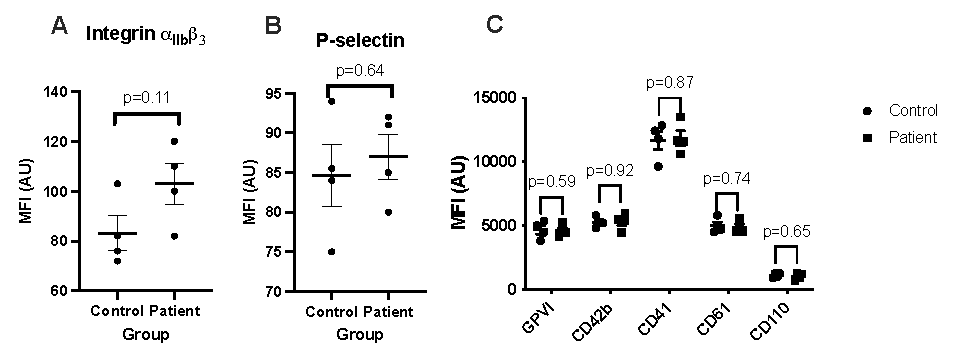
\includegraphics[width=0.9\linewidth]{figure/Bariatric_study/Basal_surface_receptors} 

}

\caption[Comparison of basal integrin α\textsubscript{IIb}β\textsubscript{3} activation, P-selectin expression and surface receptors levels across control and bariatric patient groups]{\textbf{Comparison of basal integrin α\textsubscript{IIb}β\textsubscript{3} activation, P-selectin expression and surface receptors levels across control and bariatric patient groups.} Diluted PRP was used for experiments, where platelets were incubated with antibodies for 10 minutes before fixing. Bar graphs comparing A) Basal integrin α\textsubscript{IIb}β\textsubscript{3} activation B) Basal P-selectin expression and C) Basal surface receptor expression across bariatric patient and control groups. Antibodies were used to detect surface expression of GPVI, CD42b (GP1bα), CD41 (integrin α\textsubscript{IIb}), CD61 (Integrin β\textsubscript{3}) and CD110 (thrombopoietin/TPO receptor). N=4. P-values indicated for unpaired t-test results. Mean + SEM displayed.}\label{fig:basal-integrin-pselectin-receptor-bariatric}
\end{figure}
\hypertarget{agonist-induced-integrin-ux3b1iibux3b23-activation-and-p-selectin-expression}{%
\subsection{\texorpdfstring{Agonist-induced integrin α\textsubscript{IIb}β\textsubscript{3} activation and P-selectin expression}{Agonist-induced integrin αIIbβ3 activation and P-selectin expression}}\label{agonist-induced-integrin-ux3b1iibux3b23-activation-and-p-selectin-expression}}

Markers of platelet activation were compared in response to different platelet agonists. There was weak evidence that the integrin α\textsubscript{IIb}β\textsubscript{3} maximum response was reduced in the bariatric patient group in response to PAR1-AP (2479 AU (SEM 126) in control vs 2105 AU (SEM 101) in bariatric group, p=0.06) and ADP (2526 AU (SEM 121) in control group vs 2274 AU (SEM 478), p=0.05), but there was no change in the pEC50s across groups (Figure \ref{fig:agonist-integrin-pselectin}). There was insufficient data to compare the pEC50s and max of the curves for CRP, however comparing the highest concentration of CRP, there was no difference in response across the bariatric and control group for activation of the integrin α\textsubscript{IIb}β\textsubscript{3} (Figures \ref{fig:agonist-integrin-pselectin}A-C). There was no difference in the levels of P-selectin across bariatric patients and control groups in response to PAR1-AP or ADP (Figures \ref{fig:agonist-integrin-pselectin}D and E) as determined by the pEC50 or the curve maximum values. There was no evidence for a difference in expression of P-selectin across bariatric and control groups in response to the highest concentration of CRP (Figure \ref{fig:agonist-integrin-pselectin}F).



\begin{figure}

{\centering 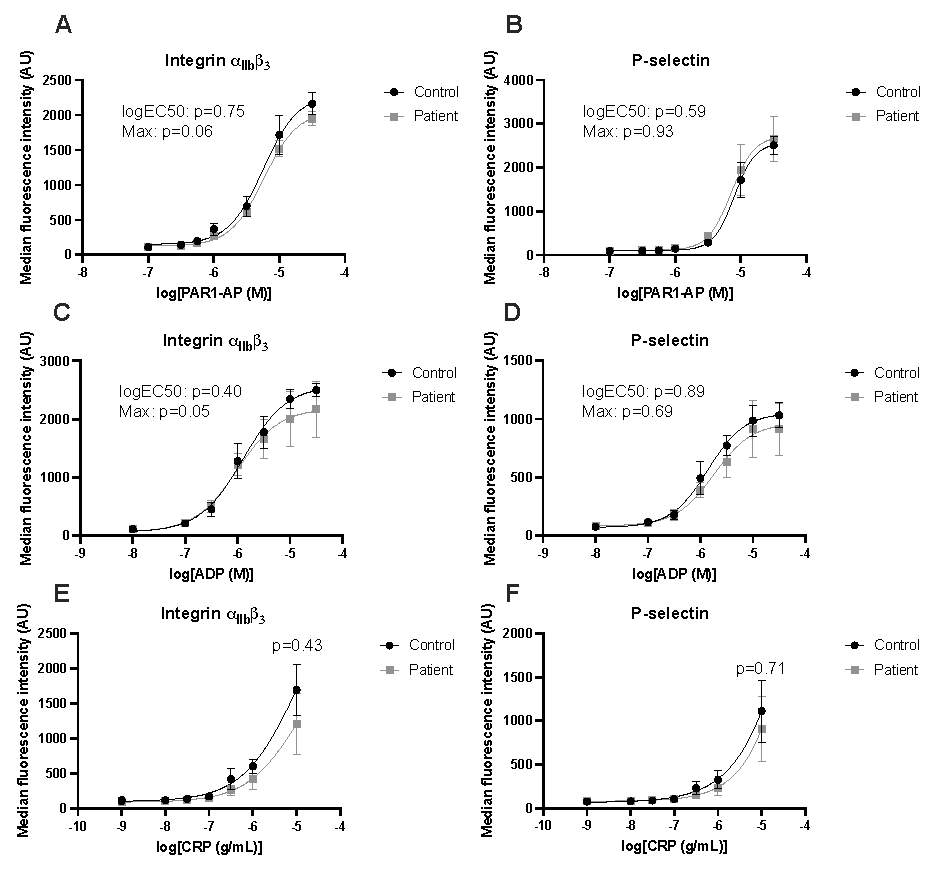
\includegraphics[width=0.9\linewidth]{figure/Bariatric_study/Agonist_Integrin_Pselectin} 

}

\caption[Concentration-response curves of integrin α\textsubscript{IIb}β\textsubscript{3} activation and P-selectin expression for bariatric patient and control groups]{\textbf{Concentration-response curves of integrin α\textsubscript{IIb}β\textsubscript{3} activation and P-selectin expression for bariatric patient and control groups} in platelet rich plasma diluted in HEPES-Tyrode's. Integrin α\textsubscript{IIb}β\textsubscript{3} activation in response to A) PAR1-AP, B) ADP and C) CRP. P-selectin expression in response to D) PAR1-AP, E) ADP, F) CRP. N=4. Mean ± SEM displayed. P values are the comparison of either the pEC50 or the maximum of the curve for the individual concentration-response curves across the bariatric patient and control groups. For CRP, the p value for an unpaired two-tailed t-test comparing the response to 1x10\textsuperscript{-5} g/mL CRP across the bariatric patient and control groups is displayed.}\label{fig:agonist-integrin-pselectin}
\end{figure}
\hypertarget{platelet-neutrophil-aggregates}{%
\subsection{Platelet-neutrophil aggregates}\label{platelet-neutrophil-aggregates}}

Platelets also are important in the inflammatory response, where they interact with other key innate immune system cells such as neutrophils. Platelets can bind to neutrophils through the P-selectin receptor. Platelet-neutrophil interactions were explored across groups to determine whether there was a difference in the proportion of neutrophils that are bound to platelets, therefore demonstrative of a difference in hyperactive platelets. This was explored by gating neutrophils using an antibody for the specific neutrophil marker, CD45, and their side scatter (granularity). Within this gate, the percentage of neutrophils interacting with platelets was determined by using an antibody for the platelet specific marker CD41 (integrin α\textsubscript{IIb} subunit) and determining the percentage of events that were both CD45+ and CD41+. There was no difference in the percentage of neutrophils bound to platelets under basal conditions (7.0 \% (SEM 1.5 \%) in control v 11.2 \% (SEM 3.2\%) in bariatric patient group, p=0.30). Similarly, after stimulation with CRP, there was no difference in the percentage of neutrophil-platelet aggregates (38.6 \% (SEM 2.6 \%) in control group v 35.5 \% (SEM 2.7 \%), p=0.48).



\begin{figure}

{\centering 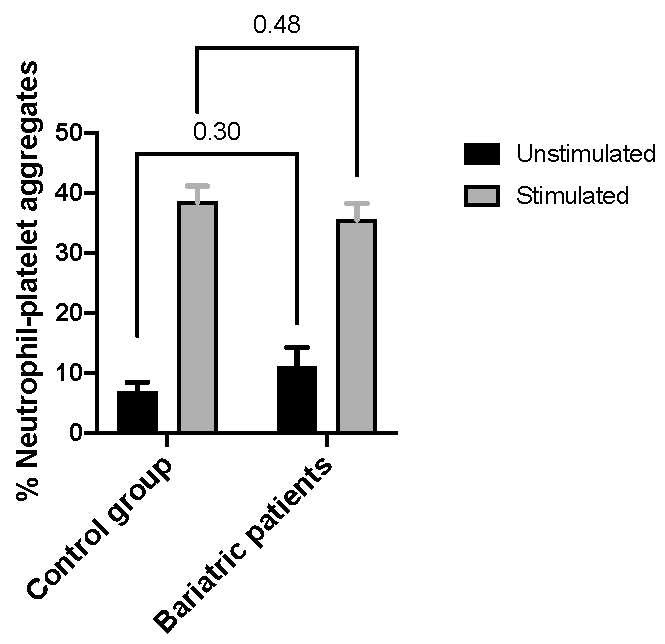
\includegraphics[width=0.7\linewidth]{figure/Bariatric_study/Plt-neu_aggregates} 

}

\caption[Comparison of neutrophil-platelet aggregates across bariatric and control groups.]{\textbf{Comparison of neutrophil-platelet aggregates across bariatric and control groups.} Neutrophil-platelet aggregates were determined using CD45 and CD41 antibodies. Aggregates were compared across bariatric patient and control participant groups in unstimulated and stimulated (5 ug/mL CRP) conditions. N=4. P-values provided for the results of a two-way ANOVA with Sidak's multiple comparisons tests. Mean + SEM displayed.}\label{fig:platelet-neutrophil}
\end{figure}
\hypertarget{platelet-proteomics}{%
\subsection{Platelet proteomics}\label{platelet-proteomics}}

The platelet proteome holds important information about platelet signalling. Differential expression of proteins across bariatric patients and controls was therefore explored. A total of 5318 proteins were detected from platelets of both groups of participants by tandem mass tag mass spectrometry (TMT-MS). A principal component analysis (PCA) was performed on the protein data. PC1 and PC2 explained 27.1 \% and 14.4 \% of the variance in the data, respectively. A PC plot of PC1 against PC2 is shown in Figure \ref{fig:pca}. PC1 plotted against PC2 did not separate the bariatric patient samples from the control participant samples, despite grouping of three patients (Figure \ref{fig:pca}). PC3 and PC4 explained 13.1\% and 12.6\% of the data respectively. When plotting PC3 against PC4, there is separation among the groups (Figure \ref{fig:pca2}). This suggests that the group was not the main source of variation between the data.



\begin{figure}

{\centering 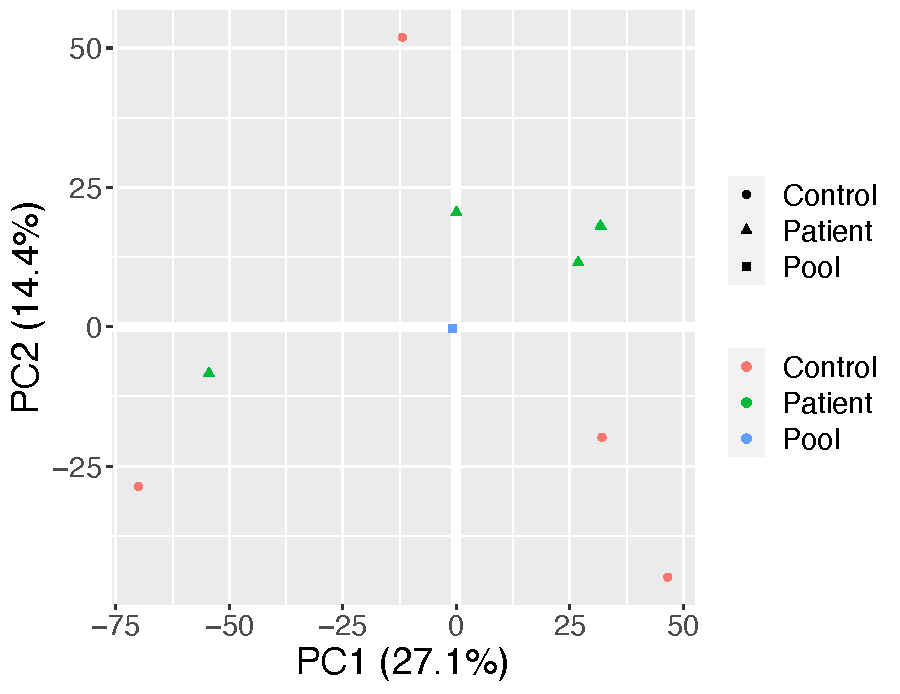
\includegraphics[width=0.8\linewidth]{figure/Bariatric_study/Proteomic_PCA} 

}

\caption[Principal component analysis (PCA): scatter plot of PC1 and PC2]{\textbf{Principal component analysis (PCA): scatter plot of PC1 and PC2.} Each point represents a participant. Control samples are coloured red and bariatric samples coloured blue, with the pooled reference sample of both control and bariatric samples coloured in blue.}\label{fig:pca}
\end{figure}


\begin{figure}

{\centering \includegraphics[width=0.8\linewidth]{figure/Bariatric_study/PC3vPC4_proteomics} 

}

\caption[Principal component analysis (PCA): scatter plot of PC3 and PC4.]{\textbf{Principal component analysis (PCA): scatter plot of PC3 and PC4.} Each point represents a participant. Control samples are coloured pink and bariatric samples coloured blue, with the pooled reference sample of both control and bariatric samples coloured in blue.}\label{fig:pca2}
\end{figure}
There was evidence (p\textless0.05) that 188 out of a total of 5318 detected platelet proteins (3.5\%) were altered in bariatric patients with obesity compared to controls (Figure \ref{fig:volcano}). Positive logFC values indicate the protein having higher levels in the bariatric group. The protein which had the strongest evidence for a BMI effect was phosphatidylinositol 4-kinase beta (PI4K-beta) (logFC 0.45, p=6.3x10\textsuperscript{-5}). The signalling protein G protein-coupled receptor kinase (GRK6) was lower in bariatric patients (logFC -0.15, p=0.002), whereas the adipocyte plasma membrane-associated protein (APMAP) was increased in bariatric patients (logFC 0.23, p=0.006). Platelet proteins previously reported\textsuperscript{\protect\hyperlink{ref-Barrachina2019}{99}} to be associated with BMI replicated here, including gelsolin (logFC -0.14, p=0.018), actin (cytoplasmic 1, logFC 0.51, p=0.03) and septin-2 (logFC 0.14, p=0.03). Platelet transcripts have been reported to be associated with BMI, including transcripts for myeloperoxidase and protein S100-A9\textsuperscript{\protect\hyperlink{ref-Freedman2010}{125}}. The current study provides evidence that these alterations in transcripts directly relate to protein levels measured in the proteomics analysis as BMI group was associated with both myeloperoxidase (LogFC 1.15, p=0.04) and protein S100-A9 (logFC 1.48, p=0.049). Similar to the flow cytometry results, no alteration in protein receptors such as the α\textsubscript{IIb} integrin and GPVI receptor was detected. The full platelet proteomic results can be found here \url{https://github.com/lucygoudswaard/mythesis/blob/f17f0250ad50bad74d7e38225d060aa6cd83321b/index/figure/Bariatric_study/Proteomics_results.xlsx}



\begin{figure}

{\centering \includegraphics[width=0.8\linewidth]{figure/Bariatric_study/volcano_proteomics_labelled} 

}

\caption[A volcano plot comparing the Log\textsubscript{2} fold change in protein levels in bariatric patients compared to controls]{\textbf{A volcano plot comparing the Log\textsubscript{2} fold change in protein levels in bariatric patients compared to controls.} Dashed lines indicate a log\textsubscript{2} fold change of 0.3 and a pvalue cut off of 0.05 (-Log\textsubscript{10} pvalue of 1.3)}\label{fig:volcano}
\end{figure}
\hypertarget{discussion-1}{%
\section{Discussion}\label{discussion-1}}

This chapter explored the effect of obesity on platelet parameters and platelet function by collecting pre-surgery samples from bariatric patients and age and sex-matched controls. Here, I have optimised common experimental laboratory techniques for use within a patient study. In addition, these techniques have also been used to study platelet function within another patient group (COVID-19) and can be implemented in future patient studies. The present study did not detect functional differences in platelet parameters and between bariatric patients compared to healthy controls, but proteomics analysis by TMT-MS detected differences in platelet protein abundance, which may have implications for platelet signalling.

This study did not detect differences in platelet characteristics such as IPC when comparing the high BMI bariatric surgery group with the control group. The small sample size and large standard deviation in the high BMI group would explain why the BMI and IPC association detected in Chapter \ref{BMI-platelets-INTERVAL} was not detected in the current study. There was also no evidence for a difference in levels of platelet receptors under basal conditions. A difference in P-selectin expression in response to agonists across the bariatric patient and control group was not detected, however, there was weak evidence that activation of the integrin α\textsubscript{IIb}β\textsubscript{3} was impaired in the bariatric patient group. This reduction is modest so it is unclear whether this would impact the ability of platelets to aggregate. A previous study (unpublished) from the Hers group and published data from other groups\textsuperscript{\protect\hyperlink{ref-Taus2020}{126}} indicated that in severe COVID-19 there is a large reduction (\textasciitilde60\% reduction) in platelet integrin α\textsubscript{IIb}β\textsubscript{3} activation, but an increase in the percentage of platelets bound to neutrophils therefore suggesting there is hyperactivity. It is therefore possible that impaired integrin activation may be a marker of platelet hyperactivity. A similar reduction in integrin α\textsubscript{IIb}β\textsubscript{3} activation was reported in platelets from patients with myeloproliferative disorders who also have a prothrombotic phenotype\textsuperscript{\protect\hyperlink{ref-Moore2013}{127}}. In the current study there a small reduction in integrin α\textsubscript{IIb}β\textsubscript{3} activation (\textasciitilde10\% reduction in the bariatric surgery group in response to ADP). Replication in a larger sample size is important to further characterise differences integrin α\textsubscript{IIb}β\textsubscript{3} activation.

One previous study detected an increase in GPVI receptor levels and GPVI mediated platelet aggregation\textsuperscript{\protect\hyperlink{ref-Barrachina2019}{99}}. Despite this previous finding, Barrachina et al.~did not directly measure activation of the integrin α\textsubscript{IIb}β\textsubscript{3}, so it is unclear how this increase in expression would translate to the activation of this integrin. A larger sample size would be required to be able to draw conclusions here. As well as this, aggregation experiments would have also been useful to compare platelet function across groups, however this technique was not chosen due to time restraints and large amount of sample required.

The principal component analysis of the proteomic data suggested that PC4 was able to separate the bariatric and control groups. Although PC4 was not the main source of variance, even with a small N number, this provided evidence that the group (bariatric/control) could explain variation in proteins. Therefore, some protein signatures may be due to the difference in BMI. However, it could also be due to other factors which differed across groups such as previous COVID-19 infection or T2D diagnosis. COVID-19 infection can cause venous thromboembolism and is more likely to occur in people with obesity\textsuperscript{\protect\hyperlink{ref-Klok2020}{114},\protect\hyperlink{ref-McFadyen2020}{128},\protect\hyperlink{ref-Wang2021}{129}}. Therefore, it is possible that the COVID-19 infection in the bariatric patients may cause longer-term changes in platelet activity and confound results. Despite this, concordance with previous studies in terms of proteins reportedly altered with BMI also suggests that the current study is likely capturing platelet protein signatures of obesity. Table \ref{tab:proteome-lit} shows the results that have replicated in the current study when comparing to three previous studies that have studied the platelet proteome\textsuperscript{\protect\hyperlink{ref-Barrachina2019}{99}}, platelet microvesicle proteome\textsuperscript{\protect\hyperlink{ref-Grande2019}{130}} and platelet transcriptome in relation to obesity\textsuperscript{\protect\hyperlink{ref-Freedman2010}{125}}.



\begin{landscape}\begin{table}

\caption[Summary of current literature on the effect of body mass index on the platelet proteome]{\label{tab:proteome-lit}\textbf{Summary of current literature on the effect of body mass index on the platelet proteome}}
\centering
\begin{tabu} to \linewidth {>{\raggedright\arraybackslash}p{5cm}>{\raggedright\arraybackslash}p{3cm}>{\raggedright\arraybackslash}p{9cm}}
\toprule
Paper & Author, year & Overlapping findings\\
\midrule
GPVI surface expression and signalling pathway activation are increased in platelets from obese patients: Elucidating potential anti-atherothrombotic targets in obesity & Barrachina et al., 2019 & Proteins altered: Actin, cytoplasmic 1 (Fragment), Septin-2, Gelsolin, Glycerol-3-phosphate dehydrogenase\\
Platelet-Derived Microparticles From Obese Individuals: Characterization of Number, Size, Proteomics, and Crosstalk With Cancer and Endothelial Cells & Grande et al., 2019 & Platelet microvesicle proteins altered: LIM and senescent cell antigen-like containing domain protein 1\\
Relation of platelet and leukocyte inflammatory transcripts to body mass index in the Framingham heart study & Freedman et al., 2010 & Platelet transcripts altered: myeloperoxidase (MPO), S100-A9\\
\bottomrule
\end{tabu}
\end{table}
\end{landscape}
Evidence from the current study and results from Barrachina et al\textsuperscript{\protect\hyperlink{ref-Barrachina2019}{99}}. point towards platelet proteins which may be altered with obesity such as actin, gelsolin and septin-2. Actin is important in platelet shape change and activation\textsuperscript{\protect\hyperlink{ref-Barrachina2019}{99},\protect\hyperlink{ref-Bearer2002}{131}}. Higher actin levels in platelets from patients with obesity could contribute to platelet hyperactivity. Mutations in the gene which encodes actin (ACTB) can cause Baraitser-Winter cerebrofrontofacial syndrome (BWCFF). Patients with this syndrome have been reported to have a low platelet count (thrombocytopenia) with enlarged platelets and a higher immature platelet fraction\textsuperscript{\protect\hyperlink{ref-Latham2018}{132}}. This actinopathy is known as ACTB-associated syndromic thrombocytopenia. It is therefore possible that increased levels of actin may be indicative of more newly produced platelets. Gelsolin is another platelet cytoskeletal protein, which was lower in the bariatric patient group. Gelsolin levels were shown to be lower in PRP from patients with stable angina pectoralis compared with controls, however they were higher in patients with unstable angina pectoralis and acute myocardial infarction patients\textsuperscript{\protect\hyperlink{ref-Yue2011}{133}}. Recombinant human gelsolin has been shown to be protective against thromboembolism in mice, thereby suggesting that reduced levels seen in the current study could increase thrombosis risk\textsuperscript{\protect\hyperlink{ref-Gupta2019}{134}}. Septins are cytosolic proteins which are also reported to be important in integrin α\textsubscript{IIb}β\textsubscript{3} activation, platelet spreading and clot contraction\textsuperscript{\protect\hyperlink{ref-Kim2020}{135}}. Septin-2 levels were higher in platelets from bariatric patients, suggesting this may lead to increased platelet activation. Although no difference was found in α\textsubscript{IIb}β\textsubscript{3} activation, it would be useful to explore whether there are differences in platelet aggregation and platelet spreading.

There is also overlap between platelet proteins altered with BMI in the current study and platelet transcripts that are reported to be altered with higher BMI\textsuperscript{\protect\hyperlink{ref-Freedman2010}{125}}. For example, S100A9 (Myeloid-related protein-14 or MRP-14) transcripts were altered with BMI and the levels of the protein were increased in the bariatric group in the current study. Studies in mice have found evidence that S100A9 is involved in thrombus formation\textsuperscript{\protect\hyperlink{ref-Wang2014a}{136}}, and there is evidence for its involvement in myocardial infarction\textsuperscript{\protect\hyperlink{ref-Cai2020}{137}}. Likewise, myeloperoxidase (MPO) transcripts were associated with BMI and there were higher protein levels in bariatric patients with obesity. A previous study has shown evidence that MPO can potentiate ADP-induced platelet aggregation in PRP\textsuperscript{\protect\hyperlink{ref-Gorudko2013}{138}}.

These platelet proteins have previously been reported to be associated with BMI and are therefore more likely to be robust associations. This study has also provided some novel platelet proteins which have different levels in bariatric patients with obesity compared with healthy weight controls. For example, there was an increase in levels of APMAP in platelets from the high BMI group. A SNP which is associated with higher plasma levels of APMAP (rs8125909) is associated with higher BMI and greater weight\textsuperscript{\protect\hyperlink{ref-Liu2021}{139}}, therefore it is possible that the protein is involved in weight regulation, rather than higher BMI altering levels of the protein. Following up this protein after bariatric surgery could help determine the directionality of the effect. There was also a decrease in levels of G protein-coupled receptor kinase (GRK6) in the high BMI group. GRKs phosphorylate G protein coupled receptors (GPCRs) that have been activated by agonists, thereby leading to receptor desensitisation\textsuperscript{\protect\hyperlink{ref-Chaudhary2020}{140}}. GRK6 knockout mice have been shown to have larger aggregatory responses to agonists and more dense and α-granule secretion, along with increased thrombus formation\textsuperscript{\protect\hyperlink{ref-Chaudhary2020}{140}} as a result of less receptor desensitisation occurring. Together, these results therefore reflect a platelet proteomic footprint of higher BMI that implicates a hyperactive platelet environment. Investigating the role of these proteins would be informative. It would also be important to explore additional measures of platelet activation such as platelet aggregation, calcium mobilisation and in vitro thrombus formation, as well as replicating experiments in a larger cohort.

In the proteomics analysis, a post hoc power calculation was performed to determine the range of power for the effect sizes where p\textless0.05. This study had at least 67\% power to detect effect sizes, but for some proteins which had smaller p values, there was 100\% power. A larger sample size would be required to be able to detect smaller effect sizes.

Overall, this study optimised experimental techniques to test platelet function from patients. Sample sizes were limited and only small differences were detected in platelet function experiments and Sysmex platelet parameters. Platelet proteomic analysis replicated previous findings in relation to proteins which may be altered by BMI and implicated some novel proteins which are altered by BMI and may lead to changes in platelet function. Larger sample sizes of participants which display more similar characteristics would be required to confirm findings.

\hypertarget{chemokine-platelets}{%
\chapter{Pathways linking plasma proteins and platelet function: do the chemokines MDC and TARC play a role?}\label{chemokine-platelets}}

\hypertarget{background-3}{%
\section{Background}\label{background-3}}

Platelets play an important role in haemostasis\textsuperscript{\protect\hyperlink{ref-Rivera2009}{35}}. In healthy people, prostacyclin (PGI2) and nitric oxide (NO) are released by the endothelium to suppress platelet activity\textsuperscript{\protect\hyperlink{ref-Yau2015}{36}}. When the endothelium is damaged, platelets adhere to the injured vessel wall through the glycoprotein Ib-IX-V receptor and the GPVI collagen receptor. As a result, platelets secrete α- and dense-granules and undergo shape change\textsuperscript{\protect\hyperlink{ref-Badimon2012}{23}}. Alpha granules release growth factors (e.g.~IGF-1), clotting factors and chemokines\textsuperscript{\protect\hyperlink{ref-Gear2003}{37}}, whereas dense granules release molecules such as ADP, which further activate platelets by interacting with the P2Y\textsubscript{1} and P2Y\textsubscript{12} platelet receptors. Platelet activation also results in activation of integrins such as α\textsubscript{IIb}β\textsubscript{3} and subsequent fibrinogen binding results in platelet aggregation, thrombus formation and cessation of bleeding\textsuperscript{\protect\hyperlink{ref-Rivera2009}{35}}. Despite these processes being essential for haemostasis, when platelets become hyperactive, the balance is tipped in favour of thrombosis.

Platelets likely contribute to the increased CVD risk related to obesity and type II diabetes. Platelets from patients with obesity are reported to be hyperactive and have a lower sensitivity to antiplatelet therapies such as clopidogrel\textsuperscript{\protect\hyperlink{ref-Nardin2015}{44}}. These therapies are critical in the prevention of ischaemic events in certain circumstances. The underlying mechanism that causes platelet hyperactivity is not completely understood. It is likely to involve a combination of factors. One such factor is a decrease in the production of endothelial PGI2 and nitrous oxide\textsuperscript{\protect\hyperlink{ref-BelindeChantemele2012a}{141}}. Another contributing factor could be an alteration in the circulating levels of soluble ligands, growth factors and cytokines as a result of low grade chronic inflammation\textsuperscript{\protect\hyperlink{ref-Esser2014}{86}}. These proteins may subsequently enhance platelet function (known as platelet priming). Platelet primers are signaling molecules which enhance agonist-induced platelet function but in isolation are unable to activate platelets. Molecules that have been reported to be able to prime platelets include insulin-like growth factor-1 (IGF-1)\textsuperscript{\protect\hyperlink{ref-Nardin2015}{44},\protect\hyperlink{ref-Blair2015}{76}} and thrombopoietin (TPO)\textsuperscript{\protect\hyperlink{ref-Maury2010a}{73}}.

There are other biomarkers which are also suggested to be raised with obesity as a result of low-grade chronic inflammation\textsuperscript{\protect\hyperlink{ref-Esser2014}{86}}, including the chemokines macrophage-derived chemokine (MDC/CCL22) and thymus and activation regulated chemokine (TARC/CCL17)\textsuperscript{\protect\hyperlink{ref-Safa2016}{142}}. These inflammatory chemokines act at the receptor CCR4, which is expressed on platelets\textsuperscript{\protect\hyperlink{ref-Clemetson2000}{143}}. MDC and TARC have been shown to potentiate platelet aggregation\textsuperscript{\protect\hyperlink{ref-Gear2001}{144}}. For example, the presence of TARC and MDC have been demonstrated to greatly enhance platelet aggregation in the presence of low levels of the platelet agonist ADP\textsuperscript{\protect\hyperlink{ref-Gear2001}{144}}. Furthermore, gene polymorphisms of MDC and CCR4 are associated with myocardial infarction (MI), therefore implicating MDC in thrombosis pathophysiology\textsuperscript{\protect\hyperlink{ref-Noori2018}{91}}. Previous studies have shown that multiple platelet primers increase platelet function through activation of the lipid kinase phosphoinositide-3-kinase (PI3K)\textsuperscript{\protect\hyperlink{ref-Blair2015}{76},\protect\hyperlink{ref-Pasquet2000}{77},\protect\hyperlink{ref-Falcinelli2005}{145}}. Another pathway that has been implicated in platelet priming effects is the mitogen-activated protein kinase (MAPK) pathway. TPO can enhance thromboxane A\textsubscript{2} (TxA\textsubscript{2}) synthesis through increasing the activation of extracellular signal regulated kinase (ERK2)\textsuperscript{\protect\hyperlink{ref-Ezumi1998}{82},\protect\hyperlink{ref-VanWilligen2000}{83}}. The common involvement of both PI3K and MAPK pathways in platelet priming mediated by IGF-1, TPO and matrix metalloproteinase-2 (MMP-2) suggests that MDC and TARC could also exert priming effects through these common pathways.

As blood/plasma levels of MDC have been reported to be elevated in obese people\textsuperscript{\protect\hyperlink{ref-Safa2016}{142}} and polymorphisms of its receptor are associated with MI, understanding the mechanisms by which MDC can enhance platelet function may provide important insight in to how platelets are hyperactive in obesity and potentially provide a novel target for new antiplatelet/thrombotic or preventative therapies for those with an increased risk of cardiovascular events.

The aims of this chapter are therefore to:
\begin{enumerate}
\def\labelenumi{\arabic{enumi})}
\tightlist
\item
  Determine the effects and mechanisms of MDC and TARC on platelet function and signalling.
\item
  Explore the effect of increasing levels of MDC and TARC on disease using two sample Mendelian randomization.
\end{enumerate}
Figure \ref{fig:chemokine-platelet-graphic} indicates the parts of the overal thesis hypthoses which are addressed in the current chapter.



\begin{figure}

{\centering \includegraphics[width=0.9\linewidth]{figure/Chemokines/Thesis_graphic_overview_chemokines} 

}

\caption[Schematic of the associations explored in Chapter \ref{chemokine-platelets}]{\textbf{Schematic of the associations explored in Chapter \ref{chemokine-platelets}}. This chapter explores the effect of the chemokines MDC and TARC on platelet function and aims to explore their involvement in disease. Figure made using BioRender.com.}\label{fig:chemokine-platelet-graphic}
\end{figure}
\hypertarget{methods-1}{%
\section{Methods}\label{methods-1}}

\hypertarget{materials-1}{%
\subsection{Materials}\label{materials-1}}

Materials used for the current chapter are listed in section \ref{materials}.

\hypertarget{isolation-of-human-platelets}{%
\subsection{Isolation of human platelets}\label{isolation-of-human-platelets}}

Fresh human venous blood was obtained from healthy volunteers by venipuncture. Blood was taken into the syringe with a 1 in 10 volume of 4 \% trisodium citrate, then mixed with a 1 in 7 volume of acid citrate dextrose (ACD). Blood was placed into 5 mL LP4 tubes then centrifuged at 1000 revolutions per minute (RPM) for 17 minutes. Platelet rich plasma (PRP) was removed. PRP was supplemented with inhibitors such as 0.02 U/mL apyrase, 140 nM PGE1 or 10 µM indomethacin. Supplemented PRP was either used for the experiment or centrifuged for a further 10 minutes at 1700 RPM. Platelet poor plasma (PPP) was removed leaving a platelet pellet. This pellet was resuspended in HEPES Tyrode's (supplemented with 0.1 \% glucose and 0.02 U/mL apyrase, and 10 µM indomethacin if already applied to PRP). Platelets were counted using a Z1 coulter particle counter by diluting 1 in 2000 in 10 mL MQ water. Platelets were diluted further using the supplemented HEPES Tyrode's to a platelet concentration of 4 x 10\textsuperscript{8}/mL and left to rest for 30 mins in a 30°C water bath.

\hypertarget{integrin-ux3b1iibux3b23-activation-and-p-selectin-expression-measured-by-flow-cytometry-1}{%
\subsection{\texorpdfstring{Integrin α\textsubscript{IIb}β\textsubscript{3} activation and P-selectin expression measured by flow cytometry}{Integrin αIIbβ3 activation and P-selectin expression measured by flow cytometry}}\label{integrin-ux3b1iibux3b23-activation-and-p-selectin-expression-measured-by-flow-cytometry-1}}

Washed platelets were diluted to a concentration of 2 x 10\textsuperscript{7}/mL using supplemented HEPES Tyrode's buffer with FITC-conjugated PAC1 and PE-conjugated CD62P antibodies in a 2:1 ratio, where PAC1 was present at a 1:10 volume and CD62P at 1:20. Platelets were incubated with 200 ng/ml MDC, TARC or vehicle for 5 mins followed by stimulation with increasing concentrations of PAR1-AP for 10 minutes. Platelets were fixed with a final concentration of 1 \% paraformaldehyde (PFA) for 10 minutes. Plates were analysed using the BD Accuri C6 Plus flow cytometer (BD Biosciences, Wokingham, UK), where the median fluorescence intensity was derived from 10,000 gated platelets.

\hypertarget{platelet-aggregation}{%
\subsection{Platelet aggregation}\label{platelet-aggregation}}

Platelets were diluted to a concentration of 2 x 10\textsuperscript{8}/mL using supplemented HEPES Tyrode's buffer. A volume of 250 µL platelets was added to aggregometer cuvettes containing a Teflon stir bar. HEPES Tyrode's (500 µL) was added to the reference PPP (blank) channel. Platelets were left to rest in the cuvettes for 2 mins. For priming experiments, platelets were either preincubated with vehicle (MQ) or 1 µg/ml MDC or TARC for 5 mins. A Chrono-log model 490 aggregometer was used. For experiments which were not exploring platelet priming, platelets were added to the cuvettes for 2 minutes and agonist was added for 5 minutes. Aggregation traces were derived from the amount of light transmitted through the sample. Recordings were taken for 5 minutes with a stirring speed of 1200 RPM and at 37 °C. Platelets were used within 3 hours from resting.

\hypertarget{plate-platelet-aggregation}{%
\subsection{Plate platelet aggregation}\label{plate-platelet-aggregation}}

PRP supplemented with apyrase was used. For each donor, the platelet count was recorded. PPP was used as a reference. PRP was added to the wells of a 96 well plate and left to rest for 2 minutes. 200 ng/ml MDC, 200 ng/mL TARC or vehicle were preincubated with platelets for 5 minutes. After 5 minutes, PAR1-AP was added to the wells and the plate was shaken with an Eppendorf ThermoMixer® for 5 minutes at 1200 RPM and at 37 °C. The plate was immediately read using a Labtech LT-4500 automatic microplate absorbance reader. Responses were normalized so that basal PRP = 0 \% aggregation and PPP = 100 \% aggregation.

\hypertarget{phosphatidylserine-ps-exposure}{%
\subsection{Phosphatidylserine (PS) exposure}\label{phosphatidylserine-ps-exposure}}

Washed platelets were used at a concentration of 2 x 10\textsuperscript{7}/mL. Platelets were preincubated with vehicle, 200 ng/mL MDC or 200 ng/mL TARC for 5 mins. Platelets were then stimulated 5 ug/mL CRP as well as increasing concentrations of thrombin for 10 mins. PE-conjugated annexin V (1:10 v/v) was used to bind to PS. Plates were read using the BD Accuri flow cytometer, where the \% positive (annexin V) were recorded.

\hypertarget{flow-cytometry-phospho-vasp}{%
\subsection{Flow cytometry: phospho-VASP}\label{flow-cytometry-phospho-vasp}}

Washed platelets were diluted to a concentration of 1 x 10\textsuperscript{8}/mL. Platelets were left to rest in a 96 well plate for 2 minutes to warm to 37 °C. 200 ng/ml MDC, 200 ng/mL TARC, 10 µM ADP or vehicle were preincubated with platelets for 5 mins at 37 °C. PGE1 (concentration-response curve) was added for a further 5 minutes. Platelets were fixed with 1 \% PFA for 10 minutes. Platelets were centrifuged in a 96 well plate at 2651 rpm for 10 minutes (Heraeus Megafuge with M-20 Microplate Swinging Bucket Rotor, ThermoFisher Scientific). Supernatant was then discarded, and platelets were permeabilized with 0.1\% TritonTM X-100 for 10 minutes. The plate was centrifuged again at 2651 rpm for 10 minutes. Supernatant was discarded and platelets were washed and resuspended in 1 x PBS. Platelets were centrifuged at 2651 rpm for 10 minutes. Supernatant was discarded and platelets were resuspended with rabbit pSer157 VASP primary antibody (1 in 1000) for 30 minutes on ice. Platelets were centrifuged at 2651 rpm for 10 minutes. Supernatant was discarded and platelets were washed and resuspended with 1 x PBS. Platelets were centrifuged at 2651 rpm for 10 minutes. Supernatant was discarded and platelets were resuspended with secondary antibody (Alexa Fluor™ 647 anti-rabbit IgG, 1 in 1000) for 45 minutes on ice. Platelets were centrifuged at 2651 RPM for 10 minutes. Supernatant was discarded and platelets were washed with 1 x PBS. Platelets were centrifuged once more at 2651 rpm for 10 minutes, resuspended once more in 1 x PBS and the plate was read using a BD Accuri C6 Plus flow cytometer and using the APC-A channel.

\hypertarget{western-blotting}{%
\subsection{Western blotting}\label{western-blotting}}

Platelets were used at a concentration of 4 x 10\textsuperscript{8}/mL. Platelets were preincubated with 200ng/mL MDC, 200ng/mL TARC or vehicle for 5 minutes followed by 5 minutes application of PAR1-AP (all at 30 °C). For phospho-VASP assay, MDC, TARC or ADP were preincubated with platelets for 5 minutes, with PGE1 added for a further 5 minutes. Platelets were lysed with 4 X LDS NuPAGE sample buffer supplemented with 50 mM dithiothreitol (DTT). Samples were stored at -20 °C. Samples were heated to 70 °C for 10 minutes prior to SDS-PAGE. A 10 \% Resolving gel was cast for Tris-glycine SDS-polyacrylamide gel electrophoresis, and a 5 \% Stacking gel was cast for loading. As a standard, 4 µl Precision Plus protein pre-stained standard was loaded, along with 20 µl of the lysate sample. The samples were placed in a tank containing 4-morpholinepropanesulfonic acid (MOPS) running buffer (50 mm MOPS, 50 mm Tris, 1 mm EDTA, 0.1\% SDS, 5 mm sodium bisulfite) and protein electrophoresis was carried out for 90 minutes at 100 V. Following this, proteins were transferred to a poly(vinylidene fluoride) (PDVF) membrane in the presence of transfer buffer (25 mM Tris-HCl (pH 7.6), 192 mM glycine, 20\% methanol) for 60 minutes and at 100 V. The membrane was then incubated in LI-COR blocking buffer with 0.1 \% TBS-Tween in a 1:1 ratio for 1 hour. Membranes were incubated with the primary antibody (1 in 1000 dilution) at room temperature overnight. Talin was used as a loading control. The membrane was washed 3 times with 0.1 \% TBS-Tween for 5 minutes. The membrane was incubated with Fluor680 labelled secondary antibody (1 in 5000 dilution) for 1 hour. The membrane was washed 6 times for 5 minutes, then membranes were scanned using the LI-COR Odyssey® CLx Imaging System. Bands were quantified using Image Studio Lite.

\hypertarget{calcium-mobilisation}{%
\subsection{Calcium mobilisation}\label{calcium-mobilisation}}

Fura-2 (4 µM) was added to PRP after the addition of indomethacin and apyrase and incubated for 1 hour wrapped in foil at 37 °C. PRP was centrifuged and platelets were resuspended in supplemented HEPES Tyrode's as described above, with washed platelets (at 4 x 10\textsuperscript{8}/mL) protected from the light with foil. Platelets were recalcified with 1 mM calcium chloride using the Tecan Infinite M200 multimode plate reader (Mannedorf, Switzerland). Fluorescence of fura-2 was measured as the ratio at wavelengths 340:380 nm and provided a measurement of free calcium. 10 basal recordings were taken over 1 minute before addition of MDC, TARC or ADP. Upon agonist stimulation, 20 readings were taken over 2 minutes. A final concentration of 1 \% Triton X-100 was added to permeabilise platelets and further readings were raken as a reference for maximum calcium mobilisation.

\hypertarget{statistical-analysis-for-platelet-function-assays-1}{%
\subsection{Statistical analysis for platelet function assays}\label{statistical-analysis-for-platelet-function-assays-1}}

Data was analysed using GraphPad Prism 8. If data displayed a normal distribution (based on Shapiro-Wilk p-value and W statistic), a parametric test was used (e.g.~unpaired t-test or one way ANOVA), otherwise a nonparametric test was used. Concentration-response curves were plotted using a four parameter variable slope. To compare concentration-response curve parameters, pEC50s or curve maxes were compared. A Fisher's exact test was used to compare proportions of categorical variables. Statistical tests used for each experiment are in figure legends. Strength of evidence is determined by p-values, however results will not be dichotomised as either `significant' or `not significant'\textsuperscript{\protect\hyperlink{ref-Sterne2001}{123}}.

\hypertarget{two-sample-mr-look-up-using-epigrahdb}{%
\subsection{Two sample MR look-up using EpigrahDB}\label{two-sample-mr-look-up-using-epigrahdb}}

Mendelian randomization is a method which uses genetic variants as instrumental variables to provide a causal estimate of the relationship between a modifiable exposure and health outcome\textsuperscript{\protect\hyperlink{ref-Davies2018}{12}}. Two sample MR uses summary statistics and allows for causal effects to be estimated where the exposure and outcome are measured in different populations\textsuperscript{\protect\hyperlink{ref-Davies2018}{12}}. EpigraphDB is a tool which performs two sample MR to determine how the human proteome contributes to complex diseases\textsuperscript{\protect\hyperlink{ref-Zheng2020}{146}}. Protein quantitative trait loci (pQTLs) were available for MDC and TARC from the INTERVAL study (N=3301), which were rank normal transformed\textsuperscript{\protect\hyperlink{ref-Sun2018}{34}}. Therefore a systematic exploration of the possible roles of MDC and TARC in disease was performed. These SNPs were associated with these proteins at p\textless5x10\textsuperscript{-8}. GWAS summary statistics that were publically available for disease outcomes were included. A list of the available outcomes are presented on EpigraphDB \url{https://www.epigraphdb.org/pqtl/list/outcomes}. As an example, the venous thromboembolism variables were from Neale lab: \url{https://github.com/Nealelab/UK_Biobank_GWAS}). The venous thromboembolism (VTE) units are derived from a case/control linear mixed model. For MDC, there was one instrument available, therefore a Wald ratio was used to estimate the causal effect\textsuperscript{\protect\hyperlink{ref-Lawlor2008}{147}}. There were two instruments available for TARC, therefore the inverse variance weighted (IVW) method was used, which assumes all genetic variants are valid instrumental variables\textsuperscript{\protect\hyperlink{ref-Burgess2013}{148}}. The pQTLs used were trans pQTLs(located \textgreater500 kb from the leading pQTL). The instruments used were categorised as Tier 1 instruments, which passed both pleiotropy and consistency tests\textsuperscript{\protect\hyperlink{ref-Zheng2020}{146}}. As a total of 225 outcomes were searched, a Bonferroni-adjusted p-value of 0.05/225 = 2.2x10\textsuperscript{-4} was utilised to account for multiple testing.

\hypertarget{results-2}{%
\section{Results}\label{results-2}}

\hypertarget{priming-effects-of-mdc-and-tarc-on-platelet-aggregation-in-washed-platelets-using-light-transmission-aggregometry}{%
\subsection{Priming effects of MDC and TARC on platelet aggregation in washed platelets using light transmission aggregometry}\label{priming-effects-of-mdc-and-tarc-on-platelet-aggregation-in-washed-platelets-using-light-transmission-aggregometry}}

To investigate the effect of MDC and TARC on agonist-induced platelet aggregation, MDC and TARC were preincubated before addition of PAR1-AP. Figure \ref{fig:MDC-TARC-agg}A shows an example aggregation trace from one donor where PAR1-AP and vehicle induced only shape change, but the presence of MDC and TARC induced a maximal aggregation response. A submaximal concentration of PAR1-AP (ranging from 0.7 to 1 µM) and vehicle induced a mean aggregation of 7.0 \% (SEM 2.9 \%) aggregation (Figure \ref{fig:MDC-TARC-agg}B). In the presence of 1 µg/ml MDC, this aggregation increased to 33 \% (SEM 13 \%) (MDC v vehicle, p = 0.15). In the presence of 1 µg/ml TARC, there was 46 \% (SEM 11 \%) aggregation (TARC v vehicle, p \textless{} 0.05). Similar effects were observed with MDC and TARC on the area under the aggregation curve (Figure \ref{fig:MDC-TARC-agg}C).



\begin{figure}

{\centering 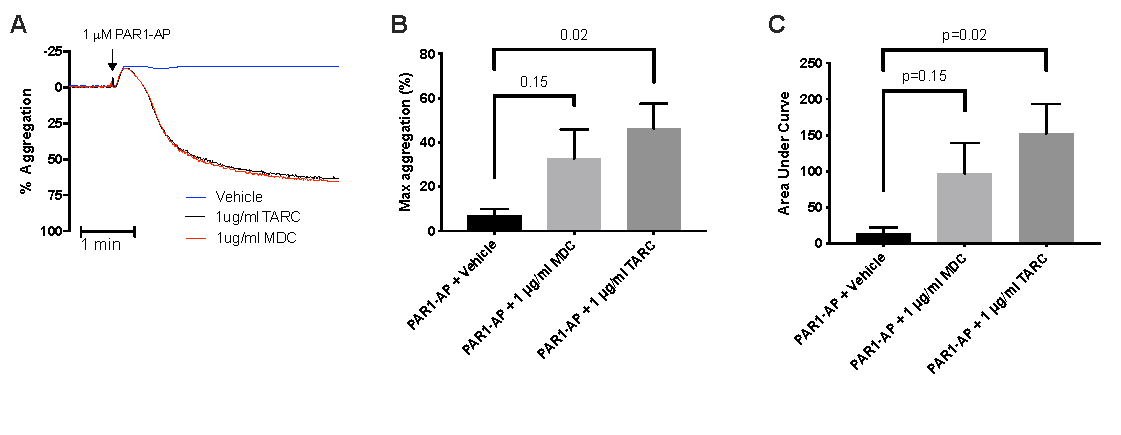
\includegraphics[width=0.85\linewidth]{figure/Chemokines/Layouts/MDC_TARC_aggregation_PAR1} 

}

\caption[The priming effect of the chemokines MDC and TARC on PAR1-AP induced platelet aggregation in washed platelets]{\textbf{The priming effect of the chemokines MDC and TARC on PAR1-AP induced platelet aggregation in washed platelets}. Washed platelets at 2x10\textsuperscript{8}/mL supplemented with apyrase were preincubated with MDC or TARC (5 min) before application of PAR1-AP-induced aggregation (5 mins). A) Raw aggregation trace comparing the effect of vehicle, 200 ng/mL MDC or 200 ng/mL TARC on PAR1-AP induced aggregation. B) Bar chart comparing the maximum PAR1-AP-mediated aggregation reached in the presence of vehicle, MDC or TARC. C) Bar chart comparing the area under the curve of PAR1-AP mediated aggregation trace in the presence of vehicle, MDC or TARC. Results analysed with a repeated measures one-way ANOVA with Dunnett's multiple comparisons. N=7. Mean+SEM displayed.}\label{fig:MDC-TARC-agg}
\end{figure}
\hypertarget{priming-effects-of-mdc-and-tarc-on-platelet-aggregation-in-prp}{%
\subsection{Priming effects of MDC and TARC on platelet aggregation in PRP}\label{priming-effects-of-mdc-and-tarc-on-platelet-aggregation-in-prp}}

Next, the priming effect of MDC and TARC was explored on platelet aggregation in PRP using plate aggregation, to see whether priming also occurs in the presence of plasma. Plate aggregation allows exploration of more conditions than LTA, therefore full concentration-response curves can be constructed. MDC and TARC were not able to potentiate the aggregation induced by increasing concentrations of PAR1-AP (Figure \ref{fig:MDC-TARC-agg-PRP}A). There was no difference in the pEC50 for comparing vehicle with MDC and TARC (Figure \ref{fig:MDC-TARC-agg-PRP}B).



\begin{figure}

{\centering 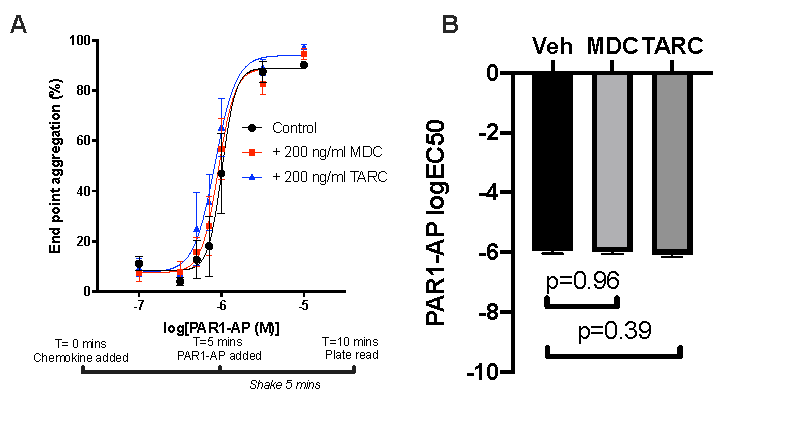
\includegraphics{figure/Chemokines/Layouts/MDC_TARC_PRP_plate_agg} 

}

\caption[The priming effect of the chemokines MDC and TARC on PAR1-AP induced platelet aggregation in PRP using plate aggregation]{\textbf{The priming effect of the chemokines MDC and TARC on PAR1-AP induced platelet aggregation in PRP using plate aggregation.} PRP supplemented with apyrase was preincubated with MDC or TARC (5 mins) before application of PAR1-AP and aggregation induced by a plate shaker (5 mins). A) PAR1-AP-induced platelet aggregation concentration-response curves in the presence of vehicle, 200 ng/mL MDC or 200 ng/mL TARC. N=7. B) Bar chart of the pEC50s of the PAR1-AP concentration response curve in the presence of vehicle, MDC or TARC. Results analysed using a repeated measures one-way ANOVA with Dunnett's multiple comparisons. N=7.}\label{fig:MDC-TARC-agg-PRP}
\end{figure}
\hypertarget{priming-effects-of-mdc-and-tarc-on-par1-ap-induced-integrin-ux3b1iibux3b23-activation-and-p-selectin-expression}{%
\subsection{\texorpdfstring{Priming effects of MDC and TARC on PAR1-AP induced integrin α\textsubscript{IIb}β\textsubscript{3} activation and P-selectin expression}{Priming effects of MDC and TARC on PAR1-AP induced integrin αIIbβ3 activation and P-selectin expression}}\label{priming-effects-of-mdc-and-tarc-on-par1-ap-induced-integrin-ux3b1iibux3b23-activation-and-p-selectin-expression}}

When a platelet becomes activated by an agonist, the integrin α\textsubscript{IIb}β\textsubscript{3} changes confirmation and is activated on the membrane of the platelet. This allows fibrinogen to bind and aggregation to occur. Following platelet activation, alpha granules fuse with the platelet plasma membrane and P-selectin becomes expressed on the plasma membrane. To assess whether MDC and TARC affect integrin α\textsubscript{IIb}β\textsubscript{3} activation and P-selectin expression, washed platelets were incubated with vehicle, 200 ng/ml MDC or TARC prior to PAR-AP stimulation. MDC enhanced integrin α\textsubscript{IIb}β\textsubscript{3} activation, with a leftward shift in the PAR1-AP concentration response curve (pEC50= -5.54 M (SEM 0.10 M) to -5.66 M (SEM 0.08 M), p=0.02). Preincubation with TARC had the same effect as MDC, left shifting the concentration-response curve (pEC50 = -5.54 M (SEM 0.11 M) to -5.64 M (SEM 0.11 M), p=0.01, Figure \ref{fig:MDC-TARC-integrin-pselectin}A). MDC and TARC did not cause a significant increase in the maximal integrin activation. As the concentration of PAR1-AP applied to the platelets gets higher, more P-selectin was exposed and therefore there was an increase in the MFI. The pEC50 for the PAR1-AP effect on P-selectin expression was -5.36 (SEM 0.07) (Figure \ref{fig:MDC-TARC-integrin-pselectin}B). Preincubation with 200 ng/ml MDC caused a small leftward shift in pEC50 to -5.44 (SEM 0.07) (MDC v vehicle, p=0.006), but preincubation with 200 ng/ml TARC did not alter the sensitivity to PAR1-AP. Together these results show that MDC and TARC are able to potentiate platelet activation mainly through integrin α\textsubscript{IIb}β\textsubscript{3}. In the absence of PAR1-AP, both MDC and TARC had a weak effect on integrin α\textsubscript{IIb}β\textsubscript{3} activation: increasing basal levels from a median fluorescence intensity (MFI) of 161 (SEM 20) to 222 (SEM 27) (vehicle v MDC, p=0.006) and to 285 ± 36 (vehicle v TARC, p=0.007) respectively (Figure \ref{fig:MDC-TARC-integrin-pselectin}C). This effect was specific to integrin α\textsubscript{IIb}β\textsubscript{3} as it was not seen with P-selectin.



\begin{figure}

{\centering 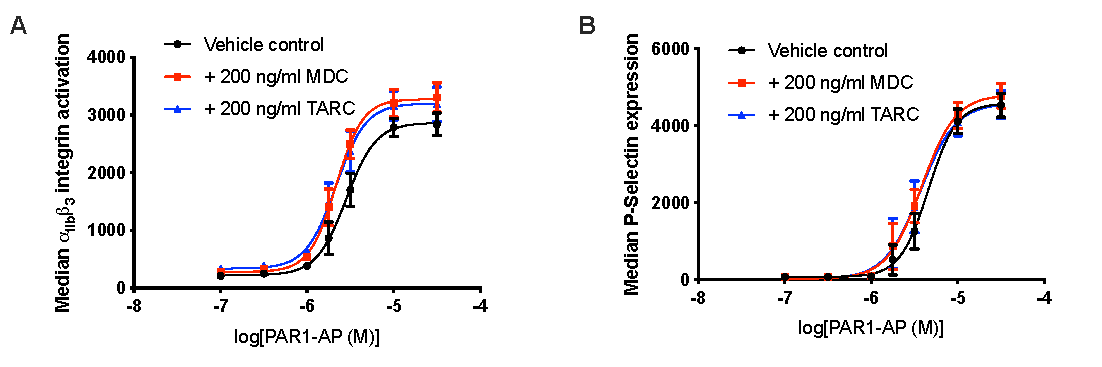
\includegraphics[width=0.7\linewidth]{figure/Chemokines/Layouts/P-selectin_integrin_MDC_TARC} 

}

\caption[The priming effect of the chemokines MDC and TARC on PAR1-AP induced α\textsubscript{IIb}β\textsubscript{3} activation and P-selectin expression]{\textbf{The priming effect of the chemokines MDC and TARC on PAR1-AP induced α\textsubscript{IIb}β\textsubscript{3} activation and P-selectin expression.} Washed platelets at 2x10\textsuperscript{7}/mL supplemented with apyrase were preincubated with MDC or TARC (5 mins) before application of PAR1-AP (5 mins). Integrin α\textsubscript{IIb}β\textsubscript{3} activation and P-selectin expression were measured using flow cytometry. A) The effect of vehicle, 200 ng/mL MDC or 200 ng/mL TARC on PAR1-AP induced α\textsubscript{IIb}β\textsubscript{3} activation measured as the median fluorescence intensity (AU). B) The effect of vehicle, MDC or TARC on PAR1-AP induced P-selectin expression measured using median fluorescence intensity (AU). pEC50s compared using a one-way ANOVA with Dunnett's multiple comparisons in Table \ref{tab:chemokines-integrin-pselectin} C) MDC and TARC alone increase integrin α\textsubscript{IIb}β\textsubscript{3} activation. Mean + SEM displayed. N=4.}\label{fig:MDC-TARC-integrin-pselectin}
\end{figure}


\begin{table}

\caption[Comparison of the effect of MDC and TARC on the pEC50 for PAR1-AP induced integrin activation and P-selectin expression]{\label{tab:chemokines-integrin-pselectin}\textbf{Comparison of the effect of MDC and TARC on the pEC50 for PAR1-AP induced integrin activation and P-selectin expression}. Estimate compared with a one-way ANOVA (N=4).}
\centering
\fontsize{9}{11}\selectfont
\begin{tabu} to \linewidth {>{\raggedright}X>{\raggedright}X>{\raggedright}X>{\raggedright}X>{\raggedright}X>{\raggedright}X>{\raggedright}X}
\toprule
Condition & Integrin activation pEC50 (M) & Integrin pEC50 SEM & Integrin P value & P-selectin pEC50 (M) & P-selectin pEC50 SEM & P-selectin p value\\
\midrule
Vehicle & -5.54 & 0.1 &  & -5.36 & 0.07 & \\
MDC & -5.66 & 0.08 & 0.019 & -5.44 & 0.07 & 0.006\\
TARC & -5.64 & 0.11 & 0.014 & -5.46 & 0.11 & 0.21\\
\bottomrule
\end{tabu}
\end{table}
\hypertarget{effects-of-mdc-and-tarc-on-ps-exposure}{%
\subsection{Effects of MDC and TARC on PS exposure}\label{effects-of-mdc-and-tarc-on-ps-exposure}}

When a platelet is activated by strong agonists, such as dual stimulation by collagen-related peptide (CRP) and thrombin, PS is translocated from the inner platelet membrane to the outer, thereby facilitating coagulation by providing binding sites for prothrombinase complex and supporting thrombin generation\textsuperscript{\protect\hyperlink{ref-Reddy2020}{149}}. MDC and TARC did not affect the overall percentage of annexin V positive platelets induced by CRP and thrombin (Figure \ref{fig:MDC-TARC-PS-exposure}).



\begin{figure}

{\centering 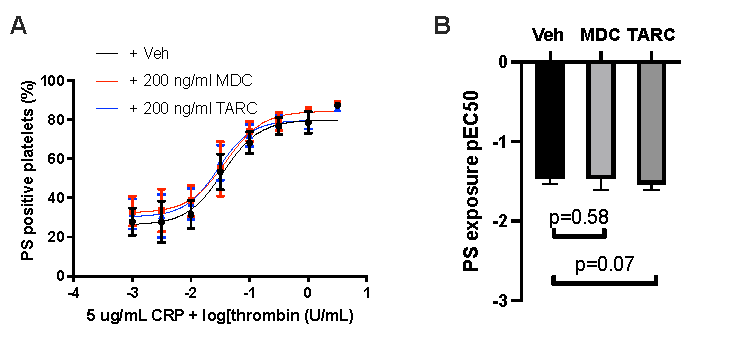
\includegraphics{figure/Chemokines/Layouts/MDC_TARC_PS_exposure_layout} 

}

\caption[The effect of the chemokines MDC and TARC on agonist induced PS exposure]{\textbf{The effect of the chemokines MDC and TARC on agonist induced PS exposure}. A) Washed platelets at 2x10\textsuperscript{7}/mL supplemented with indomethacin and apyrase were preincubated with vehicle, 200ng/mL MDC or 200 ng/mL TARC (5 mins) before application of CRP and increasing concentrations of thrombin (10 mins). PS exposure was measured using flow cytometry (N=4). B) Bar chart comparing the effect of vehicle, MDC or TARC on the pEC50s (M) of thrombin induced PS exposure. pEC50s were compared by a Friedman's test.}\label{fig:MDC-TARC-PS-exposure}
\end{figure}
\hypertarget{effects-of-mdc-and-tarc-alone-on-aggregation-in-washed-platelets}{%
\subsection{Effects of MDC and TARC alone on aggregation in washed platelets}\label{effects-of-mdc-and-tarc-alone-on-aggregation-in-washed-platelets}}

MDC and TARC were applied to washed platelets to determine whether they exert effects on platelet aggregation in the absence of an agonist. MDC and TARC did not cause platelet aggregation, however they did cause an upward deflection on the aggregation trace (Figure \ref{fig:MDC-TARC-wp-alone-aggregation}). This upward deflection is a reduction in light passing through the sample, indicating that the platelets may be undergoing shape change.



\begin{figure}

{\centering 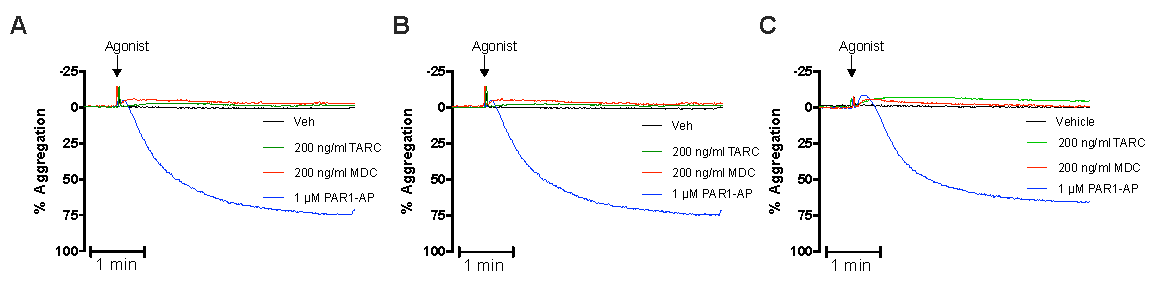
\includegraphics[width=0.9\linewidth]{figure/Chemokines/Layouts/MDC_TARC_alone_wp_aggregation} 

}

\caption[The effect of the chemokines MDC and TARC alone on aggregation in washed platelets]{\textbf{The effect of the chemokines MDC and TARC alone on aggregation in washed platelets}. A-C) Washed platelets at 2x10\textsuperscript{8}/mL supplemented with apyrase were stimulated with vehicle, 200ng/mL MDC, 200 ng/mL TARC or 1 uM PAR1-AP (5 mins). Aggregation was measured using light transmission aggregometry. Each graph is a representative trace from a separate donor}\label{fig:MDC-TARC-wp-alone-aggregation}
\end{figure}
\hypertarget{effects-of-mdc-and-tarc-alone-on-calcium-mobilisation}{%
\subsection{Effects of MDC and TARC alone on calcium mobilisation}\label{effects-of-mdc-and-tarc-alone-on-calcium-mobilisation}}

Calcium mobilisation was measured by using a fluorescent dye, Fura-2, which binds to intracellular calcium. Increasing concentrations of ADP were added to washed platelets as a positive control, where increasing calcium mobilisation was observed (\ref{fig:MDC-TARC-wp-calcium}A). MDC and TARC alone were also able to increase calcium mobilisation in a concentration-dependent manner (\ref{fig:MDC-TARC-wp-calcium}B), however caused a much smaller calcium response than ADP.



\begin{figure}

{\centering 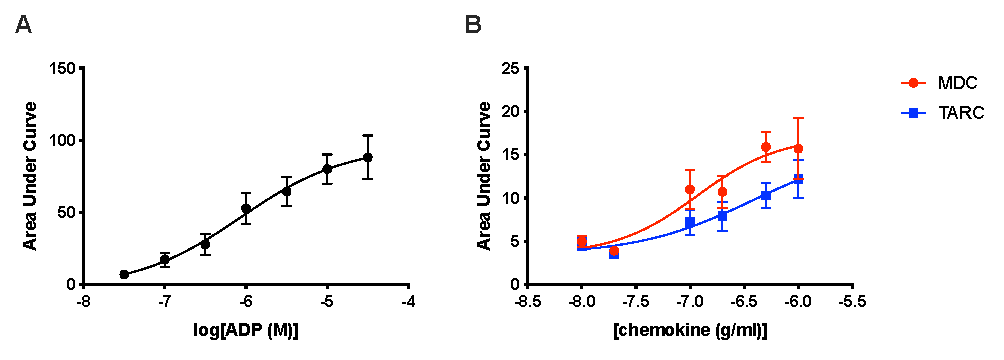
\includegraphics[width=0.9\linewidth]{figure/Chemokines/Layouts/MDC_TARC_calcium_wp} 

}

\caption[The effect of ADP and the chemokines MDC and TARC alone on calcium mobilisation in washed platelets.]{\textbf{The effect of ADP and the chemokines MDC and TARC alone on calcium mobilisation in washed platelets.} Washed platelets at 2x10\textsuperscript{8}/mL supplemented with indomethacin and apyrase were loaded with Fura-2. Platelets were stimulated with increasing concentrations of A) ADP or B) 200ng/mL MDC or 200 ng/mL TARC. Area under curve represents the free calcium and is ratio of fluorescence at wavelengths 340:380 nm.}\label{fig:MDC-TARC-wp-calcium}
\end{figure}
\hypertarget{mechanism-of-mdc-and-tarc-priming-in-washed-platelets}{%
\subsection{Mechanism of MDC and TARC priming in washed platelets}\label{mechanism-of-mdc-and-tarc-priming-in-washed-platelets}}

MDC and TARC activate the platelet receptor CCR4, which can reportedly couple to G\textsubscript{i/o}. PGE\textsubscript{1} inhibits platelets by acting at a G\textsubscript{s} coupled receptor, thereby increasing levels of cAMP and activating protein kinase A (PKA). PKA subsequently phosphorylates VASP. One mechanism by which MDC and TARC may therefore increase platelet function is by activating the G\textsubscript{i} pathway, which would oppose cAMP inhibition of platelet function. ADP acts at the P2Y\textsubscript{12} receptor which is G\textsubscript{i/o} coupled, therefore it reduces PGE\textsubscript{1} induced VASP phosphorylation. To explore whether MDC and TARC activate G\textsubscript{i} signaling, the effect of MDC and TARC on VASP phosphorylation in the presence and absence of PGE\textsubscript{1} was explored. PGE\textsubscript{1} increased the phosphorylation of VASP at both Ser\textsuperscript{157} and Ser\textsuperscript{239}. Figure \ref{fig:MDC-TARC-wp-WB-VASP} shows a representative blot from one donor. There was little evidence for an effect of MDC, TARC and ADP reducing basal VASP levels (Figure \ref{fig:MDC-TARC-wp-VASP-bar}A, C). As a positive control, ADP (10 µM) reduced the phosphorylation of VASP induced by 100 nM PGE\textsubscript{1} at both Ser\textsuperscript{239} by 62 \% SEM (18 \%) (ADP v vehicle, p=0.048, Figure \ref{fig:MDC-TARC-wp-VASP-bar}B) and at Ser\textsuperscript{157} by 44 \% (SEM 21 \%) (ADP v vehicle, p=0.048, Figure \ref{fig:MDC-TARC-wp-VASP-bar}D). In contrast, there was not strong evidence that MDC and TARC reduced the phosphorylation of VASP induced by 100 nM PGE1 at Ser\textsuperscript{239} or at Ser\textsuperscript{157} (Figures \ref{fig:MDC-TARC-wp-VASP-bar}B, D). This was also true for 10 nM and 30 nM PGE1 (data not shown). Phospho-VASP at Ser\textsuperscript{157} was also measured using flow cytometry (Figure \ref{fig:MDC-TARC-VASP-FACS}). PGE\textsubscript{1} increased phosphorylation of VASP in a concentration-dependent manner, with a pEC50 of -8.36 M (SEM 0.16 M). Pre-incubation with ADP shifted this response to the right to give a pEC50 of -6.95 M (SEM 0.17 M) (ADP v vehicle, p=0.002). MDC and TARC did not alter the PGE1 phosphorylation of VASP. Together, these results indicate that MDC and TARC do not signal through G\textsubscript{i}-coupled receptors in human platelets, or too weakly to detect using Western blotting or flow cytometry.



\begin{figure}

{\centering 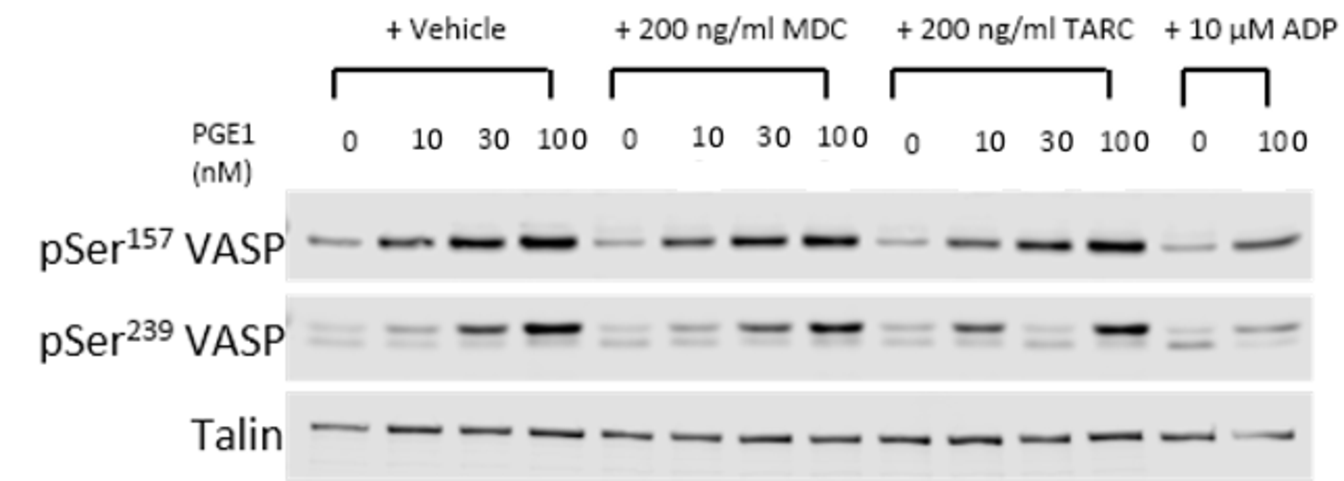
\includegraphics[width=0.55\linewidth]{figure/Chemokines/MDC_TARC_VASP_blot} 

}

\caption[A representative blot of the effect of MDC, TARC and ADP on PGE\textsubscript{1} stimulated phospho-VASP.]{\textbf{A representative blot of the effect of 200 ng/mL MDC, 200 ng/mL TARC and 10 uM ADP on phospho-VASP at Serine\textsuperscript{157} and Serine\textsuperscript{239} in the presence of increasing concentrations of PGE\textsubscript{1}}. Quantification is shown in Figure \ref{fig:MDC-TARC-wp-VASP-bar}.}\label{fig:MDC-TARC-wp-WB-VASP}
\end{figure}


\begin{figure}

{\centering 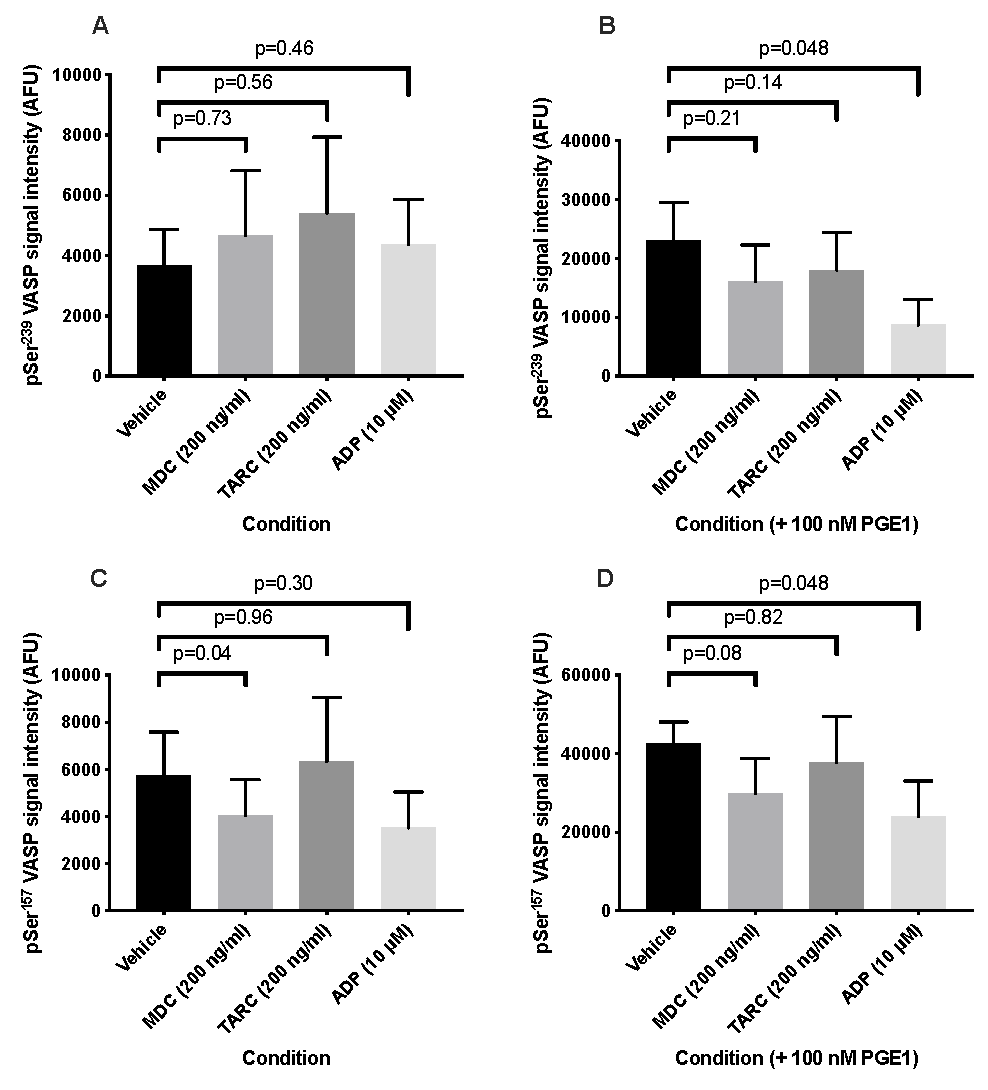
\includegraphics{figure/Chemokines/Layouts/MDC_TARC_WB_VASP} 

}

\caption[Quantification of the effect of MDC, TARC and ADP on PGE\textsubscript{1} stimulated phospho-VASP.]{\textbf{Quantification of the effect of MDC, TARC and ADP on PGE\textsubscript{1} stimulated phospho-VASP.} Bar charts of the effect of 200 ng/mL MDC, 200 ng/mL TARC and 10 uM ADP on phospho-VASP at A) Serine 239 in the absence of PGE\textsubscript{1}, B) Serine 239 in the presence of 100 nM PGE\textsubscript{1}, C) Serine 157 in the absence of PGE\textsubscript{1}, D) Serine 157 in the presence of 100 nM PGE\textsubscript{1}. N=4. Results analysed with a repeated measures one-way ANOVA with Dunnett's Multiple comparisons.}\label{fig:MDC-TARC-wp-VASP-bar}
\end{figure}


\begin{figure}

{\centering 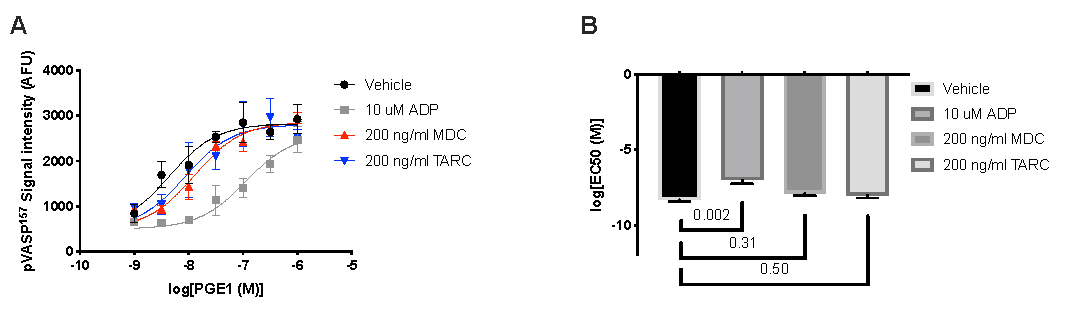
\includegraphics[width=0.9\linewidth]{figure/Chemokines/Layouts/MDC_TARC_VASP_FACS_logec50} 

}

\caption[The effect of the chemokines MDC and TARC on phospho-VASP levels using flow cytometry]{\textbf{The effect of the chemokines MDC and TARC on phospho-VASP levels using flow cytometry.} A) Washed platelets at 1x10\textsuperscript{8}/mL were supplemented with indomethacin and apyrase. Platelets were preincubated with vehicle, 200ng/mL MDC, 200 ng/mL TARC or 10 uM ADP (5 mins) before application of increasing concentrations of PGE\textsubscript{1} (5 mins). Phospho-VASP at Ser\textsuperscript{157} was measured using flow cytometry (N=3). B) Bar chart of the pEC50s of each concentration response curve from A. pEC50s were compared using a one-way ANOVA with Dunnett's multiple comparisons.}\label{fig:MDC-TARC-VASP-FACS}
\end{figure}
\hypertarget{mechanisms-of-the-effect-of-mdc-on-platelet-aggregation-in-prp}{%
\subsection{Mechanisms of the effect of MDC on platelet aggregation in PRP}\label{mechanisms-of-the-effect-of-mdc-on-platelet-aggregation-in-prp}}

The mechanism by which these chemokines cause platelet aggregation in PRP was further characterised just using MDC. MDC-induced platelet aggregation was explored using various inhibitors. To test that the antagonists used were specific, they were first applied to PAR1-AP. As expected, the CCR4 antagonist AZD-2098 did not affect PAR1-AP platelet aggregation. The G\textsubscript{q} inhibitor YM-254890 inhibited PAR1-AP induced platelet aggregation (Figures \ref{fig:MDC-PRP-agg-bar}A, B). Y27632 inhibited the G\textsubscript{12/13} mediated shape change induced by low concentrations of PAR1-AP (0.75 uM) due inhibiting rho-associated protein kinase (ROCK) (data not shown).

The effects of these inhibitors on MDC-induced aggregation were then explored. MDC by itself was able to consistently cause over 60\% aggregation in PRP. The CCR4 inhibitor AZD-2098 was able to reduce this aggregation, but only at 50 uM (Figures \ref{fig:MDC-PRP-agg-bar}C, \ref{fig:MDC-PRP-agg-trace}A, B). The G\textsubscript{q} inhibitor YM-254890 was able to reduce the maximum aggregation induced by MDC (Figure \ref{fig:MDC-PRP-agg-bar}C, Figure \ref{fig:MDC-PRP-agg-trace}C), suggesting CCR4 couples to G\textsubscript{q}. Y27632 did not affect aggregation induced by MDC, suggesting that this aggregation is not dependent on G\textsubscript{12/13} and ROCK (Figure \ref{fig:MDC-PRP-agg-bar}D, \ref{fig:MDC-PRP-agg-trace}D). Application of MDC to PRP did not cause shape change.



\begin{figure}

{\centering 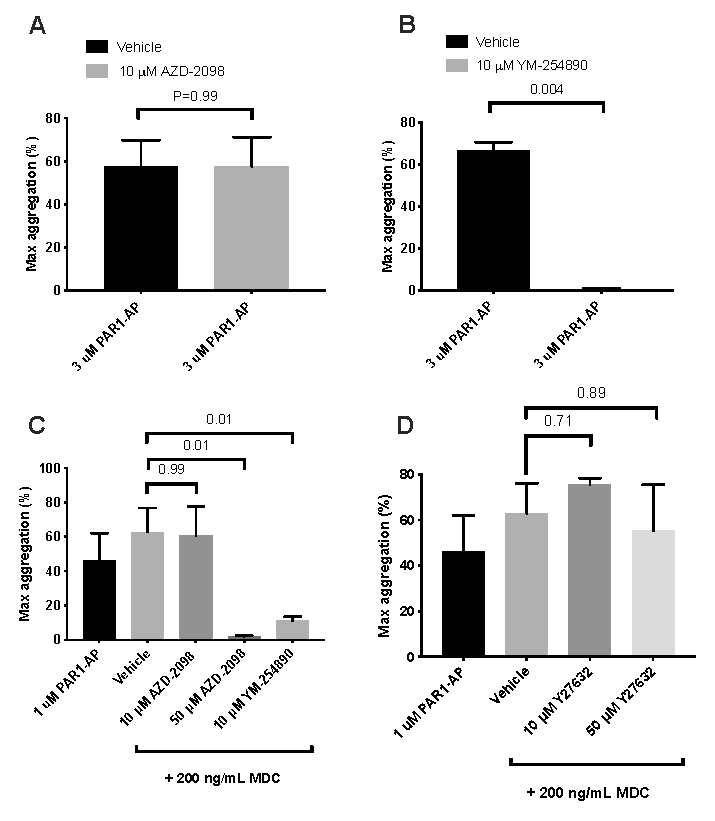
\includegraphics[width=0.95\linewidth]{figure/Chemokines/Layouts/PAR1_MDC_inhibitors_aggregation} 

}

\caption[The effect of inhibitors on PAR1-AP and MDC induced aggregation in PRP.]{\textbf{The effect of inhibitors on PAR1-AP and MDC induced aggregation in PRP.} Platelet rich plasma (PRP) supplemented with apyrase was incubated for 5 minutes with the antagonist indicated, followed by stimulation by PAR1-AP or MDC. A) Effect of 10 uM AZD-2098 (CCR4 antagonist) on maximal aggregation induced by PAR1-AP B) Effect of 10 uM YM-254890 (G\textsubscript{q} inhibitor) on maximal aggregation induced by PAR1-AP C) Effect of AZD-2098 and YM-254890 on aggregation induced by 200 ng/mL MDC D) Effect of the ROCK inhibitor Y27632 on aggregation induced by 200 ng/mL MDC Results are analysed with a paired two-tailed t-test or repeated measures one-way ANOVA with Dunnett's Multiple comparisons. N=3-5.}\label{fig:MDC-PRP-agg-bar}
\end{figure}


\begin{figure}

{\centering 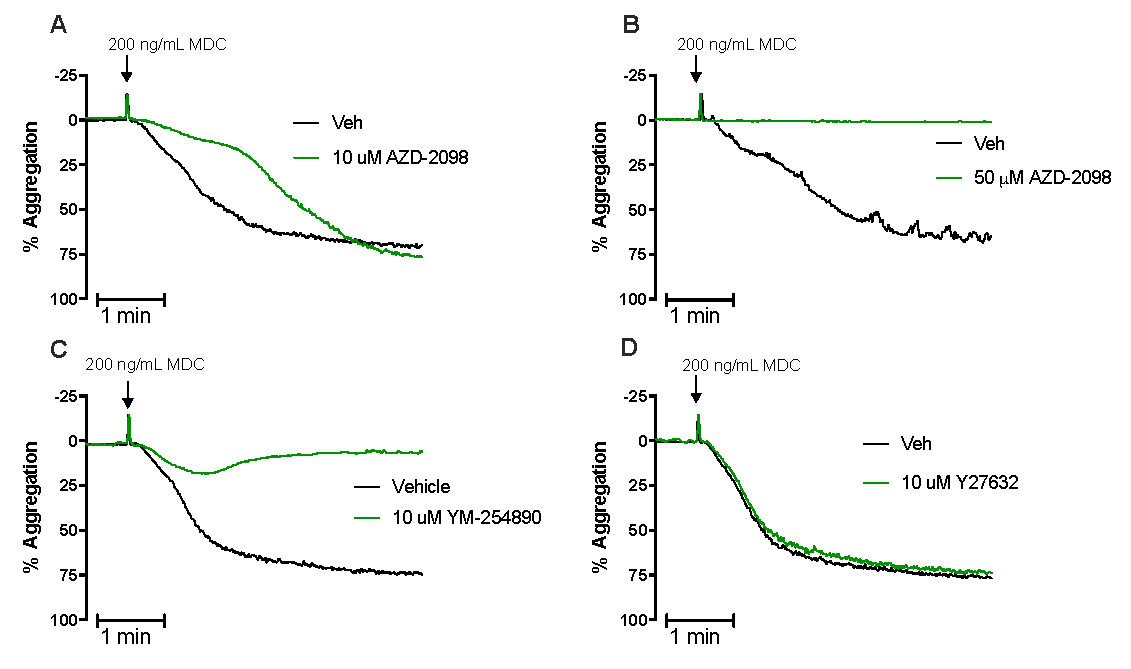
\includegraphics[width=0.95\linewidth]{figure/Chemokines/Layouts/MDC_inhibitors_aggregation_traces} 

}

\caption[Aggregation traces of the effect of inhibitors on MDC induced platelet aggregation in PRP.]{\textbf{Aggregation traces of the effect of inhibitors on MDC induced platelet aggregation in PRP.} Representative aggregation traces of platelet rich plasma (PRP) supplemented with apyrase, incubated with A) 10 uM CCR4 antagonist AZD-2098 B) 50 uM AZD-2098 C) 10 uM G\textsubscript{q} inhibitor YM-254890 D) 10 uM ROCK inhibitor Y27632, followed by addition of 200 ng/mL MDC.}\label{fig:MDC-PRP-agg-trace}
\end{figure}
\hypertarget{two-sample-mendelian-randomisation-to-assess-the-role-of-mdc-ccl22-and-tarc-ccl17-in-disease}{%
\subsection{Two sample Mendelian randomisation to assess the role of MDC (CCL22) and TARC (CCL17) in disease}\label{two-sample-mendelian-randomisation-to-assess-the-role-of-mdc-ccl22-and-tarc-ccl17-in-disease}}

To estimate potential causal relationships bewteen circulating levels of MDC and TARC and disease, a two sample MR was performed using pQTL data for these chemokines and available disease outcome data. Results are displayed for estimates where p\textless0.05, however due to multiple testing, the p-value threshold was adjusted to 2.2x10\textsuperscript{-4}. Results are presented as the change in outcome per SD higher protein. There was evidence from the Wald ratio MR that higher MDC had a causal effect on three outcomes: high cholesterol (Effect size = 0.22 SD, SE = 0.02, p=2.2x10\textsuperscript{-26}), DVT (Effect size = 0.22, SE 0.021, p=2.2x10\textsuperscript{-26}) and pulmonary embolism (Effect size = 0.33, SE 0.08, p=2.0x10\textsuperscript{-5}). There was not strong evidence for an effect of higher levels of TARC on any of the included outcomes. Results of the two sample MR are shown for MDC and TARC in tables \ref{tab:MDC-disease-MR} and \ref{tab:TARC-disease-MR}.


\begin{landscape}\begin{table}

\caption{\label{tab:MDC-disease-MR}Estimates for the effect of MDC on disease outcomes using two sample Mendelian randomization}
\centering
\fontsize{9}{11}\selectfont
\begin{tabu} to \linewidth {>{\raggedright}X>{\raggedright\arraybackslash}p{5cm}>{\raggedright}X>{\raggedright}X>{\raggedright}X>{\raggedright}X>{\raggedright}X}
\toprule
Protein & Outcome trait & N SNP (rsID) & Method & Effect sie & Standard error & P value\\
\midrule
MDC/CCL22 & Non-cancer illness code self-reported: high cholesterol & 1 (rs77542162) & Wald ratio & 0.2224 & 0.0209 & 2.2e-26\\
MDC/CCL22 & Non-cancer illness code self-reported: deep venous thrombosis (dvt) & 1 (rs77542162) & Wald ratio & 0.2936 & 0.0512 & 9.81e-09\\
MDC/CCL22 & Non-cancer illness code self-reported: pulmonary embolism (with or without) dvt & 1 (rs77542162) & Wald ratio & 0.3308 & 0.0775 & 1.969e-05\\
MDC/CCL22 & Forced expiratory volume in 1-second (FEV1) & 1 (rs77542162) & Wald ratio & 0.0312 & 0.0084 & 0.0001961\\
MDC/CCL22 & Forced vital capacity (FVC) & 1 (rs77542162) & Wald ratio & 0.0285 & 0.0079 & 0.0003201\\
\addlinespace
MDC/CCL22 & Eye problems or disorders: Glaucoma & 1 (rs77542162) & Wald ratio & 0.2292 & 0.0654 & 0.000457\\
MDC/CCL22 & Diagnoses - main ICD10: M16 Coxarthrosis [arthrosis of hip] & 1 (rs77542162) & Wald ratio & 0.2217 & 0.0648 & 0.0006186\\
MDC/CCL22 & Non-cancer illness code self-reported: gout & 1 (rs77542162) & Wald ratio & -0.4045 & 0.1237 & 0.001075\\
MDC/CCL22 & Non-cancer illness code self-reported: hypothyroidism or myxoedema & 1 (rs77542162) & Wald ratio & 0.1203 & 0.0381 & 0.001607\\
MDC/CCL22 & Schizophrenia & 1 (rs77542162) & Wald ratio & -0.1477 & 0.048 & 0.002086\\
\addlinespace
MDC/CCL22 & Systolic blood pressure automated reading & 1 (rs77542162) & Wald ratio & -0.0283 & 0.0099 & 0.004246\\
MDC/CCL22 & Alcohol intake frequency & 1 (rs77542162) & Wald ratio & -0.04 & 0.0143 & 0.005124\\
MDC/CCL22 & Non-cancer illness code self-reported: osteoporosis & 1 (rs77542162) & Wald ratio & 0.1593 & 0.0665 & 0.01655\\
MDC/CCL22 & Diagnoses - main ICD10: K80 Cholelithiasis & 1 (rs77542162) & Wald ratio & -0.1965 & 0.0826 & 0.01731\\
MDC/CCL22 & Fracture resulting from simple fall & 1 (rs77542162) & Wald ratio & 0.0528 & 0.0236 & 0.02527\\
\addlinespace
MDC/CCL22 & Cancer code self-reported: small intestine or small bowel cancer & 1 (rs77542162) & Wald ratio & 0.5966 & 0.2745 & 0.02976\\
MDC/CCL22 & Eye problems or disorders: Cataract & 1 (rs77542162) & Wald ratio & 0.0991 & 0.0487 & 0.04163\\
MDC/CCL22 & Diagnoses - main ICD10: R04 Haemorrhage from respiratory passages & 1 (rs77542162) & Wald ratio & 0.2189 & 0.1094 & 0.04552\\
MDC/CCL22 & Diagnoses - main ICD10: I80 Phlebitis and thrombophlebitis & 1 (rs77542162) & Wald ratio & 0.2269 & 0.1145 & 0.04755\\
\bottomrule
\end{tabu}
\end{table}
\end{landscape}

\begin{landscape}\begin{table}

\caption{\label{tab:TARC-disease-MR}Estimates for the effect of TARC on disease outcomes using two sample Mendelian randomization}
\centering
\fontsize{10}{12}\selectfont
\begin{tabu} to \linewidth {>{\raggedright}X>{\raggedright\arraybackslash}p{4cm}>{\raggedright}X>{\raggedright}X>{\raggedright}X>{\raggedright}X>{\raggedright}X}
\toprule
Protein & Outcome trait & N SNP (rsID) & Method & Effect sie & Standard error & P value\\
\midrule
TARC/CCL17 & Rheumatoid arthritis & 2 (rs983545, rs222846) & Inverse variance weighted & 0.1015 & 0.0386 & 0.00851\\
TARC/CCL17 & Anorexia nervosa & 2 (rs983545, rs222846) & Inverse variance weighted & 0.2182 & 0.0845 & 0.009826\\
TARC/CCL17 & Non-cancer illness code self-reported: gastro-oesophageal reflux (gord) or gastric reflux & 2 (rs983545, rs222846) & Inverse variance weighted & 0.003 & 0.0012 & 0.01172\\
TARC/CCL17 & Systemic lupus erythematosus & 2 (rs983545, rs222846) & Inverse variance weighted & 0.2716 & 0.114 & 0.01717\\
TARC/CCL17 & Ischemic stroke & 2 (rs983545, rs222846) & Inverse variance weighted & -0.081 & 0.0373 & 0.02999\\
\addlinespace
TARC/CCL17 & Red blood cell count & 2 (rs983545, rs222846) & Inverse variance weighted & -0.0116 & 0.0058 & 0.04445\\
\bottomrule
\end{tabu}
\end{table}
\end{landscape}
\hypertarget{discussion-2}{%
\section{Discussion}\label{discussion-2}}

This study explored the effects of the chemokines MDC and TARC on platelet function and signalling. Evidence suggested that MDC and TARC were able to potentiate platelet function induced by the agonist PAR1-AP in washed platelets. There was not strong evidence that this potentiation was mediated by a G\textsubscript{i/o}-coupled receptor. Functional experiments indicated that MDC and TARC are not only able to prime platelets, but that they are also able to cause a small calcium response and platelet shape change when applied alone in washed platelets. Experiments in PRP indicated that MDC is able to cause full aggregation and that this is due to the CCR4 receptor, and that this is G\textsubscript{q} coupled. Two sample MR was performed to estimate the causal effect of higher levels of MDC and TARC on disease. These results suggested that higher levels of MDC increased the risk of DVT and PE. These effects could be due to activation of platelets.

Previous studies have attempted to explore the effects of MDC and TARC on platelet function. There is evidence that MDC and TARC potentiate ADP-induced aggregation\textsuperscript{\protect\hyperlink{ref-Gear2001}{144}}. The current study provides evidence that this is also the case with PAR1-AP, therefore this effect is not agonist specific. MDC and TARC alone have been shown to elicit a calcium response, but only in PRP can aggregation occur\textsuperscript{\protect\hyperlink{ref-Kowalska2000}{78}}. This is likely due to components in PRP such as arachidonic acid or the presence of other platelet primers such as IGF-1. The current chapter confirmed these findings, where only shape change was achieved in washed platelets, but in PRP MDC could induce aggregation. As well as confirming previous findings, this chapter provided some novel observations. For example, this chapter explored whether MDC and TARC can potentiate PS exposure. There was no evidence that MDC and TARC could potentiate the procoagulant effects induced by CRP and thrombin. This may be because the signalling elicited by MDC and TARC may not be strong enough to affect PS exposure.

Platelets express chemokine receptors as they are also key cells in inflammation and host defense\textsuperscript{\protect\hyperlink{ref-Clemetson2000}{143}}. MDC and TARC can also cause activation of platelets, thereby demonstrating the close link between inflammation and haemostasis\textsuperscript{\protect\hyperlink{ref-Gear2003}{37}}.

As well as functional effects, this chapter aimed to assess whether effects are due to the CCR4 receptor and the downstream signalling involved. It has been reported that MDC inhibits calcium currents in HEK293 cells and barium currents dorsal root ganglia neurones and is therefore G\textsubscript{i/o} coupled\textsuperscript{\protect\hyperlink{ref-Oh2002}{151}}. MDC and TARC were not able to reduce VASP phosphorylation induced by PGE1, suggesting that the effects are not via G\textsubscript{i/o} in platelets. It is possible that this experiment was not sensitive enough to detect the reduction in VASP phosphorylation, as ADP did not reduce VASP levels as much as previous reports\textsuperscript{\protect\hyperlink{ref-Hezard2005}{60}}. Another study suggested that CCR4 is coupled to G\textsubscript{q} due to the calcium response observed by MDC\textsuperscript{\protect\hyperlink{ref-Kowalska2000}{78}}. Inhibiting G\textsubscript{q} coupling in the current study inhibited the aggregation induced by MDC. It is therefore likely that CCR4 couples to G\textsubscript{q}.

MDC and TARC have been implicated in cardiovascular disease such as atherosclerosis\textsuperscript{\protect\hyperlink{ref-Weber2004}{152}}, but experiments focusing on the effect of MDC and TARC on platelet function have not used genetic epidemiology to explore whether genetic variants which lead to alterations in the levels of circulating MDC and TARC in the plasma are associated with an increased risk of disease. As MDC and TARC can activate platelets, the effect of MDC and TARC on disease was explored using two sample MR. The SNP that was associated with levels of MDC, rs77542162, was also associated with increased risk of DVT and pulmonary embolism. This effect may occur due to increased platelet priming by higher levels of MDC. Patients at risk of developing VTE have a hypercoagulant state and are prescribed anticoagulants to reduce the risk. Experiments indicated that MDC could not potentiate PS exposure, a marker of coagulation, therefore suggesting that MDC does not increaes the risk through an increase in coagulation. Further experiments are required to determine how MDC could mediate the risk of VTE. Despite the evidence for a causal effect, it is possible that this SNP could affect the outcome through routes other than through the exposure (horizontal pleiotropy). For example, the SNP could also be associated with increased in number of red blood cells, thereby increased risk of VTE. This is also reflected by other outcomes being related to increased levels of MDC such as forced vital capacity (FVC). As there is only one SNP, sensitivity analyses cannot be performed to test this. Further analyses such as a colocalisation analysis could help determine whether the relationship between MDC and DVT/PE is causal as this method estimates whether an exposure and an outcome share a causal top signal in a particular genomic region\textsuperscript{\protect\hyperlink{ref-Giambartolomei2014}{153}}.

This chapter has provided evidence for a an effect of MDC and TARC on platelet function and indicated possible mechanisms of effect. As mentioned in the introduction of the current chapter, there is evidence that patients with obesity have higher circulating levels of MDC\textsuperscript{\protect\hyperlink{ref-Safa2016}{142}}, however the effect of BMI and levels of these chemokines needs to assessed in a larger cohort and using a causal framework. The SOMAScan proteomics panel detects these circulating chemokines, therefore further exploration of the effect of BMI on these chemokines will be presented in Chapter \ref{BMI-protein-MR} by using one sample MR and Chapter \ref{BMI-protein-RCT} which utilises a weight loss randomised control trial.

\hypertarget{conclusions}{%
\subsection{Conclusions}\label{conclusions}}

Overall, this chapter provided evidence that the chemokines MDC and TARC potentiate platelet aggregation induced by PAR1-AP. On their own in washed platelets, a small calcium response can be observed as well as shape change, but PRP is required to observe full aggregation. Signalling experiments suggest MDC and TARC act at the CCR4 receptor on platelets, and that G\textsubscript{q} coupling is responsible for the functional effects observed. There was evidence that higher MDC may have a causal effect on DVT and PE. MDC may therefore be a biomarker for venous thromboembolism. Further work is required to determine signalling, and further cohort studies would be useful to confirm effects of MDC on DVT and PE.

\hypertarget{BMI-protein-MR}{%
\chapter{Exploring the plasma proteome as a link between adiposity and platelet function: Observational and Mendelian randomization estimates}\label{BMI-protein-MR}}

The work within this chapter has been published in the International Journal of Obesity\textsuperscript{\protect\hyperlink{ref-Goudswaard2021}{154}}. I am the first author of the publication; I performed all analyses, created all figures and tables and wrote the manuscript.

Supplementary Tables 1-10 can be found here \url{https://github.com/lucygoudswaard/mythesis/blob/master/index/figure/BMI_protein_INTERVAL/BMI_protein_supplementary_Tables.xlsx}

\hypertarget{introduction}{%
\section{Introduction}\label{introduction}}

The previous chapters (Chapter \ref{BMI-platelets-INTERVAL} and Chapter \ref{BMI-platelets-clinic}) have provided evidence that higher body mass index raises immature platelet count and alters levels of platelet proteins which are important in platelet activation. As well as this, chapter \ref{chemokine-platelets} indicated that application of MDC and TARC on platelets \emph{ex vivo} leads to platelet activation. Despite this evidence, it is unclear how a higher BMI leads to an increased risk of thrombosis, in particular an increase in platelet production and changes in platelet signalling proteins. It is possible that molecules which circulate in the blood may be mediating this effect as platelets also circulate in the blood and blood vessels are the site of thrombi. Previous studies have largely focused on the impact of higher BMI on the lipidome including traits such as cholesterol and triglycerides in lipoprotein subtypes (e.g.~low-density lipoprotein (LDL) and high-density lipoprotein (HDL) particles)\textsuperscript{\protect\hyperlink{ref-Bell2018a}{31},\protect\hyperlink{ref-Wurtz2014}{32}} and on inflammatory molecules such as C-reactive protein (CRP)\textsuperscript{\protect\hyperlink{ref-Wurtz2014}{32},\protect\hyperlink{ref-Timpson2011}{87}}. Fewer studies have explored the effect of adiposity on the circulating proteome profile\textsuperscript{\protect\hyperlink{ref-Cominetti2018}{93}}.

A benefit of studying the systematic effects of BMI on the circulating proteome is that proteins are often more suitable pharmacological targets than metabolites. Efforts to study the effect of BMI on the proteome have generally been in an observational framework\textsuperscript{\protect\hyperlink{ref-Cominetti2018}{93}}. It is estimated that 25\% of proteins in the human proteome circulate in blood\textsuperscript{\protect\hyperlink{ref-Gold2012}{92}}, which is important as the majority of druggable targets are such proteins\textsuperscript{\protect\hyperlink{ref-Imming2006}{94}}. Studying the effect of BMI on a large set of proteins has only recently become possible with newly developed proteomic technologies such as the SomaLogic platform, with the ability to quantify enzymes, protein kinases and transport proteins with unprecedented sensitivity\textsuperscript{\protect\hyperlink{ref-Rohloff2014}{155}}. Utilisation of SomaLogic within a trial or cohort setting has recently become more widespread, such as within the INTERVAL study, a UK cohort of blood donors\textsuperscript{\protect\hyperlink{ref-Sun2018}{34}}. There is evidence that proteins which change as a result of a higher BMI may contribute to thrombosis (ref Andrei's paper): identification of such proteins is important in understanding how higher BMI causes disease and to identify targets which may benefit from pharmacological intervention. It is possible that proteins that are altered by BMI may contribute to thrombosis by activating platelets (Chapter \ref{chemokine-platelets}).

In this chapter, the aim is to measure associations between adiposity and the human proteome and to also estimate the underlying effects in a causal framework (Figure \ref{fig:BMI-protein-graphic-INT}). Using data on 2737 participants from INTERVAL, the effects of BMI on 4034 (3622 unique) plasma protein traits will be estimated in both observational and MR frameworks. The specific effect of BMI on platelet proteins will be explored, as well as a disease enrichment analysis.



\begin{figure}

{\centering \includegraphics[width=0.9\linewidth]{figure/BMI_protein_INTERVAL/Thesis_graphic_overview_BMI_protein_CVD} 

}

\caption[Schematic of the associations explored in /\textsuperscript{\protect\hyperlink{ref-ref}{\textbf{ref?}}}(BMI-protein-MR).]{\textbf{Schematic of the associations explored in Chapter \ref{BMI-protein-MR}.} This chapter explores the causal effect of BMI on the plasma proteome and explores whether these changes might contribute to cardiovascular diseases. Figure made using BioRender.com.}\label{fig:BMI-protein-graphic-INT}
\end{figure}
\hypertarget{methods-2}{%
\section{Methods}\label{methods-2}}

\hypertarget{study-population-2}{%
\subsection{Study population}\label{study-population-2}}

The present study was conducted on a random subset of participants from INTERVAL who had basic phenotype data and plasma proteins measured by SomaLogic. This included up to 2737 participants mostly of European descent across analyses described below. More details of the INTERVAL study can be found in Chapter \ref{BMI-platelets-INTERVAL} in section \ref{INTERVAL-study}.

\hypertarget{measurement-of-circulating-proteins}{%
\subsection{Measurement of circulating proteins}\label{measurement-of-circulating-proteins}}

Plasma proteins were measured in INTERVAL participants at baseline (before randomisation of assignment to the time interval between blood donation) using the SomaScan® by SomaLogic\textsuperscript{\protect\hyperlink{ref-Sun2018}{34}}. This platform uses 4034 modified nucleotides known as Slow Off-rate Modified Aptamers (SOMAmers) which make direct contact with proteins, enabling detection of 3622 unique proteins or protein complexes and quantifies them using a DNA microarray\textsuperscript{\protect\hyperlink{ref-Rohloff2014}{155}}. Separate SOMAmers can bind to isoforms of the same protein, but can also bind to the same protein at different sites (which can be impacted by post-translational modifications or complexes formed with other proteins). All 4034 SOMAmers were therefore included. The extensive number of proteins measured, with no missingness and in a cohort of 2737 participants, provides a rich proteomic dataset. The proteins were measured in relative fluorescence units (RFUs) and quality control (QC) was performed as described by Sun et al.\textsuperscript{\protect\hyperlink{ref-Sun2018}{34}}. There was no missingness across protein variables. The proteomic data used had been pre-adjusted (using linear regression) for age, sex, duration between blood draw and sample processing (1 day or less vs \textgreater1 day), and the first three genetic principal components, with the residuals inverse normal rank transformed. All following analyses use this `pre-adjusted' data as input.

\hypertarget{statistical-analyses}{%
\subsection{Statistical analyses}\label{statistical-analyses}}

The population characteristics of INTERVAL participants with SomaLogic data who were included in this study (N range: 2422 to 2737 due to missing data for covariables) were compared to those INTERVAL participants who were not included (N range: 27174 to 30721) to assess generalisability of any BMI-protein associations to the wider INTERVAL sample. Population characteristics evaluated were age, sex, weight, height, BMI, smoking frequency, and alcohol intake. Differences in population characteristics among the two INTERVAL sub-sets were tested by a two-sided t-test for continuous traits and a two-sided Chi-square test for categorical variables. Observational analyses were conducted using linear regression to examine associations between BMI (in normalized standard deviation (SD) units based on a rank normal transformation (rntransform() from ``moosefun'' package \url{https://github.com/hughesevoanth/moosefun}) and each standardised protein trait as a dependent (outcome) variable. Two linear models were used (using lm() function from R ``stats'' package): 1) adjusted for age and sex and 2) additionally adjusted for smoking and alcohol consumption (each as an ordered categorical variable). Given that the procedure which generates the ``pre-adjusted'' data (adjustment for covariables before rank normal transformation of proteins) can reintroduce correlations\textsuperscript{\protect\hyperlink{ref-Pain2018}{156}}, age and sex are again used as covariables here. The estimates derived from models 1) and 2) therefore reflect the normalized SD-unit difference in each protein trait per normalized SD-unit (4.8 kg/m\textsuperscript{2}) higher BMI. Associations of covariables with BMI and protein traits were also examined using linear regression.

A Shapiro-Wilk test was used to confirm whether the GRS showed a normal distribution. MR analyses were conducted using two-stage least squares (2SLS) regression models with robust standard errors, using the systemfit function as part of the systemfit package\textsuperscript{\protect\hyperlink{ref-Henningsen2007}{110}}, with measured BMI in SD units and the GRS for BMI as the instrumental variable. These MR estimates reflect the normalized SD-unit difference in each protein trait per normalized SD-unit (4.8 kg/m\textsuperscript{2}) higher BMI. Estimates are reported from the direct linear associations between BMI and proteins as ``observational'' estimates and those from the 2SLS causal effect estimates as ``MR estimates''. Agreement between observational and MR estimates was examined using a separate linear regression. This was performed: 1) for all proteins, and 2) excluding the proteins that fell below our P-value reference point for strong evidence (defined below) to examine whether agreement is limited to ``top hits'' or applies throughout the effect distribution. Agreement between observational estimates and MR estimates would suggest that there are causal effects of BMI across the general proteome, with differences in estimates suggesting confounding of observational estimates.

To account for multiple testing, a Bonferroni correction was used to adjust results. This was informed by the correlation between proteins, adjusting only for the estimated number of independent traits (Figure \ref{fig:Corr-mat-proteins}). Correlation was assessed by a Spearman's correlation matrix. From a starting number of 4034, the number of independent proteins was 3655 (using a correlation cut-off of r = 0.8 or tree cut height = 0.2 between proteins, Figure \ref{fig:Dend-proteins}), dendrogram made using ``iPVs'' package \url{https://github.com/hughesevoanth/iPVs}). A Bonferroni adjusted P-value of 0.05/3655 = 1.4x10\textsuperscript{-5} was utilised to indicate strong evidence in this sample. Full results are presented in the supplementary material.



\begin{figure}

{\centering 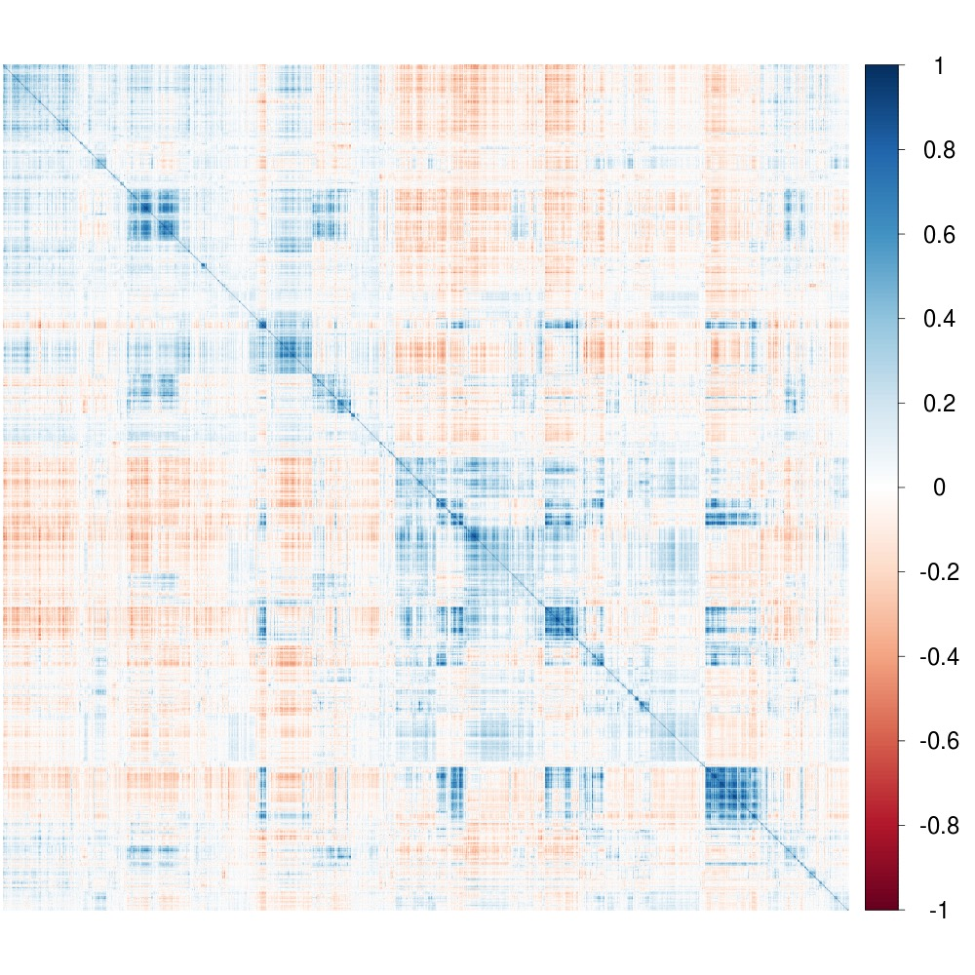
\includegraphics[width=0.9\linewidth]{figure/BMI_protein_INTERVAL/Correlation_matrix_proteins} 

}

\caption[Correlation matrix of all protein traits analysed by SomaLogic]{\textbf{Correlation matrix of all protein traits analysed by SomaLogic (4,034)}. The colour corresponds to the correlation coefficient ranging from 1 (dark blue) to -1 (dark red).}\label{fig:Corr-mat-proteins}
\end{figure}
\blandscape



\begin{figure}

{\centering 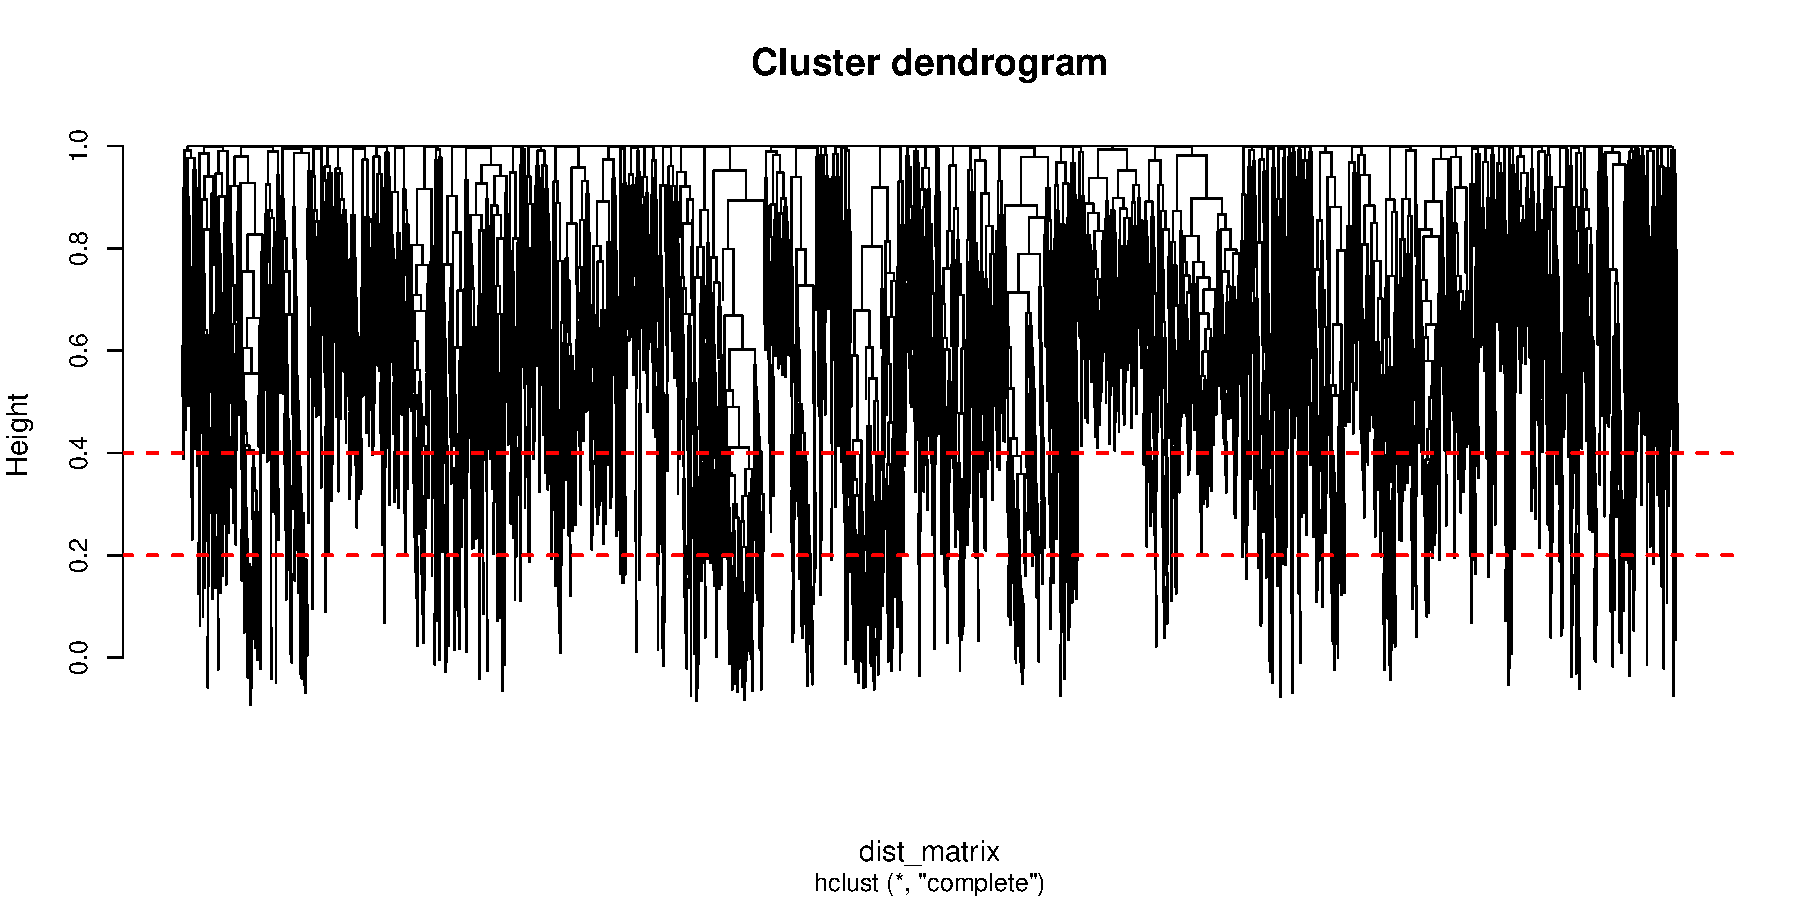
\includegraphics[width=0.95\linewidth]{figure/BMI_protein_INTERVAL/dendrogram} 

}

\caption[Cluster dendrogram showing the hierarchical relationship between protein levels]{\textbf{Cluster dendrogram showing the hierarchical relationship between protein levels.} Height is calculated as (1-correlation coefficient). At a height of 0.2 and 0.4 (red dashed lines), the number of independent proteins was 3,655 and 3,016 respectively}\label{fig:Dend-proteins}
\end{figure}
\elandscape

The association between BMI and specific platelet proteins were also explored. Here, GO pathways which include the term ``platelet'' were selected in AmiGO2 \url{http://amigo.geneontology.org/} (Supplementary Table 1). These pathways were then searched in BioMart \url{https://www.ensembl.org/biomart/martview/afd335dff2c91c86501d3f1f77b8b805}, to provide a list of all the proteins involved in these platelet pathways (Supplementary Table 2). Unique proteins in Supplementary Table 2 were searched within the results to extract the estimate for BMI on platelet proteins. As the chemokines MDC and TARC were explored in the previous chapter, the specific effects of BMI on MDC and TARC were looked up.

\hypertarget{enrichment-analysis}{%
\subsection{Enrichment analysis}\label{enrichment-analysis}}

To investigate whether any protein groups showed a particularly strong relationship with BMI and disease (signal detection), protein features were clustered for further analysis. First, a principal component analysis (PCA; prcomp() function from the R ``stats'' package) on the proteins, not the individuals, was performed on the ``pre-adjusted'' (see above) dataset (Figure \ref{fig:PCs}A-D). The top ``n'' PC eigenvectors, as identified by a scree plot of the PCA eigenvalues (Figure \ref{fig:PCs}E), were carried forward into an unsupervised k-means analysis (kmeans() function from the R ``stats'' package). Nineteen k-means analyses were run altering the value of k (number of clusters) from two to 20. To identify an appropriate number of protein clusters (k) a scree like plot was generated (Figure \ref{fig:PCs}F). Here the variance explained by clusters was plotted, for each k, as estimated as the sum of squares explained by clusters (betweenness) over the total sums of squares, and looked for the smallest k with the maximum variance explained (a plateau). In summary, a data reduction method (PCA) was used to identify major axes (PCs) of the protein data that were then utilised in a machine learning clustering algorithm (k-means) to identify clusters of proteins that share abundance similarities across individuals.



\begin{figure}

{\centering 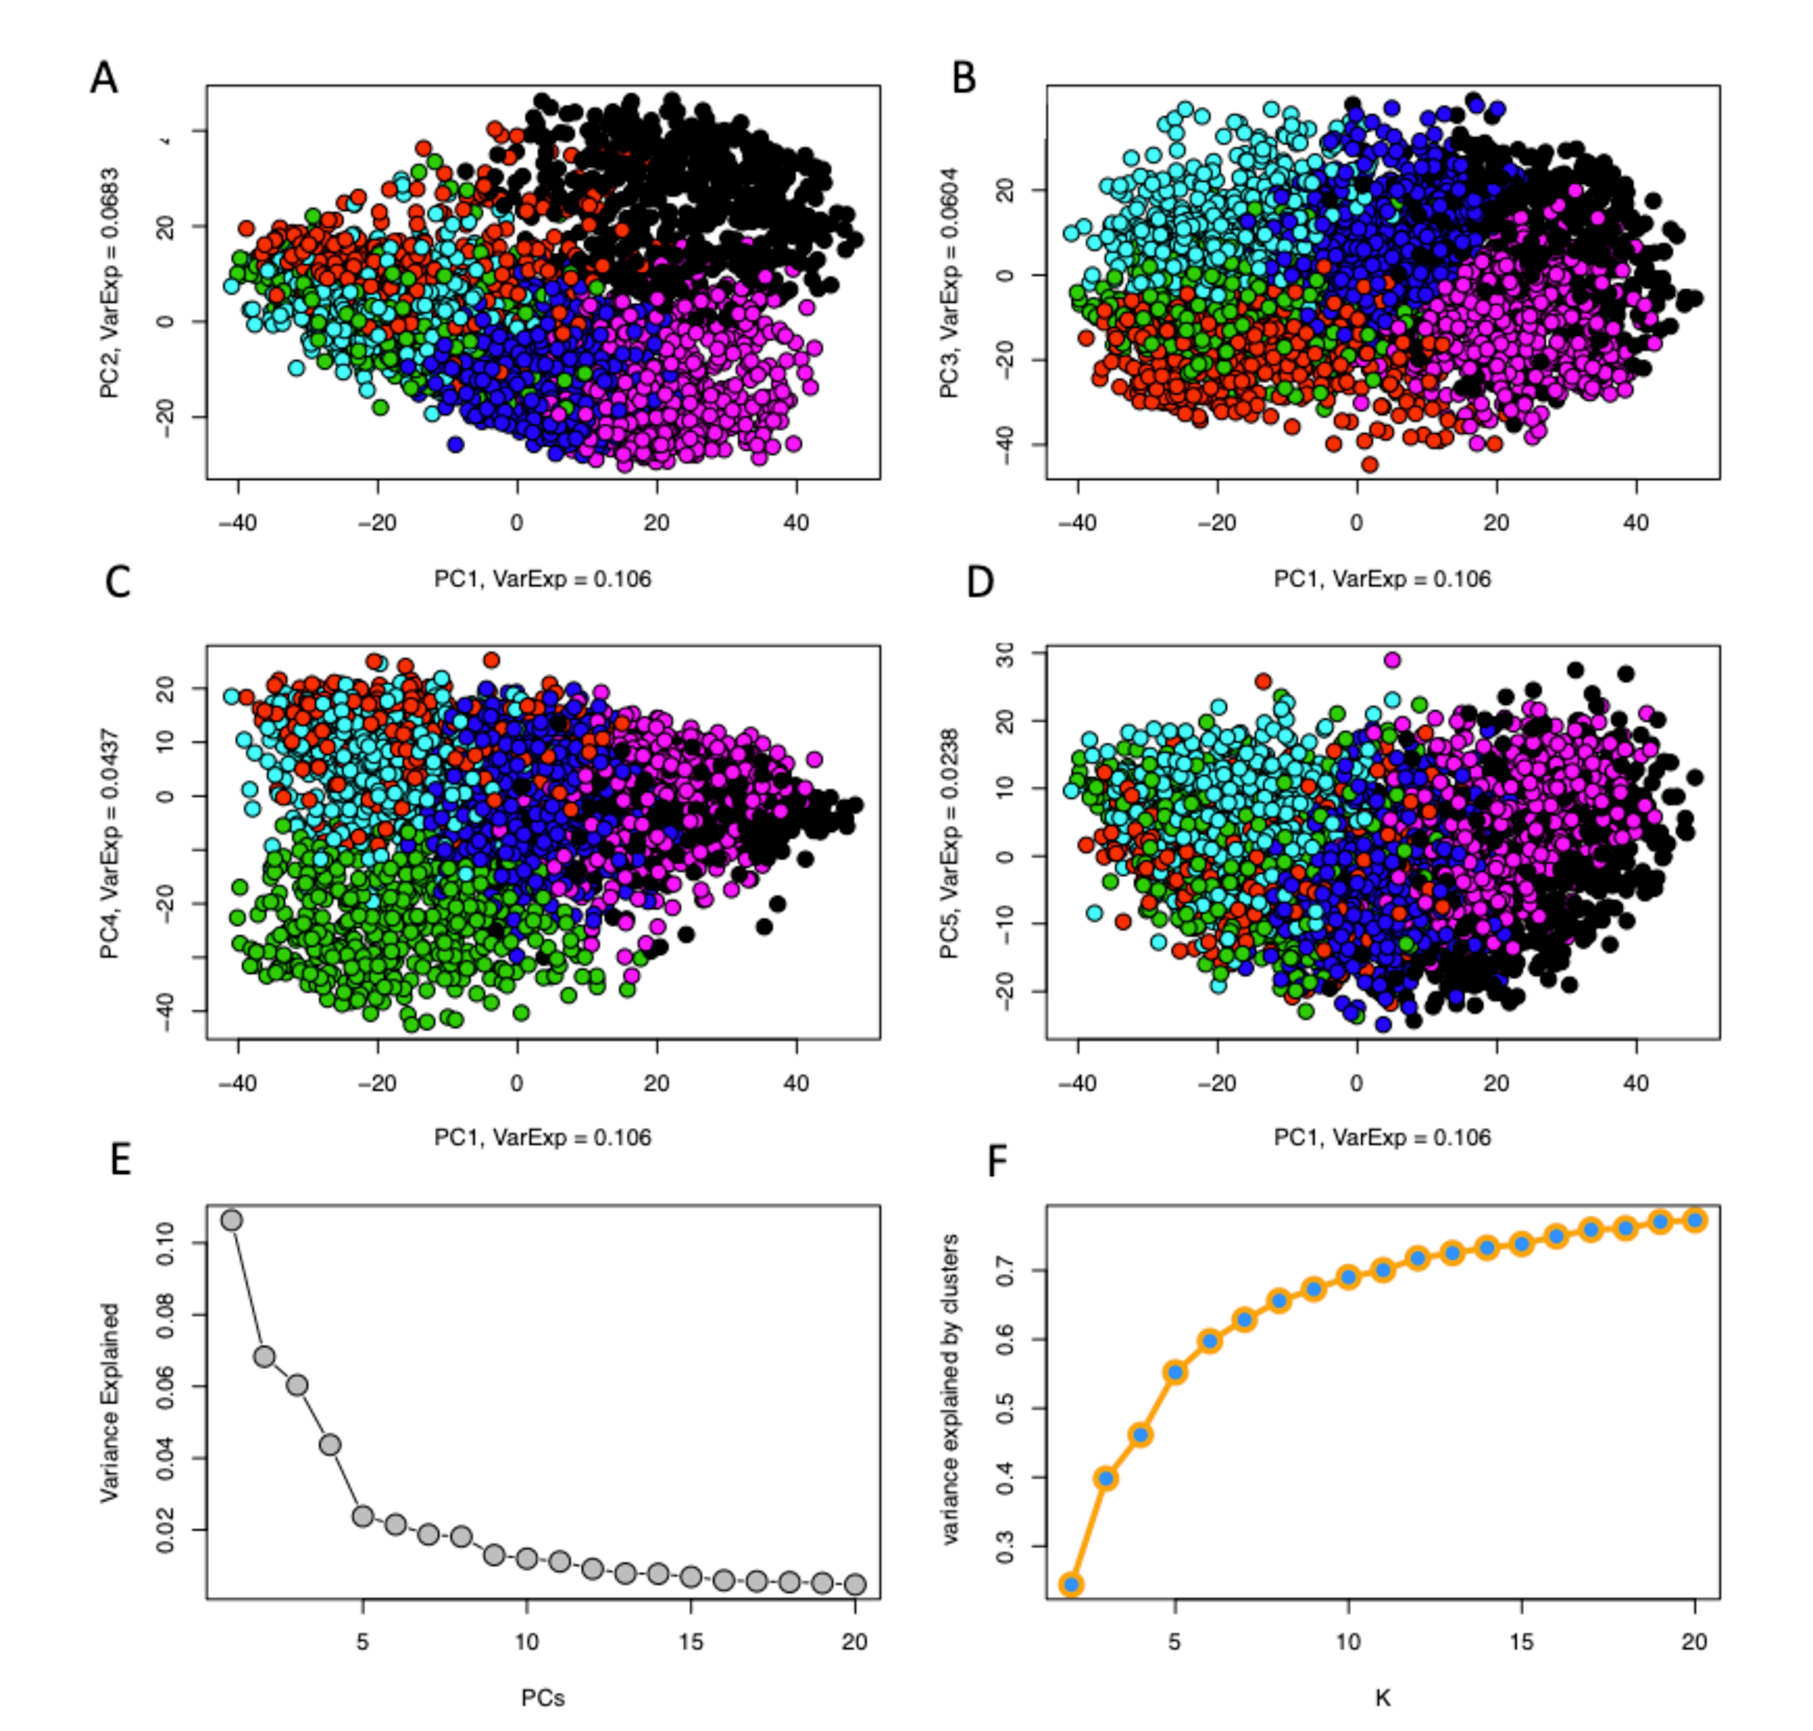
\includegraphics[width=0.9\linewidth]{figure/BMI_protein_INTERVAL/PCs2to5v1} 

}

\caption[Principal component analysis (PCA) and k-means clustering of proteins]{\textbf{Principal component analysis (PCA) and k-means clustering of proteins.} Principal component analysis (PCA) and k-means clustering of proteins provide evidence for five clusters. A-D) Principal component (PC) 1 vs PC2-PC5 for the study protein data. Each dot represents a protein, and the colors represent the clusters identified by the k-means analysis (1=black, 2=red, 3=green, 4=dark blue, 5=light blue, 6=pink). E) PC scree plot displaying the proportion of variance explained by each of the first 20 PCs. F) K-means scree like plot displaying the variance explained by clusters for each of the 19 k-means analysis, where in each analysis k (the number of clusters) was set from two to 20.}\label{fig:PCs}
\end{figure}
To explore whether there was a systematic difference in the association of proteins within these clusters and BMI, the beta coefficients from the observational linear regressions or MR models were transformed into their absolute values and divided by their standard error (SE). The absolute betas divided by their SEs in each cluster was compared using a one-tailed pairwise Wilcox test to identify which clusters showed a stronger association with BMI. For the cluster(s) showing evidence for larger absolute beta coefficients, an enrichment analysis was performed using DAVID bioinformatics resources 6.8\textsuperscript{\protect\hyperlink{ref-Huang2009}{157}}. Enrichment was assessed by using the uniprot IDs for the proteins in the cluster and comparing these proteins with the uniprot IDs of the full SomaLogic protein list. Enrichment for protein involvement in disease (using the genetic association database (GAD) disease classes\textsuperscript{\protect\hyperlink{ref-Becker2004a}{158}}) of the protein cluster was assessed by fold enrichment and a Bonferroni-corrected P-value to account for multiple testing. Disease classes are broadly grouped, therefore the main disease class of interest is cardiovascular disease as this class would incorporate CHD/stroke. Proteins that were associated with BMI in confounder-adjusted observational analyses at P\textless1.4x10\textsuperscript{-5} were also entered into the disease enrichment tool and compared with the total proteins (as described for cluster enrichment). Analyses were performed using R version 3.4.2\textsuperscript{\protect\hyperlink{ref-Team2019a}{109}}.

\hypertarget{results-3}{%
\section{Results}\label{results-3}}

\hypertarget{participant-characteristics-1}{%
\subsection{Participant characteristics}\label{participant-characteristics-1}}

INTERVAL participants included in this study (those with proteomic data), had a mean age of 45.0 years (SD of 14.1 years) and 48.3\% were female (Table \ref{tab:Inc-excl-part}). Mean BMI was 25.9 kg/m\textsuperscript{2} (SD of 4.8 kg/m\textsuperscript{2}) and the majority of participants were non-smokers (59.1\%). Nearly a quarter (23.5\%) reported currently or previously smoking daily and 71.5\% reported drinking alcohol at least once a week. Participants with proteomic data were representative of the full INTERVAL cohort (Table \ref{tab:Inc-excl-part}).



\begin{landscape}\begin{table}

\caption[Comparison of included vs excluded INTERVAL participants for the BMI-proteome analysis]{\label{tab:Inc-excl-part}\textbf{Comparison of included vs excluded INTERVAL participants for the BMI-proteome analysis}}
\centering
\begin{tabu} to \linewidth {>{\raggedright\arraybackslash}p{6cm}>{\raggedright}X>{\raggedright}X>{\raggedright}X>{\raggedright}X>{\raggedright}X}
\toprule
Variable & Included Mean (SD) or \% & Included N & Excluded Mean (SD) or \% & Excluded N & P value for difference (Two tailed t-test or Chi2 test)\\
\midrule
Age & 45.0 (14.1) & 2737 & 44.9 (14.2) & 30721 & 0.76\\
Sex &  & 2737 &  & 30721 & 0.04\\
\hspace{1em}Male & 51.70\% &  & 49.70\% &  & \\
\hspace{1em}Female & 48.30\% &  & 50.30\% &  & \\
Weight (kg) & 78.5 (16.1) & 2736 & 78.6 (16.0) & 30719 & 0.26\\
\addlinespace
Height (cm) & 172.7 (9.7) & 2730 & 172.2 (9.6) & 30661 & 0.005\\
Body mass index (kg/m2) & 25.9 (4.8) & 2729 & 26.4 (4.7) & 30659 & 0.66\\
Smoking frequency &  & 2675 &  & 29958 & 0.88\\
\hspace{1em}Never & 59.10\% &  & 59.40\% &  & \\
\hspace{1em}Occasional & 11.90\% &  & 12.00\% &  & \\
\addlinespace
\hspace{1em}Most days or every day & 29.00\% &  & 28.50\% &  & \\
Alcohol intake frequency &  & 2422 &  & 27124 & 0.34\\
\hspace{1em}Rarely & 11.70\% &  & 12.60\% &  & \\
\hspace{1em}Less than once a week & 16.90\% &  & 17.10\% &  & \\
\hspace{1em}One or two times a week & 37.40\% &  & 37.70\% &  & \\
\addlinespace
\hspace{1em}Three to five times a week / most days & 34.10\% &  & 32.50\% &  & \\
\bottomrule
\end{tabu}
\end{table}
\end{landscape}
\hypertarget{observational-estimates-of-associations-of-bmi-with-protein-traits}{%
\subsection{Observational estimates of associations of BMI with protein traits}\label{observational-estimates-of-associations-of-bmi-with-protein-traits}}

In a linear regression model adjusted for age and sex among 2729 adults, BMI (per SD higher) was associated with 1576 proteins (39\%) at the level P \textless{} 1.4 x 10\textsuperscript{-5} (multiple testing reference point, Supplementary Table 3). In a second model additionally adjusting for frequencies of smoking and alcohol intake among 2380 adults, there were 1447 associations at the same reference point (Supplementary Table 4). The strongest positive associations were with leptin (0.74 SD, 95\% CI 0.71-0.77, P=9.9x10\textsuperscript{-324}) and adipocyte fatty acid binding protein (FABP4) (0.58 SD, 95\% CI 0.55-0.62, P=6.4x10\textsuperscript{-211}). BMI (per SD) was also strongly positively associated with inflammatory proteins such as Complement Factor I (0.46 SD, 95\% CI 0.43-0.50, P=5.6x10\textsuperscript{-122}) and CRP (0.44 SD, 95\% CI 0.41-0.48, P=8.2x10\textsuperscript{-112}). BMI (per SD) also showed strong negative associations with proteins such as insulin-like growth factor-binding protein (IGFBP) 2 (-0.48 SD, 95\% CI -0.51 to -0.44, P=2.7x10\textsuperscript{-133}) and sex hormone-binding globulin (SHBG) (-0.43 SD, 95\% CI -0.47 to -0.39, P=2.4x10\textsuperscript{-106}).

There were 262 unique platelet proteins that were analysed in INTERVAL, 121 were associated with BMI in the confounder adjusted model (46\%). There was evidence that proteins involved in platelet pathways were associated with BMI. Higher BMI was negatively associated with antithrombin-III (-0.26 SD, 95\% CI -0.30 to -0.22, p=9.6x10\textsuperscript{-42}). BMI was also negatively associated with platelet-activating factor acetylhydrolase (PAFAH) (-0.26 SD, 95\% CI -0.30 to -0.23, p=4.9x10\textsuperscript{-39}), as was platelet endothelial aggregation receptor 1 (PEAR1) (-0.20 SD, 95\% CI -0.24 to -0.16, p=1.24x10\textsuperscript{-23}). Other proteins that were negatively associated with BMI include platelet endothelial cell adhesion molecule (PECAM-1), platelet glycoprotein Ib alpha chain (GPIbα) and platelet-derived growth factor receptor beta (PDGF Rb) (Supplementary Table 4 \& Supplementary Table 5). BMI was positively associated with the chemokine MDC (0.18 SD, 95\% CI 0.14-0.22, p=3.6x10\textsuperscript{-21}), but was not associated with TARC (Supplementary Table 3).

\hypertarget{observational-associations-of-covariables-with-bmi-and-protein-traits}{%
\subsection{Observational associations of covariables with BMI and protein traits}\label{observational-associations-of-covariables-with-bmi-and-protein-traits}}

Age, sex, and frequencies of smoking and alcohol intake were each associated with BMI (Table \ref{tab:INT-confounders-BMI}). Males had a higher BMI than females (0.17 SD, 95\% CI 0.10-0.25, P=5.8x10\textsuperscript{-6}). Age was positively associated with BMI (0.01 SD higher per year older, 95\% CI 0.009-0.015, P=1.2x10\textsuperscript{-18}). Smoking frequency was positively associated with BMI, but alcohol intake frequency was negatively associated with BMI. Covariables (age, sex, smoking and alcohol) showed associations with protein traits (Supplementary Tables 6-9 and Figures \ref{fig:QQ-confounder-proteins} A-D). There was evidence for 18 associations between age and proteins, 26 associations between sex and proteins, 38 proteins associated with smoking and 137 proteins associated with alcohol at the Bonferroni-adjusted level of p\textless1.4x10\textsuperscript{-5}.



\begin{landscape}\begin{table}

\caption[Associations between covariables (exposure) and standardised BMI (outcome)]{\label{tab:INT-confounders-BMI}\textbf{Associations between covariables (exposure) and standardised BMI (outcome)}}
\centering
\begin{tabu} to \linewidth {>{\raggedright\arraybackslash}p{4cm}>{\raggedright}X>{\raggedright\arraybackslash}p{2cm}>{\raggedright}X>{\raggedright}X>{\raggedright}X>{\raggedright}X>{\raggedright}X>{\raggedright}X>{\raggedright}X}
\toprule
Variable & N & Beta coefficient per 1-unit increase in confounder (SDs) & Standard error & P value & Adjusted R2 & F statistic & 95\% CI & Lower 95\% CI & Upper 95\% CI\\
\midrule
Age (years) & 2729 & 0.012 & 0.001 & 1.23e-18 & 0.028 & 78.8 & 0.003 & 0.009 & 0.015\\
Sex (1=female, 2=male) & 2729 & 0.17 & 0.038 & 5.8e-06 & 0.007 & 20.6 & 0.075 & 0.1 & 0.25\\
Smoking frequency (1=never, 2=occasinal, 3=most days/ every day) & 2667 & 0.022 & 0.022 & 3.16e-05 & 0.006 & 17.4 & 0.043 & 0.05 & 0.13\\
Alcohol intake frequency (1=rarely, 2=<1 a week, 3=1-2 times a week, 4=most days/every day) & 2415 & 0.021 & 0.021 & 7.08e-05 & 0.006 & 15.8 & 0.041 & -0.12 & -0.04\\
\bottomrule
\end{tabu}
\end{table}
\end{landscape}


\begin{figure}

{\centering 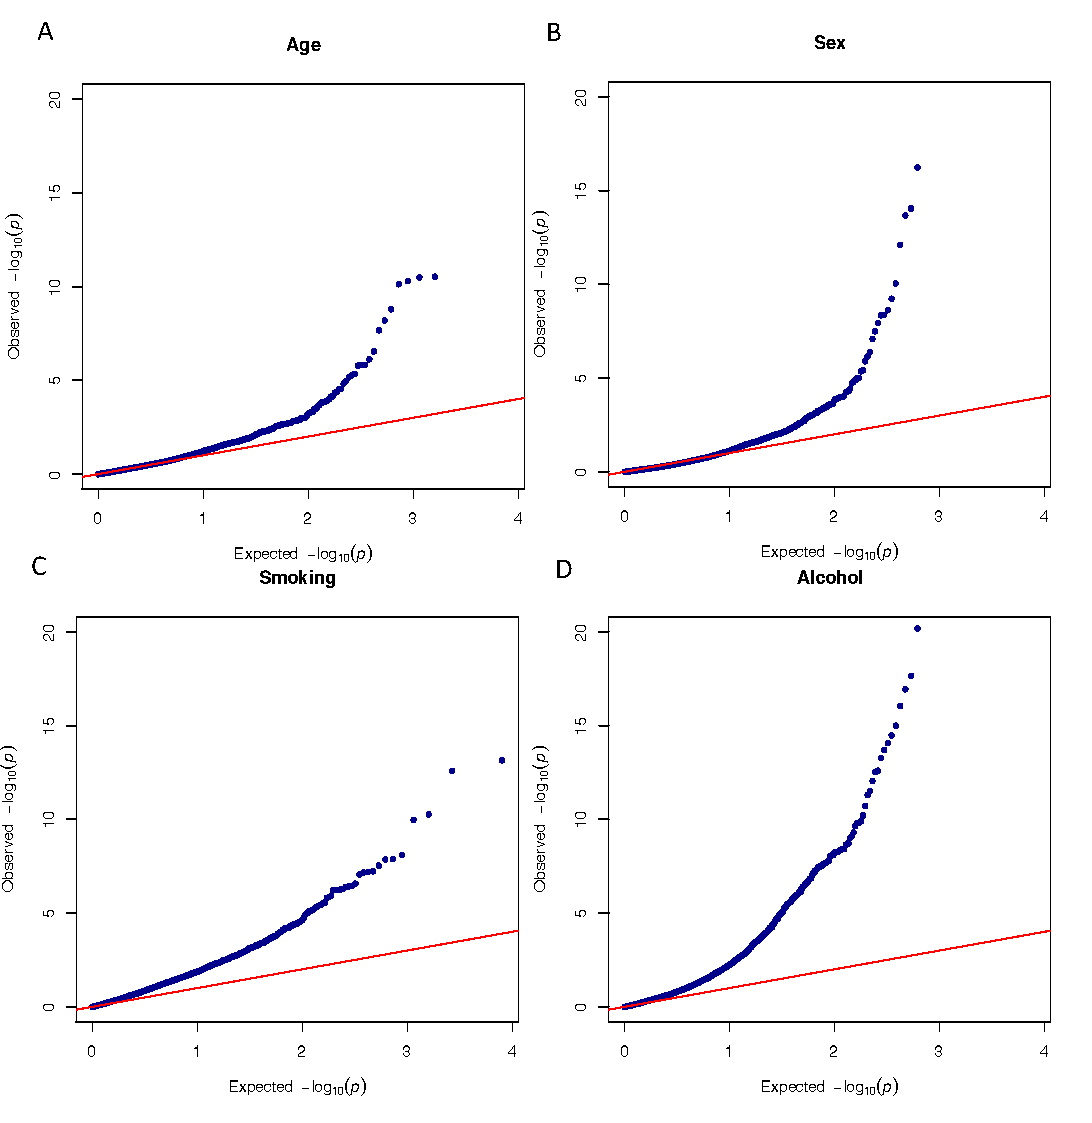
\includegraphics[width=0.95\linewidth]{figure/BMI_protein_INTERVAL/QQ_confounder_proteins} 

}

\caption[Q-Q plots of the expected against observed -log\textsubscript{10}(pvalues) for the associations between covariables and protein traits]{\textbf{Q-Q plots for the expected against observed -log\textsubscript{10}(pvalues) for associations of age (A), sex (B), smoking (C) and alcohol (D) with protein traits}. The red line indicates where the expected vs observed p-values are equal. Each blue dot represents the expected vs observed p-value for each protein.}\label{fig:QQ-confounder-proteins}
\end{figure}
\hypertarget{associations-of-the-grs-for-bmi-with-measured-bmi-and-covariables}{%
\subsection{Associations of the GRS for BMI with measured BMI and covariables}\label{associations-of-the-grs-for-bmi-with-measured-bmi-and-covariables}}

The distribution of the GRS among participants was normal (mean=0.08, SD=0.29, W=0.99, P=0.73, N=2729). The GRS was associated with BMI, explaining 2.8\% of its variance (R\textsuperscript{2}=0.028, P=1.6x10-18, Table \ref{tab:INT-GRS-confounders}). There was no strong evidence of association between GRS and age (R\textsuperscript{2}=0.001, P=0.11), sex (R\textsuperscript{2}=6x10-5, P=0.28), smoking frequency (R\textsuperscript{2}=\textless{} 0.0001, P=0.91), or alcohol intake (R\textsuperscript{2}\textless0.0001, P=0.44).



\begin{landscape}\begin{table}

\caption[Associations of the genetic risk score for BMI with reported BMI and covariables]{\label{tab:INT-GRS-confounders}\textbf{Associations of the genetic risk score for BMI with reported BMI and covariables}}
\centering
\begin{tabu} to \linewidth {>{\raggedright\arraybackslash}p{5cm}>{\raggedright}X>{\raggedright}X>{\raggedright}X>{\raggedright}X>{\raggedright}X>{\raggedright}X}
\toprule
Variable & N & Beta coefficient (per 1-unit increase in GRS) & Standard error & P value & Adjusted R2 & F statistic\\
\midrule
BMI (SDs) & 2729 & 0.57 & 0.06 & 1.64e-18 & 0.028 & 78.2\\
BMI (kg/m2) & 2729 & 2.54 & 0.31 & 4.82e-16 & 0.024 & 66.68\\
Age & 2737 & -1.47 & 0.92 & 0.11 & 0.001 & 2.55\\
Sex (1=female, 2=male) & 2737 & -0.04 & 0.03 & 0.28 & 5.96e-05 & 1.16\\
Smoking frequency (1=never, 2=occasinal, 3=most days/ every day) & 2675 & -0.02 & 0.14 & 0.91 & -4e-04 & 0.01\\
\addlinespace
Alcohol intake frequency (1=rarely, 2=<1 a week, 3=1-2 times a week, 4=most days/every day) & 2422 & -0.06 & 0.07 & 0.44 & -2e-04 & 0.6\\
\bottomrule
\end{tabu}
\end{table}
\end{landscape}
\hypertarget{mr-estimates-of-associations-between-bmi-and-protein-traits}{%
\subsection{MR estimates of associations between BMI and protein traits}\label{mr-estimates-of-associations-between-bmi-and-protein-traits}}

In MR analyses, eight unique BMI-protein associations were detected at the level P\textless1.4x10\textsuperscript{-5} (multiple testing reference point, Figure \ref{fig:ObsMRforestplot2}). MR estimates provide an estimate of the causal association between protein (in SDs) per SD higher BMI. The strongest association of BMI was again with leptin (0.63 SD, 95\% CI = 0.48-0.79; P=1.6x10\textsuperscript{-15}); this was followed by the association with FABP4 (0.65 SD, 95\% CI = 0.46-0.83; P=6.7x10\textsuperscript{-12}). A strong negative association was also seen between BMI (per SD) and SHBG (-0.45 SD, 95\% CI -0.65 to -0.25, P=1.4x10\textsuperscript{-5}). Other BMI-protein associations (P\textless1.4x10\textsuperscript{-5}) included positive associations with fumarylacetoacetase (FAAA), inhibin beta C chain and complement C5, and negative associations with receptor-type tyrosine-protein phosphatase delta and PILR alpha-associated neural protein.



\begin{figure}

{\centering 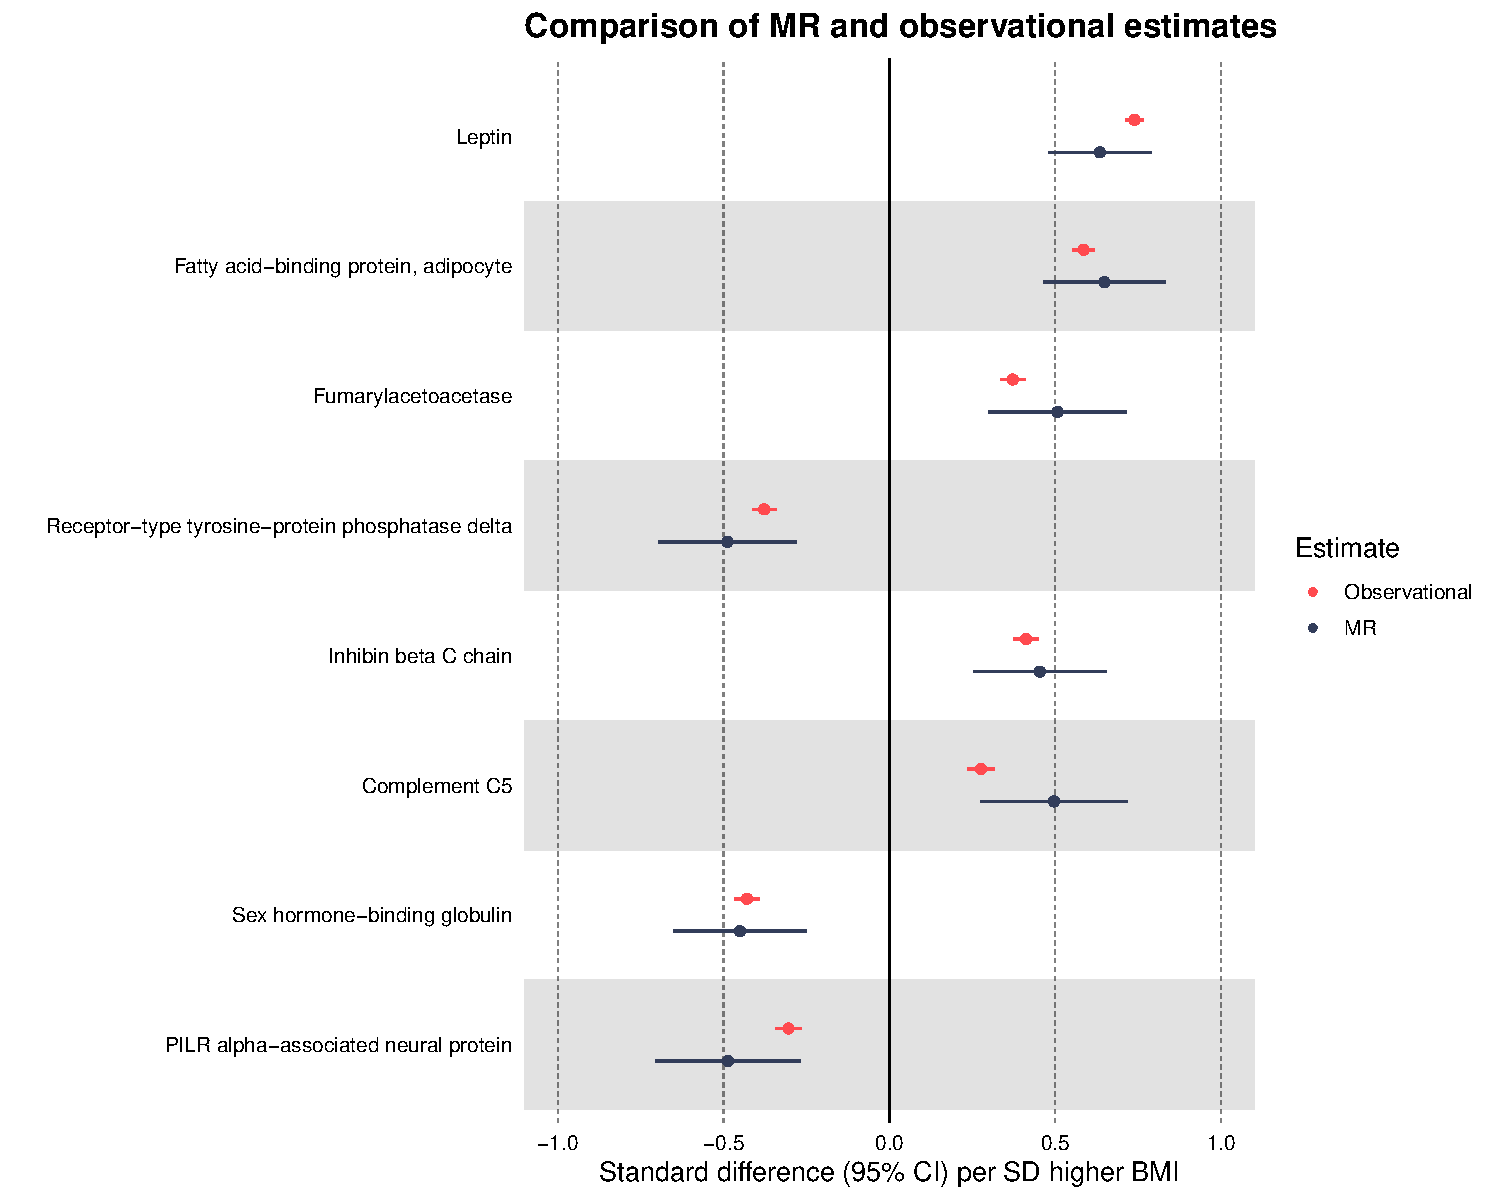
\includegraphics[width=0.9\linewidth]{figure/BMI_protein_INTERVAL/MR_obs_compar_forestplot} 

}

\caption[Forest plot of the strongest BMI-protein Mendelian randomisation estimates and the corresponding observational estimates]{\textbf{Forest plot of the strongest BMI-protein Mendelian randomisation estimates and the corresponding observational estimates}}\label{fig:ObsMRforestplot2}
\end{figure}
The estimates for the effect of BMI on platelet specific proteins did not pass multiple testing adjustment. Despite this, the MR estimates for the effect of BMI on platelet proteins generally were of a similar magnitude to the fully adjusted observational analysis, however none of the platelet proteins passed the multiple testing adjusted p-value. The causal estimate for the effects of BMI on PAFAH was -0.24 SD (95\% CI -0.46 to -0.03, p=0.028). Similarly, the causal estimate for the effect of BMI on PEAR1 was similar to the observational estimate (-0.21 SD, 95\% CI -0.43 to 0.005, p=0.06). Despite a similar magnitude of estimate, these associations were not detected as these estimates were less precise. Supplementary Table 10 provides the full MR results and Supplementary Table 5 has the observational and MR estimate for each platelet protein combined. The MR estimate for the effect of BMI on MDC was similar in magnitude (0.20 SDs, 95\% CI -0.02 to 0.42, p=0.069), but was less precise than the observational estimate, whereas there was no evidence for an effect on TARC (Figure \ref{fig:ObsMRforestplot-MDC-TARC}).



\begin{figure}

{\centering \includegraphics[width=0.9\linewidth]{figure/BMI_protein_INTERVAL/BMI_MDC_TARC_forestplot} 

}

\caption[Forest plot of the strongest BMI-protein Mendelian randomisation estimates and the corresponding observational estimates]{\textbf{Forest plot of the Mendelian randomisation estimates and the corresponding observational estimates for MDC and TARC}. Filled estimates indicate p\textless1.4x10\textsuperscript{-5}.}\label{fig:ObsMRforestplot-MDC-TARC}
\end{figure}
\hypertarget{comparison-of-observational-and-mr-estimates}{%
\subsection{Comparison of observational and MR estimates}\label{comparison-of-observational-and-mr-estimates}}

The distribution of P-values for associations between BMI and protein traits suggested an overrepresentation of signal for the observational estimates of BMI and protein traits; far more than expected from chance alone (Figure \ref{fig:QQ-obs-MR}A). In contrast to this, the extent of this overrepresentation was reduced considerably in the MR (Figure \ref{fig:QQ-obs-MR}B).



\begin{figure}

{\centering 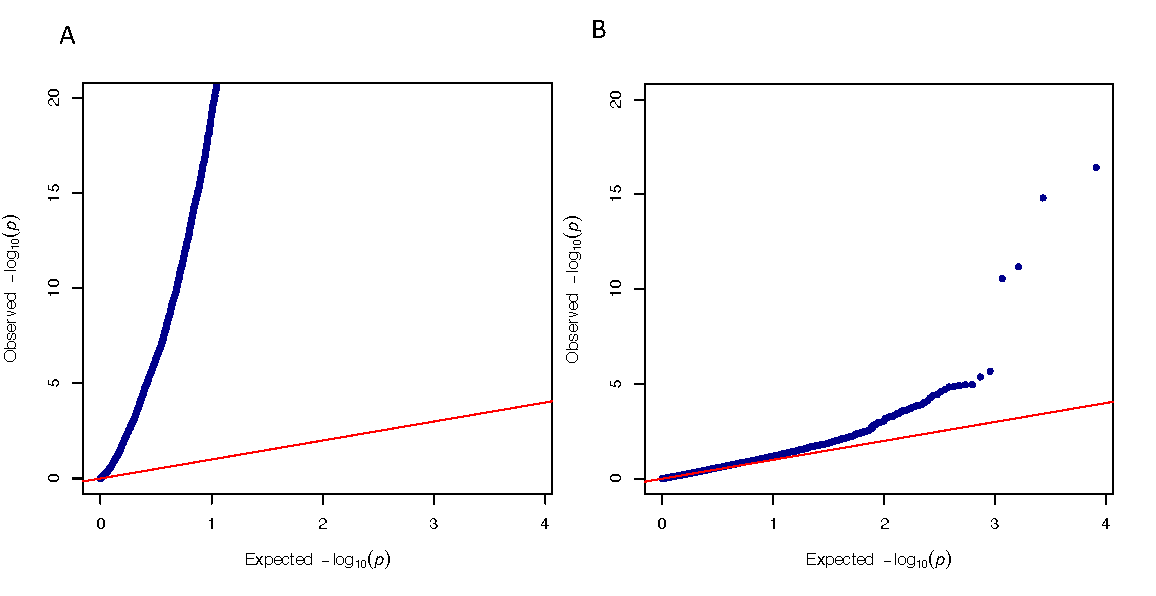
\includegraphics[width=0.95\linewidth]{figure/BMI_protein_INTERVAL/QQ_obs_MR} 

}

\caption[Q-Q plot of the expected against observed -log\textsubscript{10}(pvalues) for BMI-protein estimates]{\textbf{Q-Q plot of the expected against observed -log\textsubscript{10}(pvalues) for BMI-protein estimates.} A) Q-Q plot of expected against observed -log10(pvalues) for the unadjusted observational BMI-protein trait estimates B) Q-Q plot of expected against observed -log10(p) values for the Mendelian Randomization BMI-protein trait estimates.}\label{fig:QQ-obs-MR}
\end{figure}
The unadjusted and confounder-adjusted regression coefficients for BMI and protein traits were strongly associated (Beta=0.99 SDs, R\textsuperscript{2}=0.99, P=9.9x10\textsuperscript{-324}, Figure \ref{fig:Estimate-comparison-obs}). Compared with the observational estimates, the MR estimates were less precise, but there was a strong positive association between the beta coefficients from observational and MR estimates (Beta=0.68 SDs, R\textsuperscript{2}=0.33, P=9.9x10\textsuperscript{-324}) (Figure \ref{fig:Estimate-comparison-obs-mr}). After removing the proteins where P\textless1.4x10\textsuperscript{-5}, the strength of association between unadjusted and adjusted observational estimates remained, but the association between observational and MR estimates attenuated slightly (Figures \ref{fig:Obs-MR-without-top8} A/B). These results suggest causal effects of BMI across the general proteome.



\begin{figure}

{\centering 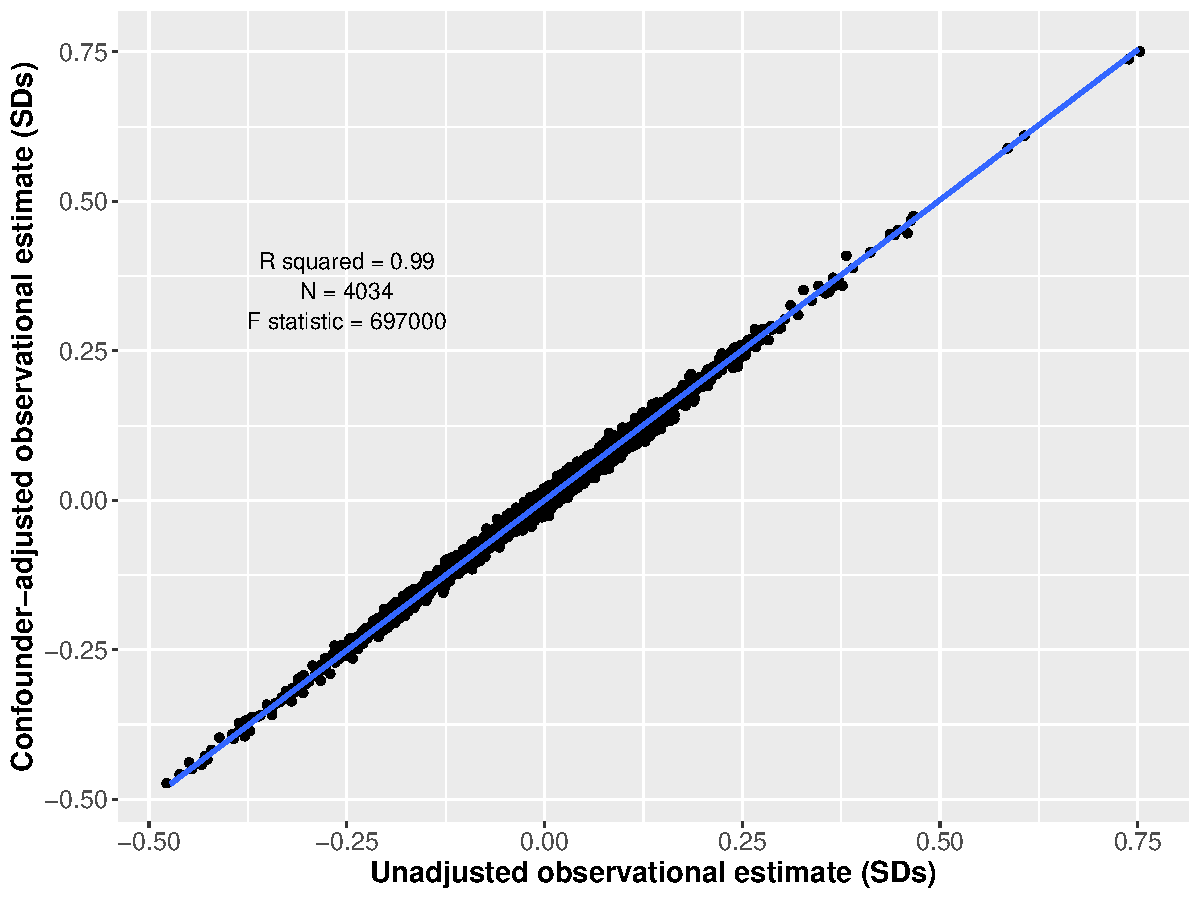
\includegraphics[width=0.65\linewidth]{figure/BMI_protein_INTERVAL/obs_v_obs_adj_scatter} 

}

\caption[Scatter plot comparing the unadjusted and confounder-adjusted observational BMI-protein estimates]{\textbf{Scatter plot of the unadjusted (age and sex adjusted) observational estimates and the confounder-adjusted observational estimates for BMI and protein traits}. Regression line shown in blue.}\label{fig:Estimate-comparison-obs}
\end{figure}


\begin{figure}

{\centering 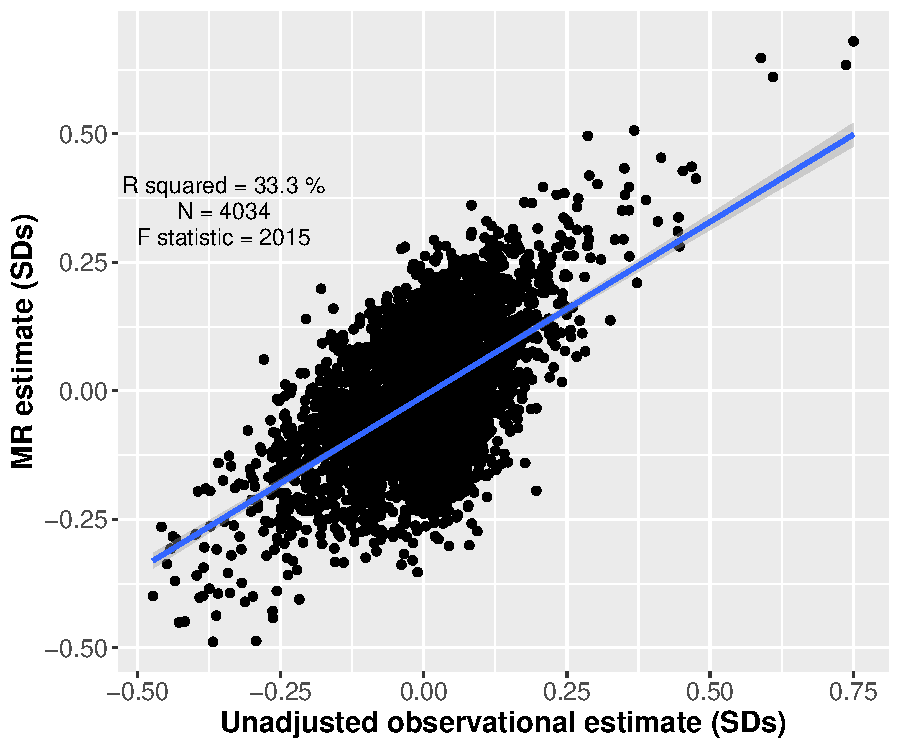
\includegraphics[width=0.65\linewidth]{figure/BMI_protein_INTERVAL/unadj_obs_MR_scatter_small} 

}

\caption[Scatter plot comparing the observational and MR BMI-protein estimates]{\textbf{Scatter plot of the unadjusted (age and sex adjusted) observational estimates and the MR estimates for BMI and protein traits.} Regression line shown in blue.}\label{fig:Estimate-comparison-obs-mr}
\end{figure}


\begin{figure}

{\centering 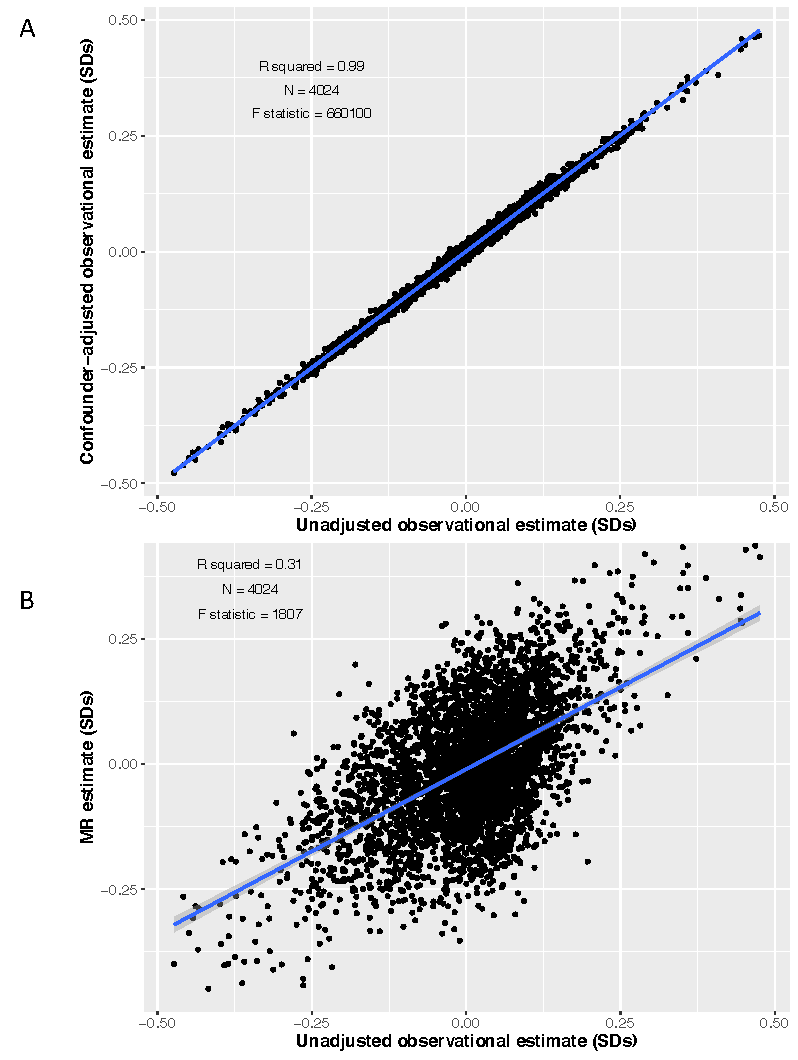
\includegraphics[width=0.8\linewidth]{figure/BMI_protein_INTERVAL/Obs_MR_scatter_without_top8} 

}

\caption[Scatter plot comparing BMI-protein estimates across models with top eight BMI-associated proteins excluded]{\textbf{Scatter plot comparing BMI-protein estimates across models with top eight BMI-associated proteins excluded.} A) Scatter plot of the unadjusted (age and sex adjusted) observational estimates and the confounder-adjusted observational estimates for BMI and protein traits with a regression line (blue) 6B) Scatter plot of the unadjusted (age and sex adjusted) observational estimates and the MR estimates for BMI and protein traits with a regression line (blue).}\label{fig:Obs-MR-without-top8}
\end{figure}
\hypertarget{enrichment-analysis-of-strongest-bmi-protein-associations}{%
\subsection{Enrichment analysis of strongest BMI-protein associations}\label{enrichment-analysis-of-strongest-bmi-protein-associations}}

In examining the clustering of proteins, visual representation using a scree plot suggested there were five PCs that explained 30.3\% of the variance (Figure \ref{fig:PCs}). After PC5 there was clear drop in variance explained, therefore other PCs were excluded. These five PCs were entered into a k-means analysis, which provided evidence for five clusters (grouping of individual proteins is included in Supplementary Table 10). To identify which cluster was most strongly affected by BMI, the median absolute beta coefficient divided by the SE for each cluster was compared with the overall estimate. Six of the proteins out of the eight strongest BMI-protein MR estimates were in cluster 2 (Supplementary Table 10). There was consistent evidence that cluster 2 showed a stronger association with BMI than the overall average BMI-protein effect both observationally (3.79 (IQR 1.62-7.06) vs 3.35 (IQR 1.57-5.83) respectively, P=3.7x10\textsuperscript{-4}) and in MR (0.85 (IQR 0.41-1.46) vs 0.74 (IQR 0.32-1.14), P=5.3x10\textsuperscript{-6}, Table \ref{tab:Cluster-estimates}). Cluster 2 showed consistent evidence of a having the largest BMI effect. Compared with the full protein list in SomaLogic, the proteins in cluster 2 were enriched for disease (Table \ref{tab:DAVID-enrichment-cluster2}), including cardiovascular disease (1.14 fold enrichment, P=1.3x10\textsuperscript{-4}), renal disease (1.22 fold enrichment, P=1.0x10\textsuperscript{-3}) cancer (1.1 fold enrichment, P=9.5x10\textsuperscript{-3}) and metabolic disease (1.08 fold enrichment, P=4.2x10\textsuperscript{-2}). No other individual cluster showed enrichment for disease. Enrichment for disease was also explored by comparing the proteins which had an association with BMI (P\textless1.4x10\textsuperscript{-5}) in the confounder-adjusted regression model with the total protein list. Compared with the full protein list, the proteins which showed a stronger observational association with BMI were enriched for renal disease (1.21 fold enrichment, P=0.001) and metabolic disease (1.9 fold enrichment, P=0.015, Table \ref{tab:DAVID-enrichment-obs}).



\begin{landscape}\begin{table}

\caption[Comparison of BMI-protein estimates among protein clusters]{\label{tab:Cluster-estimates}\textbf{Comparison of cluster median(absolute beta coefficient / SE) with the overall median for observational and MR analyses}. *One-tailed pairwise Wilcox test}
\centering
\begin{tabu} to \linewidth {>{\raggedright}X>{\raggedright}X>{\raggedright\arraybackslash}p{3cm}>{\raggedright}X>{\raggedright\arraybackslash}p{3cm}>{\raggedright}X}
\toprule
Cluster & N & Median absolute observational beta coefficient divided by SE (IQR) & P value* for cluster v all proteins (Observational) & Median MR beta coefficient divided by SE (IQR) & P value* for cluster v all proteins (MR)\\
\midrule
1 & 1061 & 3.28 (1.56-5.26) & 1 & 0.69 (0.31-1.22) & 1\\
2 & 1406 & 3.79 (1.62-7.06) & 3.70E-4 & 0.85 (0.41-1.46) & 5.3E-6\\
3 & 581 & 2.77 (1.39-4.30) & 1 & 0.74 (0.37-1.25) & 1\\
4 & 502 & 3.01 (1.25-5.6) & 1 & 0.68 (0.34-1.19) & 1\\
5 & 484 & 4.44 (2.2-7.05) & 1.80E-5 & 0.63 (0.32-1.14) & 1\\
\addlinespace
All & 4034 & 3.35 (1.57-5.83) &  & 0.74 (0.35-1.28) & \\
\bottomrule
\end{tabu}
\end{table}
\end{landscape}


\begin{landscape}\begin{table}

\caption[Cluster 2 vs full SomaLogic protein enrichment results for disease class using DAVID bioinformatics 6.8]{\label{tab:DAVID-enrichment-cluster2}\textbf{Cluster 2 vs full SomaLogic protein enrichment results for disease class using DAVID bioinformatics 6.8\textsuperscript{\protect\hyperlink{ref-Huang2009}{157}}}}
\centering
\begin{tabu} to \linewidth {>{\raggedright\arraybackslash}p{5cm}>{\raggedright}X>{\raggedright}X>{\raggedright}X>{\raggedright}X>{\raggedright}X>{\raggedright}X>{\raggedright}X>{\raggedright}X}
\toprule
Term (Genetic Association Database disease class) & Count & \% & List Total &   Population Hits & Population Total & Fold Enrichment & P Value & Bonferroni-adjusted P value\\
\midrule
Cardiovascular & 439 & 34.1 & 1024 & 1023 & 2723 & 1.14 & 7.3E-06 & 1.3E-04\\
Renal & 216 & 16.8 & 1024 & 472 & 2723 & 1.22 & 5.8E-05 & 1.0E-03\\
Cancer & 401 & 31.2 & 1024 & 958 & 2723 & 1.11 & 5.3E-04 & 9.5E-03\\
Pharmacogenomic & 357 & 27.8 & 1024 & 856 & 2723 & 1.11 & 1.9E-03 & 3.4E-02\\
Metabolic & 504 & 39.2 & 1024 & 1243 & 2723 & 1.08 & 2.4E-03 & 4.2E-02\\
\addlinespace
Vision & 100 & 7.8 & 1024 & 216 & 2723 & 1.23 & 5.9E-03 & 1.0E-01\\
Haematological & 168 & 13.1 & 1024 & 388 & 2723 & 1.15 & 9.8E-03 & 1.6E-01\\
Reproduction & 152 & 11.8 & 1024 & 351 & 2723 & 1.15 & 1.4E-02 & 2.3E-01\\
Immune & 360 & 28 & 1024 & 886 & 2723 & 1.08 & 1.5E-02 & 2.4E-01\\
Neurological & 311 & 24.2 & 1024 & 759 & 2723 & 1.09 & 1.6E-02 & 2.5E-01\\
\addlinespace
Aging & 117 & 9.1 & 1024 & 278 & 2723 & 1.12 & 7.5E-02 & 7.5E-01\\
\bottomrule
\end{tabu}
\end{table}
\end{landscape}


\begin{landscape}\begin{table}

\caption[Disease enrichment of proteins associated with BMI in confounder adjusted model compared with all proteins in SomaLogic (DAVID Bioinformatics 6.8)]{\label{tab:DAVID-enrichment-obs}\textbf{Disease enrichment of proteins associated with BMI in confounder adjusted model compared with all proteins in SomaLogic (DAVID Bioinformatics 6.8)\textsuperscript{\protect\hyperlink{ref-Huang2009}{157}}}}
\centering
\begin{tabu} to \linewidth {>{\raggedright\arraybackslash}p{5cm}>{\raggedright}X>{\raggedright}X>{\raggedright}X>{\raggedright}X>{\raggedright}X>{\raggedright}X>{\raggedright}X>{\raggedright}X}
\toprule
Term (Genetic Association Database disease class) & Count & \% & List Total &   Population Hits & Population Total & Fold Enrichment & P Value & Bonferroni-adjusted P value\\
\midrule
Renal & 218 & 16.4 & 1039 & 472 & 2723 & 1.21 & 7.7E-05 & 0.001\\
Pharmacogenomic & 372 & 28 & 1039 & 856 & 2723 & 1.14 & 8.8E-05 & 0.002\\
Metabolic & 515 & 38.8 & 1039 & 1243 & 2723 & 1.09 & 8.3E-04 & 0.015\\
Aging & 129 & 9.7 & 1039 & 278 & 2723 & 1.22 & 2.7E-03 & 0.047\\
Cardiovascular & 424 & 32 & 1039 & 1023 & 2723 & 1.09 & 4.1E-03 & 0.072\\
\addlinespace
Unknown & 233 & 17.6 & 1039 & 541 & 2723 & 1.13 & 6.4E-03 & 0.109\\
Psych & 228 & 17.2 & 1039 & 534 & 2723 & 1.12 & 1.2E-02 & 0.189\\
Reproduction & 154 & 11.6 & 1039 & 351 & 2723 & 1.15 & 1.4E-02 & 0.228\\
Normal variation & 86 & 6.5 & 1039 & 185 & 2723 & 1.22 & 1.5E-02 & 0.236\\
Other & 211 & 15.9 & 1039 & 497 & 2723 & 1.11 & 2.1E-02 & 0.313\\
\addlinespace
Cancer & 391 & 29.5 & 1039 & 958 & 2723 & 1.07 & 2.2E-02 & 0.332\\
Haematological & 164 & 12.4 & 1039 & 388 & 2723 & 1.11 & 5.0E-02 & 0.605\\
Neurological & 309 & 23.3 & 1039 & 759 & 2723 & 1.07 & 5.5E-02 & 0.638\\
Developmental & 160 & 12.1 & 1039 & 381 & 2723 & 1.1 & 6.6E-02 & 0.708\\
\bottomrule
\end{tabu}
\end{table}
\end{landscape}
\hypertarget{discussion-3}{%
\section{Discussion}\label{discussion-3}}

This chapter sought to estimate the effects of adiposity on a comprehensive set of protein traits only recently measurable by untargeted proteomics using observational and MR methods. This analysis was performed as alterations in the plasma proteins may have implications for cardiovascular disease, and therefore relating to platelet function. Observational results provided evidence for associations between BMI and 1576 proteins and MR was performed to reduce confounding. MR results suggest that BMI alters protein traits involved in regulating appetite, sex hormones, inflammation, and other systems; specific proteins most altered by BMI include leptin, FABP4, and SHBG. Results of follow-up analyses suggest that the cluster of proteins most altered by BMI is enriched for genes associated with cardiovascular and metabolic disease.

This chapter explored the effect of BMI on a large set of circulating proteins in an MR framework. Previous studies have used observational epidemiology to explore the effect of obesity on the plasma proteome: one study used mass spectrometry and found an increase in Complement Factors I, B and H and an increase in CRP\textsuperscript{\protect\hyperlink{ref-Cominetti2018}{93}}. These findings were replicated in our current observational analysis using the SomaLogic platform, indicating that associations are detectable across different proteomic platforms. The only association that did not replicate in the current analysis was the positive association with protein S100-A9. Although the MR analysis did not support some of these BMI-protein associations as being causal based on a P-value reference point, the strong association between the observational and MR estimates throughout the entire effect distribution suggests that disagreements between methods are likely an issue of power given current sample sizes.

Previous work implementing MR to examine the relationship between BMI and \textasciitilde1000 proteins (measured using the same SomaLogic array) provided corroborative evidence to that shown here\textsuperscript{\protect\hyperlink{ref-Zaghlool2021}{88}}. Both studies suggested a positive association between BMI and leptin, as well as a negative association with SHBG. Other proteins, such as IGFBP1/2 and growth hormone receptor, did not pass our multiple testing threshold, but the direction and magnitude of estimates were in agreement, suggesting a possible causal effect that was not detectable in the current analysis. Building on previous work, the current chapter provides MR estimates for \textgreater3600 proteins, offering a wider proteomic profile and detecting additional associations such as that between BMI and fumarylacetoacetase and inhibin beta C chain. Furthermore, the inclusion of over threefold more proteins allowed a more comprehensive enrichment analysis to be performed.

For proteins with stronger MR derived association evidence, it is important to explore whether they have a potential role in disease. Identification of individual proteins could help to guide future intervention if changes in proteins can be mapped to disease outcomes. Our results suggest a strong positive effect of BMI on levels of leptin, a hormone released by white adipose tissue which suppresses appetite\textsuperscript{\protect\hyperlink{ref-Klok2007}{159}}. The direction of effect agrees with estimates from previous cross-sectional and MR studies\textsuperscript{\protect\hyperlink{ref-Wurtz2014}{32},\protect\hyperlink{ref-Millard2015}{160}}, indicating leptin receptor resistance\textsuperscript{\protect\hyperlink{ref-Gruzdeva2019a}{161}}. There is observational evidence in humans that higher leptin can induce greater aggregation of platelets (cells involved in haemostasis)\textsuperscript{\protect\hyperlink{ref-Nakata1999}{162}}. In a larger observational study, leptin was found to be associated with higher risk of coronary events independent of BMI\textsuperscript{\protect\hyperlink{ref-Wallace2001}{163}}.

Our results help to provide contextualisation for proteins which have already been implicated in disease. For example, results suggest a strong positive effect of BMI on FABP4, an adipokine found primarily in adipocytes and macrophages\textsuperscript{\protect\hyperlink{ref-Furuhashi2014}{164}}. This MR estimate supports the association which has been suggested in previous observational studies\textsuperscript{\protect\hyperlink{ref-Xu2006}{165}}. FABP4 has been implicated in cardiometabolic disease: a SNP which increases FABP4 was found to raise the odds of type II diabetes among adults\textsuperscript{\protect\hyperlink{ref-Gudmundsdottir2020}{166}}, potentially through its contribution to higher insulin resistance\textsuperscript{\protect\hyperlink{ref-Nakamura2017}{167}}. FABP4 has also been associated with higher risk of atherosclerosis among adults\textsuperscript{\protect\hyperlink{ref-Yeung2007}{168}}. A strong SHBG-lowering effect of higher BMI was also suggested here. The SHBG molecule is a glycoprotein which binds androgens and oestrogens and suppresses their activity\textsuperscript{\protect\hyperlink{ref-Wallace2013}{169}}; a reduction in SHBG is therefore expected to lead to higher levels of circulating sex hormones. The negative effect of BMI on SHBG seen here supports observational findings\textsuperscript{\protect\hyperlink{ref-Cooper2015}{170}--\protect\hyperlink{ref-Baglietto2009}{172}}. When evaluating the role of SHBG in disease, MR analysis suggests that an increase in SHBG contributes to a decrease in risk of cardioembolic stroke\textsuperscript{\protect\hyperlink{ref-Zheng2020}{146}}. Other studies have also implicated lower SHBG levels in increasing type II diabetes risk.\textsuperscript{\protect\hyperlink{ref-Ritchie2019}{173}} The exact mechanisms leading from decreased SBHG to ill-health is unclear, but may arise as a result of the increased bioavailability of testosterone and oestrogen\textsuperscript{\protect\hyperlink{ref-Wallace2013}{169}}.

There were also a range of platelet proteins which were detected in the plasma (262 proteins). These are proteins which have been linked to platelet GO pathways. The observational analysis detected an inverse association between BMI and platelet proteins, including PAFAH and PEAR1. These estimates were similar in the MR analysis, however the estimates did not pass multiple testing adjustment. Interestingly, higher BMI led to a decrease in levels of these proteins circulating in the plasma. PAFAH is a phospholipase A\textsubscript{2} enzyme.\textsuperscript{\protect\hyperlink{ref-Marathe2018}{174}} PAFAH binds to lipoproteins and can degrade platelet activating factor (PAF). The degradation of PAF leads to a reduction in aggregation. PAFAH has been shown to bind to lipoproteins in mice\textsuperscript{\protect\hyperlink{ref-Noto2003}{175}} and is thought to therefore reduce lipoprotein oxidation, thereby being antiatherogenic. The reduction in PAFAH that was associated with higher BMI could therefore be atherogenic. It is unclear why higher BMI would lead to a reduction in other proteins such as PEAR1. PEAR1 is a transmembrane protein involved in megakaryopoiesis and platelet activation, where it plays a key role in stabilising integrin α\textsubscript{IIb}β\textsubscript{3}\textsuperscript{\protect\hyperlink{ref-Kauskot2012}{176}}. Lower circulating levels of PEAR1 in participants with higher BMI could be explained by PEAR1 levels being retained more within the platelet (and therefore could lead to platelet hyperactivity). Although alterations in plasma proteins may help understanding of the environment platelets are in, it would be informative to explore the platelet proteome in a cohort as large as INTERVAL, however the material is not available for this analysis.

The involvement of the chemokines MDC and TARC in platelet function was presented in Chapter \ref{chemokine-platelets}, where there was evidence that they can modulate platelet activation. There was also MR evidence that higher levels of MDC could contribute towards VTE pathophysiology. These chemokines were also included in the SomaLogic panel in the current chapter, therefore the effect of BMI on the circulating levels of these chemokines was explored. MDC was associated with BMI observationally, and the magnitude of effect was similar in the MR, however this estimate did not withstand multiple testing adjustment. It is possible that MDC could be an intermediate in between BMI and platelet function, however this analysis needs to be replicated in a larger cohort. There was no evidence to support TARC as an intermediate. Differences in regulation of MDC and TARC need to be further elucidated.

Despite these possible protein involvements in cardiometabolic disease and platelet function, it remains difficult to assess the contribution of individual proteins as they are not entirely independent and any pathological effects would likely be due to a global change in protein composition. There are not distinct groupings in the SomaLogic data as there often are with, for example, metabolomics data. Proteins grouped into clusters of similar features were examined, where the BMI-protein estimates of each cluster with overall estimates were compared and enrichment for genes related to disease were explored. The cluster most altered by BMI (cluster 2) included most of the eight proteins with the strongest BMI effects from MR analyses, as well as various complement factors, chemokines and coagulation factors. Therefore, it is very likely that this global change in proteins would activate platelets. This cluster was also found to be enriched for genes related to cardiovascular disease, renal and metabolic diseases, and cancer. Enrichment was similar when comparing the proteins that had an observational association with BMI with all proteins included, with enrichment appearing greatest for renal and metabolic disease. Together, this suggests that changes in proteins may mediate effects of obesity on cardiometabolic diseases; more focused investigations of these proteins are now needed, especially to assess their impact on platelet function.

This analysis has some limitations. The limitations that have arisen through use of the INTERVAL study have been discussed in section \ref{INTERVAL-limitations}. One of the limitations specific to the proteomic data in INTERVAL is that although it is one of largest existing cohorts to have untargeted proteomic data based on the SomaLogic platform, the sample size is still relatively modest and may have low power to detect some associations when using MR. Based on the detectable (P\textless1.4x10\textsuperscript{-5}) median absolute observational effect size (0.13 SDs), our analyses had 80\% power to detect MR effect sizes \textgreater= 0.33 SDs (alpha=0.05) for our sample size (N=2737)\textsuperscript{\protect\hyperlink{ref-Brion2013}{177}}. With greater statistical power, there would likely be more proteins detected with MR. This was reinforced by the strong agreement in the magnitude of effect estimates seen in observational and MR analyses which applied throughout the effect distribution. Additionally, the proteins examined are highly correlated and therefore changes in individual proteins may not fully be described. Evidence from case-control cohorts as well as functional and animal studies would help isolate individual proteins that are altered and contribute to disease. Finally, although analyses provide insight into the proteomic effects of BMI, it does not distinguish between the type of adiposity. It would be useful to distinguish between the effects of subcutaneous and visceral fat using dual-energy X-ray absorptiometry (DXA) derived measurements, but these were not available in the INTERVAL data set.

This chapter utilised SomaLogic to explore the relationship between BMI and plasma proteins in unprecedented scope and detail, in both an observational and MR framework. There is evidence for a broad impact of higher adiposity on the circulating proteome. Causal evidence was strongest for BMI in relation to proteins involved in regulating appetite, sex hormones, and inflammation. Protein alterations were found to be enriched for genes related to cardiovascular and metabolic disease, therefore implicating an environment which may lead to platelet hyperactivity. Altogether, these results help to focus attention onto new potential proteomic signatures of obesity-related disease. Further characterisation of the role of such proteomic profiles in cardiovascular disease using MR is warranted, as well as characterising the role of such proteins on platelet function.

\hypertarget{BMI-protein-RCT}{%
\chapter{Further elucidating the effect of adiposity on the plasma proteome using a weight loss intervention}\label{BMI-protein-RCT}}

\hypertarget{background-4}{%
\section{Background}\label{background-4}}

Obesity is associated with an increased risk of type II diabetes (T2D), cardiovascular diseases, musculoskeletal diseases, and types of cancer\textsuperscript{\protect\hyperlink{ref-Khan2018}{10},\protect\hyperlink{ref-Garg2014}{178},\protect\hyperlink{ref-Kortt2002}{179}}. These associations are well established, however mechanisms of disease are less clear. It is likely that a change in the composition of proteins circulating in the blood plays a role in obesity-related cardiovascular risk\textsuperscript{\protect\hyperlink{ref-Goudswaard2021}{154}}. The previous results chapter (Chapter \ref{BMI-protein-MR}) examined the effect of BMI on the plasma proteome and provided estimates for the average change in proteins per average difference in BMI in a general population, using observational estimates and one sample Mendelian randomization (MR). There was evidence of a BMI effect on proteins such as leptin, sex hormone binding globulin (SHBG), fatty acid binding protein 4 (FABP4) and fumarylacetoacetase. Within an enrichment analysis, this change in circulating levels of these proteins was implicated in cardiovascular diseases. There is also evidence that obesity affects platelet function, thereby elevating the risk of thrombotic events. There is evidence from the literature and from Chapter \ref{chemokine-platelets} that circulating proteins could mediate this risk.

Although MR helps to overcome issues inherent to observational studies such as confounding and reverse causation, MR has its own limitations. For example, it is possible that genetic variants used for the genetic risk score could affect protein levels through routes other than changes in BMI. This is known as horizonal pleiotropy\textsuperscript{\protect\hyperlink{ref-Davies2018}{12}}. As well as this, although there were over 2700 particpants within the MR, this is a relatively small sample size for the study design. Additionally, it is important to not only look at which proteins are altered within the population with higher BMI; identifying which proteins can be modulated with weight loss is important as this may help reveal mechanistic insight into mechanisms of obesity-related cardiovascular disease. Triangulation can therefore be used in efforts to further determine the BMI effects on the plasma proteome. Triangulation is defined as strengthening causal inference through the combination of study designs which each have separate sources of bias\textsuperscript{\protect\hyperlink{ref-Lawlor2016}{180}}. Therefore, to add an independent source of evidence to the MR in the previous chapter, the Diabetes REmission Clinical Trial (DiRECT) can be utilised. The DiRECT trial consisted of a group of patients with overweight/obesity and T2D who were either given guideline T2D care or an acute intervention, consisting of a low calorie diet, to help with weight loss and T2D remission\textsuperscript{\protect\hyperlink{ref-Lean2018}{181}}. This chapter therefore aims to: examine the effect of reducing BMI with caloric restriction on the plasma proteome.



\begin{figure}

{\centering \includegraphics[width=0.8\linewidth]{figure/DiRECT/Thesis_graphic_overview_BMI_protein_CVD} 

}

\caption[Schematic of the associations explored in Chapter \ref{BMI-protein-RCT}]{\textbf{Schematic of the associations explored in Chapter \ref{BMI-protein-RCT}. This chapter explores the effect of caloric restriction-induced weight loss on the plasma proteome.} Figure made using BioRender.com.}\label{fig:BMI-protein-graphic2}
\end{figure}
\hypertarget{methods-3}{%
\section{Methods}\label{methods-3}}

\hypertarget{study-design-and-participants}{%
\subsection{Study design and participants}\label{study-design-and-participants}}

Samples analysed within this study were collected from participants enrolled in the Diabetes Remission clinical trial (DiRECT). DiRECT was a cluster-randomised trial which took place at 49 primary care practices in Scotland and Tyneside\textsuperscript{\protect\hyperlink{ref-Lean2018}{181}}. Ethical approval was granted from West 3 Ethics Committee (January, 2014) and the National Health Service (NHS). Participants were recruited between 25th July 2014 and 5th August 2016. Details of the protocol have previously been published\textsuperscript{\protect\hyperlink{ref-Leslie2016}{182}}. Participants enrolled were between 20-65 years, diagnosed with T2D within previous 6 years, had a BMI of between 27-45kg/m\textsuperscript{2}. Participants were excluded if they were: using insulin, had a HbA1c concentration of ≥12 \% (≥108 mmol/mol), weight loss of \textgreater5 kg in the preceding 6 months, an estimated glomerular filtration rate of \textless30 mL/min per 1.732 m\textsuperscript{2}. Other exclusion criteria include heart failure, participation in other clinical trials, substance abuse, cancer, recent MI (\textless6 months), learning difficulties, current use of anti-obesity drugs, eating disorders, pregnancy or admission to hospital for depression or use of antipsychotic medication\textsuperscript{\protect\hyperlink{ref-Lean2018}{181}}. Participants in the control group received best-practice care by guidelines. The intervention group were asked to follow the Counterweight-Plus weight management programme\textsuperscript{\protect\hyperlink{ref-Lean2013}{183}}. This programme consisted of a total diet replacement (TDR) phase using a low energy diet (825-853 kcal/day) for 3-5 months, followed by structured food reintroduction of 2-8 weeks, with ongoing monthly long-term weight loss maintenance visits. Those in the intervention group had their antidiabetic and antihypertensive drugs discontinued. In total, there were 146 patients in the control group and 119 in the intervention group who remained enrolled in the study at 1 year, as detailed in Figure \ref{fig:direct-participants}.



\begin{figure}

{\centering 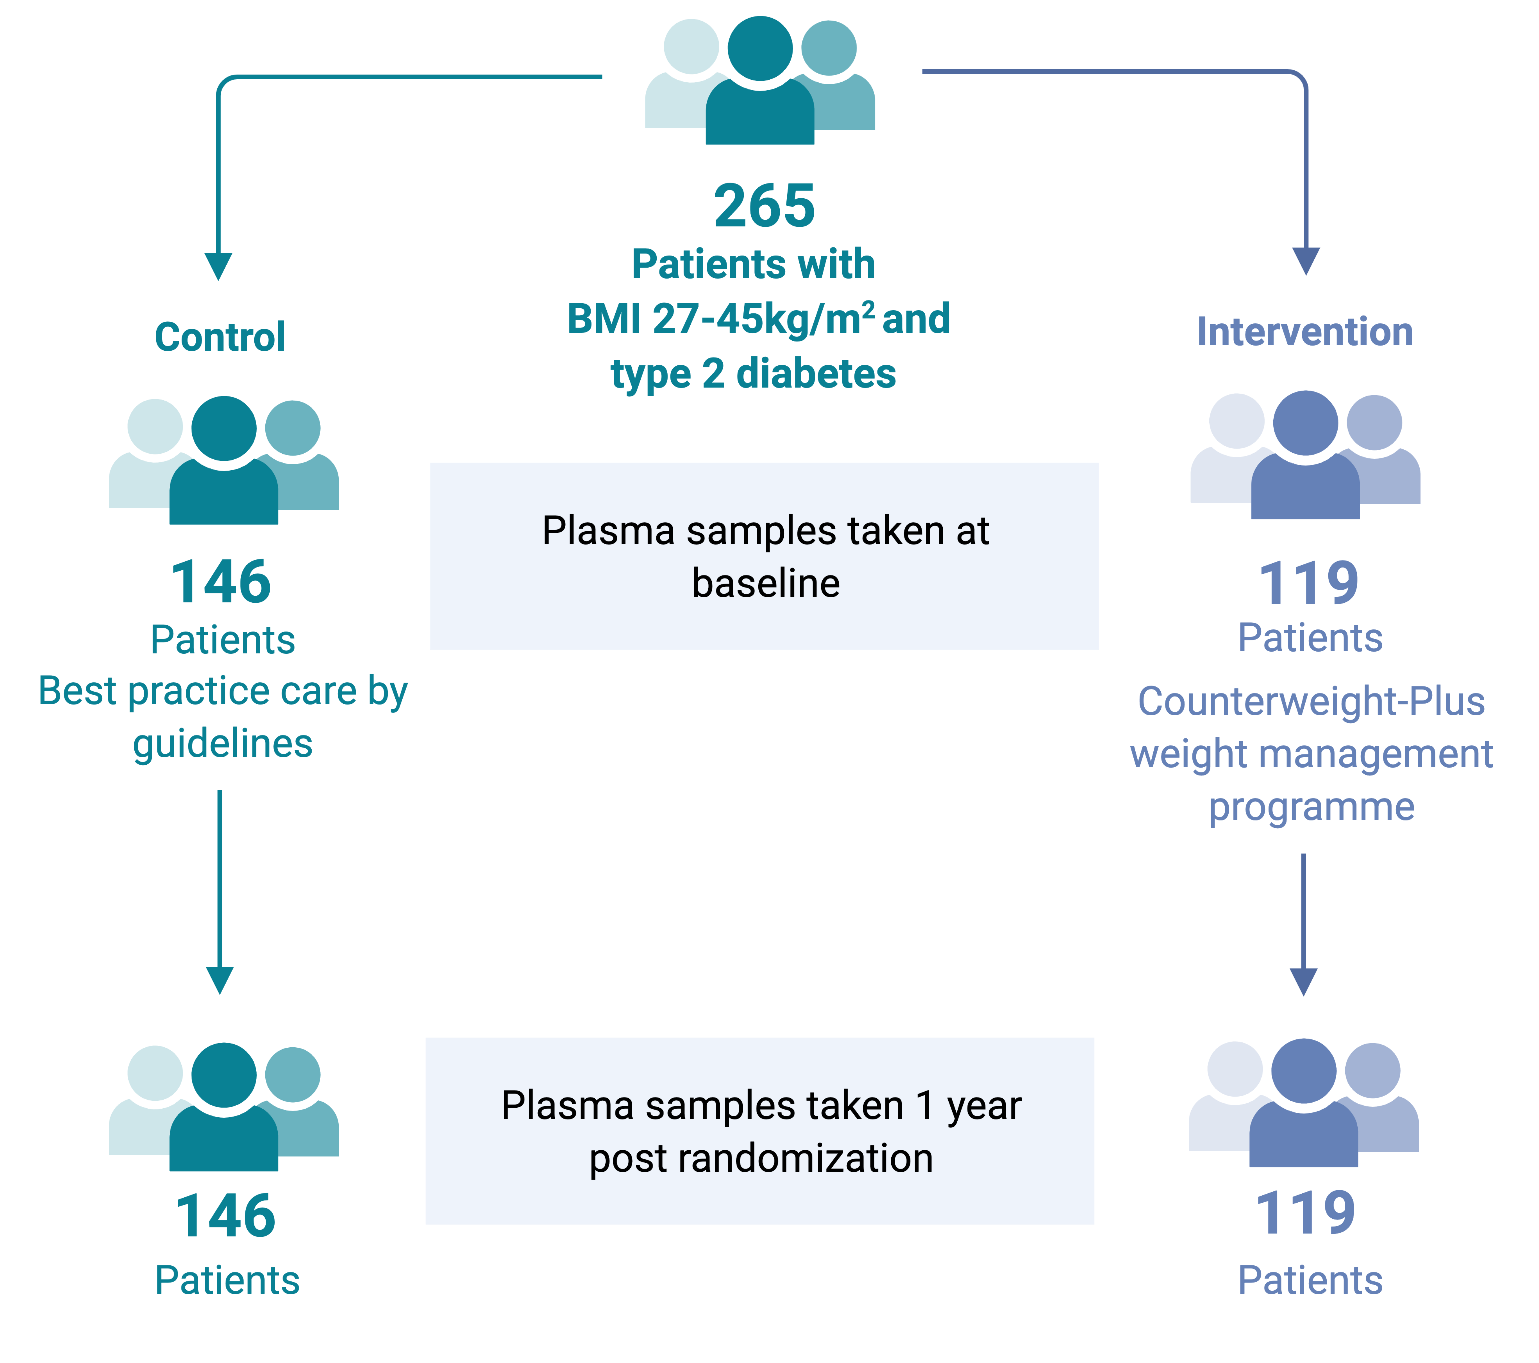
\includegraphics{figure/DiRECT/DiRECT_study_summary} 

}

\caption[Overview of participants in the DiRECT trial]{\textbf{Overview of participants in the DiRECT trial.} Figure made using BioRender.com.}\label{fig:direct-participants}
\end{figure}
\hypertarget{variables-included-in-analysis}{%
\subsection{Variables included in analysis}\label{variables-included-in-analysis}}

Age and sex were self-reported. Height was measured with the Frankfort plane horizontal, with a portable stadiometer (Chasmors Ltd, London). Weight was measured using Class 111 approved calibrated scales (Marsden Group UK)\textsuperscript{\protect\hyperlink{ref-Leslie2016}{182}}. Blood was donated at various timepoints including at baseline (week 0) and at 1 year (\textasciitilde week 52), where HDL cholesterol, triglycerides, HbA1c and plasma glucose were measured. Systolic blood pressure was measured with the patient seated, rested and with legs uncrossed for ≥5 mins. BMI was calculated by dividing the weight (kg) by the square of the height (m). BMI change was calculated by subtracting BMI at baseline from BMI at 1 year. This BMI change was rank normal transformed (function rntransform() from ``moosefun'' R package \url{https://github.com/hughesevoanth/moosefun/}). The centre attended and list size of the practice (\textgreater5700 or ≤5700) determined whether participants were allocated to control or intervention (minimisation variables) and therefore were recorded.

\hypertarget{proteomics}{%
\subsection{Proteomics}\label{proteomics}}

Blood was taken from participants into 9 mL vacutainers with EDTA (an anticoagulant) at baseline at and 1-year post-randomisation. Blood samples were centrifuged to derive plasma samples and plasma was stored at -80°C. Protein detection was performed by the SomaScan assay by SomaLogic. As mentioned before, this technique uses Slow Off-rate Modified Aptamers (SOMAmers) which make direct contact with proteins and quantifies protein levels by using a DNA microarray\textsuperscript{\protect\hyperlink{ref-Rohloff2014}{155}}. There were 5284 proteins included in the array, of which 4601 proteins passed internal quality control checks. The proteomic data was further cleaned using the ``metaboprep'' R package\textsuperscript{\protect\hyperlink{ref-Hughes2021}{184}}, with protein levels from both timepoints all QC'd together. This R package identified no extreme missingness (defined at 0.2 for sample and protein missingness), removed outliers (based on more than 5 SDs based on principal components (PCs) 1 and 2). The package also calculated the number of independent proteins by using pairwise correlation coefficients between proteins (869 representative proteins based on correlation coefficient of 0.5). The Shapiro-Wilk test was implemented to identify proteins which have a normal distribution (W≥0.95). Only 399 out of 4601 proteins had W statistics ≥0.95. As a result of this, all data was transformed to meet normality assumptions for analyses. This data log\textsubscript{2} transformed to match protein transformation by Sun et al.\textsuperscript{\protect\hyperlink{ref-Sun2018}{34}} then adjusted for age and sex (data had already undergone technical adjustment). Protein change was calculated for each individual by subtracting the baseline protein levels from protein levels at one-year. These protein change values were rank normal transformed.

\hypertarget{statistical-analysis-1}{%
\subsection{Statistical analysis}\label{statistical-analysis-1}}

Analyses were performed using R version 3.6.1. A total of 265 participants were included in the current analysis. Participant baseline characteristics were summarised as the mean and SD. Baseline characteristics were calculated for both control group (N=146) and intervention (N=119) and were compared across groups using either a two-tailed unpaired t-test or a Chi\textsuperscript{2} test.

The associations between BMI change and protein changes were explored using linear regression adjusting for centre, list size, age and sex (function lm() from base R ``stats'' package). Due to the nature of linear regression, outputs of regression provide the mean individual change in protein (in SDs) per SD increase in BMI. Therefore if more weight loss reduces the levels of protein, the beta coefficient is positive\textsuperscript{\protect\hyperlink{ref-Figarska2020}{185}}. The association between potential confounders (age and sex) and both exposure (BMI change) and outcome (protein change) were explored using linear regression. The difference in BMI change in intervention group compared to control was performed using linear regression, adjusting for centre, list size, age and sex. Covariables (age, sex, centre and list size) were compared across treatment groups. Treatment group was therefore used as an instrument for BMI change in a two stage least squares analysis \ref{fig:direct-tsls} to estimate the effects of BMI change on protein change using the ivreg() function from the ``AER'' R package (\url{https://github.com/cran/AER/blob/master/R/ivreg.R}). BMI change-protein change point estimates for 4601 proteins from the multiple linear regression analyses and two stage least squares analyses were compared using linear regression.

The association between BMI change and change in platelet proteins were also examined by searching for the UniProt IDs of the same platelet proteins as the previous chapter (Chapter \ref{BMI-protein-MR}). This approach was used due to the lack of distinct groupings in the SomaLogic protein list. As a sensitivity analysis, for proteins which associated with BMI change, baseline protein levels were compared across control and intervention groups. Similar to the previous chapter, the estimates for the effect of BMI change on a change in levels of the chemokines MDC and TARC were also explored. P-values were adjusted for multiple testing based on the number of representative proteins (0.05/869 = 5.8x10\textsuperscript{-5}). As a separate sensitivity analysis, a linear mixed model was used to account for baseline and endpoint protein levels (as the change in protein variable derived does not account for this). For the linear mixed model, the lmer() function from the ``lme4'' package, protein levels were used as the dependent variable, with treatment group and visit entered as fixed effects (and exploration of an interaction) and subject as a random effect. Estimates from the interaction of treatment group and visit were derived for each protein. These estimates were compared with the two stage least squares estimates.



\begin{figure}

{\centering 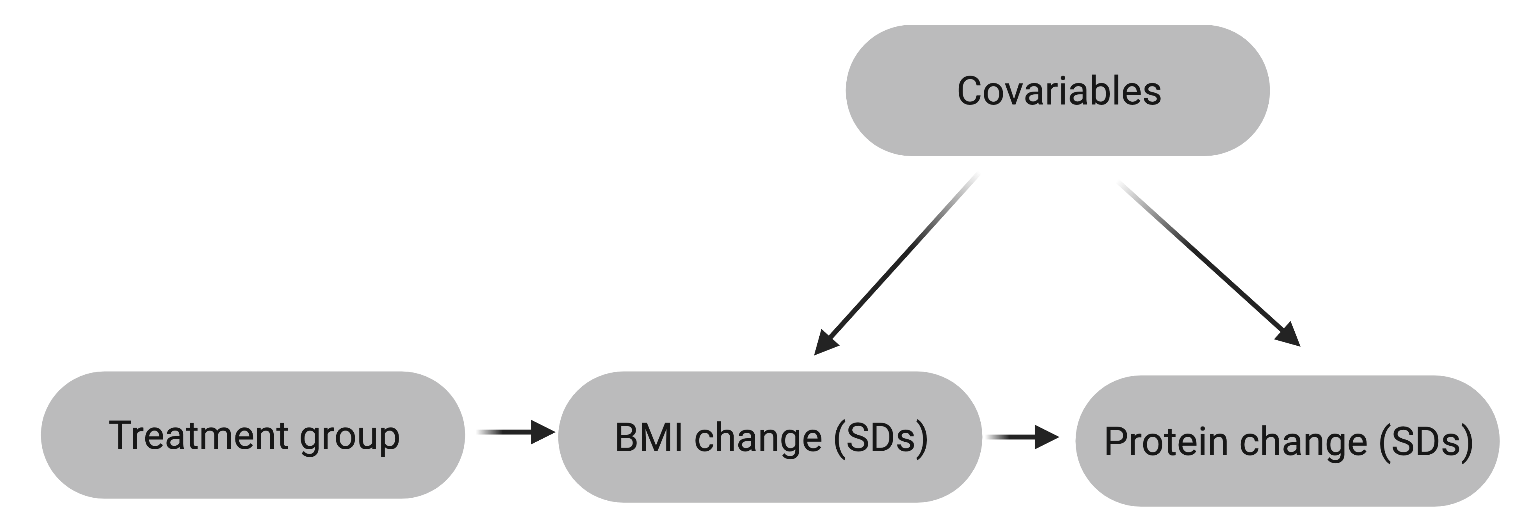
\includegraphics{figure/DiRECT/DiRECT_analysis} 

}

\caption[Schematic of two stage least squares analysis performed using DiRECT data]{\textbf{Schematic of two stage least squares analysis performed in the current chapter.} Figure made using BioRender.com.}\label{fig:direct-tsls}
\end{figure}
\hypertarget{disease-class-enrichment}{%
\subsection{Disease class enrichment}\label{disease-class-enrichment}}

Similarly to the previous chapters, proteins which had a BMI effect were taken forward into an enrichment analysis using DAVID Bioinformatics 6.8.\textsuperscript{\protect\hyperlink{ref-Huang2009}{157}} In total, 144 proteins were compared with all proteins detected (4601). Enrichment was explored by using the genetic association database (GAD). Enrichment was assessed by fold enrichment and by Bonferroni-corrected p-values. StringDB\textsuperscript{\protect\hyperlink{ref-Szklarczyk2021}{186}} was also used for a pathway enrichment analysis as DAVID Bioinformatics does not allow assigning of a rank order (such as by P value) to the input. Here the UniProt IDs of the proteins along with their -log\textsubscript{10} p value (smallest first) for both the observational analysis and the instrumental variable analysis. Pathway analysis was explored using gene ontology (GO) terms and KEGG pathways\textsuperscript{\protect\hyperlink{ref-Kanehisa2016}{187}}.

\hypertarget{results-4}{%
\section{Results}\label{results-4}}

\hypertarget{participant-characteristics-2}{%
\subsection{Participant characteristics}\label{participant-characteristics-2}}

Participants displayed similar characteristics across control and intervention groups (Table \ref{tab:DiRECT-participants}). Baseline BMI was similar across treatment groups (34.2 kg/m\textsuperscript{2} with SD of 4.3 kg/m\textsuperscript{2} in the control group vs 35.0 kg/m\textsuperscript{2} with SD of 4.6 kg/m\textsuperscript{2} in the intervention group, p=0.19). Other variables relating to cardiometabolic health were also similar across groups, including systolic blood pressure, HbA1c, glucose and insulin levels. The participants in the intervention group were younger and included fewer participants from Scotland but more from Tyneside.



\begin{landscape}\begin{table}

\caption[DiRECT participant characteristics]{\label{tab:DiRECT-participants}\textbf{DiRECT participant characteristics}}
\centering
\begin{tabu} to \linewidth {>{\raggedright\arraybackslash}p{6cm}>{\raggedright}X>{\raggedright}X>{\raggedright}X>{\raggedright}X>{\raggedright}X}
\toprule
Variable & Control mean (SD) or \% & Control N & Intervention mean (SD) or \% & Intervention N & P value for difference (Two tailed t-test or Chi2 test)\\
\midrule
Age & 56.2 (6.9) & 146 & 53.9 (7.1) & 119 & 0.01\\
Sex &  & 146 &  & 119 & 0.54\\
\hspace{1em}Male & 62 \% &  & 57 \% &  & \\
\hspace{1em}Female & 38 \% &  & 43 \% &  & \\
Body mass index (kg/m2) & 34.2 (4.3) & 146 & 35.0 (4.6) & 119 & 0.19\\
\addlinespace
Systolic Blood Pressue (mmHg) & 137 (15) & 146 & 135 (17) & 119 & 0.19\\
HbA1c (mmol/mol & 58 (11) & 146 & 60 (13) & 119 & 0.15\\
Glucose (mmol/l) & 8.8 (2.5) & 146 & 9.2 (3.2) & 118 & 0.24\\
Insulin (uu/ml) & 22 (14) & 146 & 24 (15) & 119 & 0.27\\
Cholesterol (mmol/l) & 4.3 (1.1) & 146 & 4.3 (1.1) & 118 & 0.9\\
\addlinespace
HDL (mmol/l) & 1.2 (0.3) & 146 & 1.1 (0.3) & 118 & 0.04\\
Triglycerides (mmol/l) & 1.9 (0.9) & 146 & 2.0 (1.4) & 118 & 0.48\\
Diabetes duration (years) & 3.0 (1.7) & 146 & 3.2 (1.6) & 119 & 0.37\\
Number of antidiabetic medications &  & 146 &  & 119 & 0.5\\
\hspace{1em}0 & 23 \% &  & 24 \% &  & \\
\addlinespace
\hspace{1em}1 & 53 \% &  & 44 \% &  & \\
\hspace{1em}2 & 18 \% &  & 23 \% &  & \\
\hspace{1em}3 & 5 \% &  & 7 \% &  & \\
\hspace{1em}4 & 1 \% &  & 3 \% &  & \\
Centre &  & 146 &  & 119 & 0.01\\
\addlinespace
\hspace{1em}Scotland & 77 \% &  & 62 \% &  & \\
\hspace{1em}Tyneside & 23 \% &  & 38 \% &  & \\
List size &  & 146 &  & 119 & 0.2\\
\hspace{1em}>5700 & 49 \% &  & 58 \% &  & \\
\hspace{1em}=<5700 & 51 \% &  & 42 \% &  & \\
\bottomrule
\end{tabu}
\end{table}
\end{landscape}
\hypertarget{observational-association-between-bmi-change-and-protein-change}{%
\subsection{Observational association between BMI change and protein change}\label{observational-association-between-bmi-change-and-protein-change}}

Linear regression was used to estimate the effect of BMI change on protein change, where BMI change (endpoint-baseline) was used as the exposure and protein change (endpoint-baseline) was used as the outcome and adjusting for confounders. After adjusting for multiple testing (p\textless5.8x10\textsuperscript{-5}), 254 proteins out of 4601 proteins were associated with BMI change (5.5 \% of all protein tested) (Supplementary Table 1). Although overall there was weight loss and a reduction in BMI, beta coefficients can be interpreted as the change in protein level (SDs) per SD increase in BMI. Negative associations were observed with BMI change and scavenger receptor class A member 5 (SCAR5, -0.62 SDs per SD increase in BMI, 95\% CI -0.72 to -0.53 p=3.7x10\textsuperscript{-29}) and apolipoprotein F (-0.58 SDs per SD increase in BMI, 95\% -0.68 to -0.48, p=1.8x10\textsuperscript{-24}). BMI change was positively associated with changes in levels of Proto-oncogene tyrosine-protein kinase receptor Ret (RET) (0.59 SDs increase per SD increase in BMI, 95\% CI 0.49 to 0.69 p=1.6x10\textsuperscript{-25}) and growth hormone receptor (GHR) (0.59 SDs increase per SD increase in BMI, 95\% CI 0.49 to 0.69 p=5.8x10\textsuperscript{-25}).

Proteins involved in GO platelet pathways were explored within the results. There were 248 platelet proteins identified in DiRECT. In the linear regression analysis, there was evidence for an effect of BMI change on 31 platelet proteins (12.5\%) (Supplementary Table 2). Associations include a positive association between BMI change and collagen type III (0.37 SDs increase per SD increase in BMI, 95\% CI 0.26-0.48), p=5.1x10\textsuperscript{-10}. There was also a positive association between BMI change and plasminogen activator inhibitor 1 (PAI-1, 0.29 SDs increase per SD increase BMI, 0.17-0.40, p=1.9x10\textsuperscript{-6}). The platelet primer insulin-like growth factor 1 (IGF-1) was negatively associated with BMI (-0.28 SDs per SD increase in BMI, 95\% CI -0.40 to -0.16, p=4.8x10\textsuperscript{-6}). The estimate for the association between BMI change and PAFAH was (-0.16 SDs per SD increase in BMI, 95\% CI -0.28 to -0.04, p=9.7x10\textsuperscript{-3}) and therefore did not pass multiple testing correction. The estimate for the effect of BMI change on the change in levels was 0.10 SD (95\% CI -0.02 to 0.22, p=0.099) and was 0.07 SD for TARC (95\% CI -0.04 to 0.19, p=0.22).

\hypertarget{association-between-confounders-and-exposureoutcomes}{%
\subsection{Association between confounders and exposure/outcomes}\label{association-between-confounders-and-exposureoutcomes}}

There was weak evidence for an association between age and BMI change (0.02 SDs increase in BMI change per 1 year, 95 \% CIs -0.0003 to 0.034, p=0.054), therefore indicating less weight loss with increasing age. There was no evidence that sex was associated with BMI change (BMI change 0.073 SDs increase in BMI change in females compared with males, 95 \% CI -0.17 to 0.32, p=0.56) (Supplementary Table 2). Age and sex displayed weak associations with protein changes, but these did not pass multiple testing adjustment (Supplementary Tables 3 and 4).

\hypertarget{association-between-treatment-group-and-bmi-change}{%
\subsection{Association between treatment group and BMI change}\label{association-between-treatment-group-and-bmi-change}}

Mean BMI change in all participants was -1.8kg/m\textsuperscript{2} (SD 2.5 kg/m\textsuperscript{2}), with a mean change in the control group of -0.4 kg/m\textsuperscript{2} (SD 1.3) vs -3.6kg/m\textsuperscript{2} (SD 2.5) in the intervention. The difference in BMI change comparing intervention to control was -3.2 kg/m\textsuperscript{2} (SE 0.25, p=1.52x10\textsuperscript{-29}). These analyses suggest that treatment group is a valid instrument for BMI change.



\begin{figure}

{\centering \includegraphics[width=0.85\linewidth]{figure/DiRECT/Intervention_BMI_change_boxplot} 

}

\caption[Box plot of the distribution of BMI change (kg/m\textsuperscript{2}) by treatment group]{\textbf{Box plot of the distribution of BMI change (kg/m\textsuperscript{2}) by treatment group}. Median and interquartile ranges displayed by the box. Dotted red line indicates where there is no change in BMI.}\label{fig:box-BMI-change}
\end{figure}
\hypertarget{two-stage-least-squares-analysis}{%
\subsection{Two-stage least squares analysis}\label{two-stage-least-squares-analysis}}

Treatment group was used as an instrument for BMI change in a two-stage least squares analysis. After adjustment for multiple testing, BMI change was associated with changes in levels of 171 proteins (3.7 \%) (Supplementary Table 5). The protein which showed the strongest association with BMI change was SCAR5 (-0.91 SDs per SD increase in BMI, 95\% CI -1.07 to -0.75, p=1.54x10\textsuperscript{-23}). Other proteins displayed a positive association with BMI change, including fatty acid-binding protein, heart (FABP1, 0.86 SDs increase per SD increase in BMI, 95\% CI 0.69-1.04, p=6.3x10\textsuperscript{-19}). Aminoacyclase-1 was also positively associated with BMI change (0.80 SDs increase in protein per SD increase in BMI, 95\% CI 0.64 to 0.97, p=4.9x10\textsuperscript{-18}). Figure \ref{fig:qq-plot-DiRECT} shows the qq-plot for the observational associations (A) and instrumental variable two stage least squares analysis (B). The protein with the smallest observed P value in both models is SCAR5, however the other ``top hits'' are not the same proteins in Figure \ref{fig:qq-plot-DiRECT}.



\begin{figure}

{\centering \includegraphics[width=1\linewidth]{figure/DiRECT/QQ_plots_obs_IV} 

}

\caption[QQ-plots of the expected vs the observed -log\textsubscript{10}(p-values) for the BMI change-protein change effects]{\textbf{QQ-plots of the expected vs the observed -log\textsubscript{10}(p-values) for the BMI change-protein change effects}. A) Linear regression B) Instrumental variable two stage least squares analysis.}\label{fig:qq-plot-DiRECT}
\end{figure}
In the two stage least squares analysis, there was evidence for an effect of BMI change on 13 platelet proteins. The estimate for the effect of BMI change on collagen type III was 0.53 SDs per SD increase in BMI (95\% CI 0.35 to 0.71, p=2.0x10\textsuperscript{-8}), larger in magnitude than in the observational analysis (Supplementary Table 2). The estimate for the association between BMI change and the platelet protein, PAFAH, strengthened in the instrumental variable model, where the estimate was -0.42 (95\% CI -0.61 to -0.22, p=5.3x10\textsuperscript{-5}), thereby passing the multiple testing adjustment. The two stage least squares analysis did not provide evidence for an effect of BMI change on a change in levels of MDC or TARC.

\hypertarget{comparison-of-observational-linear-regression-and-tsls-results-for-the-effect-of-bmi-change-on-protein-change}{%
\subsection{Comparison of observational linear regression and TSLS results for the effect of BMI change on protein change}\label{comparison-of-observational-linear-regression-and-tsls-results-for-the-effect-of-bmi-change-on-protein-change}}

A total of 110 proteins were only associated within the observational linear regression model, whereas 27 proteins were only associated in the TSLS analysis using treatment group as an instrument for BMI change. 144 proteins were associated with BMI in both analyses (\ref{fig:circos}), with largest effect estimates across methods for SCAR5, Adiponectin, Apolipoprotein F, growth hormone receptor (GHR), receptor-type tyrosine-protein phosphatase U (PTPRU) and sex hormone binding globulin. These can be seen in Figure \ref{fig:scatter-DiRECT}. Of these 144 BMI change-protein change associations that were consistent across both models, 121 were positive, where weight loss led to a reduction in levels of the protein.



\begin{figure}

{\centering 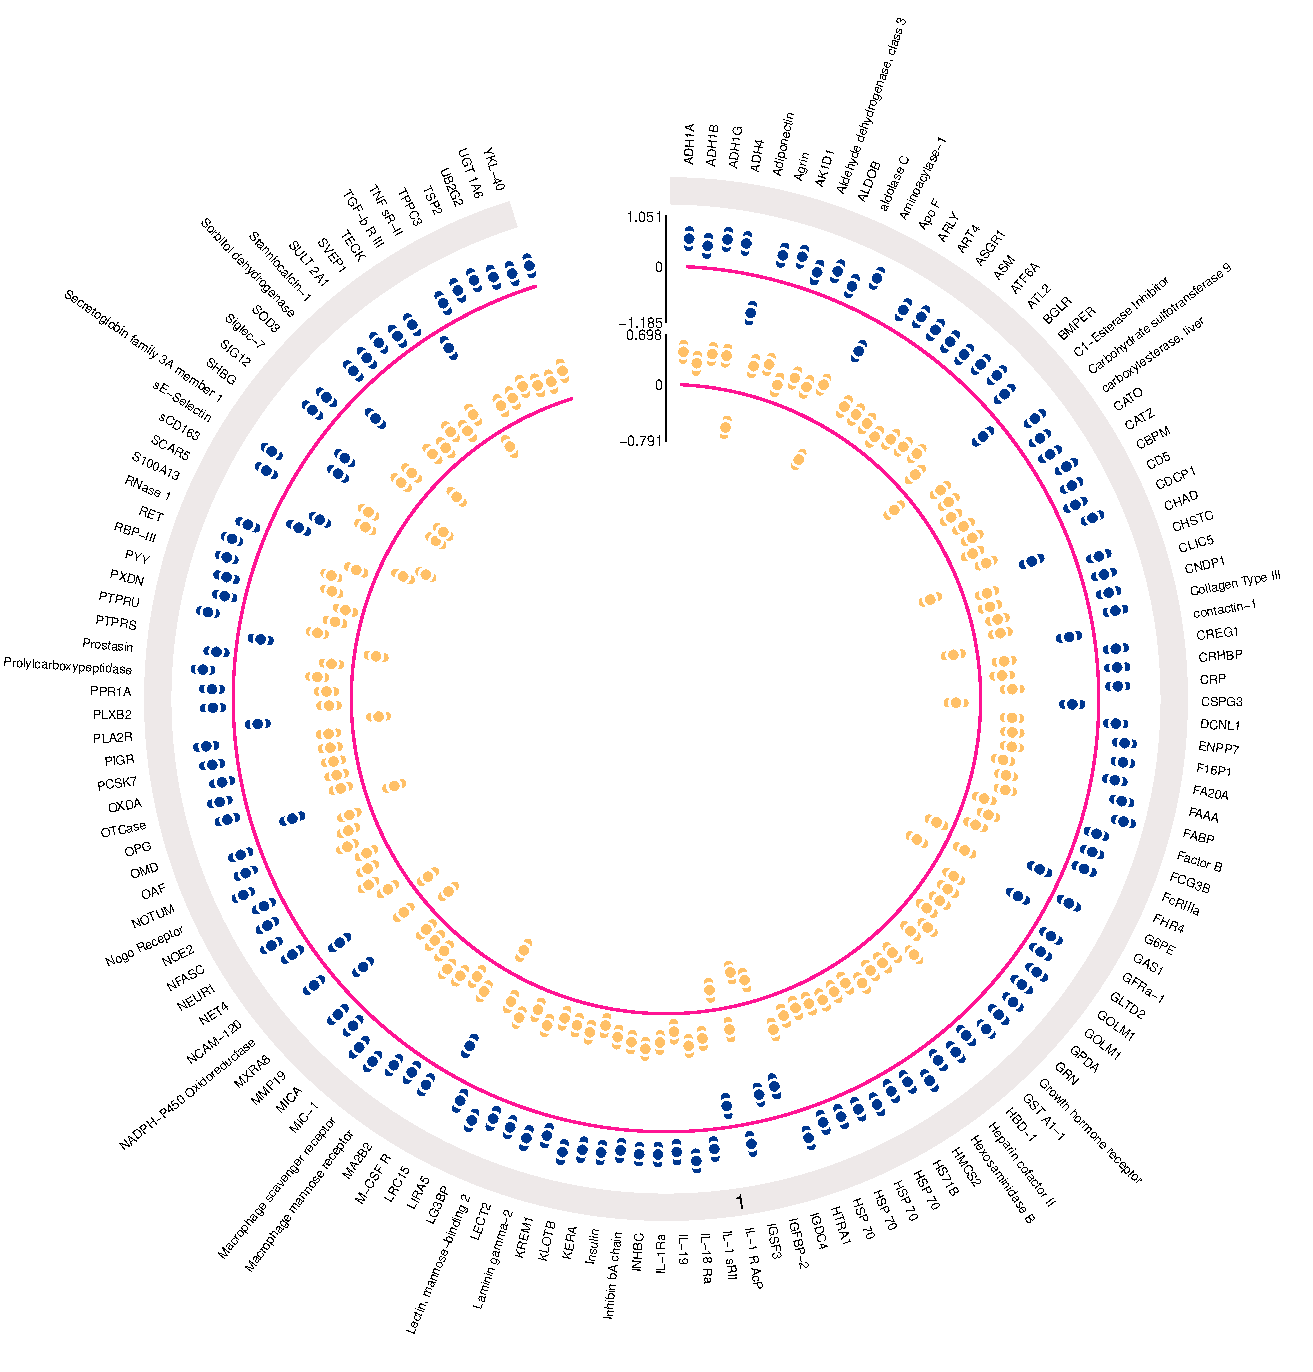
\includegraphics[width=0.8\linewidth]{figure/DiRECT/circos_plot_BMI_change_protein_ols_tsls} 

}

\caption[Circos plot of proteins associated with BMI change in DiRECT]{\textbf{Circos plot displaying the protein change (SDs) per SD increase in BMI in DiRECT}. Blue estimates are the two stage least squares estimates and the yellow estimates are from the linear regression. Proteins presented were associated in both models at p=5.8x10\textsuperscript{-5}. Figure made using the EpiViz R package \url{https://github.com/mattlee821/EpiViz}.}\label{fig:circos}
\end{figure}
\blandscape



\begin{figure}

{\centering \includegraphics[width=0.95\linewidth]{figure/DiRECT/DiRECT_scatter_comparison} 

}

\caption[Scatter plot comparing proteins association with BMI change across models in DiRECT]{\textbf{Scatter plot displaying the estimate for the change in protein (SDs) per SD increase in BMI in the two stage least squares and linear regression models.} Points are coloured by which models the proteins were associated with BMI change (p\textless5.8x10\textsuperscript{-5}).}\label{fig:scatter-DiRECT}
\end{figure}
\elandscape

\hypertarget{sensitivity-analysis}{%
\subsection{Sensitivity analysis}\label{sensitivity-analysis}}

\hypertarget{comparison-of-protein-levels-at-baseline-by-treatment-group}{%
\subsubsection{Comparison of protein levels at baseline by treatment group}\label{comparison-of-protein-levels-at-baseline-by-treatment-group}}

Proteins which were associated with BMI change were compared across control and intervention groups at baseline. This was done as the delta protein variable used in the regression model does not account for absolute levels of protein at baseline, therefore it is possible that the change in levels of protein may appear to be associating with BMI change due to differing basal protein levels across groups. There was not strong evidence for any differences in baseline levels of proteins (p\textless5.8x10\textsuperscript{-5}). However, there was weak evidence that levels of certain proteins, for example apolipoprotein F (beta=-0.20, SE=0.07, p=0.005) and carbohydrate sulfotransferase (beta=0.11, SE=0.04, p=0.006) were different in treatment group compared to control. Figure \ref{fig:ApoF-carb-boxplot} displays the boxplots for the distribution of levels of these proteins at both baseline and endpoint for the intervention and control group.



\begin{figure}

{\centering \includegraphics[width=0.9\linewidth]{figure/DiRECT/ApoF_carb_boxplots} 

}

\caption[Sensitivity analysis: boxplot of the levels of Apolipoprotein F and Carbohydrate Sulfotransferase at baseline and endpoint, grouped by treatment group.]{\textbf{Sensitivity analysis: boxplot of the levels of Apolipoprotein F and Carbohydrate Sulfotransferase at baseline and endpoint, grouped by treatment group.} Median and IQR is indicated by the box. Units are not rank normal transformed.}\label{fig:ApoF-carb-boxplot}
\end{figure}
\hypertarget{using-a-linear-mixed-model-to-estimate-effects-of-treatment-group-and-timepoint-on-protein-levels}{%
\subsubsection{Using a linear mixed model to estimate effects of treatment group and timepoint on protein levels}\label{using-a-linear-mixed-model-to-estimate-effects-of-treatment-group-and-timepoint-on-protein-levels}}

To account for individual protein levels at each timepoint, a linear mixed model was used to determine the effect of the intervention on protein levels. The estimate for the interaction between treatment group and timepoint were derived for each protein, which can be interpreted as difference in gradient of protein change comparing the intervention to control. Estimates were compared with the two stage least squares analysis results which provided an estimate for the effect of BMI change on protein change, using the treatment group as an instrument. Units across models are different as the TSLS estimates protein change per SD higher BMI, while the linear mixed model estimates the gradient of the protein comparing endpoint to baseline, therefore the gradient with a reduction in BMI. The estimates from the two models were strongly associated (R\textsuperscript{2} = 0.91, p\textless2.0x10\textsuperscript{-16}, F=49280, intercept=0.017) (Figure \ref{fig:tsls-lmer}). As a specific example using SCAR5, the estimate from the TSLS was that per SD increase in BMI, SCAR5 reduces by -0.91 SDs in BMI, 95\% CI -1.07 to -0.75, p=1.54x10\textsuperscript{-23}. The linear mixed model suggests that the estimated difference in gradient of protein change (comparing endpoint to baseline) comparing intervention to control is 0.92 SDs (95\% CI 0.75 to 1.09, t=10.8).



\begin{figure}

{\centering \includegraphics[width=0.9\linewidth]{figure/DiRECT/Comparison_TSLS_lmer} 

}

\caption[Scatter plot of the estimates from the TSLS and linear mixed model analyses]{\textbf{Scatter plot of the estimates from the TSLS and linear mixed model analyses}.}\label{fig:tsls-lmer}
\end{figure}
\hypertarget{enrichment-analysis-1}{%
\subsection{Enrichment analysis}\label{enrichment-analysis-1}}

To explore disease class enrichment, DAVID Bionformatics 6.8 was used\textsuperscript{\protect\hyperlink{ref-Huang2009}{157}}. As there was consistent evidence for a BMI effect on 144 proteins across both models in DiRECT, these were compared to the full 4601 protein panel. There was strongest evidence for enrichment in proteins involved in metabolic disease (1.4 fold enrichment, p=4.21x10\textsuperscript{-3}), with evidence for enrichment of renal disease (1.8 fold enrichment, p=1.02x10\textsuperscript{-2}). Cardiovascular disease had weak evidence for enrichment, but this association did not pass multiple testing correction.


\begin{landscape}\begin{table}

\caption{\label{tab:DAVID-enrichment-DiRECT}\textbf{DiRECT protein enrichment results for disease class using DAVID bioinformatics 6.8\textsuperscript{\protect\hyperlink{ref-Huang2009}{157}}}}
\centering
\begin{tabu} to \linewidth {>{\raggedright\arraybackslash}p{5cm}>{\raggedright}X>{\raggedright}X>{\raggedright}X>{\raggedright}X>{\raggedright}X>{\raggedright}X>{\raggedright}X>{\raggedright}X}
\toprule
Term (Genetic Association Database disease class) & Count & \% & List Total &   Population Hits & Population Total & Fold Enrichment & P Value & Bonferroni-adjusted P value\\
\midrule
Metabolic & 73 & 53 & 118 & 1451 & 3204 & 1.4 & 2.34E-04 & 4.21E-03\\
Renal & 34 & 24 & 118 & 518 & 3204 & 1.8 & 5.72E-04 & 1.02E-02\\
Neurological & 49 & 35 & 118 & 884 & 3204 & 1.5 & 9.61E-04 & 1.72E-02\\
Psych & 36 & 26 & 118 & 589 & 3204 & 1.7 & 1.38E-03 & 2.45E-02\\
Pharmacogenomic & 51 & 37 & 118 & 964 & 3204 & 1.4 & 2.11E-03 & 3.74E-02\\
\addlinespace
Cancer & 56 & 40 & 118 & 1093 & 3204 & 1.4 & 2.23E-03 & 3.94E-02\\
Reproduction & 25 & 18 & 118 & 381 & 3204 & 1.8 & 4.49E-03 & 7.79E-02\\
Normal variation & 16 & 12 & 118 & 209 & 3204 & 2.1 & 8.09E-03 & 1.36E-01\\
Aging & 21 & 15 & 118 & 324 & 3204 & 1.8 & 1.21E-02 & 1.96E-01\\
Cardiovascular & 56 & 40 & 118 & 1214 & 3204 & 1.2 & 2.51E-02 & 3.68E-01\\
\bottomrule
\end{tabu}
\end{table}
\end{landscape}
Using StringDB and inputting p values for the association between BMI change and each protein change, there was evidence for enrichment of KEGG pathways. Using the UniProt IDs and p-values from the linear regression analysis for BMI change and protein change, there was evidence that proteins altered by protein change in the linear regression model were involved in cytokine-cytokine receptor interaction (enrichment score = 0.14, pathway size = 282, p = 2.4x10\textsuperscript{-4}) and complement and coagulation cascades (enrichment score = 0.36, pathway size = 82, p = 9.8x10\textsuperscript{-4}). These were the only pathways associated with the ``top of the input'', therefore indicating enrichment of proteins most strongly associated with BMI change. There was also enrichment for platelet activation, however the analysis suggested that this enrichment was at the bottom of the protein list (enrichment score 4.9, pathway size 122, p=6.5x10\textsuperscript{-5}), therefore more proteins involved in platelet activation were not associated with BMI change. The network of proteins involved in platelet activation is shown in Figure \ref{fig:platelet-enrichment}. KEGG enrichment results were not available by inputting the ranked p values for the proteins from the instrumental variable analysis.

\blandscape
\thispagestyle{empty}




\begin{figure}

{\centering \includegraphics[width=0.75\linewidth]{figure/DiRECT/string_platelet_activation_network} 

}

\caption[Network of proteins in DiRECT which are involved in platelet activation.]{\textbf{Network of proteins in DiRECT which are involved in platelet activation}. Nodes represent individual proteins. The halo colour represents the rank of the protein where blue indicates the top of the list (most strongly associated with BMI change) and red indicates the bottom of the list. The edges indicate known interactions between proteins. Figure from made using string-db.org}\label{fig:platelet-enrichment}
\end{figure}
\elandscape

\hypertarget{discussion-4}{%
\section{Discussion}\label{discussion-4}}

In this chapter, a clinical trial implementing caloric restriction-induced weight loss was utilised as a second line of evidence to assess the effect of BMI on the plasma proteome. This analysis provided evidence for a broad effect of weight loss on the plasma proteome, providing results the effect of caloric restriction on the most extensive set of proteins to date.

The current study identified 144 BMI-related protein changes that were consistent across both models. This includes a reduction in BMI reducing levels of GHR, while increasing levels of apolipoprotein F, SHBG and IGFBP1/2. Table \ref{tab:weight-loss-protein} provides a summary of findings from the literature from previous studies which have explored the effect of caloric restriction on plasma proteins. As detailed in the table, previous studies have mainly used mass spectrometry. One study used SomaLogic\textsuperscript{\protect\hyperlink{ref-Carayol2017}{188}}, however this panel only included 1129 proteins. The current study utilised over fourfold more proteins, therefore providing more in depth readouts of biological processes. Findings are in concordance with previous studies\textsuperscript{\protect\hyperlink{ref-Figarska2020}{185},\protect\hyperlink{ref-Carayol2017}{188}--\protect\hyperlink{ref-Bruderer2019}{192}}. These protein changes replicate across cohorts and proteomic platforms and are more likely to be robust associations. Proteins altered with caloric restriction have been implicated in disease including coronary artery disease and T2D within the same cohort\textsuperscript{\protect\hyperlink{ref-Ritchie2019}{173}}. A mediation analysis suggested that proteins mediate the risk between a T2D genetic risk score (GRS) and incidence of T2D, such as IGFBP1/2, SHBG and GHR. Looking at individual proteins, a SNP which increases levels of ApoF also increases the risk of myocardial infarction and coronary heart disease\textsuperscript{\protect\hyperlink{ref-Liu2021}{139}}, therefore this apolipoprotein could contribute to the increased risk of thrombotic events seen with a higher BMI.



\begin{landscape}\begin{table}

\caption[Summary of current literature on the effect of weight loss on the plasma proteome]{\label{tab:weight-loss-protein}\textbf{Summary of current literature on the effect of weight loss on the plasma proteome}}
\centering
\begin{tabu} to \linewidth {>{\raggedright\arraybackslash}p{7cm}>{\raggedright}X>{\raggedright}X>{\raggedright\arraybackslash}p{8cm}}
\toprule
Paper & Author, year & Proteomic platform & Study summary\\
\midrule
Proteomics reveals the effects of sustained weight loss on the human plasma proteome & Geyer et al., 2016 & Mass spectrometry & Participants: 43 individuals with obesity before and after 8-week weight loss.
Total proteins associated: 93/1294,
Overlapping findings: Weight loss leads to increase in ApoF, ITIH3, SHBG, corticosteroid-binding globulin.\\
Proteomic profiles before and during weight loss: Results from randomized trial of dietary intervention & Figarska et al., 2020 & Olink CVD II, CVD III and inflammation & Participants: 609 from the diet intervention examining the factors interacting with treatment success (DIETFITS) study.
Total proteins associated: 130/26 associated with change in BMI.
Overlapping findings: Changes in IGFBP1/IGFBP2, E-selectin, CD163.\\
The differential plasma proteome of obese and overweight individuals undergoing a nutritional weight loss and maintenance intervention & Oller-Moreno et al., 2018 & Mass spectrometry & Participants: 473 in the nutritional programme DiOGenes.
Total proteins associated: 39/183.
Overlapping findings: Changes in SHBG, Adiponectin, IGFBP2, galectin-3-binding protein.\\
Integrative Personal Omics Profiles during Periods of Weight Gain and Loss & Piening et al., 2018 & Luminex and ProSeek by Olink & Participants: 23 with overweight or obesity undergoing weight loss.
Total proteins associated: 27/276.
Overlapping findings: changes in leptin.\\
Protein quantitative trait locus study in obesity during weight-loss identifies a leptin regulator & Carayol et al., 2017 & SomaLogic & Participants: 494 participants on low DiOGenes on low calorie diet.
Total proteins associated: 104/1129.
Overlapping findings: Changes in leptin, GHR, TIG2, IGFBP2, RET proto-oncogene (granulysin).\\
\addlinespace
Analysis of 1508 plasma samples by capillary-flow data-independent acquisition profiles proteomics of weight loss and maintenance & Bruderer et al., 2019 & Mass spectrometry & Participants: 477 in DiOGenes.
Total proteins associated: 271/465.
Overlapping findings: Changes in Apolipoprotein F, INHBC, SHBG.\\
\bottomrule
\end{tabu}
\end{table}
\end{landscape}
This study also provides some novel proteins associated with a reduction in BMI including SCAR5, chondroadherin (CHAD), fumarylacetoacetase (FAAA) and aminoacylase-1. A reduction in BMI led to an increase in plasma levels of SCAR5. This protein is involved in mediating commitment of mesenchymal stem cells into adipocytes and is highly expressed in white adipose tissue (WAT\textsuperscript{\protect\hyperlink{ref-Lee2017a}{193}}. A reduction in BMI also increased levels of chondroadherin (CHAD). Chondroadherin is a protein which is important in regulating exctracellular matrix organisation in cartilage and bones\textsuperscript{\protect\hyperlink{ref-Hessle2013}{194},\protect\hyperlink{ref-Iozzo2015}{195}}. CHAD knockout mice show decreased bone strength compared with wildtype\textsuperscript{\protect\hyperlink{ref-Hessle2013}{194}}. This suggests that weight reduction may be beneficial for bone strength. The function of these proteins and relationship with adiposity needs to be further characterised.

The effect of BMI on specific platelet-related proteins was explored by extracting the estimates for proteins involved in platelet GO pathways. Both analyses indicated that a reduction in BMI reduces the levels of collagen type III. Collagen activates platelets by binding to receptors such as the GPVI receptor, therefore this reduction may reduce platelet activation\textsuperscript{\protect\hyperlink{ref-Maurice2006}{196}}. The instrumental variable analysis detected an effect of BMI change on PAFAH. Here, a reduction in BMI led to higher levels of PAFAH. This platelet protein was detected in Chapter \ref{BMI-protein-MR}. PAFAH is protein which has been shown to bind to lipoproteins, thereby reducing their oxidation\textsuperscript{\protect\hyperlink{ref-Noto2003}{175}}. The comparison across studies will be discussed further in Chapter \ref{Comparison-proteome}. The chemokines utilised in Chapter \ref{chemokine-platelets}, MDC and TARC, were included in the SomaLogic panel, therefore were also specifically looked up within the results. The evidence suggested that a reduction in BMI did not alter levels of MDC and TARC, however it is also possible that the sample size was limited to detect smaller magnitudes of effects.

The enrichment results comparing the 144 proteins which were altered with BMI change to the full 4601 proteins tested confirmed this as there was strongest evidence for enrichment of proteins involved in metabolic disease and renal disease, however the effect on cardiovascular disease did not pass multiple testing adjustment. Pathway enrichment using StringDB also suggested that proteins most altered with BMI change were involved in cytokine-cytokine receptor interactions and complement and coagulation cascades, rather that platelet activation. It could be that the effect on inflammation and coagulation may be more immediate effects, and that changes in platelet activation may either require a more sustained weight loss, or a further reduction in BMI to see effects.

Limitations from the current analysis therefore include possible protein effects that are not caused by a change in BMI. Despite the use of the treatment group as an instrument in a two stage least squares analysis, the treatment group was also associated with an alteration in other factors: those who were allocated TDR also were taken off any T2D medication and were more likely to achieve remission of T2D. It is possible that the analysis is therefore picking up protein effects that are caused by a change in medication or T2D remission, rather than as a result in loss of fat. Participants would have also lost muscle mass throughout the intervention\textsuperscript{\protect\hyperlink{ref-Santanasto2011}{197}}, therefore it is not certain that effects are attributable to loss of fat. Despite this, there is evidence that in a group of participants with obesity, the majority of weight lost is fat mass\textsuperscript{\protect\hyperlink{ref-Backx2016}{198}}. Thirdly, BMI decreased by an average of 0.4kg/m\textsuperscript{2} in the control group and by 3.6 kg/m\textsuperscript{2}. As participants started at a mean BMI of 34-35 kg/m\textsuperscript{2}, the majority of participants will still have obesity even after the intervention. This may limit protein effects observed, as a certain BMI may need to be reached to see an alteration in protein levels (i.e.~the relationship may not be linear). Finally, it is unclear how generalisable results would be to the wider population. It is often the case with diets and caloric restriction that they only result in weight loss short-term and this is likely because the body adapts to the lower intake of calories. Therefore the changes which are seen in levels of proteins may not be so dynamic. The use of bariatric surgery may help to ensure weight loss and the associated changes are sustained.

Overall, this study provided evidence that weight loss leads to a substantial change in the composition of plasma proteins, replicating effects seen previously and providing some novel associations. Proteins altered with higher BMI in a Mendelian randomisation framework can be reversed with weight loss. Proteins altered with weight loss were enriched for renal disease and metabolic disease.

\hypertarget{Comparison-proteome}{%
\chapter{Combining MR and an RCT to determine effects of adiposity on the plasma proteome}\label{Comparison-proteome}}

\hypertarget{background-5}{%
\section{Background}\label{background-5}}

The two previous results chapters (Chapter \ref{BMI-protein-MR} and Chapter \ref{BMI-protein-RCT}) aimed to determine the effect of adiposity on circulating proteins by using two different study designs: an MR study which evaluated the effect that prolonged high BMI has on protein levels and an RCT which explored the effect of weight loss through caloric restriction on the plasma proteome. These two studies provided two separate line of evidence for a causal role of adiposity in circulating protein composition. Both studies also provided evidence that the change in circulating proteins may be contributing to the increased risk of disease such as metabolic disease or cardiovascular disease. There was also separate lines of evidence for an effect of BMI on certain proteins which may be important in platelet pathways.

This overall shift in proteins provides important information. One of the benefits of having the same proteomics platform in both studies is that there is a large overlap in the number of proteins measured. Each approach has its own biases and limitations and both the concordance and divergence in effects across studies provides insight into possible mechanisms. The overall aim of this chapter is to compare BMI-protein effects across MR and RCT study designs and evaluate implications for platelet function and cardiovascular disease.

\hypertarget{methods-4}{%
\section{Methods}\label{methods-4}}

In efforts to further elucidate which proteins are altered by adiposity, a comparison between the BMI-protein associations in INTERVAL (Chapter \ref{BMI-protein-MR}) and the BMI change-protein change associations in Chapter \ref{BMI-protein-RCT} was performed. There were 2803 unique proteins (by UniProt ID) which were detected in both INTERVAL and DiRECT. Estimates across the two cohorts were compared using linear regression. To be able to compare whether estimates were similar across study designs, estimates from each analysis were scaled using the scale() function from the ``base'' R package. Estimates were categorised as: similar if the scaled estimates were within 1 SD of each other; different if estimates were more than 1 SD apart and extreme if within 1 SD of each other and with an absolute scaled estimate of more than 1 SD.

Estimates for the specific platelet proteins highlighted in Chapters \ref{BMI-protein-MR} and \ref{BMI-protein-RCT} were also extracted to evaluate the effect of BMI on platelet proteins. Estimates were extracted from the MR interval and for the two stage least squares analysis in DiRECT as these were the more robust models.

\hypertarget{results-5}{%
\section{Results}\label{results-5}}

\hypertarget{comparison-of-bmi-effects-across-direct-and-interval}{%
\subsection{Comparison of BMI effects across DiRECT and INTERVAL}\label{comparison-of-bmi-effects-across-direct-and-interval}}

BMI-protein estimates from this DiRECT were compared with effect estimates from INTERVAL (Chapter \ref{BMI-protein-MR}), where 2803 proteins were detected across both studies. Both cohorts, through use of different study designs, provided evidence for an effect of BMI on the plasma proteome. Figure \ref{fig:DiRECT-INTERVAL} shows the BMI-protein estimates for the proteins which were included in both DiRECT and INTERVAL (R\textsuperscript{2}=0.11, P=1.0x10\textsuperscript{77}). There was consistent evidence across both studies that higher BMI leads to higher levels of various proteins including fumarylacetoacetase (FAAA), alcohol dehydrogenase 4 (ADH4), growth hormone receptor (GHR) and carboxypeptidase M (CBPM). Furthermore, higher BMI had a lowering effect on levels of sex hormone binding globulin (SHBG), as well as insulin-like growth factor binding protein 1/2 (IGFBP1/2). Although some of these estimates did not pass multiple testing in INTERVAL, the concordance in estimates in terms of effect size and direction of effect suggests that this is an issue of power.

\blandscape



\begin{figure}

{\centering \includegraphics[width=0.75\linewidth]{figure/DiRECT/DiRECT_INTERVAL_comparison} 

}

\caption[Scatter plot comparing the two stage least squares estimate for the effect of BMI change on protein change in DiRECT with the Mendelian randomisation estimate for the effect of BMI on protein levels in INTERVAL]{\textbf{Scatter plot comparing the two stage least squares estimate for the effect of BMI change on protein change in DiRECT with the Mendelian randomisation estimate for the effect of BMI on protein levels in INTERVAL.} Proteins that are similar across analyses with a large effect size in both studies are coloured in green, whereas those which display similar estimates across studies with small effect size are shown in blue. Proteins do not show similar effects across studies are shown in pink. A linear regression line is indicated in blue.}\label{fig:DiRECT-INTERVAL}
\end{figure}
\elandscape

The divergence in magnitude of estimates across study designs also suggests that some proteins are only associated with BMI in one study design. For example, the estimates in INTERVAL suggested that BMI has an effect on complement factors such as Complement C5 and Complement Factor I. As seen in Figure \ref{fig:DiRECT-INTERVAL-group}, these complement factors as well as others group together, where they appear to have a relationship with BMI in INTERVAL but are not affected by weight loss in DiRECT. There are other proteins which show the opposite: SCAR5 and CHAD displayed strong associations with BMI change in DiRECT, however the MR did not detect a causal effect of BMI on levels of these proteins \ref{fig:DiRECT-INTERVAL-group}.

\blandscape



\begin{figure}

{\centering \includegraphics[width=0.75\linewidth]{figure/DiRECT/DiRECT_INTERVAL_comparison_groups} 

}

\caption[Scatter plot comparing the two stage least squares estimate for the effect of BMI change on protein change in DiRECT with the Mendelian randomisation estimate for the effect of BMI on protein levels in INTERVAL, with proteins that differ across models highlighted]{\textbf{Scatter plot comparing the two stage least squares estimate for the effect of BMI change on protein change in DiRECT with the Mendelian randomisation estimate for the effect of BMI on protein levels in INTERVAL, with proteins that differ across models highlighted.} Proteins that are similar across analyses with a large effect size in both studies are coloured in green, whereas those which display similar estimates across studies with small effect size are shown in blue. Proteins do not show similar effects across studies are shown in pink. A linear regression line is indicated in blue. Complement factors which group together are circled in red at the top. SCAR5 and CHAD are also indicated.}\label{fig:DiRECT-INTERVAL-group}
\end{figure}
\elandscape

Across both INTERVAL and DiRECT, 170 unique platelet proteins were detected. The estimates for these proteins are shown in Figure \ref{fig:DiRECT-INTERVAL-platelet}. Overall, the estimates were associated with each other (R\textsuperscript{2}=0.19, p=1.1x10\textsuperscript{-9}), however there were divergences in estimates for some proteins. Despite this, there were consistencies for some proteins. PAFAH was associated with BMI in the observational analysis in INTERVAL. However, PAFAH did not pass multiple testing in the MR analysis. Despite this, the estimate was similar in magnitude to the observational estimate. PAFAH was also associated with BMI change in DiRECT in the instrumental variable analysis (Figure \ref{DiRECT-INTERVAL-platelet}). The direction of the effect indicated that higher BMI is associated with reduction in circulating PAFAH. In agreement with this, a reduction in BMI lead to levels of PAFAH increasing. The estimates for PAFAH were similar and can be seen in Figure \ref{fig:DiRECT-INTERVAL-platelet}. Consistencies in the estimates across the two study designs for other proteins, such as for complement factor B, suggest other effects that may be mediated by BMI that could affect platelet function.



\begin{figure}

{\centering \includegraphics[width=0.75\linewidth]{figure/DiRECT/Comparison_scatter_platelet_proteins} 

}

\caption[Scatter plot of the two stage least squares estimate in DiRECT and the Mendelian Randomisation estimates in INTERVAL and the for the effect of BMI on proteins involved in platelet pathways]{\textbf{Scatter plot of the two stage least squares estimate in DiRECT and the Mendelian Randomisation estimates in INTERVAL and the for the effect of BMI on proteins involved in platelet pathways}.}\label{fig:DiRECT-INTERVAL-platelet}
\end{figure}
\hypertarget{discussion-5}{%
\section{Discussion}\label{discussion-5}}

This chapter brought together results from two different analyses to determine effects of adiposity on the plasma proteome (INTERVAL in Chapter \ref{BMI-protein-MR} and DiRECT in Chapter \ref{BMI-protein-RCT}). Comparisons of protein effects across the different study designs points towards proteins of interest which may be involved in the development or progression of obesity-associated cardiometabolic disease. This chapter also collated the results for the proteins which have been implicated in pathways relevant to platelets.

The comparison of results from Chapter \ref{BMI-protein-MR}, which used MR and observational associations to assess the effect of average higher BMI across a population on average protein levels, with results from an RCT in Chapter \ref{BMI-protein-RCT} provides two separate lines of evidence to suggest a causal role of BMI in levels of various proteins. The analysis in INTERVAL suggested that proteins most altered by BMI were enriched for diseases such as cardiovascular disease and metabolic disease. As the estimates for the effect of BMI on proteins were consistent across both DiRECT and INTERVAL, this suggests that weight loss is able to reverse the protein changes observed with higher BMI, thereby potentially reducing disease risk. Although previous studies have identified BMI effects on some of these proteins, this direct comparison of effect estimates across an MR study design and weight loss intervention for the general proteome has not yet been done in this manner. This is a key strength of the study. The RCT had fewer participants than INTERVAL (265 vs 2737), but had enough power to detect an effect of BMI change on over 100 proteins. Proteins identified which would benefit following up, based on consistencies across study designs, include SHBG, IGFBP1/2, and GHR. The comparison has also highlighted some more novel proteins such as FAAA and PAFAH, which require further study.

Overall, estimates for the effect of BMI on platelet proteins in DiRECT and INTERVAL displayed a positive association. The agreement in effect estimates across study designs for the platelet protein PAFAH suggests that higher BMI does affect levels of this protein and that it is likely the power issue which means it cannot be detected in the MR. The power analysis in the discussion of Chapter \ref{BMI-protein-MR} supports this as it was calculated that an effect size of ±0.33 SDs would be required to have a power of 80\%. This protein has been suggested to be antiatherogenic, therefore lower levels would be proatherogenic\textsuperscript{\protect\hyperlink{ref-Noto2003}{175}}. There is also evidence in mice that knocking out PAFAH increases the weight of male mice, therefore indicating that PAFAH could be important in weight regulation\textsuperscript{\protect\hyperlink{ref-Nakamura2021}{199}}. A reverse MR analysis using SNPs associated with higher levels of PAFAH could help determine whether there is a likely causal role for PAFAH in weight regulation in humans. Validating this protein in an independent cohort and investigating this protein further in the lab could help reveal the functional implications of changes in PAFAH. This protein provides a good example of how triangulating can help tease apart the protein effects which are more likely to be driven by BMI.

Divergence in estimates across study designs may also suggest that there are spurious relationships occurring. However, this divergence may also provide some insight into the biology due to the nature of each study design. In general, the MR study design provides insight into the effect on the proteome that a sustained high BMI has over the life course and is therefore indicative of chronic effects. In contrast, the estimates in DiRECT are the effect that acute weight loss (1 year) has on the proteome. Complement factors may be altered in the MR study, but not after a weight loss intervention because weight loss may not have been sustained long enough to induce changes at the proteome level. There was no evidence for a causal relationship between BMI and both SCAR5 and CHAD in the MR, but these proteins displayed strong associations with weight loss in DiRECT. This could be because these protein changes are signals of starvation or due to other changes that happen with caloric restriction, such as a change of medication or loss of muscle mass. This requires further exploration, and requires more formal analysis to disentangle effects.

One of the limitations of the analyses performed in Chapter \ref{BMI-protein-MR} and Chapter \ref{BMI-protein-RCT} is that many proteins are not in the SOMAscan in both studies. Out of 4,034 SOMAmers in INTERVAL and 4601 SOMAmers in DiRECT, there were 2803 proteins in both. This means that there would be other proteins which would likely have reproducible effects across study (such as leptin). Therefore, this is limiting which proteins are discussed in the current chapter.

Overall, this chapter brought together two different study designs which aimed to determine the effect of adiposity on the plasma proteome. Through directly comparing the magnitude of estimates, this chapter identifies proteins which have the strongest evidence for a BMI effect (SHBG, IGFBP1/2, GHR, FAAA), as well as identifying a role of BMI in levels of circulating PAFAH, which may have implications for atherosclerosis. Divergence in estimates indicates effects which may be specific to one study design such as a causal effect of BMI on complement factors in the MR, but the inability to reverse these effects with weight loss. Replicating in other cohorts is now required to further understand these relationships.

\hypertarget{Discussion}{%
\chapter{Discussion}\label{Discussion}}

\hypertarget{summary-of-findings}{%
\section{Summary of findings}\label{summary-of-findings}}

The work presented in this thesis brought together an interdisciplinary approach to expand on previous literature to further explore the contribution of platelet function and the plasma proteome to obesity-related cardiovascular disease (Figure \ref{fig:Thesis-schematic-chaps}). The results and limitations from each individual results chapter have been discussed in the relevant chapters. This discussion chapter will recap the main findings from the thesis, address the overall strengths and limitations, discuss the wider clinical implications of findings as well as suggest future research to expand on this area of research.



\begin{figure}

{\centering \includegraphics[width=0.8\linewidth]{figure/General_discussion/Thesis_graphic_overview_chapters} 

}

\caption[Schematic of the multi-step pathway addressed in the thesis with chapter numbers where associations are explored]{\textbf{Schematic of the multi-step pathway addressed in the thesis with chapter numbers where associations are explored.} Figure made using BioRender.com.}\label{fig:Thesis-schematic-chaps}
\end{figure}
A summary of the main findings of the thesis is provided in Table \ref{tab:main-thesis-findings}. This thesis started with exploring the effect of BMI on platelet traits within a cohort of UK blood donors (INTERVAL) (Chapter \ref{BMI-platelets-INTERVAL}). This chapter provided evidence, using both observational and MR analyses, that higher BMI increases IPC. As INTERVAL did not have measures of platelet function, associations between IPC and whole blood platelet aggregation were explored with a cardiac surgery cohort (COPTIC). Here IPC and platelet aggregation were positively associated, independent of the overall platelet count. The next chapter (Chapter \ref{BMI-platelets-clinic}) sought to determine the effect of BMI on more detailed readouts of platelet function by designing a patient study, recruiting patients who were due to undergo bariatric surgery. Here, alterations in the platelet proteome were found which may have implications for platelet function and signalling. Follow-up experiments using other platelet function techniques, with a larger sample size, are now required. Chapter \ref{chemokine-platelets} examined the effect of the chemokines MDC and TARC on platelet function, chemokines which may be raised as a result of obesity-induced inflammation. MDC and TARC were found to potentiate PAR1-AP induced platelet function in washed platelets and MDC was able to cause platelet aggregation in PRP. This aggregation was found to be mediated by CCR4, with evidence that this receptor signals through G\textsubscript{q} coupling. There was MR evidence that higher levels of MDC could contribute to DVT and PE. Chapters \ref{BMI-protein-MR} and \ref{BMI-protein-RCT} both aimed to explore effects of adiposity on the plasma proteome. Chapter \ref{BMI-protein-MR} used observational and MR frameworks and found causal evidence for an effect of BMI on the plasma proteome whereas Chapter \ref{BMI-protein-RCT} used a weight loss intervention to explore effects of BMI on the plasma proteome. Chapter \ref{Comparison-proteome} brought together these study designs to identify consistent evidence for BMI effects on proteins. These analyses pointed towards proteins which may be important in obesity-related cardiovascular disease such as SHBG, fumarylacetoacetase and IGFBP1/2. Specific analysis of the effect of BMI on plasma proteins involved in platelet proteins also implicated proteins such as PAFAH which is altered by BMI and may lead to platelet hyperactivity.


\begin{table}

\caption{\label{tab:main-thesis-findings}Summary of main findings from the thesis}
\centering
\begin{tabu} to \linewidth {>{\raggedright\arraybackslash}p{4cm}>{\raggedright\arraybackslash}p{12cm}}
\toprule
Chapter & Main findings\\
\midrule
Chapter 3 & Higher body mass index (BMI) leads to higher immature platelet count (IPC) in a Mendelian randomization framework (INTERVAL). Within a cardiac surgery cohort (COPTIC), immature platelet count was positively associated with whole blood platelet aggregation.\\
Chapter 4 & Laboratory experiments were optimised to assess platelet function from patients. In the clinical pilot study, the effect of high BMI on platelet function was inconclusive, but there was evidence for a difference in levels of platelet proteins across BMI groups.\\
Chapter 5 & This study provided evidence that the chemokines MDC and TARC can potentiate PAR1-AP induced platelet function. The chemokines were also found to be able to activate platelets when applied alone. A two sample Mendelian randomization analysis implicated higher levels of MDC in deep vein thrombosis and pulmonary embolism.\\
Chapter 6 & Higher BMI has a causal effect on levels of proteins which circulate in the plasma. Proteins most altered by BMI were enriched for cardiovascular disease, metabolic disease and renal disease.\\
Chapter 7 & Weight loss as a result of caloric restriction has a substantial effect on the plasma proteome, with changes enriched for metabolic disease and renal disease.\\
\addlinespace
Chapter 8 & Proteins altered by higher BMI in Chapter 6 can be reversed with weight loss in Chapter 7.\\
\bottomrule
\end{tabu}
\end{table}
\hypertarget{strengths}{%
\section{Strengths}\label{strengths}}

As previously mentioned, this thesis has approached hypotheses using a range of study designs. Integrating clinical studies, basic science, cohort studies and trial data has been crucial to further understand the role of BMI in platelet function. This is therefore a strength of the current research. One of the major benefits of these techniques are that they are in line with the principles of the 3Rs (replacement, reduction and refinement). The thesis has made use of available human data from various cohorts to avoid use of animals in research (replacement).

\hypertarget{limitations}{%
\section{Limitations}\label{limitations}}

Although efforts were made to examine all of the associations within the pathway in Figure \ref{fig:Thesis-schematic-chaps}, this was only possible where there was available data or where it was possible to address hypotheses with specifically designed clinical or basic science experiments. Certain analyses were therefore limited by the availability of data. For example, it would have been beneficial to have platelet function measured within the INTERVAL cohort as this would have made it possible to do a one sample MR for BMI to platelet function, and the plasma proteome findings could have been directly compared to platelet function. Although platelet function data is not available on this scale, cohorts such as the Framingham Heart Study (FHS) have platelet function data for \textasciitilde3,000 participants\textsuperscript{\protect\hyperlink{ref-Rodriguez2020}{200}}. As they also have genetic data, it would be beneficial to perform a one sample MR for BMI to platelet function. The association between IPC and platelet function would benefit from being replicated in a larger cohort who are free from major disease such as the FHS, however this study does not have IPC measured.

As mentioned in Chapter \ref{BMI-platelets-clinic}, a major limitation is the lack of longitudinal data for the bariatric surgery and platelet function study. Before the COVID-19 pandemic, the experimental plan was to have bariatric patients with BMI \textgreater{} 40 kg/m\textsuperscript{2} and controls followed up at four time points. These time points were: baseline (2-3 weeks before surgery), after the very low energy diet (VLED) that precedes bariatric surgery (day of surgery), 6 weeks post-surgery and 12 months post-surgery. This would have allowed exploration of the change in an individual's platelet function with weight loss. Previous studies have researched the effect of obesity and bariatric surgery on platelet function\textsuperscript{\protect\hyperlink{ref-Barrachina2019}{99},\protect\hyperlink{ref-Dobrydneva2012}{201}}, but platelet function at four timepoints surrounding bariatric surgery has not yet been explored, more specifically before and after the VLED. This study aimed to add in a time point at 12 months, which is where there is evidence for maximal weight loss\textsuperscript{\protect\hyperlink{ref-Maciejewski2016}{202}}. Therefore this study would have been one of the most in depth platelet function studies for bariatric surgery. Although now not achievable within this PhD project, this study will be able to be taken forward by the Hers lab.

Another limitation of the thesis is that there was no stratification by sex in analyses and lab experiments. Where possible, analyses were adjusted for sex and therefore should help to reduce the confounding effect from this variable, however there may be a need to explore whether there are any sex specific effects. It is possible that BMI has different effects on the plasma proteome in males and females. Previous studies have identified sex differences in inflammatory protein changes in individuals with and without metabolic syndrome, for example adiponectin\textsuperscript{\protect\hyperlink{ref-TerHorst2020}{203}}. A difference in platelet reactivity between males and females has also been reported, where aggregation in response to a range of platelet agonists was is greater in females\textsuperscript{\protect\hyperlink{ref-Becker2006}{204}}. Similarly, it has been observed within the Hers lab that females may have platelets which are more susceptible to the priming effects by chemokines and other priming molecules. Future analyses would benefit from stratifying analyses by sex to further investigate any sex-specific effects, however larger sample sizes would be required.

\hypertarget{wider-implications-of-findings}{%
\section{Wider implications of findings}\label{wider-implications-of-findings}}

The research within this thesis has contributed to the understanding of mechanisms of obesity-related cardiovascular disease. As well as providing evidence for a role of body mass index in the production of immature platelets, the research surrounding IPC has wider implications. As mentioned in Chapter \ref{BMI-platelets-INTERVAL}, the standard full blood count used by the NHS does not include IPC. Similarly, more detailed blood counts from newer haematology analyzers also do not provide IPC within the summary, however it can be derived from IPF and PLT. The finding that IPC associates with whole blood platelet aggregation is important as it not only suggests that IPC should be considered in patients with obesity, but it could also be a useful biomarker of platelet hyperactivity across the population. Studies have indicated that there is a positive correlation between IPC and ADP-induced platelet aggregation in patients receiving either prasugrel or ticagrelor, therefore IPC could be used to predict which patients would be more responsive to antiplatelet treatment\textsuperscript{\protect\hyperlink{ref-Bernlochner2015a}{101}}.

As well as IPC having the potential to be a useful biomarker, various plasma proteins could also be biomarkers for patients with obesity who may be at a greater risk of cardiovascular events and metabolic disease. Using MR, various proteins altered by BMI as shown in Chapter \ref{BMI-protein-MR} have been implicated in disease. For example, in work by Constantinescu et al., analyses suggested that certain proteins altered with BMI may have a causal role in DVT, including INHBC (Reference Andrei's paper). Proteins such as INHBC could therefore be therapeutic targets. These proteins could also be potential biomarkers.

\hypertarget{future-studies}{%
\section{Future studies}\label{future-studies}}

Based on the findings of the research, there have been more questions which have been raised and would require further research. These will be discussed in the following paragraphs.

The MR in Chapter \ref{BMI-platelets-INTERVAL} provided MR evidence for a causal relationship between BMI and IPC. There was also a positive association between BMI and IPC within the cardiac surgery cohort and, although the magnitude of estimate was the same, this effect was weak, therefore this is potentially attributable to the modest sample size. It would be beneficial to validate this association within an independent cohort, such as UK Biobank. It would be useful to link IPC to medical records to be able to look at whether IPC is a predictor of cardiovascular events such as myocardial infarction or stroke. Mendelian randomization could also be implemented to look at the causal effect of IPC on cardiovascular outcomes. Once summary statistics become available for a GWAS of platelet function with a larger sample size, it would also be beneficial to do an MR analysis to explore the causal role of IPC in platelet function.

Following the findings of Chapter \ref{BMI-platelets-clinic}, although underpowered, it was observed that some bariatric patients with obesity had a high IPC, as high as 40\%. Therefore, this needs to be evaluated in more bariatric patients. There are other bariatric cohorts such as the Stratification of Obese PHenotypes to optimize future obesity therapy (SOPHIA) study which would likely have the relevant full blood count data to perform these analyses. Further characterisation of the immature platelets in patients with obesity within the laboratory is also now required. Here it is possible to look at the expression of P-selectin within the gated immature platelets\textsuperscript{\protect\hyperlink{ref-Bernlochner2015a}{101}}, to determine how this differs in obesity and people of normal weight. It is currently unclear why higher BMI would be linked to the production of more platelets, but the platelet proteomics experiment using mass spectrometry implicated that certain proteins which may be markers of platelet maturity may be altered in obesity. These proteins such as actin could be characterised further using laboratory experiments. Use of small-molecule proteolysis targeting chimeras (PROTACs)\textsuperscript{\protect\hyperlink{ref-Sledz2020}{205}}, which can degrade proteins in platelets would be one such method to determine their role. GWAS for protein levels tend to be measured in the plasma or serum. This may be missing important changes which could be involved in disease progression. For example, levels of certain proteins could be unaltered in the plasma, but changes within certain cells such as platelets would provide additional information. If GWAS were performed for platelet proteins, Mendelian randomization could be performed to identify how this could affect cardiovascular outcomes. However, this would be labour intensive.

Analyses explored both the platelet proteome and the plasma proteome in relation to body mass index. The effect of obesity on microparticles released from platelets activated by thrombin has also been explored\textsuperscript{\protect\hyperlink{ref-Grande2019}{130}}. A systematic comparison across these three proteomes could reveal how these proteomes relate to each other. For example, it could be possible to see whether specific proteins are affected in the same way in both platelets and plasma, or if there is a reciprocal relationship. Initial analyses on platelet proteomic data from patients with COVID-19 have identified that many plasma COVID-19 biomarkers are also altered in platelets (unpublished data from the Hers group). This may also be the case for other diseases such as MI/DVT and therefore requires further exploration.

The MR analysis in Chapter \ref{BMI-protein-MR} provided evidence for a causal effect of BMI on a range of proteins. There was also MR evidence that higher BMI raises IPC. Exploring the possibility of a bidirectional effect for both of these analysis would be important as it cannot be ruled out that certain proteins could be involved in processes involved in weight regulation, such as with PAFAH. It is unlikely that IPC would have a causal effect on BMI, however this would also need to be confirmed by use of a two sample MR. The possible effect of plasma proteins on IPC could also be explored using a two sample MR, using summary statistics for their respective GWAS. Another way to address the effects of proteins on IPC and platelet function could be to apply proteins such as fumarylacetoacetase, SHBG and leptin to megakaryocytes and to see whether there are changes in production of platelets compared to control. Proteins could also be applied in platelet aggregation experiments or \emph{in vitro} thrombosis to see whether these cause platelet hyperactivity.

Exploring individual proteins is useful in understanding disease risk, however further work on protein profiles is required as it is more likely a change in various proteins mediates the risk. Techniques to explore profiles are not well developed, however there are a few approaches which could be implemented. One such technique would be network MR, to be able to identify the relationship between proteins altered by BMI. This could help reveal whether there are any cascade effects, where an alteration in one protein may lead to downstream changes in other proteins and as such be at the top of the cascade. Another technique to begin unpicking profile effects could be exploring the effect of BMI on ratios between proteins. This technique has been used for metabolites, for example a single measure of the ratio between monounsaturated fats to polyunsaturated fats circulating in the blood is used\textsuperscript{\protect\hyperlink{ref-Carayol2017c}{206}}. It is unclear whether this technique would be suitable for proteomics data, and if it is, which proteins would be biologically meaningful to express as a ratio.

Linear MR is commonly used, however this may not always be the most appropriate method as there are often non-linear relationships, for example between BMI and mortality, where there is a J-shaped relationship\textsuperscript{\protect\hyperlink{ref-Sun2019}{207}}. Non-linearity has been observed for other associations, for example with vitamin D deficiency and CVD risk\textsuperscript{\protect\hyperlink{ref-Zhou2021}{208}}. Most studies have implemented linear models when looking at the effect of BMI on proteins/metabolites, however these relationships should be re-examined for non-linearity. Methods to do this are currently available, but they are not easily implementable on a large scale, such as when there are thousands of protein outcomes. Current methods such as the ``nlmr'' R package stratify estimates based on quantiles. As a result of this, the user cannot define their bounds of their strata and therefore makes it difficult to interpret results. The ``glsmr'' package was therefore developed to allow to do so and therefore provide estimates for causal effects in the predefined ranges of the exposure such as BMI. More detail and implementation of these packages is provided in Appendix \ref{Appendix-A}, with an example using the effect of BMI on levels of leptin. This analysis points towards a non-linear relationship between BMI and leptin. Preliminary analyses indicate that there are non-linear relationships with other proteins such as GHR and IGFBPs, where levels plateau after around 30-35kg/m\textsuperscript{2}. These non-linear relationships may indicate that a certain threshold needs to be achieved with weight loss to achieve a more favourable protein profile. This could have implications for disease risk reduction.
A limitation of this approach is that stratifying MR estimates reduces the power and therefore creates more imprecise estimates. Furthermore, when looking at the effects of obesity at the upper end of the distribution (e.g.~BMI range of 40-60 kg/m\textsuperscript{2}), there are fewer participants and therefore causing the same power issue. As a result, larger sample sizes would be needed with oversampling at the ends of the distributions to ensure sufficient power in each stratum. More recently, SomaLogic proteomic analysis has been performed om plasma samples from nearly 40,000 Icelanders\textsuperscript{\protect\hyperlink{ref-Ferkingstad2021}{209}}. Studies of this scale would help with stratifying into groups while maintaining power. Other studies such as the Qatar Biobank have higher rates of obesity than other cohorts, where 39\% have obesity and the mean BMI is 29 kg/m\textsuperscript{2}\textsuperscript{\protect\hyperlink{ref-AlKuwari2015}{210}}. Studies such as this would be more suitable for non-linear analyses.

The analyses in Chapter \ref{BMI-protein-RCT} utilised an RCT implementing caloric restriction to explore the effect of weight loss on the plasma proteome. As mentioned briefly within the limitations section of that chapter, the reduction in BMI was modest, so the majority of participants will still have obesity even 1 year after the intervention. It is also likely that this weight loss would not be sustainable long term. Therefore it may be difficult to determine the effects of reducing adiposity. Bariatric surgery is another intervention which typically causes a greater reduction in BMI. A previous study in adolescents indicated that a gastric bypass and sleeve gastrectomy resulted in a 3-year BMI reduction of 15 kg/m\textsuperscript{2}, around 30\% reduction of baseline BMI\textsuperscript{\protect\hyperlink{ref-Inge2016}{211}}. This drastic change in BMI would likely have a substantial effect on the plasma proteome. Previous studies have explored this and I plan to utilise some pilot data from the bariatric surgery trial, where serum samples from before and after surgery have been analysed by the new Olink Explore 1536 panel. This will provide estimates for the effect of bariatric surgery-induced weight loss on the serum proteome. These estimate can be compared alongside the estimates presented in Chapter \ref{Comparison-proteome}, where there is protein overlap.

\hypertarget{overall-conclusion}{%
\section{Overall conclusion}\label{overall-conclusion}}

Overall, this thesis has brought together a range of techniques to investigate the contribution of platelet function and the plasma proteome as possible mechanisms of obesity-related cardiovascular disease. There was evidence for a causal relationship between body mass index and IPC: the clinical utility of IPC as a biomarker of platelet reactivity needs to be further characterised. In order to explore potential mechanisms of effects, two chemokines were shown to modulate platelet function, thereby indicated the circulating proteome can affect platelet function. Subsequent analyses demonstrated a broad effect of BMI on plasma proteins, which were enriched for cardiovascular disease possibly exerts downstream effects on platelet function. Larger studies with platelet function data are required to further examine these relationships.

\appendix

\hypertarget{Appendix-A}{%
\chapter{Exploring non-linear associations between body mass index and plasma proteins}\label{Appendix-A}}

This appendix contains an example of non-linearity occurring for the association between body mass index (BMI) and levels of certain plasma proteins within the INTERVAL dataset. This analysis was performed as a result of an observation within the group and from published data\textsuperscript{\protect\hyperlink{ref-Li2021}{212}} that the effect of BMI on certain circulating metabolites such as LDL-C may be non-linear. Therefore it is likely that this is also the case with proteins: biologically, proteins might reach a threshold and therefore increasing BMI may lead to a plateau in the levels of the protein. Alternatively, certain technologies may reach a maximum in detection. The SomaLogic platform has a wide range of detection from femtomolar to micromolar\textsuperscript{\protect\hyperlink{ref-Lim2017}{213}}, therefore maximal detection could be reached. This possible non-linear relationship has not been accounted for in the linear models and Mendelian ramdomisation analyses performed in Chapter \ref{BMI-protein-MR}. Non-linearity may also explain why some proteins may be altered as a result of high BMI in the MR, but caloric restriction may not alter the levels of the same protein. There may be a certain BMI that needs to be reached before protein levels are altered therefore in DiRECT, as BMI remains in the obese category, effects may not be seen. Exploring non-linearity is ongoing, but this appendix provides an example of the exploration of a possible non-linear relationship between BMI (in kg/m\textsuperscript{2}) and levels of leptin.

\hypertarget{observational-association-between-bmi-and-leptin}{%
\section{Observational association between BMI and leptin}\label{observational-association-between-bmi-and-leptin}}

Data from the INTERVAL study was used as was described in Chapter \ref{BMI-protein-MR}. BMI was not rank normal transformed to help with interpretation of non-linearity. The association between BMI and leptin was explored observationally using both a linear model and a non-linear generalized additive model (GAM) (Figure \ref{fig:leptin-lm-GAM}). Here, using BMI as the exposure and leptin as the outcome (without covariables added in the model), there was evidence for a positive linear association between the two variables. However, the non-linear GAM indicated that after a BMI of around 40 kg/m\textsuperscript{2} the levels of leptin do not increase anymore. These two models were compared using an ANOVA (F test) with the hypothesis that the non-linear GAM is a better fit than the linear model, where a small P value indicates that the GAM is a better fit. For leptin, R\textsuperscript{2} for the linear model was 0.51 and it was 0.56 for the GAM, with a p value of (2.17x10\textsuperscript{-59}). This was the smallest p value comparing the two models for all 4,034 SOMAmers in INTERVAL, therefore indicating that the non-linear association is the most appropriate for leptin.



\begin{figure}

{\centering \includegraphics[width=0.8\linewidth]{figure/Appendix/leptin_nonlinear_obs} 

}

\caption[Linear model and generalized additive model of the association between BMI and leptin]{\textbf{Linear model (blue) and non-linear generalized additive model (red) of the association between BMI and leptin with 95\% confidence intervals.} The vertical lines indicate the mean BMI for each BMI category (in order of underweight, healthy, all, overweight, obese).}\label{fig:leptin-lm-GAM}
\end{figure}
\hypertarget{determining-non-linear-effects-using-tsls-mr-methods}{%
\section{Determining non-linear effects using TSLS MR methods}\label{determining-non-linear-effects-using-tsls-mr-methods}}

Non-linearity can be easily implemented using observational methods. However due to the nature of MR, regressing the genetic risk score on BMI provided estimates of genetically predicted BMI (the first stage of the TSLS analysis). The protein was then regressed on this genetically predicted BMI (second stage of TSLS) using a non-linear function, however, this covered a limited range of BMI as seen in Figure \ref{fig:leptin-lm-GAM-MR}. Therefore it was more difficult to interpret a causal non-linear effect over the full range of BMI observed in the population.



\begin{figure}

{\centering \includegraphics[width=0.8\linewidth]{figure/Appendix/leptin_nonlinear_MR} 

}

\caption[Linear model and generalized additive model of the association between BMI and leptin using Mendelian randomization]{Linear model and generalized additive model of the association between BMI and leptin using Mendelian randomization. Linear model (blue) and generalized additive model (red) of the association between BMI and leptin with 95\% confidence intervals. The vertical lines indicate the mean BMI for each BMI category (underweight, healthy, all, overweight, obese)}\label{fig:leptin-lm-GAM-MR}
\end{figure}
\hypertarget{using-non-linear-mr-package}{%
\section{Using non-linear MR package}\label{using-non-linear-mr-package}}

The non-linear MR package (``nlmr'') was also utilised to overcome this issue. This package utilises two methods: fractional polynomials and piecewise MR.\textsuperscript{\protect\hyperlink{ref-Staley2017}{214}} Fractional polynomials consist of metaregression of the localised average causal effect (LACE) estimates against the mean of the exposure in each stratum, whereas the piecewise MR estimates linear functions in a piecewise manner, where the gradient is the LACE estimate in each stratum. As indicated in Figure \ref{fig:leptin-nlmr}A, the fractional polynomial method with five quantiles suggested that the levels of leptin start to plateau with higher BMI. This effect was less clear using the piecewise method in Figure \ref{fig:leptin-nlmr}B, which also has been set to five quantiles. However, tests of non-linearity such as the fractional polynomial non-linearity p-value suggested that this fit is not better than a linear model (p=0.13). This was also the case using the Cochran Q test for both the fractional polynomial and piecewise linear model, where the p-values were both 0.62. LACE estimates suggest that the effect of BMI on leptin is strongest in the first quantile (Estimate = 0.20, 95\% CI 0.10 to 0.30, p=7.00x10\^{}-5). For the fifth quantile, the estimate is 0.12 (95\% CI 0.04 to 0.20, p=0.0020).



\begin{figure}

{\centering \includegraphics[width=0.9\linewidth]{figure/Appendix/leptin_nlmr_fracpoly_piecewise} 

}

\caption[Effects of BMI on levels of leptin using non-linear MR]{\textbf{Effects of BMI on levels of leptin using non-linear MR from the nlmr R package.\textsuperscript{\protect\hyperlink{ref-Staley2017}{214}}} A) fractional polynomial MR. B) Piecewise MR.}\label{fig:leptin-nlmr}
\end{figure}
\hypertarget{gam-and-linear-stratified-mr-glsmr}{%
\section{GAM and linear stratified MR (GLSMR)}\label{gam-and-linear-stratified-mr-glsmr}}

The issue with these methods is that it isn't possible to estimate the effect of a certain range of BMI on protein levels. This is important to be able to understand the range of BMI where certain effects on proteins are likely to occur. Therefore the package ``glsmr'' was created within the group by David Hughes. This package enables estimates to be derived for the effect of the exposure on the outcome for specified ranges in the exposure, using both observational associations and using Mendelian randomization. It also compares the linear and non-linear models. More details can be found here \url{https://github.com/hughesevoanth/glsmr}. The effects of BMI on leptin levels were further explored using this package. For this analysis the strata were defined as 18.5-25 kg/m\textsuperscript{2} (healthy), 25-30kg/m\textsuperscript{2} (overweight) and 30-40kg/m\textsuperscript{2} (obesity). Similar to Figures \ref{fig:leptin-lm-GAM} and \ref{fig:leptin-lm-GAM-MR}, Figures \ref{fig:leptin-glsmr}A and B indicate the observational and MR linear and non-linear GAMs with the comparison in model fit indicated by the p-values. Here, the non-linear GAM is a better fit than the linear model (p=5.4x10\textsuperscript{-43}), but this was not the case for the MR analysis (p=0.07). Figure \ref{fig:leptin-glsmr}C indicates how as the BMI category increases, the magnitude of the estimate became smaller, where the estimate was halved when comparing the obesity group (estimate=0.11 SD per kg/m\textsuperscript{2} higher BMI, 95\% CI 0.09 to 0.13, p=1.5510\textsuperscript{-21}) with the healthy BMI group (estimate = 0.23 SDs per kg/m\textsuperscript{2} higher BMI, 95 \% CI 0.20 to 0.26, p=2.110\textsuperscript{-59}). The point estimate also attenuated when comparing the obesity group with the healthy BMI group in the MR (Figure \ref{fig:leptin-glsmr}D).



\begin{figure}

{\centering \includegraphics[width=0.9\linewidth]{figure/Appendix/glsmr_plot_leptin} 

}

\caption[Observational and Mendelian randomization estimates for the effect of BMI on leptin stratified by BMI category.]{\textbf{Observational and Mendelian randomization estimates for the effect of BMI (kg/m\textsuperscript{2}) on leptin (SDs) stratified by BMI category.} Shaded areas display the ranges of BMI of each stratum: 18.5-25 (red), 25-30 (blue), 30-40 (green) A) Comparison between the fit of the non-linear and linear generalized additive models (GAMs) with age and sex as covariables. B) Comparison between the fit of the non-linear and linear generalized additive models (GAMs) with age and sex as covariables for the two stage least squares Mendelian randomization (MR) analysis. C) Stratified estimates for the observational association between BMI and leptin (beta is SD change in leptin per 1 kg/m\textsuperscript{2} increase in BMI). D) Stratified estimates for the MR estimates for the effect of BMI on leptin (beta is SD change in leptin per 1 kg/m\textsuperscript{2} increase in BMI). Black indicates the estimate has a p value of \textgreater0.05 and red indicates p\textless0.05. Strata estimates are presented as circles with the estimate for the complete dataset represented by a square.}\label{fig:leptin-glsmr}
\end{figure}
\hypertarget{conclusion}{%
\section{Conclusion}\label{conclusion}}

This appendix provided an example of how non-linearity between BMI and protein outcomes can be explored using observational and MR methods. The development of the ``glsmr'' R package will help to systematically characterise the nature of associations between BMI and levels of all circulating proteins in studies such as INTERVAL and DiRECT.

\backmatter

\hypertarget{references}{%
\chapter*{References}\label{references}}
\addcontentsline{toc}{chapter}{References}

\markboth{References}{References}

\noindent

\setlength{\parindent}{-0.20in}
\setlength{\leftskip}{0.20in}
\setlength{\parskip}{8pt}

\hypertarget{refs}{}
\begin{CSLReferences}{0}{0}
\leavevmode\hypertarget{ref-Blackburn2014}{}%
\CSLLeftMargin{1. }
\CSLRightInline{Blackburn, H. \& Jacobs, D. {Commentary: Origins and evolution of Body Mass Index (BMI): Continuing saga}. (2014). doi:\href{https://doi.org/10.1093/ije/dyu061}{10.1093/ije/dyu061}}

\leavevmode\hypertarget{ref-WHO1995}{}%
\CSLLeftMargin{2. }
\CSLRightInline{{Physical status: The use and interpretation of anthropometry}. (1995). doi:\href{https://doi.org/10.1093/ajcn/64.5.830}{10.1093/ajcn/64.5.830}}

\leavevmode\hypertarget{ref-Wade2018}{}%
\CSLLeftMargin{3. }
\CSLRightInline{Wade, K. H., Carslake, D., Sattar, N., Davey Smith, G. \& Timpson, N. J. {BMI and Mortality in UK Biobank: Revised Estimates Using Mendelian Randomization}. \emph{Obesity (Silver Spring)} \textbf{26}, 1796--1806 (2018).}

\leavevmode\hypertarget{ref-NCD-RisC2016}{}%
\CSLLeftMargin{4. }
\CSLRightInline{(NCD-RisC), N. C. D. R. F. C. {Trends in adult body-mass index in 200 countries from 1975 to 2014: a pooled analysis of 1698 population-based measurement studies with 19{{}}2 million participants}. \emph{Lancet} \textbf{387}, 1377--1396 (2016).}

\leavevmode\hypertarget{ref-Templin2019}{}%
\CSLLeftMargin{5. }
\CSLRightInline{Templin, T., Hashiguchi, T. C. O., Thomson, B., Dieleman, J. \& Bendavid, E. {The overweight and obesity transition from the wealthy to the poor in low- And middleincome countries: A survey of household data from 103 countries}. \emph{PLoS Medicine} (2019). doi:\href{https://doi.org/10.1371/journal.pmed.1002968}{10.1371/journal.pmed.1002968}}

\leavevmode\hypertarget{ref-Bluher2019}{}%
\CSLLeftMargin{6. }
\CSLRightInline{Blüher, M. {Obesity: global epidemiology and pathogenesis}. \emph{Nat Rev Endocrinol} \textbf{15}, 288--298 (2019).}

\leavevmode\hypertarget{ref-TheLancetPublicHealth2018}{}%
\CSLLeftMargin{7. }
\CSLRightInline{The Lancet Public Health. {Tackling obesity seriously: the time has come}. (2018). doi:\href{https://doi.org/10.1016/S2468-2667(18)30053-7}{10.1016/S2468-2667(18)30053-7}}

\leavevmode\hypertarget{ref-BritishHeartFoundation2021}{}%
\CSLLeftMargin{8. }
\CSLRightInline{British Heart Foundation. {Heart {\&} Circulatory Disease Statistics 2021}. (2021).}

\leavevmode\hypertarget{ref-Virani2021}{}%
\CSLLeftMargin{9. }
\CSLRightInline{Virani, S. S. \emph{et al.} {Heart Disease and Stroke Statistics---2021 Update}. \emph{Circulation} (2021).}

\leavevmode\hypertarget{ref-Khan2018}{}%
\CSLLeftMargin{10. }
\CSLRightInline{Khan, S. S. \emph{et al.} {Association of Body Mass Index With Lifetime Risk of Cardiovascular Disease and Compression of Morbidity}. \emph{JAMA Cardiol} \textbf{3}, 280--287 (2018).}

\leavevmode\hypertarget{ref-Nordestgaard2012}{}%
\CSLLeftMargin{11. }
\CSLRightInline{Nordestgaard, B. G. \emph{et al.} {The effect of elevated body mass index on ischemic heart disease risk: causal estimates from a Mendelian randomisation approach}. \emph{PLoS Med} \textbf{9}, e1001212 (2012).}

\leavevmode\hypertarget{ref-Davies2018}{}%
\CSLLeftMargin{12. }
\CSLRightInline{Davies, N. M., Holmes, M. V. \& Davey Smith, G. {Reading Mendelian randomisation studies: A guide, glossary, and checklist for clinicians}. \emph{BMJ (Online)} (2018). doi:\href{https://doi.org/10.1136/bmj.k601}{10.1136/bmj.k601}}

\leavevmode\hypertarget{ref-Gill2020}{}%
\CSLLeftMargin{13. }
\CSLRightInline{Gill, D., Walker, V. M., Martin, R. M., Davies, N. M. \& Tzoulaki, I. {Comparison with randomized controlled trials as a strategy for evaluating instruments in Mendelian randomization}. (2020). doi:\href{https://doi.org/10.1093/ije/dyz236}{10.1093/ije/dyz236}}

\leavevmode\hypertarget{ref-Bycroft2018}{}%
\CSLLeftMargin{14. }
\CSLRightInline{Bycroft, C. \emph{et al.} {The UK Biobank resource with deep phenotyping and genomic data}. \emph{Nature} (2018). doi:\href{https://doi.org/10.1038/s41586-018-0579-z}{10.1038/s41586-018-0579-z}}

\leavevmode\hypertarget{ref-Doney2009}{}%
\CSLLeftMargin{15. }
\CSLRightInline{Doney, A. S. F. \emph{et al.} {The FTO gene is associated with an atherogenic lipid profile and myocardial infarction in patients with type 2 diabetes :A Genetics of Diabetes Audit and Research Study in Tayside Scotland (Go-DARTS) Study}. \emph{Circulation: Cardiovascular Genetics} (2009). doi:\href{https://doi.org/10.1161/CIRCGENETICS.108.822320}{10.1161/CIRCGENETICS.108.822320}}

\leavevmode\hypertarget{ref-Bell2018}{}%
\CSLLeftMargin{16. }
\CSLRightInline{Bell, J. A. \emph{et al.} {Associations of Body Mass and Fat~Indexes~With Cardiometabolic Traits}. \emph{J Am Coll Cardiol} \textbf{72}, 3142--3154 (2018).}

\leavevmode\hypertarget{ref-Zhang1994}{}%
\CSLLeftMargin{17. }
\CSLRightInline{Zhang, Y. \emph{et al.} {Positional cloning of the mouse obese gene and its human homologue}. \emph{Nature} (1994). doi:\href{https://doi.org/10.1038/372425a0}{10.1038/372425a0}}

\leavevmode\hypertarget{ref-Friedman1998}{}%
\CSLLeftMargin{18. }
\CSLRightInline{Friedman, J. M. \& Halaas, J. L. {Leptin and the regulation of body weight in mammals}. (1998). doi:\href{https://doi.org/10.1038/27376}{10.1038/27376}}

\leavevmode\hypertarget{ref-Scuteri2007}{}%
\CSLLeftMargin{19. }
\CSLRightInline{Scuteri, A. \emph{et al.} {Genome-wide association scan shows genetic variants in the FTO gene are associated with obesity-related traits}. \emph{PLoS Genetics} (2007). doi:\href{https://doi.org/10.1371/journal.pgen.0030115}{10.1371/journal.pgen.0030115}}

\leavevmode\hypertarget{ref-Locke2015}{}%
\CSLLeftMargin{20. }
\CSLRightInline{Locke, A. E. \emph{et al.} {Genetic studies of body mass index yield new insights for obesity biology}. \emph{Nature} \textbf{518}, 197--206 (2015).}

\leavevmode\hypertarget{ref-Yengo2018}{}%
\CSLLeftMargin{21. }
\CSLRightInline{Yengo, L. \emph{et al.} {Meta-analysis of genome-wide association studies for height and body mass index in 700000 individuals of European ancestry}. \emph{Hum Mol Genet} \textbf{27}, 3641--3649 (2018).}

\leavevmode\hypertarget{ref-Bentzon2014}{}%
\CSLLeftMargin{22. }
\CSLRightInline{Bentzon, J. F., Otsuka, F., Virmani, R. \& Falk, E. {Mechanisms of plaque formation and rupture}. \emph{Circulation Research} (2014). doi:\href{https://doi.org/10.1161/CIRCRESAHA.114.302721}{10.1161/CIRCRESAHA.114.302721}}

\leavevmode\hypertarget{ref-Badimon2012}{}%
\CSLLeftMargin{23. }
\CSLRightInline{Badimon, L., Padró, T. \& Vilahur, G. {Atherosclerosis, platelets and thrombosis in acute ischaemic heart disease}. \emph{Eur Heart J Acute Cardiovasc Care} \textbf{1}, 60--74 (2012).}

\leavevmode\hypertarget{ref-Chernysh2020}{}%
\CSLLeftMargin{24. }
\CSLRightInline{Chernysh, I. N. \emph{et al.} {The distinctive structure and composition of arterial and venous thrombi and pulmonary emboli}. \emph{Scientific Reports} (2020). doi:\href{https://doi.org/10.1038/s41598-020-59526-x}{10.1038/s41598-020-59526-x}}

\leavevmode\hypertarget{ref-Koupenova2017a}{}%
\CSLLeftMargin{25. }
\CSLRightInline{Koupenova, M., Kehrel, B. E., Corkrey, H. A. \& Freedman, J. E. {Thrombosis and platelets: an update}. \emph{Eur Heart J} \textbf{38}, 785--791 (2017).}

\leavevmode\hypertarget{ref-Esmon2009}{}%
\CSLLeftMargin{26. }
\CSLRightInline{Esmon, C. T. {Basic mechanisms and pathogenesis of venous thrombosis}. \emph{Blood Reviews} (2009). doi:\href{https://doi.org/10.1016/j.blre.2009.07.002}{10.1016/j.blre.2009.07.002}}

\leavevmode\hypertarget{ref-Stone2017}{}%
\CSLLeftMargin{27. }
\CSLRightInline{Stone, J. \emph{et al.} {Deep vein thrombosis: Pathogenesis, diagnosis, and medical management}. (2017). doi:\href{https://doi.org/10.21037/cdt.2017.09.01}{10.21037/cdt.2017.09.01}}

\leavevmode\hypertarget{ref-Dale2017}{}%
\CSLLeftMargin{28. }
\CSLRightInline{Dale, C. E. \emph{et al.} {Causal Associations of Adiposity and Body Fat Distribution With Coronary Heart Disease, Stroke Subtypes, and Type 2 Diabetes Mellitus: A Mendelian Randomization Analysis}. \emph{Circulation} \textbf{135}, 2373--2388 (2017).}

\leavevmode\hypertarget{ref-Harshfield2021}{}%
\CSLLeftMargin{29. }
\CSLRightInline{Harshfield, E. L., Georgakis, M. K., Malik, R., Dichgans, M. \& Markus, H. S. {Modifiable Lifestyle Factors and Risk of Stroke: A Mendelian Randomization Analysis}. \emph{Stroke} (2021). doi:\href{https://doi.org/10.1161/STROKEAHA.120.031710}{10.1161/STROKEAHA.120.031710}}

\leavevmode\hypertarget{ref-Jimenez2021}{}%
\CSLLeftMargin{30. }
\CSLRightInline{Jiménez, A. \emph{et al.} {Weight-loss thresholds after bariatric surgery and cardiovascular outcomes: more is better}. \emph{International Journal of Obesity} (2021). doi:\href{https://doi.org/10.1038/s41366-021-00986-0}{10.1038/s41366-021-00986-0}}

\leavevmode\hypertarget{ref-Bell2018a}{}%
\CSLLeftMargin{31. }
\CSLRightInline{Bell, J. A. \emph{et al.} {Associations of Body Mass and Fat~Indexes~With Cardiometabolic Traits}. \emph{J Am Coll Cardiol} \textbf{72}, 3142--3154 (2018).}

\leavevmode\hypertarget{ref-Wurtz2014}{}%
\CSLLeftMargin{32. }
\CSLRightInline{Würtz, P. \emph{et al.} {Metabolic signatures of adiposity in young adults: Mendelian randomization analysis and effects of weight change}. \emph{PLoS Med} \textbf{11}, e1001765 (2014).}

\leavevmode\hypertarget{ref-Lu2014}{}%
\CSLLeftMargin{33. }
\CSLRightInline{Lu, Y. \emph{et al.} {Metabolic mediators of the effects of body-mass index, overweight, and obesity on coronary heart disease and stroke: A pooled analysis of 97 prospective cohorts with 1{{}}8 million participants}. \emph{The Lancet} (2014). doi:\href{https://doi.org/10.1016/S0140-6736(13)61836-X}{10.1016/S0140-6736(13)61836-X}}

\leavevmode\hypertarget{ref-Sun2018}{}%
\CSLLeftMargin{34. }
\CSLRightInline{Sun, B. B. \emph{et al.} {Genomic atlas of the human plasma proteome}. \emph{Nature} \textbf{558}, 73--79 (2018).}

\leavevmode\hypertarget{ref-Rivera2009}{}%
\CSLLeftMargin{35. }
\CSLRightInline{Rivera, J., Lozano, M. L., Navarro-Núñez, L. \& Vicente, V. {Platelet receptors and signaling in the dynamics of thrombus formation}. \emph{Haematologica} \textbf{94}, 700--711 (2009).}

\leavevmode\hypertarget{ref-Yau2015}{}%
\CSLLeftMargin{36. }
\CSLRightInline{Yau, J. W., Teoh, H. \& Verma, S. {Endothelial cell control of thrombosis}. \emph{BMC Cardiovasc Disord} \textbf{15}, 130 (2015).}

\leavevmode\hypertarget{ref-Gear2003}{}%
\CSLLeftMargin{37. }
\CSLRightInline{Gear, A. R. \& Camerini, D. {Platelet chemokines and chemokine receptors: linking hemostasis, inflammation, and host defense}. \emph{Microcirculation} \textbf{10}, 335--350 (2003).}

\leavevmode\hypertarget{ref-Durrant2017a}{}%
\CSLLeftMargin{38. }
\CSLRightInline{Durrant, T. N., Van Den Bosch, M. T. \& Hers, I. {Integrin \(\alpha\)IIb\(\beta\)3 outside-in signaling}. (2017). doi:\href{https://doi.org/10.1182/blood-2017-03-773614}{10.1182/blood-2017-03-773614}}

\leavevmode\hypertarget{ref-Huang2019}{}%
\CSLLeftMargin{39. }
\CSLRightInline{Huang, J. \emph{et al.} {Platelet integrin \(\alpha\)iIb\(\beta\)3: Signal transduction, regulation, and its therapeutic targeting}. (2019). doi:\href{https://doi.org/10.1186/s13045-019-0709-6}{10.1186/s13045-019-0709-6}}

\leavevmode\hypertarget{ref-Mehrbod2013}{}%
\CSLLeftMargin{40. }
\CSLRightInline{Mehrbod, M., Trisno, S. \& Mofrad, M. R. K. {On the activation of integrin \(\alpha\)iIb\(\beta\)3: Outside-in and inside-out pathways}. \emph{Biophysical Journal} (2013). doi:\href{https://doi.org/10.1016/j.bpj.2013.07.055}{10.1016/j.bpj.2013.07.055}}

\leavevmode\hypertarget{ref-Durrant2017}{}%
\CSLLeftMargin{41. }
\CSLRightInline{Durrant, T. N. \emph{et al.} {In-depth PtdIns(3,4,5)P}. \emph{Blood Adv} \textbf{1}, 918--932 (2017).}

\leavevmode\hypertarget{ref-Offermanns2006}{}%
\CSLLeftMargin{42. }
\CSLRightInline{Offermanns, S. {Activation of platelet function through G protein-coupled receptors}. (2006). doi:\href{https://doi.org/10.1161/01.RES.0000251742.71301.16}{10.1161/01.RES.0000251742.71301.16}}

\leavevmode\hypertarget{ref-Freynhofer2017a}{}%
\CSLLeftMargin{43. }
\CSLRightInline{Freynhofer, M. K. \emph{et al.} {Platelet turnover predicts outcome after coronary intervention}. \emph{Thromb Haemost} \textbf{117}, 923--933 (2017).}

\leavevmode\hypertarget{ref-Nardin2015}{}%
\CSLLeftMargin{44. }
\CSLRightInline{Nardin, M. \emph{et al.} {Body Mass Index and Platelet Reactivity During Dual Antiplatelet Therapy With Clopidogrel or Ticagrelor}. \emph{J Cardiovasc Pharmacol} \textbf{66}, 364--370 (2015).}

\leavevmode\hypertarget{ref-Khan2020}{}%
\CSLLeftMargin{45. }
\CSLRightInline{Khan, S. U. \emph{et al.} {Dual Antiplatelet Therapy after Percutaneous Coronary Intervention and Drug-Eluting Stents: A Systematic Review and Network Meta-Analysis}. \emph{Circulation} (2020). doi:\href{https://doi.org/10.1161/CIRCULATIONAHA.120.046308}{10.1161/CIRCULATIONAHA.120.046308}}

\leavevmode\hypertarget{ref-Warner2011}{}%
\CSLLeftMargin{46. }
\CSLRightInline{Warner, T. D., Nylander, S. \& Whatling, C. {Anti-platelet therapy: Cyclo-oxygenase inhibition and the use of aspirin with particular regard to dual anti-platelet therapy}. (2011). doi:\href{https://doi.org/10.1111/j.1365-2125.2011.03943.x}{10.1111/j.1365-2125.2011.03943.x}}

\leavevmode\hypertarget{ref-Degrauwe2017}{}%
\CSLLeftMargin{47. }
\CSLRightInline{Degrauwe, S. \emph{et al.} {Dual antiplatelet therapy for secondary prevention of coronary artery disease}. \emph{Open Heart} (2017). doi:\href{https://doi.org/10.1136/openhrt-2017-000651}{10.1136/openhrt-2017-000651}}

\leavevmode\hypertarget{ref-Grover2019}{}%
\CSLLeftMargin{48. }
\CSLRightInline{Grover, S. P. \& Mackman, N. {Intrinsic Pathway of Coagulation and Thrombosis}. \emph{Arteriosclerosis, Thrombosis, and Vascular Biology} (2019). doi:\href{https://doi.org/10.1161/atvbaha.118.312130}{10.1161/atvbaha.118.312130}}

\leavevmode\hypertarget{ref-Deharo2014}{}%
\CSLLeftMargin{49. }
\CSLRightInline{Deharo, P. \emph{et al.} {Body mass index has no impact on platelet inhibition induced by ticagrelor after acute coronary syndrome, conversely to prasugrel}. \emph{Int J Cardiol} \textbf{176}, 1200--1202 (2014).}

\leavevmode\hypertarget{ref-Sibbing2007}{}%
\CSLLeftMargin{50. }
\CSLRightInline{Sibbing, D., Beckerath, O. von, Schömig, A., Kastrati, A. \& Beckerath, N. von. {Impact of body mass index on platelet aggregation after administration of a high loading dose of 600 mg of clopidogrel before percutaneous coronary intervention}. \emph{Am J Cardiol} \textbf{100}, 203--205 (2007).}

\leavevmode\hypertarget{ref-Pankert2014}{}%
\CSLLeftMargin{51. }
\CSLRightInline{Pankert, M. \emph{et al.} {Impact of obesity and the metabolic syndrome on response to clopidogrel or prasugrel and bleeding risk in patients treated after coronary stenting}. \emph{Am J Cardiol} \textbf{113}, 54--59 (2014).}

\leavevmode\hypertarget{ref-Born1962}{}%
\CSLLeftMargin{52. }
\CSLRightInline{Born, G. V. R. {Aggregation of blood platelets by adenosine diphosphate and its reversal}. \emph{Nature} (1962). doi:\href{https://doi.org/10.1038/194927b0}{10.1038/194927b0}}

\leavevmode\hypertarget{ref-Chan2018}{}%
\CSLLeftMargin{53. }
\CSLRightInline{Chan, M. V., Armstrong, P. C. \& Warner, T. D. 96-well plate-based aggregometry. (2018). doi:\href{https://doi.org/10.1080/09537104.2018.1445838}{10.1080/09537104.2018.1445838}}

\leavevmode\hypertarget{ref-Toth2006}{}%
\CSLLeftMargin{54. }
\CSLRightInline{Tóth, O., Calatzis, A., Penz, S., Losonczy, H. \& Siess, W. {Multiple electrode aggregometry: A new device to measure platelet aggregation in whole blood}. \emph{Thrombosis and Haemostasis} (2006). doi:\href{https://doi.org/10.1160/TH06-05-0242}{10.1160/TH06-05-0242}}

\leavevmode\hypertarget{ref-Hu2017}{}%
\CSLLeftMargin{55. }
\CSLRightInline{Hu, L. \emph{et al.} {Platelets express activated P2Y12 receptor in patients with diabetes mellitus}. \emph{Circulation} (2017). doi:\href{https://doi.org/10.1161/CIRCULATIONAHA.116.026995}{10.1161/CIRCULATIONAHA.116.026995}}

\leavevmode\hypertarget{ref-Varga-Szabo2009}{}%
\CSLLeftMargin{56. }
\CSLRightInline{Varga-Szabo, D., Braun, A. \& Nieswandt, B. {Calcium signaling in platelets}. (2009). doi:\href{https://doi.org/10.1111/j.1538-7836.2009.03455.x}{10.1111/j.1538-7836.2009.03455.x}}

\leavevmode\hypertarget{ref-Bevers1983}{}%
\CSLLeftMargin{57. }
\CSLRightInline{Bevers, E. M., Comfurius, P. \& Zwaal, R. F. A. {Changes in membrane phospholipid distribution during platelet activation}. \emph{BBA - Biomembranes} (1983). doi:\href{https://doi.org/10.1016/0005-2736(83)90169-4}{10.1016/0005-2736(83)90169-4}}

\leavevmode\hypertarget{ref-Lisman2018}{}%
\CSLLeftMargin{58. }
\CSLRightInline{Lisman, T. {Platelet--neutrophil interactions as drivers of inflammatory and thrombotic disease}. (2018). doi:\href{https://doi.org/10.1007/s00441-017-2727-4}{10.1007/s00441-017-2727-4}}

\leavevmode\hypertarget{ref-Zarbock2007}{}%
\CSLLeftMargin{59. }
\CSLRightInline{Zarbock, A., Polanowska-Grabowska, R. K. \& Ley, K. {Platelet-neutrophil-interactions: Linking hemostasis and inflammation}. \emph{Blood Reviews} (2007). doi:\href{https://doi.org/10.1016/j.blre.2006.06.001}{10.1016/j.blre.2006.06.001}}

\leavevmode\hypertarget{ref-Hezard2005}{}%
\CSLLeftMargin{60. }
\CSLRightInline{Hezard, N. \emph{et al.} {Platelet VASP phosphorylation assessment in clopidogrel-treated patients: Lack of agreement between Western blot and flow cytometry}. \emph{Platelets} (2005). doi:\href{https://doi.org/10.1080/09537100500212551}{10.1080/09537100500212551}}

\leavevmode\hypertarget{ref-Horstrup1994}{}%
\CSLLeftMargin{61. }
\CSLRightInline{Horstrup, K. \emph{et al.} {Phosphorylation of focal adhesion vasodilator-stimulated phosphoprotein at Ser157 in intact human platelets correlates with fibrinogen receptor inhibition.} \emph{European journal of biochemistry} \textbf{225}, 21--27 (1994).}

\leavevmode\hypertarget{ref-Wang2013}{}%
\CSLLeftMargin{62. }
\CSLRightInline{Wang, P. \& Wilson, S. R. {Mass spectrometry-based protein identification by integrating de novo sequencing with database searching.} \emph{BMC bioinformatics} (2013). doi:\href{https://doi.org/10.1186/1471-2105-14-S2-S24}{10.1186/1471-2105-14-S2-S24}}

\leavevmode\hypertarget{ref-Huang2021}{}%
\CSLLeftMargin{63. }
\CSLRightInline{Huang, J. \emph{et al.} {Assessment of a complete and classified platelet proteome from genome-wide transcripts of human platelets and megakaryocytes covering platelet functions}. \emph{Scientific Reports} (2021). doi:\href{https://doi.org/10.1038/s41598-021-91661-x}{10.1038/s41598-021-91661-x}}

\leavevmode\hypertarget{ref-Gill2018}{}%
\CSLLeftMargin{64. }
\CSLRightInline{Gill, D., Monori, G., Georgakis, M. K., Tzoulaki, I. \& Laffan, M. {Genetically Determined Platelet Count and Risk of Cardiovascular Disease}. \emph{Arterioscler Thromb Vasc Biol} \textbf{38}, 2862--2869 (2018).}

\leavevmode\hypertarget{ref-Wurtz2012}{}%
\CSLLeftMargin{65. }
\CSLRightInline{Würtz, M., Hvas, A. M., Kristensen, S. D. \& Grove, E. L. {Platelet aggregation is dependent on platelet count in patients with coronary artery disease}. \emph{Thromb Res} \textbf{129}, 56--61 (2012).}

\leavevmode\hypertarget{ref-Femia2013}{}%
\CSLLeftMargin{66. }
\CSLRightInline{Femia, E. A., Scavone, M., Lecchi, A. \& Cattaneo, M. {Effect of platelet count on platelet aggregation measured with impedance aggregometry (Multiplate™ analyzer) and with light transmission aggregometry}. (2013). doi:\href{https://doi.org/10.1111/jth.12432}{10.1111/jth.12432}}

\leavevmode\hypertarget{ref-Furuncuoglu2016}{}%
\CSLLeftMargin{67. }
\CSLRightInline{Furuncuoğlu, Y. \emph{et al.} {How obesity affects the neutrophil/lymphocyte and platelet/lymphocyte ratio, systemic immune-inflammatory index and platelet indices: a retrospective study}. \emph{Eur Rev Med Pharmacol Sci} \textbf{20}, 1300--1306 (2016).}

\leavevmode\hypertarget{ref-Han2018a}{}%
\CSLLeftMargin{68. }
\CSLRightInline{Han, S. \emph{et al.} {Associations of Platelet Indices with Body Fat Mass and Fat Distribution}. \emph{Obesity (Silver Spring)} \textbf{26}, 1637--1643 (2018).}

\leavevmode\hypertarget{ref-Coban2005}{}%
\CSLLeftMargin{69. }
\CSLRightInline{Coban, E., Ozdogan, M., Yazicioglu, G. \& Akcit, F. {The mean platelet volume in patients with obesity}. \emph{Int J Clin Pract} \textbf{59}, 981--982 (2005).}

\leavevmode\hypertarget{ref-Heffron2018}{}%
\CSLLeftMargin{70. }
\CSLRightInline{Heffron, S. P., Marier, C., Parikh, M., Fisher, E. A. \& Berger, J. S. {Severe obesity and bariatric surgery alter the platelet mRNA profile}. \emph{Platelets} 1--8 (2018). doi:\href{https://doi.org/10.1080/09537104.2018.1536261}{10.1080/09537104.2018.1536261}}

\leavevmode\hypertarget{ref-Corpataux2020}{}%
\CSLLeftMargin{71. }
\CSLRightInline{Corpataux, N. \emph{et al.} {Reticulated platelets in medicine: Current evidence and further perspectives}. (2020). doi:\href{https://doi.org/10.3390/jcm9113737}{10.3390/jcm9113737}}

\leavevmode\hypertarget{ref-Ibrahim2014}{}%
\CSLLeftMargin{72. }
\CSLRightInline{Ibrahim, H. \emph{et al.} {Association of immature platelets with adverse cardiovascular outcomes}. \emph{J Am Coll Cardiol} \textbf{64}, 2122--2129 (2014).}

\leavevmode\hypertarget{ref-Maury2010a}{}%
\CSLLeftMargin{73. }
\CSLRightInline{Maury, E. \emph{et al.} {Effect of obesity on growth-related oncogene factor-alpha, thrombopoietin, and tissue inhibitor metalloproteinase-1 serum levels}. \emph{Obesity (Silver Spring)} \textbf{18}, 1503--1509 (2010).}

\leavevmode\hypertarget{ref-Frystyk1995}{}%
\CSLLeftMargin{74. }
\CSLRightInline{Frystyk, J., Vestbo, E., Skjaerbaek, C., Mogensen, C. E. \& Orskov, H. {Free insulin-like growth factors in human obesity}. \emph{Metabolism} \textbf{44}, 37--44 (1995).}

\leavevmode\hypertarget{ref-Hers2007}{}%
\CSLLeftMargin{75. }
\CSLRightInline{Hers, I. {Insulin-like growth factor-1 potentiates platelet activation via the IRS/PI3Kalpha pathway}. \emph{Blood} \textbf{110}, 4243--4252 (2007).}

\leavevmode\hypertarget{ref-Blair2015}{}%
\CSLLeftMargin{76. }
\CSLRightInline{Blair, T. A., Moore, S. F. \& Hers, I. {Circulating primers enhance platelet function and induce resistance to antiplatelet therapy}. \emph{J Thromb Haemost} \textbf{13}, 1479--1493 (2015).}

\leavevmode\hypertarget{ref-Pasquet2000}{}%
\CSLLeftMargin{77. }
\CSLRightInline{Pasquet, J. M. \emph{et al.} {Thrombopoietin potentiates collagen receptor signaling in platelets through a phosphatidylinositol 3-kinase-dependent pathway}. \emph{Blood} \textbf{95}, 3429--3434 (2000).}

\leavevmode\hypertarget{ref-Kowalska2000}{}%
\CSLLeftMargin{78. }
\CSLRightInline{Kowalska, M. A. \emph{et al.} {Stromal cell-derived factor-1 and macrophage-derived chemokine: 2 chemokines that activate platelets}. \emph{Blood} (2000). doi:\href{https://doi.org/10.1182/blood.v96.1.50}{10.1182/blood.v96.1.50}}

\leavevmode\hypertarget{ref-Abi-Younes2001}{}%
\CSLLeftMargin{79. }
\CSLRightInline{Abi-Younes, S., Si-Tahar, M. \& Luster, A. D. {The CC chemokines MDC and TARC induce platelet activation via CCR4}. \emph{Thromb Res} \textbf{101}, 279--289 (2001).}

\leavevmode\hypertarget{ref-Kitahara2014}{}%
\CSLLeftMargin{80. }
\CSLRightInline{Kitahara, C. M. \emph{et al.} {Body mass index, physical activity, and serum markers of inflammation, immunity, and insulin resistance}. \emph{Cancer Epidemiology Biomarkers and Prevention} (2014). doi:\href{https://doi.org/10.1158/1055-9965.EPI-14-0699-T}{10.1158/1055-9965.EPI-14-0699-T}}

\leavevmode\hypertarget{ref-Hemmings2015}{}%
\CSLLeftMargin{81. }
\CSLRightInline{Hemmings, B. A. \& Restuccia, D. F. {The PI3K-PKB/Akt pathway}. \emph{Cold Spring Harb Perspect Biol} \textbf{7}, (2015).}

\leavevmode\hypertarget{ref-Ezumi1998}{}%
\CSLLeftMargin{82. }
\CSLRightInline{Ezumi, Y., Uchiyama, T. \& Takayama, H. {Thrombopoietin potentiates the protein-kinase-C-mediated activation of mitogen-activated protein kinase/ERK kinases and extracellular signal-regulated kinases in human platelets}. \emph{Eur J Biochem} \textbf{258}, 976--985 (1998).}

\leavevmode\hypertarget{ref-VanWilligen2000}{}%
\CSLLeftMargin{83. }
\CSLRightInline{Willigen, G. van, Gorter, G. \& Akkerman, J. W. {Thrombopoietin increases platelet sensitivity to alpha-thrombin via activation of the ERK2-cPLA2 pathway}. \emph{Thromb Haemost} \textbf{83}, 610--616 (2000).}

\leavevmode\hypertarget{ref-Cercato2019}{}%
\CSLLeftMargin{84. }
\CSLRightInline{Cercato, C. \& Fonseca, F. A. {Cardiovascular risk and obesity}. (2019). doi:\href{https://doi.org/10.1186/s13098-019-0468-0}{10.1186/s13098-019-0468-0}}

\leavevmode\hypertarget{ref-Kern2001}{}%
\CSLLeftMargin{85. }
\CSLRightInline{Kern, P. A., Ranganathan, S., Li, C., Wood, L. \& Ranganathan, G. {Adipose tissue tumor necrosis factor and interleukin-6 expression in human obesity and insulin resistance}. \emph{American Journal of Physiology - Endocrinology and Metabolism} (2001). doi:\href{https://doi.org/10.1152/ajpendo.2001.280.5.e745}{10.1152/ajpendo.2001.280.5.e745}}

\leavevmode\hypertarget{ref-Esser2014}{}%
\CSLLeftMargin{86. }
\CSLRightInline{Esser, N., Legrand-Poels, S., Piette, J., Scheen, A. J. \& Paquot, N. {Inflammation as a link between obesity, metabolic syndrome and type 2 diabetes}. \emph{Diabetes Res Clin Pract} \textbf{105}, 141--150 (2014).}

\leavevmode\hypertarget{ref-Timpson2011}{}%
\CSLLeftMargin{87. }
\CSLRightInline{Timpson, N. J. \emph{et al.} {C-reactive protein levels and body mass index: elucidating direction of causation through reciprocal Mendelian randomization}. \emph{Int J Obes (Lond)} \textbf{35}, 300--308 (2011).}

\leavevmode\hypertarget{ref-Zaghlool2021}{}%
\CSLLeftMargin{88. }
\CSLRightInline{Zaghlool, S. B. \emph{et al.} {Revealing the role of the human blood plasma proteome in obesity using genetic drivers}. \emph{Nature Communications} (2021). doi:\href{https://doi.org/10.1038/s41467-021-21542-4}{10.1038/s41467-021-21542-4}}

\leavevmode\hypertarget{ref-Kalaoja2021}{}%
\CSLLeftMargin{89. }
\CSLRightInline{Kalaoja, M. \emph{et al.} {The Role of Inflammatory Cytokines as Intermediates in the Pathway from Increased Adiposity to Disease}. \emph{Obesity} (2021). doi:\href{https://doi.org/10.1002/oby.23060}{10.1002/oby.23060}}

\leavevmode\hypertarget{ref-Bretherick2020}{}%
\CSLLeftMargin{90. }
\CSLRightInline{Bretherick, A. D. \emph{et al.} {Linking protein to phenotype with Mendelian Randomization detects 38 proteins with causal roles in human diseases and traits}. \emph{PLoS Genetics} (2020). doi:\href{https://doi.org/10.1371/journal.pgen.1008785}{10.1371/journal.pgen.1008785}}

\leavevmode\hypertarget{ref-Noori2018}{}%
\CSLLeftMargin{91. }
\CSLRightInline{Noori, F., Naeimi, S., Zibaeenezhad, M. J. \& Gharemirshamlu, F. R. {CCL22 and CCR4 Gene Polymorphisms in Myocardial Infarction: Risk Assessment of rs4359426 and rs2228428 in Iranian Population}. \emph{Clin Lab} \textbf{64}, 907--913 (2018).}

\leavevmode\hypertarget{ref-Gold2012}{}%
\CSLLeftMargin{92. }
\CSLRightInline{Gold, L., Walker, J. J., Wilcox, S. K. \& Williams, S. {Advances in human proteomics at high scale with the SOMAscan proteomics platform}. \emph{N Biotechnol} \textbf{29}, 543--549 (2012).}

\leavevmode\hypertarget{ref-Cominetti2018}{}%
\CSLLeftMargin{93. }
\CSLRightInline{Cominetti, O. \emph{et al.} {Obesity shows preserved plasma proteome in large independent clinical cohorts}. \emph{Sci Rep} \textbf{8}, 16981 (2018).}

\leavevmode\hypertarget{ref-Imming2006}{}%
\CSLLeftMargin{94. }
\CSLRightInline{Imming, P., Sinning, C. \& Meyer, A. {Drugs, their targets and the nature and number of drug targets}. \emph{Nat Rev Drug Discov} \textbf{5}, 821--834 (2006).}

\leavevmode\hypertarget{ref-Bennett2017}{}%
\CSLLeftMargin{95. }
\CSLRightInline{Bennett, D. A. \& Holmes, M. V. {Mendelian randomisation in cardiovascular research: An introduction for clinicians}. (2017). doi:\href{https://doi.org/10.1136/heartjnl-2016-310605}{10.1136/heartjnl-2016-310605}}

\leavevmode\hypertarget{ref-Goudswaard2022}{}%
\CSLLeftMargin{96. }
\CSLRightInline{Goudswaard, L. J. \emph{et al.} {Higher body mass index raises immature platelet count: potential contribution to obesity-related thrombosis}. \emph{Platelets} 1--10 (2022). doi:\href{https://doi.org/10.1080/09537104.2021.2003317}{10.1080/09537104.2021.2003317}}

\leavevmode\hypertarget{ref-Wolk2003a}{}%
\CSLLeftMargin{97. }
\CSLRightInline{Wolk, R., Berger, P., Lennon, R. J., Brilakis, E. S. \& Somers, V. K. {Body mass index: a risk factor for unstable angina and myocardial infarction in patients with angiographically confirmed coronary artery disease}. \emph{Circulation} \textbf{108}, 2206--2211 (2003).}

\leavevmode\hypertarget{ref-Puurunen2018}{}%
\CSLLeftMargin{98. }
\CSLRightInline{Puurunen, M. K. \emph{et al.} {ADP Platelet Hyperreactivity Predicts Cardiovascular Disease in the FHS (Framingham Heart Study)}. \emph{J Am Heart Assoc} \textbf{7}, (2018).}

\leavevmode\hypertarget{ref-Barrachina2019}{}%
\CSLLeftMargin{99. }
\CSLRightInline{Barrachina, M. N. \emph{et al.} {GPVI surface expression and signalling pathway activation are increased in platelets from obese patients: Elucidating potential anti-atherothrombotic targets in obesity}. \emph{Atherosclerosis} \textbf{281}, 62--70 (2019).}

\leavevmode\hypertarget{ref-Lev2016a}{}%
\CSLLeftMargin{100. }
\CSLRightInline{Lev, E. I. {Immature Platelets: Clinical Relevance and Research Perspectives}. \emph{Circulation} \textbf{134}, 987--988 (2016).}

\leavevmode\hypertarget{ref-Bernlochner2015a}{}%
\CSLLeftMargin{101. }
\CSLRightInline{Bernlochner, I. \emph{et al.} {Impact of immature platelets on platelet response to ticagrelor and prasugrel in patients with acute coronary syndrome}. \emph{Eur Heart J} \textbf{36}, 3202--3210 (2015).}

\leavevmode\hypertarget{ref-Ibrahim2012}{}%
\CSLLeftMargin{102. }
\CSLRightInline{Ibrahim, H., Nadipalli, S., DeLao, T., Guthikonda, S. \& Kleiman, N. S. {Immature platelet fraction (IPF) determined with an automated method predicts clopidogrel hyporesponsiveness}. \emph{Journal of Thrombosis and Thrombolysis} (2012). doi:\href{https://doi.org/10.1007/s11239-011-0665-7}{10.1007/s11239-011-0665-7}}

\leavevmode\hypertarget{ref-Vaduganathan2008a}{}%
\CSLLeftMargin{103. }
\CSLRightInline{Vaduganathan, M. \emph{et al.} {Platelet reactivity and response to aspirin in subjects with the metabolic syndrome}. \emph{Am Heart J} \textbf{156}, 1002.e1--1002.e7 (2008).}

\leavevmode\hypertarget{ref-Mijovic2015a}{}%
\CSLLeftMargin{104. }
\CSLRightInline{Mijovic, R. \emph{et al.} {Reticulated platelets and antiplatelet therapy response in diabetic patients}. \emph{J Thromb Thrombolysis} \textbf{40}, 203--210 (2015).}

\leavevmode\hypertarget{ref-DiAngelantonio2017}{}%
\CSLLeftMargin{105. }
\CSLRightInline{Di Angelantonio, E. \emph{et al.} {Efficiency and safety of varying the frequency of whole blood donation (INTERVAL): a randomised trial of 45 000 donors}. \emph{Lancet} \textbf{390}, 2360--2371 (2017).}

\leavevmode\hypertarget{ref-Astle2016}{}%
\CSLLeftMargin{106. }
\CSLRightInline{Astle, W. J. \emph{et al.} {The Allelic Landscape of Human Blood Cell Trait Variation and Links to Common Complex Disease}. \emph{Cell} \textbf{167}, 1415--1429.e19 (2016).}

\leavevmode\hypertarget{ref-Purcell2007a}{}%
\CSLLeftMargin{107. }
\CSLRightInline{Purcell, S. \emph{et al.} {PLINK: a tool set for whole-genome association and population-based linkage analyses}. \emph{Am J Hum Genet} \textbf{81}, 559--575 (2007).}

\leavevmode\hypertarget{ref-Akbari2020}{}%
\CSLLeftMargin{108. }
\CSLRightInline{Akbari, P. \emph{et al.} {Genetic Analyses of Blood Cell Structure for Biological and Pharmacological Inference}. \emph{bioRxiv} 2020.01.30.927483 (2020). doi:\href{https://doi.org/10.1101/2020.01.30.927483}{10.1101/2020.01.30.927483}}

\leavevmode\hypertarget{ref-Team2019a}{}%
\CSLLeftMargin{109. }
\CSLRightInline{Team, R. C. {R: A language and environment for statistical computing. R Foundation~ for Statistical Computing, Vienna, Austria. URL https://www.R-project.org/.} (2019).}

\leavevmode\hypertarget{ref-Henningsen2007}{}%
\CSLLeftMargin{110. }
\CSLRightInline{Henningsen, A. \& Hamann, J. D. {Systemfit: A package for estimating systems of simultaneous equations in R}. \emph{Journal of Statistical Software} (2007). doi:\href{https://doi.org/10.18637/jss.v023.i04}{10.18637/jss.v023.i04}}

\leavevmode\hypertarget{ref-Mumford2017}{}%
\CSLLeftMargin{111. }
\CSLRightInline{Mumford, A. D. \emph{et al.} {Near-patient coagulation testing to predict bleeding after cardiac surgery: a cohort study}. \emph{Research and Practice in Thrombosis and Haemostasis} (2017). doi:\href{https://doi.org/10.1002/rth2.12024}{10.1002/rth2.12024}}

\leavevmode\hypertarget{ref-Grove2011a}{}%
\CSLLeftMargin{112. }
\CSLRightInline{Grove, E. L., Hvas, A. M., Mortensen, S. B., Larsen, S. B. \& Kristensen, S. D. {Effect of platelet turnover on whole blood platelet aggregation in patients with coronary artery disease}. \emph{J Thromb Haemost} \textbf{9}, 185--191 (2011).}

\leavevmode\hypertarget{ref-Cohen2020}{}%
\CSLLeftMargin{113. }
\CSLRightInline{Cohen, A. \emph{et al.} {Immature platelets in patients hospitalized with Covid-19}. \emph{J Thromb Thrombolysis} (2020). doi:\href{https://doi.org/10.1007/s11239-020-02290-6}{10.1007/s11239-020-02290-6}}

\leavevmode\hypertarget{ref-Klok2020}{}%
\CSLLeftMargin{114. }
\CSLRightInline{Klok, F. A. \emph{et al.} {Incidence of thrombotic complications in critically ill ICU patients with COVID-19}. \emph{Thrombosis Research} (2020). doi:\href{https://doi.org/10.1016/j.thromres.2020.04.013}{10.1016/j.thromres.2020.04.013}}

\leavevmode\hypertarget{ref-Kaser2001}{}%
\CSLLeftMargin{115. }
\CSLRightInline{Kaser, A. \emph{et al.} {Interleukin-6 stimulates thrombopoiesis through thrombopoietin: Role in inflammatory thrombocytosis}. \emph{Blood} (2001). doi:\href{https://doi.org/10.1182/blood.V98.9.2720}{10.1182/blood.V98.9.2720}}

\leavevmode\hypertarget{ref-Nikolaou2017}{}%
\CSLLeftMargin{116. }
\CSLRightInline{Nikolaou, C. K., Hankey, C. R. \& Lean, M. E. J. {Accuracy of on-line self-reported weights and heights by young adults}. \emph{Eur J Public Health} \textbf{27}, 898--903 (2017).}

\leavevmode\hypertarget{ref-Marcucci2015}{}%
\CSLLeftMargin{117. }
\CSLRightInline{Marcucci, C. E. \& Schoettker, P. \emph{{Perioperative hemostasis: Coagulation for anesthesiologists}}. (2015). doi:\href{https://doi.org/10.1007/978-3-642-55004-1}{10.1007/978-3-642-55004-1}}

\leavevmode\hypertarget{ref-Mannuuxdf2020}{}%
\CSLLeftMargin{118. }
\CSLRightInline{Mannuß, S. {Influence of different methods and anticoagulants on platelet parameter measurement}. (2020). doi:\href{https://doi.org/10.1515/labmed-2020-0037}{10.1515/labmed-2020-0037}}

\leavevmode\hypertarget{ref-Briggs2012}{}%
\CSLLeftMargin{119. }
\CSLRightInline{Briggs, C., Longair, I., Kumar, P., Singh, D. \& Machin, S. J. {Performance evaluation of the Sysmex haematology XN modular system}. \emph{Journal of Clinical Pathology} (2012). doi:\href{https://doi.org/10.1136/jclinpath-2012-200930}{10.1136/jclinpath-2012-200930}}

\leavevmode\hypertarget{ref-Middeldorp2020}{}%
\CSLLeftMargin{120. }
\CSLRightInline{Middeldorp, S. \emph{et al.} {Incidence of venous thromboembolism in hospitalized patients with COVID-19}. \emph{Journal of Thrombosis and Haemostasis} (2020). doi:\href{https://doi.org/10.1111/jth.14888}{10.1111/jth.14888}}

\leavevmode\hypertarget{ref-Scully2021}{}%
\CSLLeftMargin{121. }
\CSLRightInline{Scully, M. \emph{et al.} {Pathologic Antibodies to Platelet Factor 4 after ChAdOx1 nCoV-19 Vaccination}. \emph{New England Journal of Medicine} (2021). doi:\href{https://doi.org/10.1056/nejmoa2105385}{10.1056/nejmoa2105385}}

\leavevmode\hypertarget{ref-Durrant2020}{}%
\CSLLeftMargin{122. }
\CSLRightInline{Durrant, T. N. \emph{et al.} {Identification of PtdIns(3,4)P2 effectors in human platelets using quantitative proteomics}. \emph{Biochimica et Biophysica Acta - Molecular and Cell Biology of Lipids} (2020). doi:\href{https://doi.org/10.1016/j.bbalip.2019.158575}{10.1016/j.bbalip.2019.158575}}

\leavevmode\hypertarget{ref-Sterne2001}{}%
\CSLLeftMargin{123. }
\CSLRightInline{Sterne, J. A. \& Davey Smith, G. {Sifting the evidence-what's wrong with significance tests?} \emph{BMJ} \textbf{322}, 226--231 (2001).}

\leavevmode\hypertarget{ref-Pascovici2016}{}%
\CSLLeftMargin{124. }
\CSLRightInline{Pascovici, D., Handler, D. C. L., Wu, J. X. \& Haynes, P. A. {Multiple testing corrections in quantitative proteomics: A useful but blunt tool}. \emph{Proteomics} (2016). doi:\href{https://doi.org/10.1002/pmic.201600044}{10.1002/pmic.201600044}}

\leavevmode\hypertarget{ref-Freedman2010}{}%
\CSLLeftMargin{125. }
\CSLRightInline{Freedman, J. E. \emph{et al.} {Relation of platelet and leukocyte inflammatory transcripts to body mass index in the framingham heart study}. \emph{Circulation} (2010). doi:\href{https://doi.org/10.1161/CIRCULATIONAHA.109.928192}{10.1161/CIRCULATIONAHA.109.928192}}

\leavevmode\hypertarget{ref-Taus2020}{}%
\CSLLeftMargin{126. }
\CSLRightInline{Taus, F. \emph{et al.} {Platelets Promote Thromboinflammation in SARS-CoV-2 Pneumonia}. \emph{Arteriosclerosis, Thrombosis, and Vascular Biology} (2020). doi:\href{https://doi.org/10.1161/ATVBAHA.120.315175}{10.1161/ATVBAHA.120.315175}}

\leavevmode\hypertarget{ref-Moore2013}{}%
\CSLLeftMargin{127. }
\CSLRightInline{Moore, S. F. \emph{et al.} {Dysfunction of the PI3 kinase/Rap1/integrin aIIbb3 pathway underlies ex vivo platelet hypoactivity in essential thrombocythemia}. \emph{Blood} (2013). doi:\href{https://doi.org/10.1182/blood-2012-05-431288}{10.1182/blood-2012-05-431288}}

\leavevmode\hypertarget{ref-McFadyen2020}{}%
\CSLLeftMargin{128. }
\CSLRightInline{McFadyen, J. D., Stevens, H. \& Peter, K. {The Emerging Threat of (Micro)Thrombosis in COVID-19 and Its Therapeutic Implications}. (2020). doi:\href{https://doi.org/10.1161/CIRCRESAHA.120.317447}{10.1161/CIRCRESAHA.120.317447}}

\leavevmode\hypertarget{ref-Wang2021}{}%
\CSLLeftMargin{129. }
\CSLRightInline{Wang, S. Y. \emph{et al.} {Association of obesity with venous thromboembolism and myocardial injury in COVID-19}. (2021). doi:\href{https://doi.org/10.1016/j.orcp.2021.07.003}{10.1016/j.orcp.2021.07.003}}

\leavevmode\hypertarget{ref-Grande2019}{}%
\CSLLeftMargin{130. }
\CSLRightInline{Grande, R. \emph{et al.} {Platelet-derived microparticles from obese individuals: Characterization of number, size, proteomics, and crosstalk with cancer and endothelial cells}. \emph{Frontiers in Pharmacology} (2019). doi:\href{https://doi.org/10.3389/fphar.2019.00007}{10.3389/fphar.2019.00007}}

\leavevmode\hypertarget{ref-Bearer2002}{}%
\CSLLeftMargin{131. }
\CSLRightInline{Bearer, E. L., Prakash, J. M. \& Li, Z. {Actin dynamics in platelets}. (2002). doi:\href{https://doi.org/10.1016/S0074-7696(02)17014-8}{10.1016/S0074-7696(02)17014-8}}

\leavevmode\hypertarget{ref-Latham2018}{}%
\CSLLeftMargin{132. }
\CSLRightInline{Latham, S. L. \emph{et al.} {Variants in exons 5 and 6 of ACTB cause syndromic thrombocytopenia}. \emph{Nature Communications} (2018). doi:\href{https://doi.org/10.1038/s41467-018-06713-0}{10.1038/s41467-018-06713-0}}

\leavevmode\hypertarget{ref-Yue2011}{}%
\CSLLeftMargin{133. }
\CSLRightInline{Yue, L., Huijun, Y., Yuerong, J., Mei, X. \& Keji, C. {Correlation between platelet gelsolin level and different types of coronary heart disease}. \emph{Heart} (2011). doi:\href{https://doi.org/10.1136/heartjnl-2011-300867.400}{10.1136/heartjnl-2011-300867.400}}

\leavevmode\hypertarget{ref-Gupta2019}{}%
\CSLLeftMargin{134. }
\CSLRightInline{Gupta, A. K. \emph{et al.} {Protective effects of gelsolin in acute pulmonary thromboembolism and thrombosis in the carotid artery of mice}. \emph{PLoS ONE} (2019). doi:\href{https://doi.org/10.1371/journal.pone.0215717}{10.1371/journal.pone.0215717}}

\leavevmode\hypertarget{ref-Kim2020}{}%
\CSLLeftMargin{135. }
\CSLRightInline{Kim O, Mordakhanova E, Vagin O, Litvinov R, W. J. {Septins Contribute to Platelet Shape and Functionality}. \emph{Res Pract Thromb Haemost} \textbf{4}, 832 (2020).}

\leavevmode\hypertarget{ref-Wang2014a}{}%
\CSLLeftMargin{136. }
\CSLRightInline{Wang, Y. \emph{et al.} {Platelet-derived S100 family member myeloidrelated protein-14 regulates thrombosis}. \emph{Journal of Clinical Investigation} (2014). doi:\href{https://doi.org/10.1172/JCI70966}{10.1172/JCI70966}}

\leavevmode\hypertarget{ref-Cai2020}{}%
\CSLLeftMargin{137. }
\CSLRightInline{Cai, Z. L. \emph{et al.} {S100A8/A9 in Myocardial Infarction: A Promising Biomarker and Therapeutic Target}. (2020). doi:\href{https://doi.org/10.3389/fcell.2020.603902}{10.3389/fcell.2020.603902}}

\leavevmode\hypertarget{ref-Gorudko2013}{}%
\CSLLeftMargin{138. }
\CSLRightInline{Gorudko, I. V. \emph{et al.} {Myeloperoxidase modulates human platelet aggregation via actin cytoskeleton reorganization and store-operated calcium entry}. \emph{Biology Open} (2013). doi:\href{https://doi.org/10.1242/bio.20135314}{10.1242/bio.20135314}}

\leavevmode\hypertarget{ref-Liu2021}{}%
\CSLLeftMargin{139. }
\CSLRightInline{Liu, Y. \emph{et al.} {EpiGraphDB: A database and data mining platform for health data science}. \emph{Bioinformatics} (2021). doi:\href{https://doi.org/10.1093/bioinformatics/btaa961}{10.1093/bioinformatics/btaa961}}

\leavevmode\hypertarget{ref-Chaudhary2020}{}%
\CSLLeftMargin{140. }
\CSLRightInline{Chaudhary, P. K. \emph{et al.} {Role of GRK6 in the regulation of platelet activation through selective g protein-coupled receptor (GPCR) desensitization}. \emph{International Journal of Molecular Sciences} (2020). doi:\href{https://doi.org/10.3390/ijms21113932}{10.3390/ijms21113932}}

\leavevmode\hypertarget{ref-BelindeChantemele2012a}{}%
\CSLLeftMargin{141. }
\CSLRightInline{Belin de Chantemele, E. J. \& Stepp, D. W. {Influence of obesity and metabolic dysfunction on the endothelial control in the coronary circulation}. \emph{J Mol Cell Cardiol} \textbf{52}, 840--847 (2012).}

\leavevmode\hypertarget{ref-Safa2016}{}%
\CSLLeftMargin{142. }
\CSLRightInline{Safa, A. \emph{et al.} {Higher circulating levels of chemokines CXCL10, CCL20 and CCL22 in patients with ischemic heart disease}. \emph{Cytokine} \textbf{83}, 147--157 (2016).}

\leavevmode\hypertarget{ref-Clemetson2000}{}%
\CSLLeftMargin{143. }
\CSLRightInline{Clemetson, K. J. \emph{et al.} {Functional expression of CCR1, CCR3, CCR4, and CXCR4 chemokine receptors on human platelets}. \emph{Blood} \textbf{96}, 4046--4054 (2000).}

\leavevmode\hypertarget{ref-Gear2001}{}%
\CSLLeftMargin{144. }
\CSLRightInline{Gear, A. R. \emph{et al.} {Adenosine diphosphate strongly potentiates the ability of the chemokines MDC, TARC, and SDF-1 to stimulate platelet function}. \emph{Blood} \textbf{97}, 937--945 (2001).}

\leavevmode\hypertarget{ref-Falcinelli2005}{}%
\CSLLeftMargin{145. }
\CSLRightInline{Falcinelli, E., Guglielmini, G., Torti, M. \& Gresele, P. {Intraplatelet signaling mechanisms of the priming effect of matrix metalloproteinase-2 on platelet aggregation}. \emph{J Thromb Haemost} \textbf{3}, 2526--2535 (2005).}

\leavevmode\hypertarget{ref-Zheng2020}{}%
\CSLLeftMargin{146. }
\CSLRightInline{Zheng, J. \emph{et al.} {Phenome-wide Mendelian randomization mapping the influence of the plasma proteome on complex diseases}. \emph{Nature Genetics} (2020). doi:\href{https://doi.org/10.1038/s41588-020-0682-6}{10.1038/s41588-020-0682-6}}

\leavevmode\hypertarget{ref-Lawlor2008}{}%
\CSLLeftMargin{147. }
\CSLRightInline{Lawlor, D. A., Harbord, R. M., Sterne, J. A. C., Timpson, N. \& Smith, G. D. {Mendelian randomization: Using genes as instruments for making causal inferences in epidemiology}. \emph{Statistics in Medicine} (2008). doi:\href{https://doi.org/10.1002/sim.3034}{10.1002/sim.3034}}

\leavevmode\hypertarget{ref-Burgess2013}{}%
\CSLLeftMargin{148. }
\CSLRightInline{Burgess, S., Butterworth, A. \& Thompson, S. G. {Mendelian randomization analysis with multiple genetic variants using summarized data}. \emph{Genetic Epidemiology} (2013). doi:\href{https://doi.org/10.1002/gepi.21758}{10.1002/gepi.21758}}

\leavevmode\hypertarget{ref-Reddy2020}{}%
\CSLLeftMargin{149. }
\CSLRightInline{Reddy, E. C. \& Rand, M. L. {Procoagulant Phosphatidylserine-Exposing Platelets in vitro and in vivo}. \emph{Frontiers in cardiovascular medicine} \textbf{7}, 15 (2020).}

\leavevmode\hypertarget{ref-Petito2018}{}%
\CSLLeftMargin{150. }
\CSLRightInline{Petito, E. \emph{et al.} {A dichotomy in platelet activation: Evidence of different functional platelet responses to inflammatory versus haemostatic stimuli}. \emph{Thromb Res} \textbf{172}, 110--118 (2018).}

\leavevmode\hypertarget{ref-Oh2002}{}%
\CSLLeftMargin{151. }
\CSLRightInline{Oh, S. B., Endoh, T., Simen, A. A., Ren, D. \& Miller, R. J. {Regulation of calcium currents by chemokines and their receptors}. \emph{J Neuroimmunol} \textbf{123}, 66--75 (2002).}

\leavevmode\hypertarget{ref-Weber2004}{}%
\CSLLeftMargin{152. }
\CSLRightInline{Weber, C., Schober, A. \& Zernecke, A. {Key regulators of mononuclear cell recruitment in atherosclerotic vascular disease}. (2004). doi:\href{https://doi.org/10.1161/01.ATV.0000142812.03840.6f}{10.1161/01.ATV.0000142812.03840.6f}}

\leavevmode\hypertarget{ref-Giambartolomei2014}{}%
\CSLLeftMargin{153. }
\CSLRightInline{Giambartolomei, C. \emph{et al.} {Bayesian Test for Colocalisation between Pairs of Genetic Association Studies Using Summary Statistics}. \emph{PLoS Genetics} (2014). doi:\href{https://doi.org/10.1371/journal.pgen.1004383}{10.1371/journal.pgen.1004383}}

\leavevmode\hypertarget{ref-Goudswaard2021}{}%
\CSLLeftMargin{154. }
\CSLRightInline{Goudswaard, L. J. \emph{et al.} {Effects of adiposity on the human plasma proteome: observational and Mendelian randomisation estimates}. \emph{International Journal of Obesity} (2021). doi:\href{https://doi.org/10.1038/s41366-021-00896-1}{10.1038/s41366-021-00896-1}}

\leavevmode\hypertarget{ref-Rohloff2014}{}%
\CSLLeftMargin{155. }
\CSLRightInline{Rohloff, J. C. \emph{et al.} {Nucleic Acid Ligands With Protein-like Side Chains: Modified Aptamers and Their Use as Diagnostic and Therapeutic Agents}. \emph{Mol Ther Nucleic Acids} \textbf{3}, e201 (2014).}

\leavevmode\hypertarget{ref-Pain2018}{}%
\CSLLeftMargin{156. }
\CSLRightInline{Pain, O., Dudbridge, F. \& Ronald, A. {Are your covariates under control? How normalization can re-introduce covariate effects}. \emph{European Journal of Human Genetics} (2018). doi:\href{https://doi.org/10.1038/s41431-018-0159-6}{10.1038/s41431-018-0159-6}}

\leavevmode\hypertarget{ref-Huang2009}{}%
\CSLLeftMargin{157. }
\CSLRightInline{Huang, da W., Sherman, B. T. \& Lempicki, R. A. {Systematic and integrative analysis of large gene lists using DAVID bioinformatics resources}. \emph{Nat Protoc} \textbf{4}, 44--57 (2009).}

\leavevmode\hypertarget{ref-Becker2004a}{}%
\CSLLeftMargin{158. }
\CSLRightInline{Becker, K. G., Barnes, K. C., Bright, T. J. \& Wang, S. A. {The genetic association database}. \emph{Nat Genet} \textbf{36}, 431--432 (2004).}

\leavevmode\hypertarget{ref-Klok2007}{}%
\CSLLeftMargin{159. }
\CSLRightInline{Klok, M. D., Jakobsdottir, S. \& Drent, M. L. {The role of leptin and ghrelin in the regulation of food intake and body weight in humans: a review}. \emph{Obes Rev} \textbf{8}, 21--34 (2007).}

\leavevmode\hypertarget{ref-Millard2015}{}%
\CSLLeftMargin{160. }
\CSLRightInline{Millard, L. A. \emph{et al.} {MR-PheWAS: hypothesis prioritization among potential causal effects of body mass index on many outcomes, using Mendelian randomization}. \emph{Sci Rep} \textbf{5}, 16645 (2015).}

\leavevmode\hypertarget{ref-Gruzdeva2019a}{}%
\CSLLeftMargin{161. }
\CSLRightInline{Gruzdeva, O., Borodkina, D., Uchasova, E., Dyleva, Y. \& Barbarash, O. {Leptin resistance: underlying mechanisms and diagnosis}. \emph{Diabetes Metab Syndr Obes} \textbf{12}, 191--198 (2019).}

\leavevmode\hypertarget{ref-Nakata1999}{}%
\CSLLeftMargin{162. }
\CSLRightInline{Nakata, M., Yada, T., Soejima, N. \& Maruyama, I. {Leptin promotes aggregation of human platelets via the long form of its receptor}. \emph{Diabetes} \textbf{48}, 426--429 (1999).}

\leavevmode\hypertarget{ref-Wallace2001}{}%
\CSLLeftMargin{163. }
\CSLRightInline{Wallace, A. M. \emph{et al.} {Plasma leptin and the risk of cardiovascular disease in the west of Scotland coronary prevention study (WOSCOPS)}. \emph{Circulation} \textbf{104}, 3052--3056 (2001).}

\leavevmode\hypertarget{ref-Furuhashi2014}{}%
\CSLLeftMargin{164. }
\CSLRightInline{Furuhashi, M., Saitoh, S., Shimamoto, K. \& Miura, T. {Fatty Acid-Binding Protein 4 (FABP4): Pathophysiological Insights and Potent Clinical Biomarker of Metabolic and Cardiovascular Diseases}. \emph{Clin Med Insights Cardiol} \textbf{8}, 23--33 (2014).}

\leavevmode\hypertarget{ref-Xu2006}{}%
\CSLLeftMargin{165. }
\CSLRightInline{Xu, A. \emph{et al.} {Adipocyte fatty acid-binding protein is a plasma biomarker closely associated with obesity and metabolic syndrome}. \emph{Clin Chem} \textbf{52}, 405--413 (2006).}

\leavevmode\hypertarget{ref-Gudmundsdottir2020}{}%
\CSLLeftMargin{166. }
\CSLRightInline{Gudmundsdottir, V. \emph{et al.} {Circulating protein signatures and causal candidates for type 2 diabetes}. \emph{Diabetes} (2020). doi:\href{https://doi.org/10.2337/db19-1070}{10.2337/db19-1070}}

\leavevmode\hypertarget{ref-Nakamura2017}{}%
\CSLLeftMargin{167. }
\CSLRightInline{Nakamura, R. \emph{et al.} {Serum fatty acid-binding protein 4 (FABP4) concentration is associated with insulin resistance in peripheral tissues, A clinical study}. \emph{PLoS One} \textbf{12}, e0179737 (2017).}

\leavevmode\hypertarget{ref-Yeung2007}{}%
\CSLLeftMargin{168. }
\CSLRightInline{Yeung, D. C. \emph{et al.} {Serum adipocyte fatty acid-binding protein levels were independently associated with carotid atherosclerosis}. \emph{Arterioscler Thromb Vasc Biol} \textbf{27}, 1796--1802 (2007).}

\leavevmode\hypertarget{ref-Wallace2013}{}%
\CSLLeftMargin{169. }
\CSLRightInline{Wallace, I. R., McKinley, M. C., Bell, P. M. \& Hunter, S. J. {Sex hormone binding globulin and insulin resistance}. \emph{Clin Endocrinol (Oxf)} \textbf{78}, 321--329 (2013).}

\leavevmode\hypertarget{ref-Cooper2015}{}%
\CSLLeftMargin{170. }
\CSLRightInline{Cooper, L. A., Page, S. T., Amory, J. K., Anawalt, B. D. \& Matsumoto, A. M. {The association of obesity with sex hormone-binding globulin is stronger than the association with ageing--implications for the interpretation of total testosterone measurements}. \emph{Clin Endocrinol (Oxf)} \textbf{83}, 828--833 (2015).}

\leavevmode\hypertarget{ref-Goto2014}{}%
\CSLLeftMargin{171. }
\CSLRightInline{Goto, A. \emph{et al.} {Age, body mass, usage of exogenous estrogen, and lifestyle factors in relation to circulating sex hormone-binding globulin concentrations in postmenopausal women}. \emph{Clin Chem} \textbf{60}, 174--185 (2014).}

\leavevmode\hypertarget{ref-Baglietto2009}{}%
\CSLLeftMargin{172. }
\CSLRightInline{Baglietto, L. \emph{et al.} {Circulating steroid hormone concentrations in postmenopausal women in relation to body size and composition}. \emph{Breast Cancer Res Treat} \textbf{115}, 171--179 (2009).}

\leavevmode\hypertarget{ref-Ritchie2019}{}%
\CSLLeftMargin{173. }
\CSLRightInline{Ritchie, S. C. \emph{et al.} {Integrative analysis of the plasma proteome and polygenic risk of cardiometabolic diseases}. \emph{bioRxiv} (2021). doi:\href{https://doi.org/10.1101/2019.12.14.876474}{10.1101/2019.12.14.876474}}

\leavevmode\hypertarget{ref-Marathe2018}{}%
\CSLLeftMargin{174. }
\CSLRightInline{Marathe, G. K. \emph{et al.} {Platelet-Activating Factor Acetylhydrolase (Pafah)}. in \emph{Encyclopedia of signaling molecules} (ed. Choi, S.) 4069--4077 (Springer International Publishing, 2018). doi:\href{https://doi.org/10.1007/978-3-319-67199-4_101737}{10.1007/978-3-319-67199-4\_101737}}

\leavevmode\hypertarget{ref-Noto2003}{}%
\CSLLeftMargin{175. }
\CSLRightInline{Noto, H. \emph{et al.} {Human plasma platelet-activating factor acetylhydrolase binds to all the murine lipoproteins, conferring protection against oxidative stress}. \emph{Arteriosclerosis, Thrombosis, and Vascular Biology} (2003). doi:\href{https://doi.org/10.1161/01.ATV.0000067701.09398.18}{10.1161/01.ATV.0000067701.09398.18}}

\leavevmode\hypertarget{ref-Kauskot2012}{}%
\CSLLeftMargin{176. }
\CSLRightInline{Kauskot, A. \emph{et al.} {A novel mechanism of sustained platelet \(\alpha\)IIb\(\beta\)3 activation via PEAR1.} \emph{Blood} \textbf{119}, 4056--4065 (2012).}

\leavevmode\hypertarget{ref-Brion2013}{}%
\CSLLeftMargin{177. }
\CSLRightInline{Brion, M. J. A., Shakhbazov, K. \& Visscher, P. M. {Calculating statistical power in Mendelian randomization studies}. \emph{International Journal of Epidemiology} (2013). doi:\href{https://doi.org/10.1093/ije/dyt179}{10.1093/ije/dyt179}}

\leavevmode\hypertarget{ref-Garg2014}{}%
\CSLLeftMargin{178. }
\CSLRightInline{Garg, S. K., Maurer, H., Reed, K. \& Selagamsetty, R. {Diabetes and cancer: two diseases with obesity as a common risk factor}. \emph{Diabetes Obes Metab} \textbf{16}, 97--110 (2014).}

\leavevmode\hypertarget{ref-Kortt2002}{}%
\CSLLeftMargin{179. }
\CSLRightInline{Kortt, M. \& Baldry, J. {The association between musculoskeletal disorders and obesity}. \emph{Aust Health Rev} \textbf{25}, 207--214 (2002).}

\leavevmode\hypertarget{ref-Lawlor2016}{}%
\CSLLeftMargin{180. }
\CSLRightInline{Lawlor, D. A., Tilling, K. \& Smith, G. D. {Triangulation in aetiological epidemiology}. \emph{International Journal of Epidemiology} (2016). doi:\href{https://doi.org/10.1093/ije/dyw314}{10.1093/ije/dyw314}}

\leavevmode\hypertarget{ref-Lean2018}{}%
\CSLLeftMargin{181. }
\CSLRightInline{Lean, M. E. \emph{et al.} {Primary care-led weight management for remission of type 2 diabetes (DiRECT): an open-label, cluster-randomised trial}. \emph{The Lancet} (2018). doi:\href{https://doi.org/10.1016/S0140-6736(17)33102-1}{10.1016/S0140-6736(17)33102-1}}

\leavevmode\hypertarget{ref-Leslie2016}{}%
\CSLLeftMargin{182. }
\CSLRightInline{Leslie, W. S. \emph{et al.} {The Diabetes Remission Clinical Trial (DiRECT): protocol for a cluster randomised trial}. \emph{BMC Fam Pract} \textbf{17}, 20 (2016).}

\leavevmode\hypertarget{ref-Lean2013}{}%
\CSLLeftMargin{183. }
\CSLRightInline{Lean, M. \emph{et al.} {Feasibility and indicative results from a 12-month low-energy liquid diet treatment and maintenance programme for severe obesity}. \emph{British Journal of General Practice} (2013). doi:\href{https://doi.org/10.3399/bjgp13X663073}{10.3399/bjgp13X663073}}

\leavevmode\hypertarget{ref-Hughes2021}{}%
\CSLLeftMargin{184. }
\CSLRightInline{Hughes, D. A. \emph{et al.} {metaboprep: an R package for pre-analysis data description and processing}. \emph{bioRxiv} 2021.07.07.451488 (2021). doi:\href{https://doi.org/10.1101/2021.07.07.451488}{10.1101/2021.07.07.451488}}

\leavevmode\hypertarget{ref-Figarska2020}{}%
\CSLLeftMargin{185. }
\CSLRightInline{Figarska, S. M. \emph{et al.} {Proteomic profiles before and during weight loss: Results from randomized trial of dietary intervention}. \emph{Sci Rep} \textbf{10}, 7913 (2020).}

\leavevmode\hypertarget{ref-Szklarczyk2021}{}%
\CSLLeftMargin{186. }
\CSLRightInline{Szklarczyk, D. \emph{et al.} {The STRING database in 2021: Customizable protein-protein networks, and functional characterization of user-uploaded gene/measurement sets}. \emph{Nucleic Acids Research} (2021). doi:\href{https://doi.org/10.1093/nar/gkaa1074}{10.1093/nar/gkaa1074}}

\leavevmode\hypertarget{ref-Kanehisa2016}{}%
\CSLLeftMargin{187. }
\CSLRightInline{Kanehisa, M., Sato, Y., Kawashima, M., Furumichi, M. \& Tanabe, M. {KEGG as a reference resource for gene and protein annotation}. \emph{Nucleic Acids Research} (2016). doi:\href{https://doi.org/10.1093/nar/gkv1070}{10.1093/nar/gkv1070}}

\leavevmode\hypertarget{ref-Carayol2017}{}%
\CSLLeftMargin{188. }
\CSLRightInline{Carayol, J. \emph{et al.} {Protein quantitative trait locus study in obesity during weight-loss identifies a leptin regulator}. \emph{Nat Commun} \textbf{8}, 2084 (2017).}

\leavevmode\hypertarget{ref-Geyer2016}{}%
\CSLLeftMargin{189. }
\CSLRightInline{Geyer, P. E. \emph{et al.} {Proteomics reveals the effects of sustained weight loss on the human plasma proteome}. \emph{Mol Syst Biol} \textbf{12}, 901 (2016).}

\leavevmode\hypertarget{ref-OllerMoreno2018}{}%
\CSLLeftMargin{190. }
\CSLRightInline{Oller Moreno, S. \emph{et al.} {The differential plasma proteome of obese and overweight individuals undergoing a nutritional weight loss and maintenance intervention}. \emph{Proteomics - Clinical Applications} (2018). doi:\href{https://doi.org/10.1002/prca.201600150}{10.1002/prca.201600150}}

\leavevmode\hypertarget{ref-Piening2018}{}%
\CSLLeftMargin{191. }
\CSLRightInline{Piening, B. D. \emph{et al.} {Integrative Personal Omics Profiles during Periods of Weight Gain and Loss}. \emph{Cell Systems} (2018). doi:\href{https://doi.org/10.1016/j.cels.2017.12.013}{10.1016/j.cels.2017.12.013}}

\leavevmode\hypertarget{ref-Bruderer2019}{}%
\CSLLeftMargin{192. }
\CSLRightInline{Bruderer, R. \emph{et al.} {Analysis of 1508 plasma samples by capillary-flow data-independent acquisition profiles proteomics of weight loss and maintenance}. \emph{Molecular and Cellular Proteomics} (2019). doi:\href{https://doi.org/10.1074/mcp.RA118.001288}{10.1074/mcp.RA118.001288}}

\leavevmode\hypertarget{ref-Lee2017a}{}%
\CSLLeftMargin{193. }
\CSLRightInline{Lee, H. \emph{et al.} {SCARA5 plays a critical role in the commitment of mesenchymal stem cells to adipogenesis}. \emph{Scientific Reports} (2017). doi:\href{https://doi.org/10.1038/s41598-017-12512-2}{10.1038/s41598-017-12512-2}}

\leavevmode\hypertarget{ref-Hessle2013}{}%
\CSLLeftMargin{194. }
\CSLRightInline{Hessle, L. \emph{et al.} {The Skeletal Phenotype of Chondroadherin Deficient Mice}. \emph{PLoS ONE} (2013). doi:\href{https://doi.org/10.1371/journal.pone.0063080}{10.1371/journal.pone.0063080}}

\leavevmode\hypertarget{ref-Iozzo2015}{}%
\CSLLeftMargin{195. }
\CSLRightInline{Iozzo, R. V. \& Schaefer, L. {Proteoglycan form and function: A comprehensive nomenclature of proteoglycans}. (2015). doi:\href{https://doi.org/10.1016/j.matbio.2015.02.003}{10.1016/j.matbio.2015.02.003}}

\leavevmode\hypertarget{ref-Maurice2006}{}%
\CSLLeftMargin{196. }
\CSLRightInline{Maurice, P. \emph{et al.} {The platelet receptor for type III collagen (TIIICBP) is present in platelet membrane lipid microdomains (rafts)}. \emph{Histochemistry and Cell Biology} (2006). doi:\href{https://doi.org/10.1007/s00418-005-0076-y}{10.1007/s00418-005-0076-y}}

\leavevmode\hypertarget{ref-Santanasto2011}{}%
\CSLLeftMargin{197. }
\CSLRightInline{Santanasto, A. J. \emph{et al.} {Impact of weight loss on physical function with changes in strength, muscle mass, and muscle fat infiltration in overweight to moderately obese older adults: A randomized clinical trial}. \emph{Journal of Obesity} (2011). doi:\href{https://doi.org/10.1155/2011/516576}{10.1155/2011/516576}}

\leavevmode\hypertarget{ref-Backx2016}{}%
\CSLLeftMargin{198. }
\CSLRightInline{Backx, E. M. P. \emph{et al.} {Protein intake and lean body mass preservation during energy intake restriction in overweight older adults}. \emph{International Journal of Obesity} (2016). doi:\href{https://doi.org/10.1038/ijo.2015.182}{10.1038/ijo.2015.182}}

\leavevmode\hypertarget{ref-Nakamura2021}{}%
\CSLLeftMargin{199. }
\CSLRightInline{Nakamura, Y. \emph{et al.} {Deficiency of Type I platelet-activating factor-acetylhydrolase catalytic subunits causes an increase in body weight}. \emph{Biological and Pharmaceutical Bulletin} (2021). doi:\href{https://doi.org/10.1248/bpb.b20-00936}{10.1248/bpb.b20-00936}}

\leavevmode\hypertarget{ref-Rodriguez2020}{}%
\CSLLeftMargin{200. }
\CSLRightInline{Rodriguez, B. A. T. \& Johnson, A. D. {Platelet Measurements and Type 2 Diabetes: Investigations in Two Population-Based Cohorts}. \emph{Frontiers in Cardiovascular Medicine} (2020). doi:\href{https://doi.org/10.3389/fcvm.2020.00118}{10.3389/fcvm.2020.00118}}

\leavevmode\hypertarget{ref-Dobrydneva2012}{}%
\CSLLeftMargin{201. }
\CSLRightInline{Dobrydneva, Y. \emph{et al.} {Weight loss surgery decreases platelet activation in morbidly obese patients}. \emph{The FASEB Journal} (2012). doi:\href{https://doi.org/10.1096/fasebj.26.1_supplement.876.2}{10.1096/fasebj.26.1\_supplement.876.2}}

\leavevmode\hypertarget{ref-Maciejewski2016}{}%
\CSLLeftMargin{202. }
\CSLRightInline{Maciejewski, M. L. \emph{et al.} {Bariatric surgery and long-term durability of weight loss}. \emph{JAMA Surgery} (2016). doi:\href{https://doi.org/10.1001/jamasurg.2016.2317}{10.1001/jamasurg.2016.2317}}

\leavevmode\hypertarget{ref-TerHorst2020}{}%
\CSLLeftMargin{203. }
\CSLRightInline{Horst, R. ter \emph{et al.} {Sex-specific regulation of inflammation and metabolic syndrome in obesity}. \emph{Arteriosclerosis, Thrombosis, and Vascular Biology} (2020). doi:\href{https://doi.org/10.1161/ATVBAHA.120.314508}{10.1161/ATVBAHA.120.314508}}

\leavevmode\hypertarget{ref-Becker2006}{}%
\CSLLeftMargin{204. }
\CSLRightInline{Becker, D. M. \emph{et al.} {Sex differences in platelet reactivity and response to low-dose aspirin therapy}. \emph{Journal of the American Medical Association} (2006). doi:\href{https://doi.org/10.1001/jama.295.12.1420}{10.1001/jama.295.12.1420}}

\leavevmode\hypertarget{ref-Sledz2020}{}%
\CSLLeftMargin{205. }
\CSLRightInline{Sledz, K. {Kinase inhibitors and degraders: tools for discovery of novel antiplatelet therapies}. 120 (University of Bristol, 2020).}

\leavevmode\hypertarget{ref-Carayol2017c}{}%
\CSLLeftMargin{206. }
\CSLRightInline{Carayol, M. \emph{et al.} {Blood Metabolic Signatures of Body Mass Index: A Targeted Metabolomics Study in the EPIC Cohort}. \emph{Journal of Proteome Research} (2017). doi:\href{https://doi.org/10.1021/acs.jproteome.6b01062}{10.1021/acs.jproteome.6b01062}}

\leavevmode\hypertarget{ref-Sun2019}{}%
\CSLLeftMargin{207. }
\CSLRightInline{Sun, Y. Q. \emph{et al.} {Body mass index and all cause mortality in HUNT and UK Biobank studies: Linear and non-linear mendelian randomisation analyses}. \emph{BMJ (Online)} (2019). doi:\href{https://doi.org/10.1136/bmj.l1042}{10.1136/bmj.l1042}}

\leavevmode\hypertarget{ref-Zhou2021}{}%
\CSLLeftMargin{208. }
\CSLRightInline{Zhou, A., Selvanayagam, J. B. \& Hyppönen, E. {Non-linear Mendelian randomization analyses support a role for vitamin D deficiency in cardiovascular disease risk}. \emph{European Heart Journal} ehab809 (2021). doi:\href{https://doi.org/10.1093/eurheartj/ehab809}{10.1093/eurheartj/ehab809}}

\leavevmode\hypertarget{ref-Ferkingstad2021}{}%
\CSLLeftMargin{209. }
\CSLRightInline{Ferkingstad, E. \emph{et al.} {Large-scale integration of the plasma proteome with genetics and disease}. \emph{Nature Genetics} \textbf{53}, 1712--1721 (2021).}

\leavevmode\hypertarget{ref-AlKuwari2015}{}%
\CSLLeftMargin{210. }
\CSLRightInline{Al Kuwari, H. \emph{et al.} {The Qatar Biobank: background and methods}. \emph{BMC Public Health} (2015). doi:\href{https://doi.org/10.1186/s12889-015-2522-7}{10.1186/s12889-015-2522-7}}

\leavevmode\hypertarget{ref-Inge2016}{}%
\CSLLeftMargin{211. }
\CSLRightInline{Inge, T. H. \emph{et al.} {Weight Loss and Health Status 3 Years after Bariatric Surgery in Adolescents}. \emph{New England Journal of Medicine} (2016). doi:\href{https://doi.org/10.1056/nejmoa1506699}{10.1056/nejmoa1506699}}

\leavevmode\hypertarget{ref-Li2021}{}%
\CSLLeftMargin{212. }
\CSLRightInline{Li, H. \emph{et al.} {Sex differences in the non-linear association between BMI and LDL cholesterol in middle-aged and older adults: findings from two nationally representative surveys in China}. \emph{Lipids in Health and Disease} \textbf{20}, 162 (2021).}

\leavevmode\hypertarget{ref-Lim2017}{}%
\CSLLeftMargin{213. }
\CSLRightInline{Lim, S. Y. \emph{et al.} {Evaluation of two high-throughput proteomic technologies for plasma biomarker discovery in immunotherapy-treated melanoma patients}. \emph{Biomarker Research} (2017). doi:\href{https://doi.org/10.1186/s40364-017-0112-9}{10.1186/s40364-017-0112-9}}

\leavevmode\hypertarget{ref-Staley2017}{}%
\CSLLeftMargin{214. }
\CSLRightInline{Staley, J. R. \& Burgess, S. {Semiparametric methods for estimation of a nonlinear exposure-outcome relationship using instrumental variables with application to Mendelian randomization}. \emph{Genetic Epidemiology} (2017). doi:\href{https://doi.org/10.1002/gepi.22041}{10.1002/gepi.22041}}

\end{CSLReferences}
\end{document}
